\documentclass{createspace}
\newcommand{\N}{\mathbb N}
\newcommand{\Z}{\mathbb Z}
\newcommand{\Q}{\mathbb Q}
\newcommand{\R}{\mathbb R}
\newcommand{\C}{\mathbb C}

\newcommand{\shrap}{\mathbin{\#}}
\DeclareMathOperator*{\bigshrap}{\#}

\newcommand{\bracket}[1]{\left\langle{#1}\right\rangle}

\newcommand{\alexander}{\Delta}
\newcommand{\conway}{\nabla}
\newcommand{\jones}{V}

\newcommand{\bridge}{\operatorname{br}}
\newcommand{\crossing}{\operatorname{cr}}
\newcommand{\linking}{\operatorname{lk}}
\newcommand{\sign}{\operatorname{sgn}}
\newcommand{\volume}{\operatorname{vol}}
\newcommand{\writhe}{\operatorname{wr}}

\usepackage{makeidx}
\usepackage{enumitem}
\usepackage{booktabs}
\usepackage{longtable}
\usepackage[table]{xcolor}
\usepackage[colorinlistoftodos,prependcaption]{todonotes}
\usepackage{tikz}
\usetikzlibrary{arrows.meta}
\usetikzlibrary{decorations.markings}
\usetikzlibrary{decorations.pathreplacing}
\usetikzlibrary{knots}
\colorlet{darkblue}{blue!80!black}
% clean diagrams

\tikzset{
    ->-/.style={decoration={markings, mark=at position .5 with {\arrow{>}}},postaction={decorate}},
    -<-/.style={decoration={markings, mark=at position .5 with {\arrow{<}}},postaction={decorate}},
    TIKZ_ARCH/.style ={
        draw=black,
        line join=miter,
        line cap=butt,
        miter limit=4.00,
        line width=0.2 mm
    },
}

\newcommand{\LittleUnknot} {\begin{tikzpicture}[baseline=-0.65ex, scale=0.02]
    \begin{knot}[clip width=5, end tolerance=1pt]
        \strand[semithick] (0,0) circle (5);
    \end{knot}
\end{tikzpicture}}

\newcommand{\Unknot} {\begin{tikzpicture}[baseline=-0.65ex, scale=0.04]
    \begin{knot}[clip width=5, end tolerance=1pt]
        \strand[semithick] (0,0) circle (5);
    \end{knot}
\end{tikzpicture}}

\newcommand{\LeftCrossing} {\begin{tikzpicture}[scale=0.03, baseline=-3]
    \begin{knot}[clip width=5, end tolerance=1pt]
        \strand[semithick] (-5,5) to (5,-5);
        \strand[semithick] (-5,-5) to (5,5);
    \end{knot}
\end{tikzpicture}}

\newcommand{\RightCrossing} {\begin{tikzpicture}[baseline=-0.65ex, scale=0.04]
    \useasboundingbox (-5, -5) rectangle (5,5);
    \begin{knot}[clip width=5, end tolerance=1pt, flip crossing/.list={1}]
        \strand[semithick] (-5,5) to (5,-5);
        \strand[semithick] (-5,-5) to (5,5);
    \end{knot}
\end{tikzpicture}}

\newcommand{\LittleLeftCrossing} {\begin{tikzpicture}[baseline=-0.65ex, scale=0.03]
    \useasboundingbox (-5, -5) rectangle (5,5);
    \begin{knot}[clip width=5, end tolerance=1pt]
        \strand[semithick] (-5,5) to (5,-5);
        \strand[semithick] (-5,-5) to (5,5);
    \end{knot}
    \end{tikzpicture}
}

\newcommand{\LittleRightCrossing} {\begin{tikzpicture}[baseline=-0.65ex, scale=0.03]
    \useasboundingbox (-5, -5) rectangle (5,5);
    \begin{knot}[clip width=5, end tolerance=1pt, flip crossing/.list={1}]
        \strand[semithick] (-5,5) to (5,-5);
        \strand[semithick] (-5,-5) to (5,5);
    \end{knot}
\end{tikzpicture}}

\newcommand{\LittleLeftSmoothing} {
    \begin{tikzpicture}[baseline=-0.65ex,scale=0.03]
    \begin{knot}[clip width=5, end tolerance=1pt]
        \strand[semithick] (-5, 5) [in=-135, out=-45] to (5,5);
        \strand[semithick] (-5, -5) [in=135, out=45] to (5,-5);
    \end{knot}
    \end{tikzpicture}
}

\newcommand{\LittleRightSmoothing} {
    \begin{tikzpicture}[baseline=-0.65ex,scale=0.03]
    \begin{knot}[clip width=5, end tolerance=1pt]
        \strand[semithick] (-4, -5) to [out=45, in=-45] (-4, 5);
        \strand[semithick] (4, -5) to [out=135, in=-135] (4, 5);
    \end{knot}
    \end{tikzpicture}
}

\newcommand{\LeftCrossSmoothing} {
    \begin{tikzpicture}[baseline=-0.65ex,yscale=0.07, xscale=0.1]
    \useasboundingbox (-5, -6) rectangle (5, 6);
    \begin{knot}[clip width=5, end tolerance=1pt]
        \strand[semithick] (-5, 5) [in=-135, out=-45] to (5,5);
        \strand[semithick] (-5, -5) [in=135, out=45] to (5,-5);
        \strand[semithick] (-5, 0) to (5, 0);
    \end{knot}
    \end{tikzpicture}
}

\newcommand{\RightCrossSmoothing} {
    \begin{tikzpicture}[baseline=-0.65ex,yscale=0.07, xscale=0.1]
    \useasboundingbox (-5, -6) rectangle (5, 6);
    \begin{knot}[clip width=5, end tolerance=1pt]
        \strand[semithick] (-4, -5) to [out=45, in=-45] (-4, 5);
        \strand[semithick] (4, -5) to [out=135, in=-135] (4, 5);
        \strand[semithick] (-5, 0) to (5, 0);
    \end{knot}
    \end{tikzpicture}
}

% dirty diagrams

\newcommand{\reidemeisterIa} {
\begin{tikzpicture}[baseline=-0.65ex, scale=0.07]
\useasboundingbox (-4, -5) rectangle (3, 5);
\begin{knot}[clip width=5, end tolerance=1pt]
    \strand[semithick] (-3,  5) [in=left, out=down] to (1, -2) [in=down, out=right] to (3, 0);
    \strand[semithick] (-3, -5) [in=left, out=up]   to (1,  2) [in=up,   out=right] to (3, 0);
\end{knot}
\end{tikzpicture}
}

\newcommand{\MalyreidemeisterIa} {\begin{tikzpicture}[baseline=-0.65ex, scale=0.03]
\useasboundingbox (-4, -5) rectangle (3, 5);
\begin{knot}[clip width=5, end tolerance=1pt]
    \strand[semithick] (-3,  5) [in=left, out=down] to (1, -2) [in=down, out=right] to (3, 0);
    \strand[semithick] (-3, -5) [in=left, out=up]   to (1,  2) [in=up,   out=right] to (3, 0);
    \end{knot}
    \end{tikzpicture}}

\newcommand{\MalyreidemeisterIb} {\begin{tikzpicture}[baseline=-0.65ex, scale=0.03]
    \begin{knot}[clip width=5, end tolerance=1pt]
        \strand[semithick] (0,-5) to (0, 5);
    \end{knot}
\end{tikzpicture}}

\newcommand{\reidemeisterIb} {
\begin{tikzpicture}[baseline=-0.65ex, scale=0.07]
\begin{knot}[clip width=5, end tolerance=1pt]
    \strand[semithick] (0,-5) to (0, 5);
\end{knot}
\end{tikzpicture}
}

% potrzebne do klamry Kauffmana
\newcommand{\reidemeisterIab} {
\begin{tikzpicture}[baseline=-0.65ex,scale=0.07]
\useasboundingbox (-5, -6) rectangle (5, 6);
\begin{knot}[clip width=5, end tolerance=1pt]
    \strand[semithick] (4,-5) .. controls (4,-3) and (-4,-3) .. (-4,-1);
    \strand[semithick] (-4,-5) .. controls (-4,-3) and (4,-3) .. (4,-1);
    \strand[semithick] (-4,-1) [in=left, out=up] to (0, 1) to [in=up, out=right] (4,-1);
    \strand[semithick] (-4, 5) [in=left, out=down] to (0, 3) to [in=down, out=right] (4, 5);
\end{knot}
\end{tikzpicture}
}

\newcommand{\reidemeisterIIa} {
\begin{tikzpicture}[baseline=-0.65ex,scale=0.07]
\useasboundingbox (-5, -6) rectangle (5, 6);
\begin{knot}[clip width=5, end tolerance=1pt]
    \strand[semithick] (4,-5) .. controls (4,-2) and (-4,-2) .. (-4,0);
    \strand[semithick] (4,5) .. controls (4, 2) and (-4, 2) .. (-4,0);
    \strand[semithick] (-4,-5) .. controls (-4,-2) and (4,-2) .. (4,0);
    \strand[semithick] (-4,5) .. controls (-4, 2) and (4,2) .. (4,0);
\end{knot}
\end{tikzpicture}
}

% reidemeister II a poziomo
\newcommand{\reidemeisterIIaa} {
\begin{tikzpicture}[baseline=-0.65ex,scale=0.05]
\begin{knot}[clip width=5, end tolerance=1pt]
    \strand[semithick] (-10, -5) to [out=right, in=left] ( 0,  5)
                                 to [out=right, in=left] (10, -5);
    \strand[semithick] (-10,  5) to [out=right, in=left] ( 0, -5)
                                 to [out=right, in=left] (10,  5);
\end{knot}
\end{tikzpicture}
}

\newcommand{\reidemeisterIIb} {
\begin{tikzpicture}[baseline=-0.65ex,scale=0.07]
\begin{knot}[clip width=5, end tolerance=1pt]
    \strand[semithick] (4,-5) .. controls (4,-2) and (1,-2) .. (1,0);
    \strand[semithick] (4,5) .. controls (4, 2) and (1, 2) .. (1,0);
    \strand[semithick] (-4,-5) .. controls (-4,-2) and (-1,-2) .. (-1,0);
    \strand[semithick] (-4,5) .. controls (-4, 2) and (-1,2) .. (-1,0);
\end{knot}
\end{tikzpicture}
}

\newcommand{\reidemeisterIIIa} {
\begin{tikzpicture}[baseline=-0.65ex,yscale=0.07, xscale=0.1]
\useasboundingbox (-5, -6) rectangle (5, 6);
\begin{knot}[clip width=5, flip crossing/.list={1,2,3}, end tolerance=1pt]
    \strand[semithick] (-5,-5) -- (5,5);
    \strand[semithick] (-5,5) -- (5,-5);
    \strand[semithick] (-5,-1) .. controls (-2, -1) and (-2,4) .. (0,4) .. controls (2, 4) and (2, -1) .. (5, -1);
\end{knot}
\end{tikzpicture}
}

\newcommand{\reidemeisterIIIb} {
\begin{tikzpicture}[baseline=-0.65ex,yscale=0.07, xscale=0.1]
\useasboundingbox (-5, -6) rectangle (5, 6);
\begin{knot}[clip width=5, flip crossing/.list={1,2,3}, end tolerance=1pt]
    \strand[semithick] (-5,-5) -- (5,5);
    \strand[semithick] (-5,5) -- (5,-5);
    \strand[semithick](-5,+1) .. controls (-2,+1) and (-2,-4) .. (0,-4) .. controls (2,-4) and (2,+1) .. (5,+1);
\end{knot}
\end{tikzpicture}
}

\newcommand{\skeinplus} {
\begin{tikzpicture}[baseline=-0.65ex,scale=0.1]
\useasboundingbox (-5, -6) rectangle (5, 6);
\begin{knot}[clip width=5, end tolerance=1pt]
    \strand[semithick,-latex] (-5, -5) to (5,  5);
    \strand[semithick,latex-] (-5,  5) to (5, -5);
    \node[darkblue] at (0,-4)[below] {$L_+$};
\end{knot}
\end{tikzpicture}
}

\newcommand{\skeinminus} {
\begin{tikzpicture}[baseline=-0.65ex,scale=0.1]
\useasboundingbox (-5, -6) rectangle (5, 6);
\begin{knot}[clip width=5, end tolerance=1pt, flip crossing/.list={1}]
    \strand[semithick,-latex] (-5, -5) to (5,  5);
    \strand[semithick,latex-] (-5,  5) to (5, -5);
    \node[darkblue] at (0,-4)[below] {$L_-$};
\end{knot}
\end{tikzpicture}
}

\newcommand{\skeinzero} {
\begin{tikzpicture}[baseline=-0.65ex,scale=0.1]
\useasboundingbox (-5, -6) rectangle (5, 6);
\begin{knot}[clip width=5, end tolerance=1pt, flip crossing/.list={1}]
    \strand[semithick,-latex] (-5, -5) to [out=45, in=-45] (-5, 5);
    \strand[semithick,-Latex] (5, -5) to [out=135, in=-135] (5, 5);
    \node[darkblue] at (0,-4)[below] {$L_0$};
\end{knot}
\end{tikzpicture}
}

% makes compilation faster, breaks few diagrams
% \usetikzlibrary{external}
% \tikzexternalize[prefix=tikz/]

\definecolor{lightgray}{gray}{0.9} % define lightgray
\let\oldtabular\tabular % alternate rowcolors for all tables
\let\endoldtabular\endtabular
\renewenvironment{tabular}
{\rowcolors{2}{white}{lightgray}\oldtabular}
{\endoldtabular}
\let\oldlongtable\longtable % alternate rowcolors for all long-tables
\let\endoldlongtable\endlongtable
\renewenvironment{longtable}
{\rowcolors{2}{white}{lightgray}\oldlongtable}
{\endoldlongtable}

% \author{Leon Suwalski}
% \title{Krótkie wprowadzenie do teorii węzłów (wersja robocza)}
% \date{2018}

\makeindex
\begin{document}
% \maketitle

% 1
\thispagestyle{empty}
{\noindent\fontsize{18pt}{18pt}\selectfont Wydawnictwa Matemagiczne}
\newpage

% 2
\thispagestyle{empty}
\phantom{nothing}
\newpage

% 3 
\thispagestyle{empty}
{\noindent\fontsize{18pt}{18pt}\selectfont Casimir Allard}
\vspace{10mm}

{\noindent\fontsize{24pt}{24pt}\selectfont \textbf{Kombinatoryczna\\teoria wężów}}
\vspace{10mm}

{\noindent Wydanie pierwsze}
\vfill
{\noindent {Wydawnictwa\\Matemagiczne}}
\newpage

% 4
\thispagestyle{empty}
{\noindent Prof. Casimir Allard\\
351 Cours de la Libération\\
33400 Talence, Francja}
\vspace{5mm}

{\noindent \textbf{Kategorie MSC 2010}\\57M25, 57Q45}
\vspace{5mm}

{\noindent \textbf{Tytuł oryginału}\\La théorie combinatoire des næuds}
\vspace{5mm}

{\noindent \textbf{Z francuskiego tłumaczyła}\\Julia Mróz}
\vspace{5mm}

{\noindent \textbf{Projekt okładki}\\Rémi Lavoie}
\vspace{5mm}

{\noindent \textbf{Redaktor}\\Radosław Jagoda}
\vspace{5mm}

{\noindent \textbf{Redaktor techniczny}\\Klara Chmiel}
\vspace{5mm}

{\noindent \textbf{Korektorzy}\\Jerzy Maślanka, Zuzanna Szwarc}

% przedmowa

% wstęp

\tableofcontents

\chapter{Preludium}
\label{cha:preludium}
Teoria węzłów to gałąź topologii,
która powstała z~inspiracji węzłami,
jakie pojawiają się w~codziennym życiu: przy wiązaniu butów albo cumowaniu statków.
Zajmuje się ona badaniem przede wszystkim węzłów,
czyli pewnych włożeń okręgu $S^1$ w~trójwymiarową przestrzeń euklidesową $\R^3$ lub sferę $S^3$,
ale także splotów (zaplątanych w~sobie węzłów), warkoczy, supłów oraz podobnych obiektów.
Matematyczne węzły różnią się tym od zwykłych, że ich końce są ze sobą połączone.

Oto kilka przykładów.
Węzeł (a) nazywamy niewęzłem, jest to kalka angielskiego \emph{unknot}.
Następne w~kolejce widoczne są trójlistnik (b,~\emph{trefoil}), ósemka (c,~\emph{figure-eight}), pięciolistnik (d,~\emph{cinquefoil}) oraz słynna para Perko (e,~f~wg oryginalnej numeracji Rolfsena).
Pod diagramami umieściliśmy notację Alexandera-Briggsa, jeszcze do niej wrócimy.

\begin{figure}[H]
    \centering
    \begin{minipage}[b]{.14\linewidth}
        \centering
        $\begin{tikzpicture}[baseline=-0.65ex, scale=0.5] \begin{knot}[clip width=5, end tolerance=1pt] \strand[semithick] (0,0) circle (\linewidth); \end{knot}
\end{tikzpicture}$
        \subcaption{}
    \end{minipage}
    \begin{minipage}[b]{.14\linewidth}
        \centering
        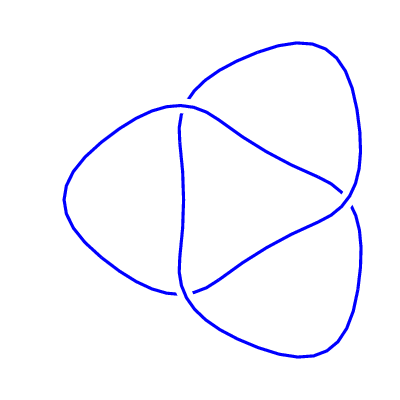
\includegraphics[width=\linewidth]{../data/3_1.png}
        \subcaption{$3_1$}
    \end{minipage}
    \begin{minipage}[b]{.14\linewidth}
        \centering
        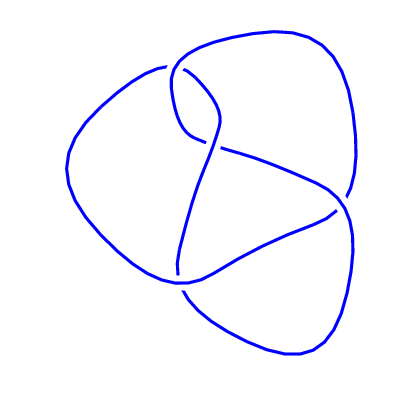
\includegraphics[width=\linewidth]{../data/4_1.png}
        \subcaption{$4_1$}
    \end{minipage}
    \begin{minipage}[b]{.14\linewidth}
        \centering
        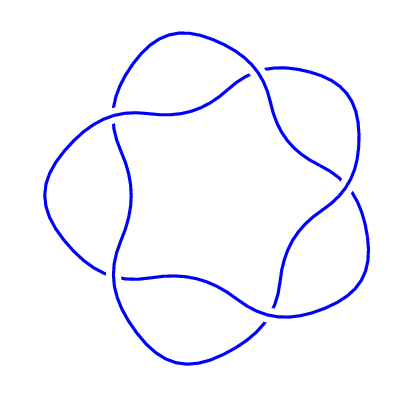
\includegraphics[width=\linewidth]{../data/5_1.png}
        \subcaption{$5_1$}
    \end{minipage}
    \begin{minipage}[b]{.14\linewidth}
        \centering
        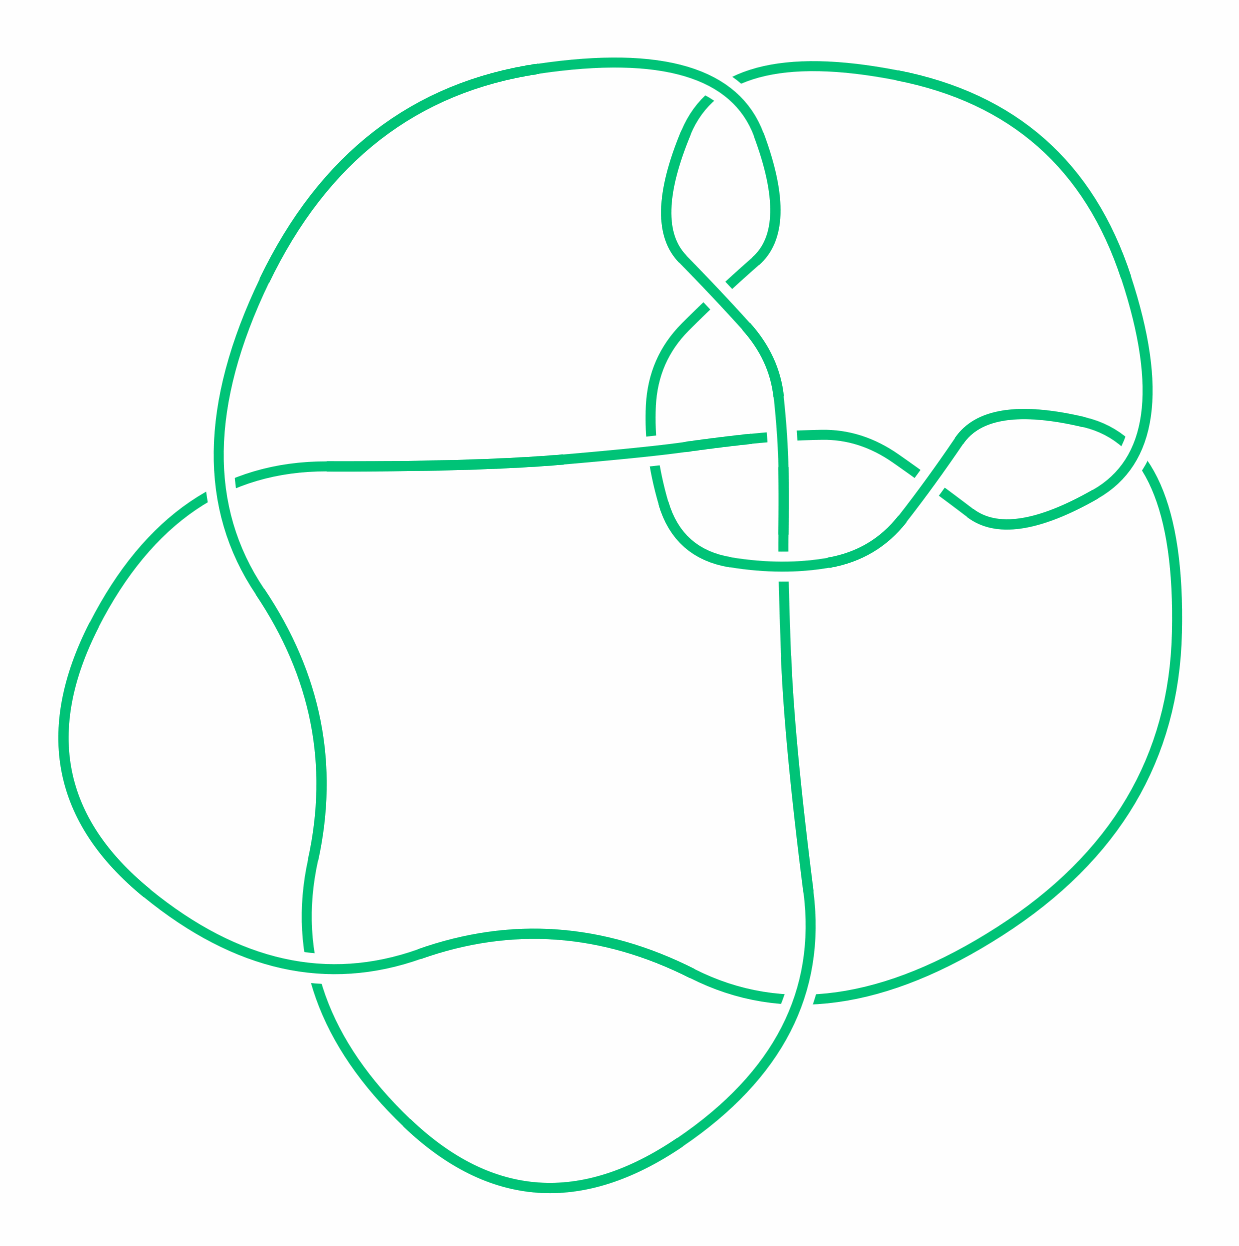
\includegraphics[width=\linewidth]{../data/perko1.png}
        \subcaption{$10_{161}$}
    \end{minipage}
    \begin{minipage}[b]{.14\linewidth}
        \centering
        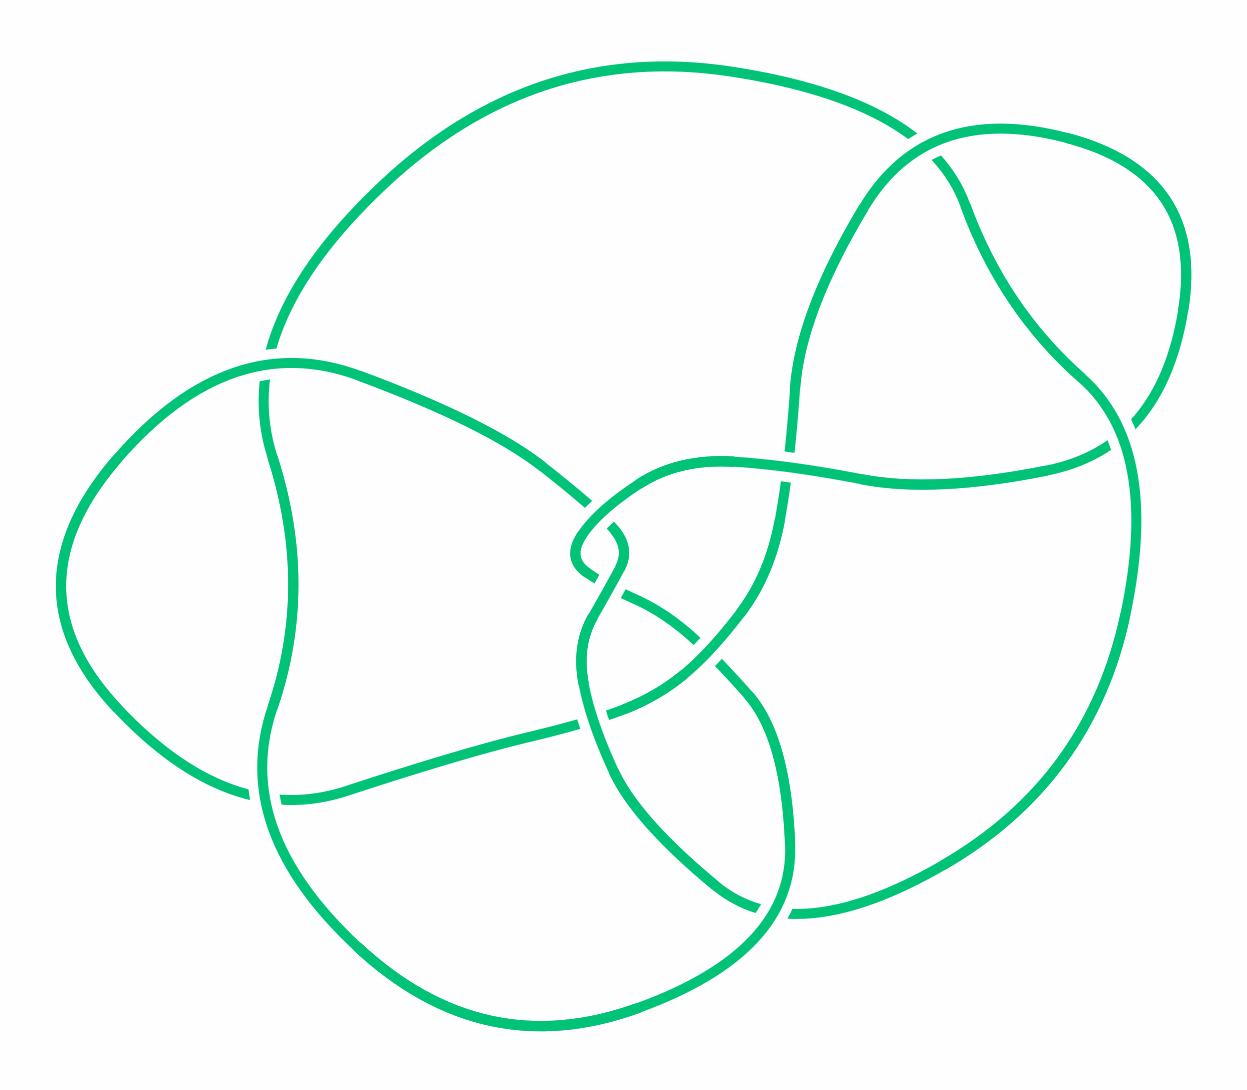
\includegraphics[width=\linewidth]{../data/perko2.png}
        \subcaption{$10_{162}$}
    \end{minipage}
\end{figure}

Początkowo celem teorii węzłów była klasyfikacja wszystkich węzłów.
Od XIX wieku, kiedy teoria węzłów wyodrębniła się jako osobny dział matematyki,
zdążyliśmy skatalogować ponad sześć miliardów tych obiektów.
Pozornie tak samo wyglądające węzły mogą się od siebie różnić.
Do wykrywania tych subtelnych różnic używa się przede wszystkim niezmienników topologicznych takich jak grupy, wielomiany bądź liczby.
Poznamy je w~dalszych rozdziałach.

Matematycy uogólnili pojęcie węzła:
można rozpatrywać je w~wyższych wymiarach albo zastąpić okrąg inną przestrzenią topologiczną.
Będziemy starać się unikać tych uogólnień.

\section{Węzły i~sploty}
Największą różnicą między węzłami matematycznymi oraz tymi z~prawdziwego jest życia jest to, że te pierwsze nie mają luźnych końców.
Można przyjąć nieidealną, naiwną definicję:

\begin{definition}[węzeł]
    Ciągłe oraz różnowartościowe odwzorowanie $S^1 \to \R^3$ nazywamy węzłem.
\end{definition}

Niestety, dopuszcza ona patologiczne z~kombinatorycznego punktu widzenia węzły dzikie, jak ten z~rysunku \ref{wild_knot}:

\begin{figure}
    \centering
    \label{wild_knot}
    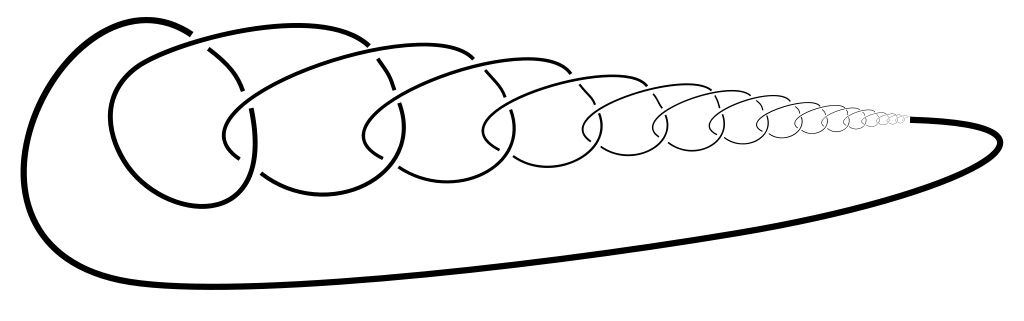
\includegraphics[width=0.5\linewidth]{wild_knot.png}
    \caption{Węzeł dziki}
\end{figure}

Zastanówmy się, jakim formalizmem opisać manipulowanie fizycznym sznurkiem, by wykluczyć węzły dzikie z~naszych rozważań.
Nie można użyć izotopii (dwa węzły są izotopijne, jeśli istnieje ciągła funkcja $F \colon S^1 \times [0, 1] \to \R^3$ taka, że $F(-, 0)$ jest pierwszym, zaś $F(-,1)$ drugim węzłem), gdyż każdy węzeł jest izotopijny z punktem:

{\color{red}\textbf{Tu brakuje obrazka.}}

W podobny sposób moglibyśmy przekształcić dowolny węzeł w~niewęzeł.
Teoria, w~której wszystkie obiekty są takie same, nie jest zbyt ciekawa.
Zwykła izotopia nie oddaje dobrze tego, czym jest równoważność węzłów wykonanych z~prawdziwego sznurka.
Trzeba od niej wymagać dodatkowo, by była gładka albo lokalnie płaska.
Z twierdzenia o rozszerzaniu izotopii wynika, że można ją wtedy podnieść do izotopii otaczającej.
Ta ostatnia uwzględnia, jak węzeł leży w~przestrzeni i okazuje się być właściwym pojęciem równości dla teorii węzłów:

\begin{definition}[izotopia otaczająca] \label{def_ambient_isotopy}
    Niech $N, M$ będą rozmaitościami, zaś $K_1, K_2 \colon N \to M$ włożeniami.
    Ciągłe odwzorowanie $F \colon M \times [0,1] \to M$ spełniające następujące warunki:
    \begin{enumerate}
        \item funkcja $F(-, 0)$ jest odwzorowaniem tożsamościowym,
        \item każda z funkcji $F(-, t)$ jest homeomorfizmem,
        \item złożenie $F(-, 1)$ z pierwszym włożeniem $K_1$ daje drugie włożenie $K_2$
    \end{enumerate}
    nazywamy izotopią otaczającą przenoszącą $K_1$ na $K_2$.
\end{definition}

W topologii rozważa się włożenia dowolnych rozmaitości, nam wystarczy jeden szczególny przypadek $N = S^1$ oraz $M = \R^3$.
Intuicyjnie, funkcja $F$ zniekształca przestrzeń $\R^3$ tak, że w~chwili początkowej $t = 0$ widzimy pierwszy, zaś w~chwili końcowej $t = 1$ drugi węzeł.
Izotopia otaczająca nie pozwala na ściąganie zaplątanych fragmentów do punktu.

{\color{red}\textbf{Homeomorfizmy $F_t$ można zastąpić przez dyfeomorfizmy zachowujące orientację. ???}}

\begin{definition}[węzeł]
    \label{def:knot}
    \index{węzeł}
    Gładkie włożenie $S^1 \to \R^3$ otaczająco izotopijne z~zamkniętą łamaną bez samoprzecięć nazywamy węzłem poskromionym.
\end{definition}

Przez prawie całą książkę interesować nas będą jedynie węzły poskromione,
dlatego jeśli nie zaznaczono inaczej, przez węzeł rozumiemy węzeł poskromiony.
Istnieje jeszcze jedna, konkurencyjna definicja węzłów równoważnych:

\begin{proposition}
    \label{equivalent_knots_2}
    Dwa węzły są równoważne, gdy jeden z~nich jest obrazem drugiego przez zachowujący orientację homeomorfizm $\R^3 \to \R^3$.
\end{proposition}

Stwierdzenie to przestaje być prawdziwe po zastąpieniu przestrzeni $\R^m$ przez $S^m$.

\begin{proof}
    Podany niżej dowód pochodzi z~książki ,,Topology from the differentiable viewpoint'' Johna Milnora.
    Musimy pokazać, że dyfeomorfizm $f \colon \R^m \to \R^m$ jest gładko izotopijny z~identycznością.
    Translacje są izotopiami, więc bez straty ogólności zakładamy, że $f(0) = 0$.
    Pochodna $f$ w~zerze jest dana wzorem $\mathrm{d}f_0(x) = \lim_{t \to 0} f(tx) /t$,
    naturalną definicję izotopii $F \colon \R^m \times [0, 1] \to \R^m$ stanowi więc
    \[
        F(x, t) = \begin{cases}
            \mathrm{d}f_0(x) & t = 0 \\
            f(tx) / t & 0 < t \le 1
        \end{cases} .
    \]

    Funkcja $F$ jest gładka, gdyż na mocy lematu Hadamarda funkcja $f$ zapisuje się jako suma $x_1 g_1(x) + \ldots + x_mg_m(x)$,gdzie funkcje $g_i$ są gładkie, co jakoś kończy dowód.
\end{proof}

Formalnie węzły to pewne odwzorowania, więc prawidłowym sposobem na zapisanie, że są izotopijne (czyli dla nas: równe), jest $K_1 \simeq K_2$.
Ponieważ nie prowadzi to do problemów, będziemy jednak stosować zapis $K_1 = K_2$.
Jednocześnie często węzeł (jako odwzorowanie) nie będzie odróżniany od obrazu tego odwzorowania.

\begin{definition}[splot, ogniwo]
    \label{def_link}
    \index{splot}
    Sumę parami rozłącznych węzłów $K_1, K_2, \ldots, K_n$ nazywamy splotem.
    Składniki sumy nazywamy ogniwami.
\end{definition}

Przez analogię do węzłów mówimy, że dwa sploty są takie same, jeśli jeden jest obrazem drugiego przez zachowujący orientację homeomorfizm $\R^3 \to \R^3$.
W~takiej sytuacji obydwa sploty mają tyle samo ogniw.

\begin{example}
    \index{splot!Hopfa}
    Splot Hopfa to najprostszy splot nietrywialny, którym w~1931 r. zajmował się Heinz Hopf, topolog niemiecki, w~ramach badań nad tzw. rozwłóknieniem (Hopf fibration).
    Whitehead w~1934 odkrył kontrprzykład do nieudanego dowodu hipotezy Poincarego.
    Był nim splot o~dwóch składowych przedstawiony na poniższym rysunku.

    \begin{figure}[H]
        \begin{minipage}[b]{.48\linewidth}
            \centering
            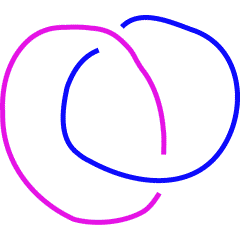
\includegraphics[width=0.5\linewidth]{../data/mixed/L2a1.png}
            \subcaption{splot Hopfa}
        \end{minipage}
        \begin{minipage}[b]{.48\linewidth}
            \centering
            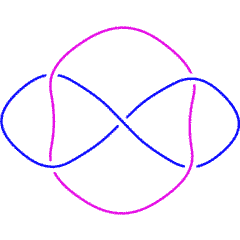
\includegraphics[width=0.5\linewidth]{../data/mixed/L5a1.png}
            \subcaption{splot Whiteheada}
        \end{minipage}
    \end{figure}
\end{example}

Jeśli dwa węzły są równoważne, to ich dopełnienia są oczywiście homeomorficzne.
Pytanie o~prawdziwość implikacji odwrotnej jako pierwszy zadał najprawdopodobniej w~1908 roku Tietze (,,Über die topologischen Invarianten mehrdimensionaler Mannigfaltigkeiten'').
W roku 1987 pokazano, że istnieją co najwyżej dwa węzły o~zadanym dopełnieniu (\cite{culler87}).
Dwa lata później poznaliśmy pozytywną odpowiedź na pytanie Tietzego: każdy węzeł jest wyznaczony jednoznacznie przez swoje dopełnienie.

\begin{theorem}[Gordon, Luecke, 1989]
    \label{thm_gordon_luecke}
    \index{twierdzenie!Gordona-Lueckego}
    Poskromione węzły o~homeomorficznych (z zachowaniem orientacji) dopełnieniach są wzajemnie izotopijne.
\end{theorem}

\begin{proof}[Niedowód]
    Wynika to z~ogólniejszego stwierdzenia:
    nietrywialna chirurgia Dehna na węźle w~3-sferze nigdy nie daje 3-sfery.
    Pełny dowód zawiera praca \cite{gordon89}.
\end{proof}

Twierdzenie to zamienia problem lokalny (czy dwa węzły w kuli $S^3$ są równoważne?) w~problem globalny (czy dwie przestrzenie topologiczne są homeomorficzne?).
Whitehead w~pracy \cite{whitehead37} z~1937 roku podał nieskończenie wiele splotów, których dopełnienia wyglądają jak dopełnienia splotu Whiteheada.
Odpowiednik twierdzenia \ref{thm_gordon_luecke} dla splotów jest więc fałszywy.

Poniższa definicja nie jest nam jeszcze potrzebna, ale wygodnie przytoczyć ją już teraz.

\begin{definition}[rozszczepialność]
    \index{splot!rozszczepialny}
    Jeżeli splot $L$ można zanurzyć w przestrzeni $\R^3$ tak, że niektóre jego ogniwa będą leżeć nad pewną rozłączną ze splotem płaszczyzną, zaś pozostałe pod nią, to powiemy, że splot $L$ jest rozszczepialny.
\end{definition}

Liczbę nierozszczepialnych splotów, pierwszych lub złożonych, zebrano w tabeli.
Źródło: baza danych OEIS, ciąg \href{https://oeis.org/A086825}{A086825}.

\renewcommand*{\arraystretch}{1.4}
\footnotesize
\begin{longtable}{lccccccccc}
    \hline
    \textbf{skrzyżowania}  &  0  &  1  &  2  &  3  &  4  &  5  &  6   &  7   &  8   \\  \hline  \endhead
    sploty                 &  1  &  0  &  1  &  1  &  3  &  4  &  15  &  24  &  82  \\
    \hline
\end{longtable}
\normalsize

\section{Diagramy. Ruchy Reidemeistera}
Chociaż w~świetle definicji \ref{def:knot} węzły są pewnymi regularnymi podzbiorami przestrzeni $\R^3$,
z kombinatorycznego punktu widzenia wygodniej jest rysować je na płaszczyźnie.

\begin{definition}[orientacja]
    \index{węzeł!zorientowany}
    Węzeł, w~którym wybrano kierunek, w~którym należy się po nim poruszać, nazywamy zorientowanym.
\end{definition}

\begin{definition} [diagram] \label{def_diagrams}
    \index{diagram}
    Cień to rzut węzła $K \subseteq \R^3$ na płaszczyznę.
    Cień razem z~informacją o~tym, jak przebiegają skrzyżowania i pozbawiony katastrof: potrójnych przecięć, stycznych czy dziobów nazywamy diagramem.
\end{definition}

{\color{red}\textbf{Narysować katastrofy}}

\begin{definition} [włókno]
    \index{włókno}
    Fragment diagramu, który biegnie między dwoma kolejnymi tunelami, czyli podskrzyżowaniami, nazywamy włóknem.
\end{definition}

\begin{definition} [nić]
    \index{nić}
    Fragment diagramu, który biegnie między dwoma kolejnymi skrzyżowaniami nazywamy nicią.
\end{definition}

Nici powstają z włókien przez rozcięcie ich przy każdym nadskrzyżowaniu.

\begin{proposition}
    Niech $K$ będzie węzłem.
    Zbiór diagramów jest otwarty i~gęsty w~zbiorze wszystkich rzutów.
\end{proposition}

\begin{proof}
    Rzut splotu na równoległe płaszczyzny jest taki sam, a te można sparametryzować prostymi przechodzącymi przez początek układu współrzędnych, które tworzą przestrzeń rzutową $\R \mathbb P^2$.
    Niech $S$ będzie zbiorem prostych, które dają złe rzuty.
    Wystarczy pokazać jego nigdziegęstość.
    Okazuje się, że $S$ jest też jednowymiarowy.
    (Dowód za \cite{crowell63}).
\end{proof}

Wynika stąd, że każdy węzeł ma wiele diagramów.
Mając dane dwa różne diagramy chcielibyśmy wiedzieć, czy reprezentują ten sam węzeł.
Na szczęście Reidemeister w latach 20. XX wieku podał proste kryterium rozstrzygające ten problem.
Najpierw zdefiniujmy trzy lokalne operacje na diagramach.

\begin{definition}
    \index{ruchy Reidemeistera}
    Trzy ruchy Reidemeistera, $R_1$, $R_2$, oraz $R_3$, to następujące deformacje diagramu:
    \[
        \underbrace{\begin{tikzpicture}[baseline=-0.65ex,scale=0.1]
        \begin{knot}[clip width=5]
            \strand[thick] (-5, 10) to [in=left, out=down] (2, -5);
            \strand[thick] (5, 0) to [in=right, out=down] (2, -5);
            \strand[thick] (5, 0) to [in=right, out=up] (2, 5);
            \strand[thick] (-5, -10) to [in=left, out=up] (2, 5);
        \end{knot}
        \end{tikzpicture}
        \, \cong \,
        \begin{tikzpicture}[baseline=-0.65ex,scale=0.1]
        \begin{knot}[clip width=5]
            \strand[thick] (0,10) to (0,-10);
        \end{knot}
        \end{tikzpicture}}_{R_1}
        %%%
        \quad \quad \quad
        \underbrace{\begin{tikzpicture}[baseline=-0.65ex,scale=0.1]
        \begin{knot}[clip width=5]
            \strand[thick] (-5, 10) to [in=up, out=down] (5, 0);
            \strand[thick] (-5, -10) to [in=down, out=up] (5, 0);
            \strand[thick] (5, 10) to [in=up, out=down] (-5, 0);
            \strand[thick] (5, -10) to [in=down, out=up] (-5, 0);
        \end{knot}
        \end{tikzpicture}
        \, \cong \,
        \begin{tikzpicture}[baseline=-0.65ex,scale=0.1]
        \begin{knot}[clip width=5]
            \strand[thick] (-5, 10) to [in=up, out=down] (-2, 0);
            \strand[thick] (-5, -10) to [in=down, out=up] (-2, 0);
            \strand[thick] (5, 10) to [in=up, out=down] (2, 0);
            \strand[thick] (5, -10) to [in=down, out=up] (2, 0);
        \end{knot}
        \end{tikzpicture}}_{R_2}
        %%%
        \quad \quad \quad
        \underbrace{\begin{tikzpicture}[baseline=-0.65ex,scale=0.1]
        \begin{knot}[clip width=5, flip crossing/.list={1,2,3}]
            \strand[thick] (-10, -10) -- (10, 10);
            \strand[thick] (-10, 10) -- (10, -10);
            \strand[thick] (-10, 0) to [in=left, out=right] (0, 10);
            \strand[thick] (10, 0) to [in=right, out=left] (0, 10);
        \end{knot}
        \end{tikzpicture}
        \, \cong \,
        \begin{tikzpicture}[baseline=-0.65ex,scale=0.1]
        \begin{knot}[clip width=5, flip crossing/.list={1,2,3}]
            \strand[thick] (-10, -10) -- (10, 10);
            \strand[thick] (-10, 10) -- (10, -10);
            \strand[thick] (-10, 0) to [in=left, out=right] (0, -10);
            \strand[thick] (10, 0) to [in=right, out=left] (0, -10);
        \end{knot}
        \end{tikzpicture}}_{R_3}
    \]
\end{definition}

Ruch $R_i$ operuje więc na $i$ łukach diagramu.
Reidemeister w~swojej pierwszej pracy przyjął inną kolejność,
jego drugi ruch jest naszym pierwszym.

\begin{theorem}[Reidemeister, 1927]
    \label{thm:reidemeister}
    Każdy splot posiada diagram.
    Dwa diagramy przedstawiają równoważne sploty,
    wtedy i~tylko wtedy gdy pierwszy można otrzymać z~drugiego
    wykonując skończenie wiele ruchów Reidemeistera
    oraz gładko deformując łuki bez zmiany biegu skrzyżowań.
\end{theorem}

Twierdzenie Reidemeistera jest prawdziwe zarówno dla splotów zorientowanych jak i~takich, które nie posiadają orientacji.

\begin{proof}
    Szkielet dowodu można znaleźć w~książce Burdego i~Zieschanga.
    Kluczowe pomysły zawiera ,,Knots, links, braids and $3$-manifolds''
    Prasołowa i~Sosińskiego.
    Innym przystępnym źródłem jest podręcznik \cite{murasugi96} Murasugiego ,,Knot theory and its applications''.
\end{proof}

{\color{red}\textbf{Brakuje prawdziwych cytowań}}

W praktyce twierdzenia \ref{thm:reidemeister} nie stosuje się bezpośrednio do diagramów splotów.
Jednym z~powodów jest wynik Cowarda i~Lackenby'a (\cite{coward11}): jeśli na dwóch diagramach tego samego węzła widać łącznie $n$ skrzyżowań, to ,,wystarcza''
\[
    R(n) = 2^{2^{\ldots^{2^n}}}
\]
ruchów Reidemeistera, by przejść między nimi; piętrowa potęga ma $10^{1000000n}$ warstw.
Gdy jeden z~diagramów jest pozbawiony skrzyżowań, czyli przedstawia niewęzeł, wystarcza $(236n)^{11}$ ruchów.
Zapewne lepsze ograniczenia istnieją, ale ich nie znamy.
Ważne jest to, że wielkość $R(n)$ jest skończona.

{\color{red}\textbf{Przedstawić rozumowanie (piramidka z węzłami), dlaczego to nie jest takie oczywiste.}}

Zamiast tego definiuje się niezmienniki, czyli funkcje ze zbioru wszystkich diagramów, które nie zmieniają swojej wartości podczas wykonywania ruchów Reidemeistera.
Kiedy pewien niezmiennik przyjmuje różne wartości na dwóch diagramach, te przedstawiają dwa istotnie różne sploty.
Gdy wartości są te same, nie dostajemy żadnej informacji.
Sploty mogą być równoważne albo nie.
Niezmienniki będą nam stale towarzyszyć w~wędrówce po krainie węzłów.

% koniec sekcji Ruchy Reidemeistera

%Niestety pomimo upływu czasus, nikt nie napisał komputerowego programu realizującego ten algorytm (stan na 1994).
%Może podejmie się tego Czytelnik?
%Inne algorytmy istnieją, jednak wszystkie działają w~wykładniczym czasie.

W 1961 roku W. Haken \cite{haken61} podał niezawodny przepis na wykrycie diagramu niewęzła,
częściowo rozwiązując jeden z~ważniejszych problemów teorii węzłów.
Przez wiele lat nikt nie podjął się implementacji tego algorytmu,
udało się to niedawno Burtonowi, Budneyowi oraz Petterssonowi w~komputerowym programie Regina\footnote{Dostępny pod adresem \url{https://regina-normal.github.io/}.} na przełomie tysiącleci.
Burton, Rubinstein i~Tillman pokazali w~pracy \cite{burton12}, jak sprawdzać,
czy powierzchnia normalna na striangulowanej 3-rozmaitości jest (nie)ściśliwa w~czasie wykładniczym.
To okazało się być wystarczającym do udzielenia negatywnej odpowiedzi na pytanie Thurstona:
,,czy przestrzeń Seiferta-Webera jest rozmaitością Hakena?'',
a zatem wykraczającego poza poziom tej pracy.
Patrz także {\url{http://geometrygames.org/SnapPea/index.html}.

{\color{red}\textbf{Dowiązać tutaj wszystkie wykrywacze niewęzła opisane w książce}}

Przykładami trudnych w~rozpoznaniu niewęzłów są: niewęzeł Goritza, Freedmana.
Więcej trudnych niewęzłów zawiera praca \cite{zanellati16} autorstwa C. Petronio oraz A. Zanellatiego.

\begin{figure}[H]
    \begin{minipage}[b]{.32\linewidth}
        \centering
        
\includegraphics[width=\linewidth]{../data/missing.jpg}
        \subcaption{normalny}
    \end{minipage}
    \begin{minipage}[b]{.32\linewidth}
        \centering
        
\includegraphics[width=\linewidth]{../data/missing.jpg}
        \subcaption{Goritza}
    \end{minipage}
    \begin{minipage}[b]{.32\linewidth}
        \centering
        
\includegraphics[width=\linewidth]{../data/missing.jpg}
        \subcaption{Freedmana}
    \end{minipage}
\end{figure}

Zanim opowiemy, jak dotąd przebiegała klasyfikacja węzłów o małej liczbie skrzyżowań, zdefiniujemy klasę splotów ze specjalnymi diagramami.

\begin{definition}[alternacja]
    \index{węzeł!alternujący}
    Diagram splotu, gdzie podczas poruszania się wzdłuż każdego ogniwa nad- oraz podskrzyżowania mijane są naprzemiennie, nazywamy alternującym.
    Splot jest alternujący, jeśli posiada alternujący diagram.
\end{definition}

Około 1961 roku Fox zapytał ,,What is an alternating knot?''.
Szukano takiej definicji węzła alternującego, która nie odnosi się bezpośrednio do diagramów, aż w~2015 roku Joshua Greene podał geometryczną charakteryzację: nierozdzielczy splot w $S^3$ jest alternujący wtedy i tylko wtedy, gdy ogranicza dodatnią oraz ujemną określoną powierzchnię rozpinającą \cite{greene17}.
% definite spanning surface

Sundberg oraz Thistlethwaite pokazali w 1998 roku, że liczba splotów alternujących rośnie wykładniczo (\cite{sundberg98}):

\begin{proposition}
    Niech $a_n$ oznacza liczbę pierwszych, alternujących supłów o~$n$ skrzyżowaniach.
    Wtedy
    \begin{equation}
        a_n \sim (3c_1/4\sqrt{\pi})n^{-5/2}\lambda^{n-3/2},
    \end{equation}
    gdzie zarówno $c_1$, pierwszy współczynnik rozwinięcia Taylora funkcji $\Phi(\eta)$ zdefiniowanej w \cite{sundberg98}, jak i $\lambda$ są jawnie znanymi stałymi:
    \begin{align}
        c_1 & = \sqrt{\frac{5^7 \cdot (21001 + 371 \sqrt{21001})^3}{2 \cdot 3^{10} \cdot (17 + 3\sqrt{21001})^5}} \\
        \lambda & = \frac {1}{40} (101 + \sqrt{21001})
    \end{align}
    Niech $A_n$ oznacza liczbę pierwszych, alternujących splotów o $n$ skrzyżowaniach.
    Wtedy $A_n \approx \lambda^n$, dokładniej: jeśli $n \ge 3$, to
    \begin{equation}
        \frac{a_{n-1}}{16n - 24} \le A \le \frac{a_n - 1}{2}.
    \end{equation}
\end{proposition}

Czasami będziemy używać słów przed ich zdefiniowaniem, tak jak uczyniliśmy tutaj: węzły pierwsze i~supły pojawiają się odpowiednio w definicjach \ref{primeknot}, \ref{def:tangle}.
Książkę trzeba więc przeczytać co~najmniej dwa razy.

\begin{proposition}
    Niech $a_n$ oznacza liczbę pierwszych, alternujących supłów o~$n$ skrzyżowaniach.
    Wtedy funkcja tworząca $f(z) = \sum_n a_n z^n$ spełnia równanie
    \begin{equation}
    f(1+z) - f(z)^2 - (1+f(z))q(f(z)) -z - \frac{2z^2}{1-z} = 0,
    \end{equation}
    gdzie $q(z)$ jest pomocniczą funkcją
    \begin{equation}
        q(z) = \frac{2z^2 - 10z - 1 + \sqrt{(1-4z)^3}} {2(z+2)^3} - \frac{2}{1+z} -z + 2.
    \end{equation}
\end{proposition}

Fakt ten stanowi raczej ciekawostkę i także pochodzi z cytowanej wcześniej pracy \cite{sundberg98}.

\subsection{Historia tablic węzłów}
Pierwszą osobą, która podjęła się szukania węzłów, był Peter Guthrie Tait, szkocki fizyk.
Razem z Thomsonem (lordem Kelvinem) wierzyli, że węzły są kluczem do zrozumienia widma spektroskopowego różnych pierwiastków: na przykład atom sodu mógł być splotem Hopfa ze względu na dwie linie emisyjne.
Eksperyment Michelsona-Morleya z 1887 roku zabił ich ,,wirową teorię atomu'', ale nie miało to znaczenia dla teorii węzłów jako działu matematyki.

Używana po dziś dzień strategia, którą przyjął Tait, jest stosunkowa prosta: narysować wszysktie możliwe diagramy o~zadanym indeksie skrzyżowaniowym, po czym połączyć ze sobą te, które przedstawiają jeden węzeł.
Na potrzeby pierwszego etapu Tait wymyślił schemat kodowania diagramów.
Wiele lat wcześniej, Gauss wraz ze swoim uczniem Listingiem badał węzły i~opracował (niezależnie!) podobną notację.
My przytoczymy opis dalszego ulepszenia tej metody, zwanego notacją Dowkera-Thistletwaite’a.

Tait wykorzystując swoją notację podał w~1876 pierwszą tablicę piętnastu węzłów o~mniej niż ośmiu skrzyżowaniach.
Nie należy traktować tego jako skromny wynik: nie miał on do dyspozycji żadnych twierdzeń topologicznych do odróżniania węzłów.
Onieśmielony przez liczbę możliwych ciągów dla kolejnych indeksów skrzyżowaniowych, powstrzymał się przed rozszerzaniem swojej tablicy.
To właśnie grupowanie diagramów przedstawiających ten sam węzeł, a~nie samo szukanie wszystkich możliwych diagramów, sprawia trudność.

Aby sobie pomóc, Tait znalazł lokalną modyfikację diagramu, która nie zmienia indeksu skrzyżowaniowego, znaną obecnie jako flype.

\[
\begin{tikzpicture}[baseline=-0.65ex, scale=0.1]
\begin{knot}[clip width=5, end tolerance=1pt, flip crossing/.list={1}]
    \strand[semithick] (-21, -5) [in=180, out=0] to (-7, 5);
    \strand[semithick] (-21, 5) [in=180, out=0] to (-7, -5);
    \draw (-7, -7) rectangle (7, 7);
    \node at (0, 0) {\Huge {$T$}};
    \draw[semithick] (7, -5) to (21, -5);
    \draw[semithick] (7, 5) to (21, 5);
\end{knot}
\end{tikzpicture}
\quad \cong_{\mathrm{flype}} \quad
\begin{tikzpicture}[baseline=-0.65ex, scale=0.1]
\begin{knot}[clip width=5, end tolerance=1pt]
    \strand[semithick] (21, -5) [in=0, out=180] to (7, 5);
    \strand[semithick] (21, 5) [in=0, out=180] to (7, -5);
    \draw (-7, -7) rectangle (7, 7);
    \node at (0, 0) {\rotatebox[origin=c]{-180}{\Huge $T$}};
    \draw[semithick] (-7, -5) to (-21, -5);
    \draw[semithick] (-7, 5) to (-21, 5);
\end{knot}
\end{tikzpicture}
\]

Inną taktykę szukania węzłów przyjał wielebny Thomas Kirkman: zaczynał od małego zbioru "nieredukowalnych" rzutów, do których systematycznie dokładał skrzyżowania.
Tait przeczytał pracę Kirkmana, po czym w~latach 1884/1885 opracował listę węzłów alternujących o~mniej niż 11 skrzyżowaniach.
Tuż przed oddaniem jej do druku odkrył inny spis węzłów stworzony przez amerykańskiego naukowca Charlesa Little'a.
Znalazł wtedy jeden duplikat u~siebie, natomiast u Little'a jeden duplikat i~jedno pominięcie.

Zachęcony przez Taita, Little zabrał się za alternujące węzły o~11 skrzyżowaniach i~za trudniejsze zadanie, stablicowanie węzłów niealternujących, czyli takich, które nie posiadają alternującego diagramu.
Jak wynika z~pierwszej pracy Taita, początkowo nie wierzono, że takie w~ogóle istnieją.
Dowód znaleziono wiele lat później, niealternujące są $8_{19}$, $8_{20}$, $8_{21}$, ale nie pierwsze węzły o mniejszej liczbie skrzyżowań.
Patrz twierdzenie \ref{prp:bankwitz}.
Little pracował przez sześć lat (1893 -- 1899) i~znalazł 43 niealternujące węzły o~10 skrzyżowaniach.
Żadnego nie pominął, ale trafił mu się jeden duplikat.

W kolejnych dziesięcioleciach nie nastąpił znaczący postęp, zarówno w~rozszerzaniu tablic jak i~sprawdzaniu tych już istniejących.
Haseman w~1918 roku znalazł achiralne węzły o~12 i~14 skrzyżowaniach.
W 1927 roku Alexander z~Briggsem przy użyciu pierwszej grupy homologii rozgałęzionego nakrycia cyklicznego (!) potrafili odróżnić od siebie dowolne dwa węzły (z~pominięciem trzech par) o~co najwyżej 9 skrzyżowaniach.
Reidemeister poradził sobie z~tymi wyjątkami w~1932 roku, korzystając z~indeksu zaczepienia i~homomorfizmów z~grupy węzła na grupy diedralne.
% branch curves in irregular covers associated to homomorphisms of the knot group onto dihedral groups

%%%%% Tait, Little wyprodukowali prawie bezbłędną tablicę węzłów o~co najwyżej 11 skrzyżowaniach przy użyciu grafów.

Dopiero Conway w~latach sześćdziesiątych minionego wieku znalazł pierwsze węzły o~mniej niż 12 skrzyżowaniach oraz wszystkie sploty o~mniej niż 11 skrzyżowaniach w~oparciu o~pomysły Kirkmana.
% An enumeration of knots and links, 1970.
Zajęło mu to jedynie kilka godzin!
Conway znalazł 1 duplikat oraz 11 pominięć w~tablicach Little'a, ale sam popełnił 4 pominięcia.
Przeoczył między innymi słynny duplikat w~niealternującej tablicy Little'a, parę Perko.
% 1974?
Przyczyną było prawdopodobnie to, że dwa diagramy miały różny spin:
Little błędnie twierdził, że spin minimalnego diagramu jest niezmiennikiem, gdyż błędnie założył, że flype oraz 2-przejścia wystarczają do zmiany jednego minimalnego diagramu w~inny.

Pominęcia w~tablicy Conwaya znalazł Caudron w~1980 roku.
Nieopublikowany manuskrypt Bonahona, Siebenmanna klasyfikuje węzły algebraiczne.
Z~nielicznymi niealgebraicznymi węzłami do 11 skrzyżowań poradził sobie Perko około 1980 roku (,,Invariants of 11-crossing knots'').
To był kres ery ręcznych obliczeń.

Na początku lat osiemdziesiątych Dowker i~Thistlethwaite stabularyzowali z~pomocą komputera węzły do 13 skrzyżowań.
Przez blisko dekadę nic się nie działo, aż grupa studentów wygrała dostęp do superkomputera Cray.
Razem z~Hoste znaleźli alternujące węzły do 14 skrzyżowań, jednocześnie sprawdzając istniejące tabele Thistlethwaite'a.
Około roku 1998 Hoste z~Weeksem (oraz niezależnie Thistlethwaite) znaleźli 1701936 pierwszych węzłów do 16 skrzyżowań.
Spośród nich, tylko 32 nie jest węzłami hiperbolicznymi, wszystkie pozostałe poddają się maszynerii geometrii hiperbolicznej.

\subsection{Hipotezy Taita}
\begin{conjecture}[I hipoteza Taita]
    \label{conj_tait_i}
    \index{hipoteza!Taita}
    Zredukowany alternujący diagram splotu ma minimalny indeks skrzyżowaniowy.
\end{conjecture}
% To bardzo ważny rezultat, którego prawdziwość przypuszczał już P. G. Tait w~XIX wieku.
% Nikt nie był w~stanie podać dowodu przed pojawieniem się wielomianu Jonesa.

Najpierw znaleziono dowód korzystający z wielomianu Jonesa (Kauffman \ref{kauffman87}, Murasugi \ref{murasugi87}, Thistlethwaite \ref{thistlethwaite87}, wszystkie prace z 1987 roku).
Trzydzieści lat później Greene zaprezentował geometryczne podejście do problemu w \ref{greene17}.

\begin{conjecture}[II hipoteza Taita]
    \label{conj_tait_ii}
    Achiralny splot alternujący ma zerowy spin.
\end{conjecture}

Pierwsze dowody pochodzą znowu od Kauffmana \ref{kauffman87} oraz Thistlethwaite'a \ref{thistlethwaite87}.

\begin{conjecture}[III hipoteza Taita]
    \label{conj_tait_iii}
    Niech $D_1, D_2$ będą zredukowanymi alternującymi diagramami zorientowanego pierwszego splotu.
    Wtedy diagram $D_2$ można otrzymać z~$D_1$ korzystając jedynie z~ruchu \emph{flype}.
\end{conjecture}

Tę hipotezę udowodnił Menasco z Thistlethwaitem, \ref{menasco91}.
Wynika z~niej, że dwa zredukowane diagramy alternujące tego samego węzła mają ten sam spin: ruch flype nie zmienia spinu (dla niektórych to jest II hipoteza).	
My pokażemy nieco później, czyli po poznaniu wielomianu Jonesa, że wszystkie trzy hipotezy są prawdziwe.

\textbf{Wstawić odniesienia do naszego dowodu}

\subsection{Metody kodowania}
\subsubsection{Notacja Alexandera-Briggsa}
Najbardziej tradycyjna, wprowadzona w~1927 roku, rozszerzona później przez Rolfsena.

\subsubsection{Notacja Dowkera-Thistlethwaite'a}
Poprawia notację Taita.
Należy ustalić minimalny diagram węzła, dowolny punkt początkowy oraz kierunek i zacząć przemierzać węzeł.
Za każdym razem, kiedy mijamy skrzyżowanie, przypisujemy mu kolejną liczbę naturalną, zaczynając od jedynki.
Jeżeli znajdujemy się nad skrzyżowaniem, parzyste etykiety zapisujemy z przeciwnym znakiem.
Kiedy skończymy, każde skrzyżowanie będzie mieć dwie etykiety.

\begin{definition}
	Ciąg parzystych liczb występujących na diagramie kolejno przy $1, 3, \ldots$ nazywamy kodem Dowkera-Thistlethwaite'a.
\end{definition}

Opisany powyżej kod nie jest idealny, ponieważ odtworzony z niego węzeł może być lustrzanym odbiciem wyjściowego.
Ogólniej, odbicie dowolnego składnika sumy spójnej nie zmienia kodu całego węzła.
Nie stanowi to jednak dużego problemu, ponieważ notacja została stworzona na potrzeby tablicowania węzłów pierwszych, a~te są niezorientowane.

Zaczynając od zredukowanego diagramu o $n$ skrzyżowaniach nie można doprowadzić do sytuacji, gdzie do pewnego skrzyżowania przypisane są dwie kolejne liczby całkowite.
Dzięki temu problem można przetłumaczyć na język teorii grafów.
Rozpatrzmy graf $G$, którego wierzchołkami są liczby $1, 2, \ldots, 2n$.
Połączmy niesąsiadujące modulo $2n$ wierzchołki o różnej parzystości krawędziami.
Graf ten powstaje przez usunięcie cyklu Hamiltona (łączącego kolejne liczby) z pełnego grafu dwudzielnego.
Zbiór par etykiet przy skrzyżowaniach węzła to skojarzenie doskonałe w grafie $G$.
Liczba skojarzeń prawie pokrywa się z rozwiązaniem zadania znanego w literaturze jako ,,problème des ménages'': na ile sposobów $n$ małżeństw można posadzić przy okrągłym stole tak, by żadne małżeństwo nie siedziało obok siebie i~każdy mężczyzna znalazł się obok dwóch kobiet?
Ustawienia, które powstają przez cykliczne permutowanie należy uznać za tożsame.
Gilbert znalazł w \cite{gilbert56} wzór na $a_n$, liczbę różnych kodów:
\begin{align}
u(m, t) & = 2m \sum_{k=0}^m {2m-k \choose k} \cdot (m-k)! \cdot \frac{(t-1)^k}{2m - k}  \\
a(n) & = \frac{1}{n} \sum_{d\mid n} \left(\frac{n}{d}\right)^d \cdot u \left(d, 1 - \frac{d}{n}\right) \cdot \varphi \left(\frac{n}{d}\right)
\end{align}

Kilka początkowych wartości to $a_3 = 1, 2, 5, 20, 87, 616, 4843, 44128, 444621, \ldots$ (ciąg A002484 w OEIS).

\subsubsection{Notacja Conwaya}
Wprowadzona przez Conwaya w~pracy \cite{conway70}.
Opiera się na pojęciu supła, dlatego więcej szczegółów przedstawiamy dopiero w definicji \ref{conway_notation}.

% A pictorial enumeration of prime knots of up to 10 crossings appears in Rolfsen (1976, Appendix C).
% Note, however, that in this table, the Perko pair 10-161 and 10-162 are actually identical, and the uppermost crossing in 10-144 should be changed (Jones 1987).

% Rolfsen's last four 10 crossing knots have been renumbered, to avoid the Perko duplication.
% A further mistake in Rolfsen's tables is that therein 1083 and 1086 were swopped: the Conway notation and Alexander polynomial for each one referred to the diagram of the other.
% We exchange not diagrams, but Alexander polynomial and Conway notation to fix the mistake (like the table in the new 2003 edition of the Rolfsen book, Dror Bar-Natan's Knot Atlas, and Chuck Livingston's Table of Knot Invariants, and unlike in Kawauchi's book!).
% http://stoimenov.net/stoimeno/homepage/ptab/

\section{Operacje na węzłach} % (fold)
W tej sekcji poznamy sposoby otrzymywania nowych obiektów z~już istniejących (rewers i~lustro splotu).
Rodzina węzłów wyposażona w~sumę spójną tworzy przemienny monoid z~jednoznacznością rozkładu.
Znacznie później (w sekcji \ref{sec:tangle}) określimy jeszcze sumę oraz iloczyn supłów.

\subsection{Lustro i~rewers} % (fold)
\begin{definition}[lustro]
    \index{lustro}
    \index{węzeł!lustrzany}
    Niech $L$ będzie zorientowanym splotem.
    Splot $mL$ powstały przez odbicie splotu $L$ względem dowolnej płaszczyzny nazywamy lustrem.
\end{definition}

\begin{definition}[rewers]
    \index{rewers}
    \index{węzeł!odwrotny}
    Niech $L$ będzie zorientowanym splotem.
    Splot $rL$ powstały przez odwrócenie orientacji wszystkich ogniw splotu $L$ nazywamy rewersem.
\end{definition}

\begin{comment}
\begin{figure}[H]
    \begin{minipage}[b]{.32\linewidth}
        \centering
        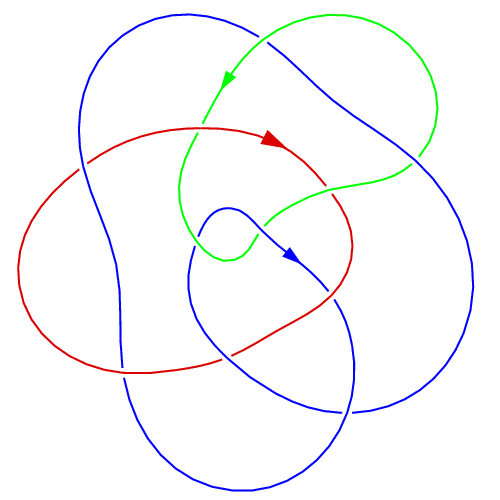
\includegraphics[width=\linewidth]{../data/link_mirror.png}
        \subcaption{lustro $mL$}
    \end{minipage}
    \begin{minipage}[b]{.32\linewidth}
        \centering
        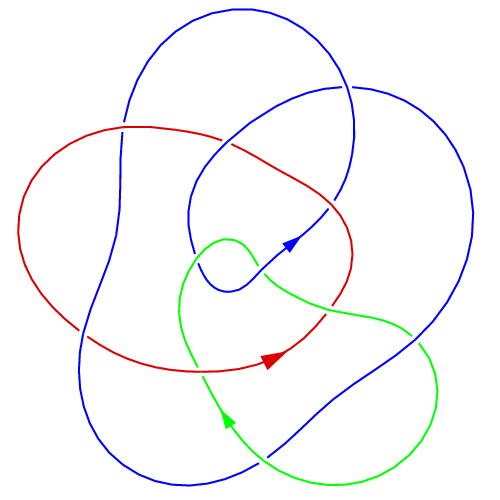
\includegraphics[width=\linewidth]{../data/link.png}
        \subcaption{przykładowy splot $L$}
    \end{minipage}
    \begin{minipage}[b]{.32\linewidth}
        \centering
        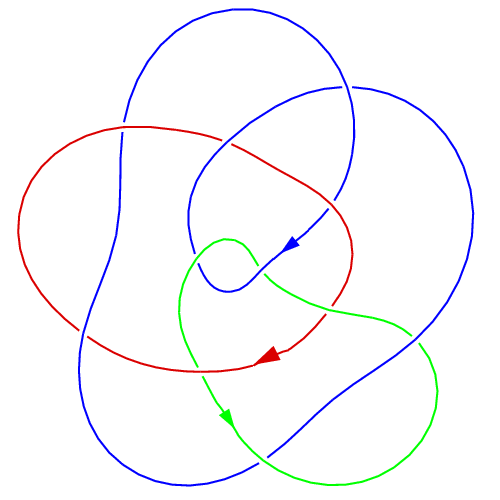
\includegraphics[width=\linewidth]{../data/link_reverse.png}
        \subcaption{rewers $rL$}
    \end{minipage}
\end{figure}
\end{comment}

Na lewym obrazku odbiliśmy diagram względem poziomej prostej, innym sposobem na otrzymanie lustra jest odwrócenie wszystkich skrzyżowań, co odpowiada odbijaniu względem płaszczyzny papieru.
Zauważmy, że wykonując powyższe operacje na węźle możemy otrzymać mniej niż czterech różne obiekty ($L$, $mL$, $rL$, $mrL$) -- na przykład trójlistnik jest własnym rewersem, ale nie lustrem.

Wyróżniamy pięć typów symetrii węzłów:

\begin{definition}[całkowicie chiralny albo skrętny]
    \index{węzeł!chiralny (skrętny)}
    Węzły $K$, $rK$, $mK$ są parami nierównoważne. % chiral 9_32
\end{definition}

\begin{definition}[odwracalny]
    \index{węzeł!odwracalny}
    Węzły $K \cong rK$ są równoważne. % reversible 3_1
\end{definition}

\begin{definition}[zwierciadlany ujemnie]
    \index{węzeł!zwierciadlany}
    Węzły $K \cong mrK$ są równoważne. % negative amphicheiral 8_17
\end{definition}

\begin{definition}[zwierciadlany dodatnio]
    Węzły $K \cong mK$ są równoważne. % positive amphicheiral 12a_427
\end{definition}

\begin{definition}[całkowicie zwierciadlany]
    Węzły $K, rK, mK$ są parami równoważne. % fully amphicheiral 4_1
\end{definition}

\begin{example}
    Węzeł $9_{32}$ jest całkowicie skrętny.
\end{example}

Całkowicie skrętne są też między innymi wszystkie węzły torusowe.

\begin{example}
    \label{exm:trefoil_is_chiral}
    Trójlistnik jest odwracalny, ale nie zwierciadlany.
\end{example}

Po raz pierwszy odkrył to M. Dehn w 1914 roku \cite{dehn14}.
Oto, jak tego dokonał.
Iloraz grafu Cayleya dla grupy podstawowej trójlistnika, $G = \pi_1(S^3 - K)$, zanurza się w~produkt $\mathbb H^2 \times \R$, co pozwala wyznaczyć grupę zewnętrznych automorfizmów grupy $G$, $\Z/2\Z$.
\index{grupa!podstawowa}
Korzystając z południków i równoleżników pokazał następnie, że nietrywialny automorfizm odwraca orientację przestrzeni otaczającej.
My przekonamy się o~tym przez wyznaczenie wielomianu Jonesa trójlistnika, patrz wniosek \ref{cor:joines_of_amphicheiral}.

\begin{example}
    Węzeł $8_{17}$ jest zwierciadlany ujemnie, ale nie odwracalny.
\end{example}

Sześćdziesiąt lat temu matematycy nie byli pewni, czy węzły nieodwracalne w~ogóle istnieją \cite[problem 10]{fox62};
obecnie wiadomo, że nieodwracalne są prawie wszystkie węzły (\cite[s.~46]{murasugi96}).
W~roku 1962 Ralph Fox wskazał kilku kandydatów do tego tytułu.
Hale Trotter odkrył rok później nieskończoną rodzinę nieodwracalnych precli, patrz \ref{prp:pretzel_not_invertible}.

\begin{example}
    Węzeł $12a427$ jest zwierciadlany dodatnio, ale nie odwracalny.
\end{example}

Żaden inny węzeł pierwszy o mniej niż 13 skrzyżowaniach nie ma tej cechy.

\begin{example}
    Ósemka $4_1$ jest całkowicie zwierciadlana.
\end{example}

To najprostszy typ symetrii, wystarczy jawnie wskazać przekształcenie między diagramem węzła, jego lustra oraz odwrotności.

Tait odnosił wrażenie, że zwierciadlane węzły mają parzysty indeks skrzyżowań,
ale Hoste (Thistlethwaite?) znalazł w~1998 kontrprzykład o~piętnastu skrzyżowaniach.
Jest on jedynym znanym nam dzisiaj.
Hipoteza Taita jest prawdziwa dla węzłów pierwszych, alternujących.

\begin{proposition}[10.4.4 w \cite{kawauchi96}]
    Niech $K$ będzie węzłem zwierciadlanym.
    Wtedy
    \begin{align}
        V(t) & = V(1/t) \\
        P(a, z) & = P(1/a, z) \\
        F(a, z) & = F(1/a, z),
    \end{align}
    gdzie $\jones, P, F$ oznacza kolejno wielomian Jonesa, HOMFLY oraz Kauffmana.
    Równość $\conway(z) = \conway(-z)$ zachodzi dla wszystkich węzłów, zwierciadlanych lub nie.

    Patrz fakt \ref{cor:joines_of_amphicheiral}.
\end{proposition}

Poniższa tabela oparta jest (kolejno) o~ciągi
\href{https://oeis.org/A051766}{51766},
\href{https://oeis.org/A051769}{51769},
\href{https://oeis.org/A051768}{51768},
\href{https://oeis.org/A051767}{51767},
\href{https://oeis.org/A052400}{52400},
z bazy danych ``The On-Line Encyclopedia of Integer Sequences'' (OEIS).

\begin{table}[h]
    \centering
    \begin{tabular}{@{}*{20}l@{}} \toprule
        skrzyżowania & 3 & 4 & 5 & 6 & 7 & 8 & 9 & 10 & 11 & 12 & 13 & 14 \\ \midrule
        całkowicie skrętne & 0 & 0 & 0 & 0 & 0 & 0 & 2 & 27 & 187 & 1103 & 6919 & 37885 \\
        odwracalne & 1 & 0 & 2 & 2 & 7 & 16 & 47 & 125 & 365 & 1015 & 3069 & 8813 \\
        $-$ zwierciadlane & 0 & 0 & 0 & 0 & 0 & 1 & 0 & 6 & 0 & 40 & 0 & 227 \\
        $+$ zwierciadlane & 0 & 0 & 0 & 0 & 0 & 0 & 0 & 0 & 0 & 1 & 0 & 6 \\
        zwierciadlane & 0 & 1 & 0 & 1 & 0 & 4 & 0 & 7 & 0 & 17 & 0 & 41 \\
        \bottomrule
        \hline
    \end{tabular}
    \caption{Liczba węzłów o~poszczególnych typach symetrii}
\end{table}

\begin{tobedone}[Kawauchi, definicja 10.3.2]
    Węzeł $K \subseteq S^3$ jest silnie odwracalny, jeśli istnieje inwolucja pary $(S^3, K)$ która zachowuje orientację sfery, ale odwraca orientację węzła.
\end{tobedone}

Węzeł silnie odwracalny jest odwracalny, ale nie vice versa (Hartley 1980, Whitten 1981).
Chyba, że ograniczymy się do węzłów hiperbolicznych (Kawauchi proposition 10.3.3, cf. 3.2.11).
Bycie silnie odwracalnym nie narzuca żadnych ograniczeń na wielomian Alexandera (odniesienie do $u = 1$?), patrz Sakai 1983.

\subsection{Węzły okresowe}
Można wyróżnić jeszcze jeden rodzaj symetrii.

\begin{definition}
    \label{def:period}
    \index{węzeł!okresowy}
    Węzeł $K$ nazywamy $n$-okresowym, jeśli istnieje obrót $f \colon \R^3 \to \R^3$ o~kąt $2\pi/n$ wokół pewnej prostej $l$, rozłącznej z~węzłem, taki że $f(K) = K$.
\end{definition}

Zamiast obrotów można rozpatrywać dowolne odwzorowania okresowe $f \colon S^3 \to S^3$, których zbiór punktów stałych jest rozłączny z węzłem $K$, homeomorficzny z $S^1$ oraz które trzymają węzeł $K$ w miejscu, ale dostaje się wtedy dokładnie taką samą klasę węzłów.
\index{hipoteza!Smitha}
Wynika to z hipotezy Smitha, otrzymanej z połączenia głębokich teorii dotyczących geometrii i topologii 3-rozmaitości.
% Kawauchi, ćwiczenie 10.1.10
% Morgan-Bass 1984

\begin{proposition}
    Zbiór wszystkich okresów jest niezmiennikiem węzłów.
\end{proposition}

Nieodwracalny węzeł $8_{17}$ nie posiada żadnych okresów.
% ćwiczenie 10.1.5 w Kawauchi
Węzeł $5_1$ 5-okresowy, co widać na standardowym diagramie, oraz 2-okresowy, tę drugą symetrię można dostrzec na diagramie realizującym indeks mostowy.
Trójlistnik ma dokładnie dwa okresy, $2$ i~$3$.
Ogólniej, jak głosi Kawauchi \cite[ćwiczenie 10.1.9]{kawauchi96}:

\begin{proposition}
    Jedynymi okresami węzła $(p, q)$-torusowego są dzielniki liczb $p$ oraz $q$.
\end{proposition}

Z~każdym węzłem okresowym związany jest inny, prostszy węzeł.
Niech $f$ będzie obrotem z definicji \ref{def:period}, zaś $p \colon \R^3 \to \R^3/f \simeq \R^3$ rzutem na przestrzeń ilorazową.
\index{węzeł!ilorazowy}
Wtedy $p(K)$ nazywamy \emph{węzłem ilorazowym}, zaś $K$ to jego $n$-krotne nakrycie.

Murasugi podał dwa warunki, które musi spełniać węzeł o~okresie $n = p^r$, gdzie $r$ jest liczbą pierwszą.
Do ich zrozumienia potrzebujemy prostej definicji.
Ustalmy półprostą, która nie jest styczna do węzła $K$, po czym zorientujmy ją oraz węzeł.
Indeksem zaczepienia $\lambda$ węzła $p(K)$ jest różnica między liczbą skrzyżowań dodatnich oraz ujemnych wzdłuż półprostej (bez znaku).

\begin{proposition}[warunek Murasugiego]
    \index{warunek!Murasugiego}
    \label{prp:murasugi_periodic}
    Niech $K$ będzie węzłem o~okresie $n = p^r$, gdzie $p$ jest liczbą pierwszą.
    Niech $J$ będzie jego węzłem ilorazowym, z~indeksem zaczepienia $\lambda$.
    Wtedy wielomian $\alexander_J$ jest dzielnikiem wielomianu $\alexander_K$ oraz istnieje pewna całkowita liczba $k$, taka że
    \begin{equation}
        \alexander_K(t) \equiv \pm t^k \alexander_J(n)^n \left(1 + t + t^2 + \ldots + t^{\lambda - 1}\right)^{n-1} \mod p.
    \end{equation}
\end{proposition}

\begin{proof}
    Mozolne operacje na macierzach, których wyznacznikiem jest wielomian Alexandera, patrz \cite{murasugi71}.
    Kawauchi przedstawia inny dowód: najpierw dowodzi tego dla węzła torusowego $T_{n, d}$, którego węzłem ilorazowym jest niewęzeł.
    W ogólnym przypadku, korzysta z relacji kłębiastej dla wielomianu Conwaya.
    Szczegóły oraz odsyłacze do dalszych prac znaleźć można w jego przeglądowej publikacji \cite[s. 122-124]{kawauchi96}.
\end{proof}

% Koniec podsekcji Lustro i~rewers

\subsection{Suma niespójna i~suma spójna} % (fold)

Suma spójna węzłów to szczególny przypadek sklejenia dwóch rozmaitości wzdłuż brzegu.

\begin{definition}[suma niespójna]
    Niech $L_1$ oraz $L_2$ będą splotami, które leżą po różnych stronach ustalonej płaszczyzny w przestrzeni $\R^3$.
    Teoriomnogościową sumę $L_1 \sqcup L_2$ nazywamy sumą niespójną splotów.
\end{definition}

\begin{definition}[suma spójna]
    \index{suma!spójna, niespójna}
    Niech $K_1, K_2$ będą zorientowanymi węzłami.
    Natnijmy każdy z nich w dwóch punktach tego samego krótkiego łuku, a następnie zszyjmy dwoma łukami, które nie przecinają już istniejących, jak na obrazku.
    Otrzymany węzeł nazywamy sumą spójną węzłów $K_1$ oraz $K_2$.
\begin{comment}
    \[
        \begin{tikzpicture}[baseline=-0.65ex,scale=0.1]
        \begin{knot}[clip width=5, flip crossing/.list={5}, ignore endpoint intersections=false,]
            \strand[thick] (-3.5, -3.5) [in=down, out=up] to (3.5, 3.5);
            \strand[thick] (3.5, 3.5) [in=right, out=up] to (-4.5, 10);
            \strand[thick] (-4.5, 10) [in=up, out=left] to (-10, 3.5);
            \strand[thick] (-10, 3.5) to (-10, -3.5);
            \strand[thick] (-10, -3.5) [in=left, out=down] to (-4.5, -10);
            \strand[thick] (-4.5, -10) [in=down, out=right] to (3.5, -3.5);
            \strand[thick] (3.5, -3.5) [in=down, out=up] to (-3.5, 3.5);
            \strand[thick] (-3.5, 3.5) [in=left, out=up] to (4.5, 10);
            \strand[thick] (4.5, 10) [in=up, out=right] to (10, 3.5);
            \strand[thick, -Latex] (10, 3.5) to (10, -3.5);
            \strand[thick] (10, -3.5) [in=right, out=down] to (4.5, -10);
            \strand[thick] (4.5, -10) [in=down, out=left] to (-3.5, -3.5);
            \node at (0, -15) {$K_1$};
        \end{knot}
        \end{tikzpicture}
        \shrap
        \begin{tikzpicture}[baseline=-0.65ex,scale=0.1]
        \begin{knot}[clip width=5, flip crossing/.list={6}, ignore endpoint intersections=false,]
            \strand[thick] (-3.5, -3.5) [in=down, out=up] to (3.5, 3.5);
            %\strand[thick] (3.5, 3.5) [in=right, out=up] to (-4.5, 10);
            %\strand[thick] (-4.5, 10) [in=up, out=left] to (-10, 3.5);
            \strand[thick] (-10, -3.5) [in=left, out=up] to (0, 6.5);
            \strand[thick, Latex-] (-10, -3.5) [in=left, out=down] to (-4.5, -10);
            \strand[thick] (-4.5, -10) [in=down, out=right] to (3.5, -3.5);
            \strand[thick] (3.5, -3.5) [in=down, out=up] to (-3.5, 3.5);
            %\strand[thick] (-3.5, 3.5) [in=left, out=up] to (4.5, 10);
            %\strand[thick] (4.5, 10) [in=up, out=right] to (10, 3.5);
            \strand[thick] (10, -3.5) [in=right, out=up] to (0, 6.5);
            \strand[thick] (10, -3.5) [in=right, out=down] to (4.5, -10);
            \strand[thick] (4.5, -10) [in=down, out=left] to (-3.5, -3.5);
            %
            \strand[thick] (-3.5, 3.5) [in=left, out=up] to (0, 10);
            \strand[thick] (3.5, 3.5) [in=right, out=up] to (0, 10);
            \node at (0, -15) {$K_2$};
        \end{knot}
        \end{tikzpicture}
        =
        \begin{tikzpicture}[baseline=-0.65ex,scale=0.1]
        \begin{knot}[clip width=5, flip crossing/.list={5, 22, 23}, ignore endpoint intersections=false,]
            \strand[thick] (-18.5, -3.5) [in=down, out=up] to (-11.5, 3.5);
            \strand[thick] (-11.5, 3.5) [in=right, out=up] to (-19.5, 10);
            \strand[thick] (-19.5, 10) [in=up, out=left] to (-25, 3.5);
            \strand[thick] (-25, 3.5) to (-25, -3.5);
            \strand[thick] (-25, -3.5) [in=left, out=down] to (-19.5, -10);
            \strand[thick] (-19.5, -10) [in=down, out=right] to (-11.5, -3.5);
            \strand[thick] (-11.5, -3.5) [in=down, out=up] to (-18.5, 3.5);
            \strand[thick] (-18.5, 3.5) [in=left, out=up] to (-10.5, 10);
            \strand[thick] (-10.5, 10) [in=left, out=right] to (-5, 2);
            \strand[thick, -Latex] (-5, 2) to (-5+6, 2);
            \strand[thick] (5, 2) to (-5+6, 2);
            \strand[thick] (3, -2) to [in=left, out=right] (10.5, -10);
            \strand[thick, -Latex] (3, -2) to (0, -2);
            \strand[thick] (-5, -2) to (0, -2);
            \strand[thick] (-5, -2) [in=right, out=left] to (-10.5, -10);
            \strand[thick] (-10.5, -10) [in=down, out=left] to (-18.5, -3.5);
            %%%
            \strand[thick] (11.5, -3.5) [in=down, out=up] to (18.5, 3.5);
            \strand[thick] (-10 +15, 2) [in=left, out=right] to (15, 6.5);
            \strand[thick] (10.5, -10) [in=down, out=right] to (18.5, -3.5);
            \strand[thick] (18.5, -3.5) [in=down, out=up] to (11.5, 3.5);
            \strand[thick] (25, -3.5) [in=right, out=up] to (15, 6.5);
            \strand[thick] (25, -3.5) [in=right, out=down] to (19.5, -10);
            \strand[thick] (19.5, -10) [in=down, out=left] to (11.5, -3.5);
            \strand[thick] (11.5, 3.5) [in=left, out=up] to (15, 10);
            \strand[thick] (18.5, 3.5) [in=right, out=up] to (15, 10);
            %%%
            \node at (0, -15) {$K_1 \shrap K_2$};
        \end{knot}
        \end{tikzpicture}
    \]
\end{comment}
\end{definition}

\begin{tobedone}
The band sum operation is a special case of a hyperbolic transformation of a link (in 12.3) and also of a fusion of a link (in 13.1).
% Kawauchi
\end{tobedone}

Ważna jest orientacja składników: suma dwóch trójlistników może być węzłem babskim lub prostym.
Uzasadnienie, że te węzły są różne, nie jest łatwym zadaniem.
Fox pokazał w~1952 roku, że ich dopełnienia nie są homeomorficzne.
Suma przeciwnie skręconych trójlistników jest plastrowa, natomiast tak samo skręconych nie jest.
\index{węzeł!plastrowy}
(To jedno z niewielu miejsc, gdzie nomenklatura pochodzi od żeglarzy: z~angielskiego \emph{granny knot, square knot}.)

Warunku, by zszywające łuki nie przecinały diagramów, nie można pominąć: Cromwell w~\cite[s.90]{cromwell04} pokazuje przykład dwóch niewęzłów, z~których otrzymano niepoprawnie dwie różne sumy, $6_1$ oraz $8_{20}$.

Uogólnieniem sumy spójnej oraz (nieopisanej w~naszej pracy) operacji \emph{plumbing} jest suma Murasugiego, dobrze wyjaśniona w~czwartym rozdziale książki \cite{kawauchi96}.

\begin{tobedone}
The Murasugi sum of Seifert surfaces was introduced originally in [Murasugi 1958, 1958',1958"] in order to estimate the degree of the Alexander polynomial of alter- nating links. After that, J. Stallings showed in [Stallings 1978] that a Seifert surface obtained by a Murasugi sum of fiber surfaces is a fiber surface.
\end{tobedone}

% TODO: \textbf{W topologii rozważa się podobną operację dla dwóch $n$-wymiarowych rozmaitości: z~każdej z nich usuwa się kulę, po czym skleja wzdłuż brzegu kuli. Kiedy zajmujemy się węzłami, nie interesuje nas jednak struktura rozmaitości (gdyż każdy węzeł jest równoważny z okręgiem), ale zanurzenie w~otaczającą przestrzeń.}

\begin{proposition}
    Suma spójna węzłów jest dobrze określonym działaniem.
\end{proposition}

Suma spójna nie jest dobrze określona dla splotów:
nie istnieje kanoniczny wybór, które ogniwa łączyć ze sobą.

\begin{proof}
    Niech dane będą węzły $K_1$ oraz $K_2$
    oraz dwa różne łuki $\gamma_1$, $\gamma_2$,
    których można użyć do konstrukcji sumy spójnej.
    Skurczmy $K_1$, przeciągnijmy najpierw przez łuk $\gamma_1$, a~następnie wzdłuż węzła $K_2$.
    Teraz wystarczy odwrócić ten proces z~$\gamma_2$ w~miejscu $\gamma_1$.
\end{proof}

\begin{proposition}
    Suma spójna jest działaniem łącznym oraz przemiennym.
    Niewęzeł stanowi jej element neutralny.
\end{proposition}

Prosty dowód tego faktu pozostawiamy Czytelnikowi.
W języku algebry mówimy, że węzły z~sumą spójną tworzą półgrupę (tak jak liczby naturalne z działaniem dodawania).
Dużo później pokażemy, że działaniu $\shrap$ brakuje elementów przeciwnych, więc ta struktura algebraiczna nie jest grupą.

\begin{proposition}
    Niech $K_1, K_2$ będą takimi węzłami, że $K_1 \shrap K_2 = \Unknot$. Wtedy $K_1 = K_2 = \Unknot$.
\end{proposition}

\begin{proof}[Niedowód]
    Technika ta zwana jest szwindlem Mazura.
    \index{szwindel Mazura}
    Załóżmy, że $K \shrap L = \Unknot$ i~dopuśćmy wyjątkowo węzły dzikie.
    Skonstruujmy sumę $K \shrap L \shrap K \shrap \ldots$,
    przy czym kolejne składniki powinny zmniejszać się,
    aby ich suma nadal była węzłem.
    Wtedy
    \begin{align*}
        K & \simeq K \shrap [(L \shrap K) \shrap (L \shrap K) \ldots] \\
         & \simeq (K \shrap L) \shrap (K \shrap L) \shrap \ldots
         \simeq \Unknot \shrap \Unknot \shrap \ldots
         \simeq \Unknot.
    \end{align*}
    Analogicznie pokazujemy, że $L \simeq \Unknot$.
\end{proof}

\begin{tobedone}
    % Kawauchi
    Theorem 3.2.1 (Non-cancellation theorem) A connected sum L1~L2 of any two links L1 and L2 is not a trivial link unless both links L1 and L2 are trivial links.
The proof (whose details are left to the reader) is essentially obtained from the following two facts:
(1) If L1 and L2 are non-split links, then L1~L2 is a non-split link.
(2) If L1~L2 is a trivial knot, then L1 and L2 are trivial knots.
(1) is directly proved by a cut-and-paste argument of combinatorial topology. (2) is usually obtained from Schubert's result on the additivity of the knot genus (cf. 4.1.5) under the connected sum, i.e., g(Ll~L2) = geLd +g(L2) (which is also proved by a cut-and-paste argument).
\end{tobedone}

Prawdziwy dowód oparty jest na topologii algebraicznej, stanowi bezpośredni wniosek z~faktów \ref{prp:genus_detects_unknot} oraz \ref{prp:genus_of_sum}.

Półgrupę węzłów z~operacją sumy spójnej można ulepszyć do grupy na dwa sposoby:
albo poprzez zmianę działania, w~jakie jest wyposażona,
albo osłabiając definicję węzłów równoważnych.
Drugi pomysł jest dużo lepszy niż pierwszy.
Na początku lat pięćdziesiątych J. Milnor wprowadził do matematyki pojęcie zgodności
(z angielskiego \emph{concordance}), które zastąpiło zwykłą równoważność.
\index{węzeł!zgodny}
Element neutralny nowej grupy to węzły plastrowe, ich opis leży w~sekcji \ref{sec:slice}.
Zagadnienia te zakorzenione są w~czterowymiarowej topologii.

% Koniec podsekcji Suma niespójna i~suma spójna

% Koniec sekcji Operacje na węzłach

\section{Węzły pierwsze}
\label{sec:prime_knots}
Istnieje węzłowy odpowiednik liczb pierwszych.
Jest on ściśle związany z~podaną wyżej operacją sumy spójnej.
Do jego dostatecznie dobrego zrozumienia wymagana jest znajomość powierzchni Seiferta (opisanych w~sekcji \ref{sec:genus}).

\begin{definition}
    \label{primeknot}
    \index{węzeł!pierwszy}
    Nietrywialny węzeł nazywamy \textbf{pierwszym},
    kiedy nie można przedstawić go jako sumy spójnej $K_1 \shrap K_2$
    dwóch nietrywialnych węzłów $K_1, K_2$ (nie jest złożony).
\end{definition}

Okazuje się, że jeśli alternujący splot nie jest pierwszy,
to każdy jego alternujący diagram jest złożony.
Jako pierwszy fakt ten został wykazany przez Menasco w~\cite{menasco84}.
Dowód opiera się na multiplikatywności wielomianu BLM/Ho (opisuje go definicja \ref{def:blm_ho}).

Czy węzłów pierwszych jest nieskończenie wiele?
Tak (patrz fakt \ref{infty_primes}), potrafimy nawet oszacować liczbę $K_n$ węzłów pierwszych oraz $L_n$ splotów pierwszych.
W roku 1987 C. Ernst, D. Sumners w~oparciu o~wyniki Thistlethwaite'a, Kauffmana, oraz Murasugiego dotyczące węzłów alternujących pokazali w~\cite{ernst87}, że $K_n \ge \frac 1 3 (2^{n- 2} - 1)$, przy czym węzły lustrzane traktowane są jako różne.
Dokładniej:

\begin{proposition}
    Niech $f(n)$ oznacza liczbę węzłów dwumostowych o indeksie skrzyżowaniowym $n$.
    Wtedy
    \begin{equation}
        f(n) = \begin{cases}
        \frac 13 (2^{n-2} - 1) & \text{dla } n = 2k \ge 4 \\
        \frac 13 (2^{n-2} + 2^{(n-1)/2}) & \text{dla } n = 4k + 1 \ge 5 \\
        \frac 13 (2^{n-2} + 2^{(n-1)/2} + 2) & \text{dla } n = 4k + 3 \ge 7
        \end{cases}
    \end{equation}
\end{proposition}


Welsh rozpatruje w \cite{welsh92} węzły bez orientacji i znajduje poniższe ograniczenia.
Nie wiadomo, czy zwykłe granice istnieją.
\begin{equation}
    2.68 \le \liminf_{n \to \infty}  \sqrt[n]{K_n} \le \limsup_{n \to \infty} \sqrt[n]{L_n} \le \frac {27}{2}.
\end{equation}

% "On the number of knots and links" (MR1218230)

Czy niewęzeł nie daje się zapisać jako suma dwóch innych węzłów?
Byłoby to skrajnie niepożądane, gdyż każdy węzeł jest naturalnie spójną sumą siebie oraz niewęzła.
Na szczęście przy pomocy powierzchni Seiferta można pokazać, że tak się nie dzieje (jest to wniosek \ref{no_inverses}).
Prawdziwe jest dużo mocniejsze stwierdzenie,
którego nie udowodnimy ze względu na niedostatecznie rozwinięty aparat matematyczny.
Należy o~nim myśleć jak o~analogonie zasadniczego twierdzenia arytmetyki.

\begin{theorem}[Schubert, 1949]
    Każdy różny od niewęzła węzeł rozkłada się jednoznacznie na węzły pierwsze
    (jeśli tylko pominąć kolejność składników).
\end{theorem}

Pomimo to uda się nam pokazać samo istnienie rozkładu, jest to fakt \ref{genus_sum}.
% koniec sekcji Węzły pierwsze

\section{Niezmienniki liczbowe}
Jak wspomnieliśmy na początku rozdziału, sprawdzenie,
czy dwa diagramy przedstawiają sploty równoważne,
jest uciążliwym i~czasochłonnym zadaniem.
Aby je uprościć, podamy opis kilku prostych niezmienników o~całkowitych wartościach.
Zachodzą implikacje:
sploty równoważne $\Rightarrow$ ta sama wartość niezmiennika
oraz różne wartości niezmiennika $\Rightarrow$ różne sploty.

Tutaj przedstawiamy jedynie te niezmieniki, które nie wymagają mocnej znajomości reszty książki.
Później poznamy jeszcze sygnaturę (w~podsekcji \ref{sub:signature}}) oraz liczbę warkoczową (w~podsekcji \ref{sub:braid_number}).

\subsection{Indeks skrzyżowaniowy} % (fold)
\label{sub:crossing_number}
\index{indeks!skrzyżowaniowy}
Z angielskiego \emph{crossing number}.

\begin{definition}
    Niech $L$ będzie splotem.
    Minimalną liczbę skrzyżowań widocznych na diagramie, który przedstawia splot $L$, nazywamy indeksem skrzyżowaniowym i~oznaczamy $\operatorname{cr}(L)$.
\end{definition}

Pytanie, czy indeks skrzyżowaniowy jest addytywny, to jeden z najstarszych problemów teorii węzłów.

\begin{conjecture}
    \label{cnj:crossing_additive}
    Niech $K$ oraz $L$ będą węzłami.
    Wtedy $\operatorname{cr}(K) + \operatorname{cr}(L) = \operatorname{cr}(K \shrap L)$.
\end{conjecture}

Oto częściowe odpowiedzi.
Jeśli $K_1, K_2$ są alternującymi węzłami o~odpowiednio $c_1, c_2$ skrzyżowaniach, to istnieje alternujący diagram ich sumy $K_1 \shrap K_2$ o~$c_1 + c_2$ skrzyżowaniach.
Kauffman, Murasugi oraz Thistlethwaite pokazali niezależnie, że diagram ten jest minimalny (patrz na przykład \cite{murasugi87}, wniosek 6).
Thistlethwaite rozszerzył wynik do tak zwanych węzłów adekwatnych w \cite{thistlethwaite88}.
Wreszcie Gruber w \cite{gruber03} udowodnił hipotezę \ref{cnj:crossing_additive} dla węzłów torusowych.

Lackenby w~pracy \cite{lackenby09} pokazał, że dla pewnej stałej $N \le 152$ zachodzi
\begin{equation}
    \frac 1 N \sum_{i=1}^n \operatorname{cr} K_i \le \operatorname{cr} \left(\bigshrap_{i=1}^n K_i\right) \le \sum_{i=1}^n \operatorname{cr} K_i.
\end{equation}
(Tylko pierwsza nierówność jest ciekawa).
Jego argumentu wykorzystującego powierzchnie normalne nie można poprawić tak, by otrzymać stałą $N = 1$.

\begin{proposition} \label{prp:bankwitz}
    Wyznacznik splotu alternującego $L$ jest nie mniejszy od jego indeksu skrzyżowaniowego: $\det L \ge \operatorname{cr} L$.
\end{proposition}

W ten sposób pokazano, że niealternujące węzły istnieją: $\det 8_{19} = 3 < 8 = \operatorname{cr} 8_{19}$.
Bankwitz podał w 1930 niepoprawny dowód dla specjalnego przypadku, kiedy $L$ jest węzłem.
Pierwszy pełny dowód, oparty o teorię grafów, przedstawił blisko trzy dekady później Crowell w \cite{crowell59}.
Znalazł też mocniejszą nierówność $\det L + 3 \ge \operatorname{cr} L$ dla pierwszych, alternujących splotów, które nie są $(2, n)$-torusowe.
To prawie wystarczyło do rozstrzygnięcia, które z węzłów o mniej niż 10 skrzyżowaniach są alternujące.
Otwartym problemem pozostały $9_{45}$, $9_{47}$, $9_{48}$ oraz $9_{49}$.

% Koniec podsekcji Indeks skrzyżowaniowy

\subsection{Liczba gordyjska} % (fold)
\label{sub:unknotting_number}
\index{liczba!gordyjska}
Z angielskiego \emph{unknotting number}.

\begin{definition}
    Liczba gordyjska $\operatorname{u}(K)$ węzła $K$ to minimalna liczba skrzyżowań,
    które trzeba odwrócić na pewnym jego diagramie, by dostać niewęzeł.
    Liczba $u$ nie musi być osiągana przez diagram o~minimalnej liczbie skrzyżowań.
\end{definition}

Dotychczas wyznaczono liczbę gordyjską dla prawie wszystkich węzłów pierwszych o~co najwyżej dziesięciu skrzyżowaniach,
Cha i~Livingston podają następującą listę wyjątków:
$10_{11}$, $10_{47}$, $10_{51}$, $10_{54}$, $10_{61}$, $10_{76}$, $10_{77}$, $10_{79}$, $10_{100}$ (stan na rok 2008).
S. Bleiler odkrył w~\cite{bleiler84} fascynujący przykład wymiernego węzła $2$-gordyjskiego,
czego świadkiem nie może być diagram o~minimalnej liczbie skrzyżowań
(ponieważ, co jeszcze bardziej fascynujące, węzeł ten posiada tylko jeden diagram o~dziesięciu skrzyżowaniach z~trzema do odwrócenia).
Koduje go liczba $29/6$, w~tabeli węzłów figuruje jako $10_8$.
Stojmenow w~\cite{stoimenow01} pokazuje, że jeden węzeł może mieć kilka diagramów minimalnych,
z których tylko niektóre są świadkiem $1$-gordyjskości (są to między innymi $14_{36750}$ oraz $14_{36760}$.)

Coward, Lackenby dowiedli w~\cite{coward11}, że jeśli $K$ jest 1-gordyjski i~o genusie 1, to z~dokładnością do pewnej relacji równoważności, tylko jedna zmiana skrzyżowania rozwiązuje go; chyba że $K$ jest ósemką -- wtedy takie zmiany są dwie.
Kanenobu, Murakami oraz Kohn dwadzieścia lat wcześniej wiedzieli, że wymierne sploty 1-gordyjskie posiadają rozwiązujące skrzyżowanie na minimalnym diagramie (\cite{kanenobu86}, \cite{kohn91}).

Jeśli odwrócenie pewnych skrzyżowań daje niewęzeł, to odwrócenie pozostałych także.
To daje proste, choć niezbyt pomocne oszacowanie liczby gordyjskiej: $2 \operatorname{u} (K) \le \operatorname{cr} (K)$.
Borodzik oraz Friedl podali niedawno całkiem mocne ograniczenia na liczbę gordyjską w~pracach \cite{borodzik14} i~\cite{borodzik15} opierając się o~parowanie Blanchfielda
(poprawiając ograniczenia z~sygnatury Levine'a-Tristrama, indeksu Nakanishiego oraz przeszkodą Lickorisha).
Dwadzieścia pięć węzłów o~co najwyżej dwunastu skrzyżowaniach ma liczbę gordyjską równą co najmniej trzy, co trudno pokazać innymi metodami.

Dla każdego nietrywialnego splotu istnieje diagram wymagający odwrócenia dowolnie wielu skrzyżowań (dowód zawiera praca \cite{taniyama09} Taniyamy).
Pokazany jest tam jeszcze jeden godny uwagi fakt.
Jeśli liczba gordyjska diagramu $D$ wynosi $\frac 12 (c(D) - 1)$,
co jest maksymalną możliwą wartością zgodnie z~naszym prostym ograniczeniem,
to węzeł jest $(2,p)$-torusowy albo wygląda jak diagram niewęzła po pierwszym ruchu Reidemeistera.

% Liczba gordyjska nietrywialnego węzła skręconego (definicja \ref{twist_knots}) to jeden, wystarczy bowiem rozwiązać jego splecione końce.
Patrz także stwierdzenie \ref{torus_unknotting}.

Suma dwóch węzłów $1$-gordyjskch jest $2$-gordyjska, pokazał to Scharleman.
Od początku teorii węzłów podejrzewano dużo więcej:

\begin{conjecture}
    Niech $K, J$ będą węzłami.
    Wtedy $u(K \shrap J) = u(K) + u(J)$, czyli liczba gordyjska jest addytywna.
\end{conjecture}

Z tej nieudowodnionej do dzisiaj (stan na 2018) hipotezy można wyciągnąć wniosek,
że jeśli do rozwiązania węzła wystarcza odwrócenie skrzyżowania, to jest pierwszy.
Podejrzewał to H. Wendt w~1937 roku,
kiedy policzył liczbę gordyjską węzła babskiego używając homologii rozgałęzionego nakrycia cyklicznego.

\begin{proposition}
    Węzły $1$-gordyjskie są pierwsze.
\end{proposition}

\begin{proof}[Niedowód]
    W pracy \cite{scharleman85} z~1985 roku M. Scharleman podał dość zawiłe uzasadnienie, w~które zamieszane były grafy planarne.
\end{proof}

W pracy \cite{shimizu14} Ayaka Shimizu rozpatruje różne operacje, które rozwiązują węzły lub sploty.
Na przykład zamiana pod- i nadskrzyżowań wokół obszaru na diagramie rozwiązuje węzły, ale nie sploty.
Kontrprzykładem jest splot Hopfa.

Liczbę gordyjską można uogólnić w naturalny sposób do metryki.
Mianowicie mając dane dwa węzły $K_0, K_1$, rozpatrzmy wszystkie homotopie $f : [0,1] \times S^1 \to \R^3$ takie, że wszystkie funkcje $f_t$ są zanurzeniami z co najwyżej jednym punktem podwójnym.
Zażądajmy dodatkowo, by styczne do krótkich łuków, które przecinają się w tym punkcie, były od siebie różne.
Odległością gordyjską między węzłami $K_0, K_1$ jest minimalna liczba podwójnych punktów, jakie posiada homotopia $f$.

Przestrzeń węzłów z~tą metryką bywa sprzeczna z~intuicją: twierdzenie C~z~pracy \cite{gambaudo05} głosi, że zawiera ona prawie idealną kopię przestrzeni euklidesowej dowolnego wymiaru.
Dokładniej:

\begin{proposition}
    Dla każdej liczby całkowitej $n \ge 1$ istnieje funkcja $\xi: \Z^n \to \mathcal{K}$, dodatnie stałe $A, B, C$ oraz norma $\|\cdot\|$ na przestrzeni $\R^n$ takie, że spełniona jest podwójna nierówność
    \[
        A\|x-y\|  - B \le d(\xi(x), \xi(y)) \le C\|x-y\|.
    \]
\end{proposition}

Dowód korzysta z grup warkoczowych, które poznamy w sekcji \ref{sec:braid}.

\begin{conjecture}[Bernhard 1994, Jablan 1998] \label{bernhard_jablan}
    Każdy węzeł $K$ posiada diagram $D$ realizujący liczbę gordyjską oraz skrzyżowanie, którego odwrócenie daje nowy węzeł $K'$ z diagramem $D'$ o mniejszej liczbie gordyjskiej: $u(D') < u(D)$.
\end{conjecture}

Gdyby hipoteza była prawdziwa, mielibyśmy dość prosty algorytm do wyznaczania liczby gordyjskiej $u(K)$: wystarczy skonstruować skończenie wiele diagramów minimalnych dla węzła $K$, odwracać kolejne skrzyżowania i szukać rekursywnie liczb gordyjskich nowych węzłów.
Hipoteza jest prawdziwa dla węzłów do jedenastu skrzyżowań (patrz baza danych KnotInfo C. Livingstona) i splotów o dwóch składowych do dziewięciu skrzyżowań, pokazał to Kohn w pracy \cite{kohn93} z 1993 (!) roku.
Brittenham, Hermiller twierdzą, że hipoteza jest fałszywa.

% Koniec podsekcji Liczba gordyjska

\subsection{Liczba mostowa} % (fold)
\label{sub:bridge_index}
\index{liczba!mostowa}
Z angielskiego \emph{bridge number}.
Wprowadzona w~1954 przez Schuberta.
\begin{definition}
    Liczba mostowa $\operatorname{br}(K)$ to minimalna liczba mostów:
    długich łuków, które biegną przez nadskrzyżowania.
\end{definition}

Można pokazać, że $n$-mostowe węzły rozkładają się na sumę dwóch trywialnych $n$-supłów.

\begin{proposition}
    \label{bridge_additive}
    Niech $K_1, K_2$ będą węzłami.
    Wtedy $\operatorname{br} (K_1) + \operatorname{br}(K_2) = \operatorname{br}(K_1 \# K_2) + 1$.
\end{proposition}

\begin{proof}[Nieedowód]
    Schubert pokazał to blisko pół wieku temu w~\cite{schubert54}.
    Nowszy dowód pochodzi od Schultensa, w~artykule \cite{schultens03} skorzystał z~foliacji na brzegu węzła towarzyszącego sateltarnemu.
    Dokładniejszy opis powyższych prac wykraczałby poza zakres tego opracowania, zostanie więc pominięty.
\end{proof}

Tylko jeden węzeł jest jednomostowy, to niewęzeł.
Kolejne w~hierarchii skomplikowania, czyli dwumostowe,
to domknięcia wymiernych supłów, patrz fakt \ref{prp:two_bridge_tangle}.
Węzły trójmostowe pozostają nie do końca zbadane.

\begin{conjecture}
    Jeśli $K$ jest węzłem, to $c(K) \ge 3 br(K) - 3$, przy czym równość zachodzi dokładnie dla niewęzła, trójlistnika i~sumy spójnej trójlistników (rozdział 4.3 z~podręcznika \cite{murasugi96}).
\end{conjecture}

Nie istnieje związek między liczbą mostową oraz gordyjską.
Po pierwsze, węzły torusowe $T_{2,n}$ są dwumostowe, a~ich liczba gordyjska jest duża.
Po drugie, podwojenie węzła (poza specjalnymi przypadkami, jak pokazał Schubert) zwiększa liczbę mostową dwukrotnie; liczba gordyjska takiego podwojenia wynosi $1$.
Podobnie nie ma zależności między liczbą mostową oraz genusem.

% Koniec podsekcji Liczba mostowa

\subsection{Indeks zaczepienia} % (fold)
\label{sub:linking_number}
\begin{definition} \label{sign_def}
    Na diagramie zorientowanego splotu, każdemu skrzyżowaniu przypisujemy \textbf{znak} równy $\pm 1$.
    Skrzyżowania dodatnie nazywamy praworęcznymi, ujemne zaś: leworęcznymi.
    \[
        \sign \Bigl(\,\,\begin{tikzpicture}[baseline=-0.65ex,scale=0.07]
        \begin{knot}[clip width=5]
        \strand[semithick,-Latex] (-5,-5) -- (5,5);
        \strand[semithick,Latex-] (-5,5) -- (5,-5);
        \end{knot}\end{tikzpicture}\,\,\Bigr) = +1 \quad
        \sign \Bigl(\,\,\begin{tikzpicture}[baseline=-0.65ex,scale=0.07]
        \begin{knot}[clip width=5, flip crossing/.list={1}]
        \strand[semithick,-Latex] (-5,-5) -- (5,5);
        \strand[semithick,Latex-] (-5,5) -- (5,-5);
        \end{knot}\end{tikzpicture}\,\,\Bigr) = -1
    \]
\end{definition}

\begin{definition} \label{sign_def}
    \index{indeks!zaczepienia}
    Niech $L = K_1 \sqcup K_2$ będzie splotem o dwóch ogniwach.
    Wielkość
    \[
        \operatorname{lk}(K_1, K_2) = \frac 12 \sum_i \sign c_i,
    \]
    gdzie sumowanie rozciąga się na wszystkie skrzyżowania, gdzie spotykają się łuki z różnych ogniw, nazywamy \textbf{indeksem zaczepienia} węzłów $K_1, K_2$.
    Ogólniej, jeśli $L = K_1 \sqcup \ldots \sqcup K_n$ jest splotem o $n$ ogniwach, to jego indeks zaczepienia wyznacza wzór $\operatorname{lk}(L) = \sum_{i < j} \operatorname{lk}(K_i, K_j)$.
\end{definition}

Zauważmy, że indeks zaczepienia splotu Hopfa wynosi $1$, natomiast splotu Whiteheada $0$.
Są zatem istotnie różne.
W obydwu przypadkach indeks zaczepienia jest liczbą całkowitą, nie stanowi to przypadku.
Na mocy twierdzenia Jordana $\operatorname{lk}$ jest funkcją o całkowitych wartościach.

\begin{proposition}
    Indeks zaczepienia jest dobrze określonym niezmiennikiem zorientowanych splotów.
\end{proposition}

\begin{proof}
    Sprawdźmy wpływ ruchów Reidemeistera na wartość
    $\operatorname{lk}(L)$:

    \[
        \fbox{
        \begin{tikzpicture}[baseline=-0.65ex,scale=0.07]
        \begin{knot}[clip width=5]
        \strand[semithick] (-10,10) .. controls (-10,2) and (-10,2) .. (-6,-2);
        \strand[semithick] (-10,-10) .. controls (-10,-2) and (-10,-1) .. (-9,0);
        \strand[semithick] (-7,1) -- (-6,2);
        \strand[semithick] (-6,2) .. controls (2,9) and (2,-9) .. (-6,-2);
        \end{knot}
        \end{tikzpicture}
        $\stackrel{R_1}{\cong} \,\,$
        \begin{tikzpicture}[baseline=-0.65ex,scale=0.07]
        \begin{knot}[clip width=5]
        \strand[semithick] (0,10) -- (0,-10);
        \end{knot}
        \end{tikzpicture}}
        %%%
        \quad \fbox{
        \begin{tikzpicture}[baseline=-0.65ex,scale=0.07]
        \begin{knot}[clip width=5]
        \strand[semithick] (4,-10) .. controls (4,-4) and (-4,-4) .. (-4,0);
        \strand[semithick] (4,10) .. controls (4, 4) and (-4, 4) .. (-4,0);
        \strand[semithick] (-4,-10) .. controls (-4,-4) and (4,-4) .. (4,0);
        \strand[semithick] (-4,10) .. controls (-4, 4) and (4,4) .. (4,0);
        \node[blue] at (-4,4)[left] {$a$};
        \node[blue] at (-4,-4)[left] {$-a$};
        \end{knot}
        \end{tikzpicture}
        $\stackrel{R_2}{\cong} \,\,$
        \begin{tikzpicture}[baseline=-0.65ex,scale=0.07]
        \begin{knot}[clip width=5]
        \strand[semithick] (4,-10) .. controls (4,-4) and (1,-4) .. (1,0);
        \strand[semithick] (4,10) .. controls (4, 4) and (1, 4) .. (1,0);
        \strand[semithick] (-4,-10) .. controls (-4,-4) and (-1,-4) .. (-1,0);
        \strand[semithick] (-4,10) .. controls (-4, 4) and (-1,4) .. (-1,0);
        \end{knot}
        \end{tikzpicture}}
        %%%
        \quad \fbox{
        \begin{tikzpicture}[baseline=-0.65ex,scale=0.07]
        \begin{knot}[clip width=5, flip crossing/.list={1,2,3}]
        \strand[semithick] (-10,-10) -- (10,10);
        \strand[semithick] (-10,10) -- (10,-10);
        \strand[semithick] (-10,-2) .. controls (-4, -2) and (-4,8) .. (0,8);
        \strand[semithick] (10,-2) .. controls (4, -2) and (4,8) .. (0,8);
        \node[blue] at (-6,4)[left] {$a$};
        \node[blue] at (6,4)[right] {$b$};
        \node[blue] at (0,-2)[below] {$c$};
        \end{knot}
        \end{tikzpicture}
        $\stackrel{R_3}{\cong} \,\,$
        \begin{tikzpicture}[baseline=-0.65ex,scale=0.07]
        \begin{knot}[clip width=5, flip crossing/.list={1,2,3}]
        \strand[semithick] (-10,-10) -- (10,10);
        \strand[semithick] (-10,10) -- (10,-10);
        \strand[semithick] (-10,2) .. controls (-4, 2) and (-4,-8) .. (0,-8);
        \strand[semithick] (10,2) .. controls (4, 2) and (4,-8) .. (0,-8);
        \node[blue] at (-6,-4)[left] {$a$};
        \node[blue] at (6,-4)[right] {$b$};
        \node[blue] at (0,2)[above] {$c$};
        \end{knot}
        \end{tikzpicture}}
    \]
    Na mocy twierdzenia Reidemeistera dowód został zakończony.
\end{proof}

\subsection{Spin} % (fold)
\label{sub:writhe}
Przypomnijmy, że znak skrzyżowania na diagramie to liczba $1$ lub $-1$ (definicja \ref{sign_def}).

\begin{definition}[spin]
    \index{spin}
    Wielkość
    \begin{equation}
        w(D) = \sum_c \operatorname{sign} c,
    \end{equation}
    gdzie sumowanie przebiega po wszystkich skrzyżowaniach diagramu $D$ zorientowanego splotu lub węzła, nazywamy spinem.
    Z angielskiego \emph{writhe}.
\end{definition}

Co ważne, spin nie jest niezmiennikiem splotów ani węzłów.
Para Perko przedstawia ten sam węzeł z~minimalną liczbą skrzyżowań i~spinem równym siedem lub dziewięć.
Dzięki temu przez wiele lat nie została dostrzeżona.
Spin jest za to niezmiennikiem węzłów alternujących, mówi o~tym druga hipoteza Taita.

\begin{lemma}
    Spin nie zależy od orientacji.
    Tylko I ruch Reidemeistera zmienia spin: $w(\MalyreidemeisterIa) = w(\MalyreidemeisterIb )-1$, pozostałe ruchy nie mają na niego wpływu.
\end{lemma}

%\begin{proof}
    %Proste ćwiczenie.
%\end{proof}

% Koniec sekcji Spin


Kawauchi definiuje jeszcze \emph{twisting number}: sumę spinów po wszystkich składowych.

% Koniec podsekcji Indeks zaczepienia

\subsection{Liczba patykowa} % (fold)
\label{sub:stick_index}
\index{liczba!patykowa}
Z angielskiego \emph{stick number}.

\begin{definition}
	Minimalną liczbę odcinków w~łamanej, która przedstawia węzeł $K$, nazywamy jego liczbą patykową i~oznaczamy $\operatorname{s}(K)$.
\end{definition}

Wielkość tę wprowadził do matematyki Randell w 1988 i~znalazł dokładną jej wartość dla niewęzła (3), trójlistnika (6) oraz ósemki (7).
Negami trzy lata później w~\cite{negami91} pokazał przy użyciu teorii grafów, że dla nietrywialnych węzłów prawdziwe są nierówności
\begin{equation}
    \frac{5+\sqrt{9 + 8 \operatorname{cr} K}}{2} \le \operatorname{s} K \le 2 \operatorname{cr} K.
\end{equation}

Trójlistnik to jedyny węzeł realizujący górne ograniczenie.
Z~pracy Elrifaia wynika, że dolne ograniczenie nie jest osiągane przez żaden węzeł o co najwyżej 26 skrzyżowaniach (\cite{elrifai06}).

Jin oraz Kim w 1993 ograniczyli liczby patykowe dla węzłów torusowych korzystając z~liczby supermostowej.
Wkrótce wynik został poprawiony przez samego Jina, w pracy \cite{jin97} znalazł dokładne wartości dla niektórych węzłów.
I~tak, jeśli $2 \le p < q \le 2p$, to $\operatorname{s} T_{p,q} = 2q$ oraz $\operatorname{s} T_{p, p-1} = 2$.
Ten sam wynik, choć dla węższego zakresu parametrów, odkryto w~\cite{greilsheimer97}.
Autorzy niezależnie od siebie znaleźli proste oszacowanie z góry dla liczby patykowej sumy spójnej:
\begin{equation}
	\operatorname{s}(K_1 \shrap K_2) \le \operatorname{s}(K_1) + \operatorname{s}(K_2) - 3.
\end{equation}

Koniec dekady przyniósł jeszcze jedną pracę McCabe'a z nierównością $\operatorname{s}(K) \le 3 + \operatorname{cr} (K)$ dla węzłów dwumostowych (\cite{mccabe98}) oraz odkrycie Calvo: jeśli ograniczymy się do łamanych o co najwyżej siedmiu odcinkach, ósemka przestaje być odwracalna.

Na początku XX wieku nierówności Negamiego poprawiono, z dołu dokonał tego Calvo w~\cite{calvo01}, z góry natomiast Huh, Oh w \cite{huh11}.
Górne ograniczenie można poprawić o $3/2$, jeżeli $K$ jest niealternującym węzłem pierwszym.
\begin{equation}
    \frac{7+\sqrt{1 + 8 \operatorname{cr} K}}{2} \le \operatorname{s} K \le \frac{3}{2} (1 + \operatorname{cr} K).
\end{equation}

% Koniec podsekcji Liczba patykowa

\subsection{Długość sznurowa} % (fold)
\label{sub:ropelength}
Długość sznurowa, z~angielskiego \emph{ropelength}, pochodzi z~fizycznej teorii węzłów, która bierze pod uwagę obiekty wykonane z~nieelastycznych materiałów

Długość sznurowa $L$ to stosunek długości węzła do jego grubości $\tau$ (mówimy, że węzeł $K$ jest grubości $\tau$, jeśli ma otoczenie rurowe bez samoprzecięć z~przekrojem poprzecznym o~promieniu $\tau$).
Przez wiele lat zastanawiano się, czy można zawiązać węzeł ze sznura o~długości jednej stopy i~promieniu jednego cala.
Nie jest to możliwe: rozumowanie oparte o~czterosieczne pokazuje, że długość sznurowa nietrywialnego węzła wynosi co najmniej $15.66$ (dla trójlistnika jest to co najmniej $16.372$).

Węzeł realizujący długość sznurową jest klasy $C^1$.

Prawdziwe są oszacowania asymptotyczne:
\[
    L = \Omega (\operatorname{cr}^{3/4}),  \quad
    L = O(\operatorname{cr} \log^5 \operatorname{cr})
\]

% Koniec podsekcji Ropelength

% Koniec sekcji Niezmienniki liczbowe


\chapter{Niezmienniki kolorowe}
Zamknęliśmy już pierwszy rozdział,
Wciąż nie pokazaliśmy jednak pełnego dowodu, że dwa konkretne węzły (na przykład niewęzeł i~trójlistnik) są od siebie różne.
Dlatego teraz podamy proste narzędzie odróżniające węzły: \emph{trójkolorowalność}, która przypisuje włóknom diagramu różne kolory.
Następnie rozszerzymy paletę do dowolnie wielu kolorów i~zastąpimy ją grupą skończoną.

Nawet ten wzmocniony wariant nie jest idealnym narzędziem klasyfikującym.
Istnieją węzły, których nie odróżnia.
Problem ten dotyka wielu późniejszych niezmienników, dość ważna hipoteza Jonesa \ref{jones_conjecture} pyta, czy wielomian Jonesa jest zupełny (tak nazywamy niezmienniki, które różnym węzłom przypisują różne wartości).
Pierwszy niezmiennik zupełny poznamy w~rozdziale czwartym.
Nie stanowi to wielkiego powodu do radości ze względu na wysoką złożoność obliczeniową.

\section{Kolorowanie splotów} % (fold)
\label{sec:colour_links}
Oto mniej mętny opis trójkolorowalności, czyli jak nietrudno się domyślić, kolorowalności trzema kolorami.
Diagram $D$ splotu $K$ jest trójkolorowalny, jeśli każdemu włóknu można przypisać jeden z trzech kolorów tak, by co najmniej dwa zostały użyte.
Wymagamy przy tym, by przy żadnym skrzyżowaniu nie spotykały się dokładnie dwa kolory.

Dla własnej wygody jako kolorów używać będziemy kolejnych liczb naturalnych $0, 1, 2, \ldots$.
Pozwala to zapisać warunek kolorowalności równaniem algebraicznym.

\begin{definition}[kolorowanie] \label{def:colour_equation}
	Niech $L$ będzie splotem, zaś $n$ liczbą naturalną.
	Mówimy, że splot $L$ jest kolorowalny modulo $n$, jeśli posiada diagram, którego włóknom można przypisać liczby całkowite $0, \ldots, n - 1$ tak, by równanie $a + b \equiv 2c$ modulo $n$ było spełnione przy każdym skrzyżowaniu oraz istniały dwa włókna różnych kolorów.
	Takie przyporządkowanie nazywamy (nietrywialnym) kolorowaniem.
	\[
		\begin{tikzpicture}[baseline=-0.65ex, scale=0.12]
			\useasboundingbox (-5, -5) rectangle (5,5);
			\begin{knot}[clip width=5, end tolerance=1pt, flip crossing/.list={1}]
				\strand[semithick] (-5,5) to (5,-5);
				\strand[semithick] (-5,-5) to (5,5);
				\node[darkblue] at (5, 5)[below right] {$c$};
				\node[darkblue] at (5, -5)[above right] {$b$};
				\node[darkblue] at (-5, 5)[below left] {$a$};
			\end{knot}
		\end{tikzpicture}
	\]
\end{definition}

Metoda ta została odkryta razem z uogólnieniem do $n$ kolorów przez Ralpha Foxa w 1956, kiedy próbował uczynić teorię węzłów bardziej przystępną\footnote{
	Niech $L$ będzie splotem, zaś $\pi$ grupą podstawową jego dopełnienia.
	Reprezentację $\rho$ dla $\pi$ na $D_{2n}$, grupę diedralną, nazywamy $n$-kolorowaniem Foxa.
	Grupa splotu generowana jest przez ścieżki z punktu bazowego w $S^3$ do brzegu rurowego otoczenia splotu, wokół południka i znowu do bazowego punktu.
	Obrazami tych generatorów są izometrie $n$-kąta foremnego, które zapisujemy jako $ts^i$ ($t$ to odbicie, zaś $s$ jest najmniejszym obrotem).
	Każdy generator odpowiada pewnemu łukowi, przypiszmy mu liczbę $i \in \Z/n\Z$.
	Dostaliśmy zwykłe kolorowanie, przystępne dla studentów.
}
dla studentów.
Opierając się tylko na definicji kolorowania oraz ruchach Reidemeistera jesteśmy w stanie wykazać pierwsze własności niezmiennika.

\begin{proposition}
	Żaden węzeł nie koloruje się modulo dwa.
\end{proposition}

\begin{proof}
	Załóżmy nie wprost, że istnieje nietrywialne kolorowanie.
	Analiza czterech możliwych skrzyżowań pokazuje,
	że włókna wychodzące z tunelu muszą mieć ten sam kolor.
	Przechodząc wzdłuż węzła widzimy jeden kolor, wbrew założeniu nie wprost.
\end{proof}

Sploty o wielu składowych są dwukolorowalne.
Wystarczy pomalować jedną składową zerem, a pozostałe jedynkami.
Sploty rozszczepialne są $n$-kolorowalne dla każdego $n \ge 2$, można skorzystać z tego samego schematu kolorowania.

\begin{proposition} \label{color_invariant}
	,,Bycie $n$-kolorowalnym'' jest niezmiennikiem węzłów.
\end{proposition}

\begin{proof}
	Wystarczy sprawdzić, jak ruchy Reidemeistera zmieniają kolory.
	Pierwszy i drugi:
	\[
		\fbox{
		\begin{tikzpicture}[baseline=-0.65ex,scale=0.07]
		\begin{knot}[clip width=5]
			\strand[semithick] (-10,10) .. controls (-10,2) and (-10,2) .. (-6,-2);
			\strand[semithick] (-10,-10) .. controls (-10,-2) and (-10,-1) .. (-9,0);

			\strand[semithick] (-7,1) -- (-6,2);
			\strand[semithick] (-6,2) .. controls (2,9) and (2,-9) .. (-6,-2);
			\node[darkblue] at (-10, 10)[below left] {$a$};
			\node[darkblue] at (-10, -10)[above left] {$b \equiv a$};
		\end{knot}
		\end{tikzpicture}
		$\stackrel{R_1}{\cong} \,\,$
		\begin{tikzpicture}[baseline=-0.65ex,scale=0.07]
		\begin{knot}[clip width=5]
			\strand[semithick] (0,10) -- (0,-10);
			\node[darkblue] at (0, 0)[left] {$a$};
		\end{knot}
		\end{tikzpicture}}
		%%%
		\quad \fbox{
		\begin{tikzpicture}[baseline=-0.65ex,scale=0.07]
		\begin{knot}[clip width=5]
			\strand[semithick] (4,-10) .. controls (4,-4) and (-4,-4) .. (-4,0);
			\node[darkblue] at (-4, -10)[above left] {$d \equiv b$};
			\strand[semithick] (4,10) .. controls (4, 4) and (-4, 4) .. (-4,0);
			\node[darkblue] at (4, 10)[below right] {$a$};
			\strand[semithick] (-4,-10) .. controls (-4,-4) and (4,-4) .. (4,0);
			\node[darkblue] at (4, 0) [right] {$c \equiv 2a-b$};
			\strand[semithick] (-4, 10) .. controls (-4, 4) and (4,4) .. (4,0);
			\node[darkblue] at (-4, 10) [below left] {$b$};
		\end{knot}
		\end{tikzpicture}
		$\stackrel{R_2}{\cong} \,\,$
		\begin{tikzpicture}[baseline=-0.65ex,scale=0.07]
		\begin{knot}[clip width=5]
			\strand[semithick] (4,-10) .. controls (4,-4) and (1,-4) .. (1,0);
			\strand[semithick] (4,10) .. controls (4, 4) and (1, 4) .. (1,0);
			\strand[semithick] (-4,-10) .. controls (-4,-4) and (-1,-4) .. (-1,0);
			\strand[semithick] (-4,10) .. controls (-4, 4) and (-1,4) .. (-1,0);
		\end{knot}
		\end{tikzpicture}}
	\]
	Trzeci ruch także nie wymaga skomplikowanych rachunków.
	Najkrótszy łuk na diagramach ma kolor $2a-c$ po lewej oraz $2b-c$ po prawej stronie.
	\[
	 \fbox{
		\begin{tikzpicture}[baseline=-0.65ex,scale=0.07]
		\begin{knot}[clip width=5, flip crossing/.list={1,2,3}]
			\node[darkblue] at (-10, 10) [above] {$b$};
			\node[darkblue] at (10, 10) [above] {$c$};
			\node[darkblue] at (-10, -10) [below] {$2a-2b+c$};
			\node[darkblue] at (10, -10) [below] {$2a-b$};
			\node[darkblue] at (-10, -2) [left] {$a$};
			\strand[semithick] (-10,-10) -- (10,10);
			\strand[semithick] (-10,10) -- (10,-10);
			\strand[semithick] (-10,-2) .. controls (-4, -2) and (-4,8) .. (0,8);
			\strand[semithick] (10,-2) .. controls (4, -2) and (4,8) .. (0,8);
		\end{knot}
		\end{tikzpicture}
		$\stackrel{R_3}{\cong} \,\,$
		\begin{tikzpicture}[baseline=-0.65ex,scale=0.07]
		\begin{knot}[clip width=5, flip crossing/.list={1,2,3}]
			\node[darkblue] at (-10, 10) [above] {$b$};
			\node[darkblue] at (10, 10) [above] {$c$};
			\node[darkblue] at (-10, -10) [below] {$2a-2b+c$};
			\node[darkblue] at (10, -10) [below] {$2a-b$};
			\node[darkblue] at (10, 2) [right] {$a$};
			\strand[semithick] (-10,-10) -- (10,10);
			\strand[semithick] (-10,10) -- (10,-10);
			\strand[semithick] (-10,2) .. controls (-4, 2) and (-4,-8) .. (0,-8);
			\strand[semithick] (10,2) .. controls (4, 2) and (4,-8) .. (0,-8);
		\end{knot}
		\end{tikzpicture}}
	\]
\end{proof}

Trójlistnik koloruje się dokładnie modulo krotności trójki, ósemka zaś -- piątki.
Pierścienie Boromeuszy nie kolorują się modulo trzy, nie są zatem rozszczepialne.
Sama kolorowalność nie mówi wiele, splot jest kolorowalny lub nie.
Dowód faktu \ref{color_invariant} pokazuje coś więcej: liczba kolorowań, być może trywialnych, także jest niezmiennikiem (mocniejszym).
Węzły, których żadne kolorowanie nie odróżnia od niewęzła, nazywa się czasem niewidzialnymi.

Niech $\tau_3(K)$ oznacza liczbę trójkolorowań węzła $K$.

\begin{proposition}
	Jeśli $K, L$ są węzłami, to $3\tau_3(K \shrap L) = \tau_3(K)\tau_3(L)$.
\end{proposition}

\begin{corollary}
	Istnieje nieskończenie wiele węzłów.
\end{corollary}

\begin{proof}
	Suma spójna $n$ trójlistników ma $3^n$ (być może trywialnych) $3$-kolorowań.
\end{proof}

\begin{proposition}
	Niech $n$ będzie liczbą pierwszą.
	Węzeł $p, q, r$-preclowy jest $n$-kolorowalny wtedy i tylko wtedy, gdy $n$ dzieli $|pq+qr+pr|$.
	Jeśli przynajmniej jedna z liczba $p, q, r$ nie jest wielokrotnością $n$, kolorowanie jest jedyne.
	W przeciwnym przypadku istnieją cztery kolorowania (z dokładnością do permutacji!).
\end{proposition}

\begin{proof}
	Dowód zawiera praca \emph{Counting $m$-coloring classes of knots and links} autorstwa trzech amerykanek (K. Brownell, K. O'Neil oraz L. Taalman).
	Podano tam także ogólny wzór na liczbę $n$-kolorowań dowolnego węzła.
\end{proof}

Jako kolorów użyjemy teraz elementów $g_1, \ldots, g_n$ pewnej skończonej grupy $G$.

\begin{definition}[etykietowanie]
	Mówimy, że zorientowany węzeł $K$ jest etykietowalny grupą $G$ generowaną przez elementy $g_1, \ldots, g_n$, jeśli posiada diagram, którego włóknom przypisano elementy $g_1, \ldots, g_n$ tak, by równanie $gk=hg$ było spełnione przy każdym skrzyżowaniu ($g$: włókno biegnące górą, $k$: bo jego lewej stronie, $h$: po prawej).
	\[
		\begin{tikzpicture}[baseline=-0.65ex, scale=0.12]
			\useasboundingbox (-5, -5) rectangle (5,5);
			\begin{knot}[clip width=5, end tolerance=1pt, flip crossing/.list={1}]
				\strand[semithick] (-5,5) to (5,-5);
				\strand[semithick, -Latex] (-5,-5) to (5,5);
				\node[darkblue] at (5, 5)[below right] {$g$};
				\node[darkblue] at (5, -5)[above right] {$h$};
				\node[darkblue] at (-5, 5)[below left] {$k$};
			\end{knot}
		\end{tikzpicture}
	\]
\end{definition}

Równanie $gkg^{-1}=h$ mówi, że etykiety włókien wchodzących oraz wychodzących są sprzężone.
Wynika stąd, że wszystkie etykiety pochodzą z jednej klasy sprzężoności.
Muszą jednocześnie generować całą grupę, dlatego $G$ musi być grupą nieprzemienną lub trywialną.
Etykietowalność jest niezmiennikiem węzłów i nie zależy od orientacji węzła:
jeżeli elementy $g_1, \ldots, g_n$ generują grupę, to ich odwrotności także.

Rozpatrzmy węzły $6_1$ oraz $9_{46}$ i spróbujmy etykietować je transpozycjami z grupy $S_4$.
Wybranie dwóch etykiet przy jednym skrzyżowaniu $6_1$ wymusza etykiety dla wszystkich włókien.
Dwie transpozycje nie mogą generować grupy $S_4$, natomiast włókna węzła $9_{46}$ dają się etykietować samymi transpozycjami.
Węzły te są więc różne.
Nie odróżniają ich ani kolorowania, ani wielomian Alexandera.

Livingston pisze w swojej książce,\footnote{Rozdział 5.2: Węzły i grupy} że Thistlethwaite tworząc tablice węzłów pierwszych znalazł 12965 węzłów o 13 skrzyżowaniach o 5639 różnych wielomianach Alexandera.
Używając etykietowań podgrupami grupy $S_5$ zmniejszył liczbę nierozwiązanych przypadków do mniej niż tysiąca.
Perko pokazał zaś, że każdy $S_3$-kolorowalny węzeł jest $S_4$-kolorowalny.

Niech $p \ge 3$ będzie liczbą pierwszą, natomiast $D_p = \langle r, s \mid r^p = s^2 = e, rsr = s \rangle$ grupą diedralną rzędu $2p$.
Elementy tej grupy to $1, r, r^2, \ldots, r^{p-1}, s, sr, \ldots, sr^{p-1}$.
,,Obrót'' $r^k$ jest sprzężony tylko ze swoją odwrotnością, ale ,,symetrie osiowe'' $sr^k$ tworzą jedną klasę sprzężoności.
Łatwo widać, że dowolne dwie z nich generują całą grupę $D_p$.

\begin{proposition}
	Węzeł $K$ jest $p$-kolorowalny wtedy i tylko wtedy, gdy jest $D_p$-etykietowalny.
\end{proposition}

\begin{proof}
	Załóżmy, że $K$ ma $n$ włókien.
	Wiemy już, że każde $D_p$-etykietowanie wykorzystuje tylko elementy $sr^{a_1}, \ldots, sr^{a_n}$ dla $1 \le a_i \le p$.
	Jest ono prawidłowe dokładnie wtedy, gdy analogiczne kolorowanie liczbami $a_1, \ldots, a_n$ jest prawidłowe.
\end{proof}

Etykietowania są więc uogólnieniem kolorowań.
Istnieje prosta klasyfikacja grup, których można użyć do etykietowania.

\begin{proposition}
	Niech $K$ będzie węzłem, $\pi_1$ grupą podstawową jego dopełnienia, zaś $G$ dowolną grupą.
	Następujące warunki są równoważne: $K$ jest $G$-etykietowalny; istnieje surjekcja $\pi_1 \to G$.
\end{proposition}



% Koniec sekcji Kolorowanie splotów

\section{Macierz i~wyznacznik} % (fold)
\label{sec:colour_matrix}
Zajmiemy się teraz wyznacznikiem, pierwszym nieoczywistym niezmiennikiem splotów, który przypisuje każdemu pewną liczbę całkowitą.
Jest on blisko związany z~kolorowaniem.
Zauważmy, że pierwszy ruch Reidemeistera usuwa zamknięte krzywe, czyli pojedyncze łuki bez skrzyżowań.
Diagram bez takich krzywych ma tyle samo skrzyżowań, co łuków.

\begin{definition}[macierz kolorująca]
    \index{macierz!kolorująca}
    Ustalmy diagram bez zamkniętych krzywych dla splotu $L$ z~łukami $x_0, \ldots, x_m$ oraz skrzyżowaniami $0, \ldots, m$.
    Definiujemy macierz $A_+$, której wyraz $a_{lj}$ jest współczynnikiem przy $x_j$ w~$l$-tym równaniu kolorującym:
    \[\begin{tikzpicture}[baseline=-0.65ex, scale=0.12]
    \useasboundingbox (-5, -10) rectangle (5,5);
    \begin{knot}[clip width=5, end tolerance=1pt, flip crossing/.list={1}]
        \strand[semithick] (-5,5) to (5,-5);
        \strand[semithick] (-5,-5) to (5,5);
        \node[darkblue] at (5, 5)[below right] {$x_i$};
        \node[darkblue] at (5, -5)[above right] {$x_j$};
        \node[darkblue] at (-5, 5)[below left] {$x_k$};
        \node[black] at (0, -7)[below] {$x_j+x_k - 2x_i \equiv 0 \mod n$};
    \end{knot}
    \end{tikzpicture}\]
    Macierz kolorująca $A$ powstaje z~macierzy $A_+$ przez skreślenie dowolnego wiersza i~kolumny.
\end{definition}

Taka macierz jest kwadratowa, ponieważ z~każdego skrzyżowania wychodzą (tunelem) dwa włókna mające dwa końce.
Wykreślenie wiersza i~kolumny jest konieczne.
Gdybyśmy tego zaniechali, otrzymana macierz nie byłaby odwracalna, bowiem wiersze sumują się do zera (patrz fakt \ref{prp:colouring_sum_zero}).
Dla alternujących diagramów możemy żądać, by górą $i$-tego skrzyżowania biegło $i$-te włókno, wtedy na diagonali macierzy $A$ znajdą się same minus dwójki.

\begin{definition}[wyznacznik]
    \index{wyznacznik}
    \label{def:determinant}
    Wyznacznikiem splotu nazywamy wyznacznik macierzy kolorującej $A$ bez znaku: $\det K := |\det A_K|$.
    Za wyznacznik niewęzła przyjmujemy liczbę $1$.
\end{definition}

\begin{definition}[defekt]
    Wymiar jądra macierzy kolorującej modulo $p$, defekt, nazywamy defektem węzła.
\end{definition}

Defekty modulo różne liczby pierwsze są niezależne od siebie.
Na przykład suma spójna $k$ trójlistników i~$j$ węzłów $T_{2,5}$ posiada defekt $k$ modulo $3$ oraz $j$ modulo $5$.
Podobne przykłady istnieją dla innych zbiorów liczb pierwszych.

Pokażemy później (po poznaniu grupy kolorującej, czyli we wniosku \ref{det_invariant}) lub jeszcze później (po wprowadzeniu wielomianu Alexandera, w~dowodzie faktu \ref{alexander_invariance}), że wyznacznik splotu jest dobrze określony: nie zależy on od wyboru etykietowania, minora macierzy oraz diagramu i~że jest niezmiennikiem.
Teraz ograniczymy się do jego kilku własności.

Defekt także jest niezmiennikiem, choć rzadziej używanym.
Węzeł o~defekcie $n$ modulo $p$ posiada $p(p^n-1)$ kolorowań $p$ kolorami.
Węzły $8_{18}$ oraz $9_{24}$ mają ten sam wyznacznik, $45$.
Ich defekty modulo $3$ to $1$ i~$2$, zatem są różne.

% Każde $p$-kolorowanie węzła $n$-mostowego jest wyznaczone przez kolory $n$ mostów
% % To brzmi podejrzanie: więc przestrzeń kolorowań ma wymiar co najwyżej $n$ i~defekt modulo $p$ nie przekracza $\operatorname{br} - 1$.
% Wnioskujemy stąd, że $(3,3,3)$-precel nie jest dwumostowy.

% \begin{proof}
%     \emph{Krok pierwszy}.
%     Pokażemy, że żaden ruch Reidemeistera nie zmienia wyznacznika.
%     \begin{enumerate}
%         \item \emph{Ruch $R_1$}. Diagram przed lub po ruchu zawiera co najmniej jedno włókno, które łączy tunel z~mostem pewnego skrzyżowania.
%         \item \emph{Ruch $R_2$}.
%         \item \emph{Ruch $R_3$}.
%     \end{enumerate}

%     \emph{Krok drugi}.
%     Niech $A_{i,j}$ oznacza minor powstały przez skreślenie $i$-tego wiersza oraz $j$-tej kolumny.
%     Pokażemy, że wartość wyznacznika nie zależy od wyboru $i$ oraz $j$.

%     Niech $X$ będzie macierzą $k \times k$ złożoną z~samych jedynek.
%     Suma elementów w~każdej kolumnie oraz każdym wierszu macierzy $A + X$ wynosi $k$, ponieważ znaki równań zostały dobrze wybrane.
%     Wykonujemy kolejno operacje:
%     \begin{enumerate}
%         \item Dodajemy do $i$-tego wiersza sumę pozostałych.
%         \item Dodajemy do $j$-tej kolumny sumę pozostałych.
%         Teraz $i$-ty wiersz oraz $j$-ta kolumna zawierają wyrazy $k$ z~wyjątkiem $a_{ij}$, który wynosi $k^2$.
%         \item Wyciągamy $k$ z~$i$-tego wiersza przed wyznacznik.
%         \item Odejmujemy $i$-ty wiersz od pozostałych.
%     \end{enumerate}
%     Rozwinięcie Laplace'a względem $j$-tej kolumny mówi, że $|\det (A+X)| = k^2 |(-1)^{i+j} \det A_{i,j}|$, co kończy dowód drugiego kroku.

%     \emph{Krok trzeci}.
%     Pokażemy, że zmiana etykietowania nie zmienia wyznacznika.
% \end{proof}

\begin{proposition}
    \label{prp:colour_det}
    Splot $L$ koloruje się modulo $n$ wtedy i~tylko wtedy, gdy liczby $\det L$ oraz $n$ nie są względnie pierwsze.
\end{proposition}

\begin{proof}
    Bez straty ogólności ograniczmy się do tych kolorowań, gdzie $x_0 = 0$.
    Kolorowanie modulo $n$ istnieje dokładnie wtedy, gdy istnieje niezerowy wektor $(x_1, x_2, \ldots, x_m)$ taki, że $Ax \equiv 0 \mod n$.
    Ale z~algebry liniowej wiemy, że dla pewnych całkowitoliczbowych macierzy $C, R$ macierz $RAC = diag(y_1, \ldots, y_m)$ jest diagonalna.
    Warunek z~faktu tłumaczy się wtedy na istnienie rozwiązania dla przynajmniej jednego z~równań $x_iy_i \equiv 0 \mod n$.
\end{proof}

\begin{corollary}
    Niech $L$ będzie splotem.
    Jeśli $\det L = 1$, to splot $L$ jest niewidzialny (nie kolorouje się modulo $n$ dla każdego naturalnego $n$).
    Jeśli $\det L = 0$, to splot $L$ koloruje się modulo $n$ dla każdego naturalnego $n$.
\end{corollary}

\begin{corollary}
    Jeśli splot $L$ jest rozszczepialny, to jego wyznacznik wynosi $0$.
\end{corollary}

Istnieje jeszcze jedna kombinatoryczna metoda badania węzłów, która prowadzi między innymi do pojęcia wyznacznika.
W latach 30. ubiegłego wieku L. Goeritz pokazał, jak diagram węzła wyznacza specjalną formę kwadratową.
Nieco później H. F. Trotter zmodyfikował jego pomysł, by sygnatura formy stanowiła niezmiennik splotów.
Gordon, Litherland ujednolicili dwa wyżej wymienione podejścia w~pracy \cite{litherland81}.
My opiszemy krótko macierz Goeritza.

Ustalmy szachowiony diagram $D$ dla splotu $L$.
Oznaczmy białe obszary $0, 1, \ldots, m$, przy czym $0$ jest obszarem nieograniczonym.
Przydzielmy skrzyżowaniom znaki:
    \[\begin{tikzpicture}[baseline=-0.65ex, scale=0.12]
    \useasboundingbox (-5, -5) rectangle (5,5);
    \begin{knot}[clip width=5, end tolerance=1pt, flip crossing/.list={1}]
        \strand[semithick] (-5,5) to (5,-5);
        \strand[semithick] (-5,-5) to (5,5);
        \fill[blue!20!white] (-4, 5) to (0, 1) to (4, 5);
        \fill[blue!20!white] (-4, -5) to (0, -1) to (4, -5);
        \node[darkblue] at (-5, 0) {$+1$};
    \end{knot}
    \end{tikzpicture}
    \quad\quad\quad
    \quad\quad\quad
    \begin{tikzpicture}[baseline=-0.65ex, scale=0.12]
    \useasboundingbox (-5, -5) rectangle (5,5);
    \begin{knot}[clip width=5, end tolerance=1pt]
        \strand[semithick] (-5,5) to (5,-5);
        \strand[semithick] (-5,-5) to (5,5);
        \fill[blue!20!white] (-4, 5) to (0, 1) to (4, 5);
        \fill[blue!20!white] (-4, -5) to (0, -1) to (4, -5);
        \node[darkblue] at (-5, 0) {$-1$};
    \end{knot}
    \end{tikzpicture}\]

\begin{definition}
    \index{macierz!Goeritza}
    Macierz Goeritza powstaje przez skreślenie z~macierzy $G_+$ jednego wiersza oraz jednej kolumny:
    \[
        G_+=\begin{pmatrix}
        G_{00} & \cdots & G_{0m} \\
        \vdots & \ddots & \vdots \\
        G_{m0} & \cdots & G_{mm}
        \end{pmatrix},
    \]
    gdzie jeśli $i\neq j$, to $G_{ij}$ jest sumą znaków skrzyżowań przyległych do $i$ oraz $j$.
    Dla $i = j$, $G_{ii}$ jest minus sumą znaków skrzyżowań wokół $j$-tego obszaru.
\end{definition}

Macierz $G_+$ posiada dwie własności pozwalające wykryć proste błędy rachunkowe: jest symetryczna, a~jej kolumny i~wiersze sumują się do zera.
Jest przy tym zazwyczaj mniejsza od macierzy kolorującej.

\begin{proposition}
    Niech $K$ będzie ustalonym węzłem, $G$ jego macierzą Goeritza, zaś $A$ macierzą kolorującą.
    Z~dokładnością do znaku, obie macierze mają ten sam wyznacznik: $\det G = \pm \det A$.
\end{proposition}

Nie możemy niestety podać dowodu tego faktu, wymaga bowiem znajomości topologii algebraicznej, której wolelibyśmy nie zakładać.
Macierz Goeritza nie jest niezmiennikiem splotów.
Jeśli jednak równoważnym diagramom $D_1, D_2$ odpowiadają macierze $G_1, G_2$, to można między nimi przejść skończoną liczbą dwóch ruchów:
\begin{enumerate}[leftmargin=*]
\itemsep0em
    \item zamiany macierzy $G$ na $PGP^{-1}$, gdzie $P$ i~$P^{-1}$ mają całkowite wyrazy
    \item dopisania lub skreślenia $\pm 1$ na przekątnej (dla węzłów) albo $-1, 0, 1$ (dla splotów).
\end{enumerate}

% \begin{proposition}
%     Wyznacznik jest niezmiennikiem splotów.
%     Jeśli diagramy $D_1, D_2$ przedstawiają ten sam splot, to od macierzy Goeritza $G_1$ pierwszego do macierzy $G_2$ drugiego można dojść, wykonując trzy rodzaje ruchów:
%     \begin{enumerate}
%         \item zamieniając $G$ z~$P^t G P$, gdzie macierz $P$ jest całkowitoliczbowa i~$\det P = \pm 1$.
%         \item zamieniając $G$ z
%         \[
%             \begin{pmatrix}
%             G & 0 \\
%             0 & k
%             \end{pmatrix},
%         \]
%         gdzie $k \in \{-1, 0, 1\}$.
%         Dla węzłów można ograniczyć się do $k = \pm 1$.
%     \end{enumerate}
% \end{proposition}

% Dowód opiera się na prostych rachunkach i~ruchach Reidemeistera.

% Z macierzy Goeritza można otrzymać sygnaturę: $\sigma(G) - \mu$, gdzie $\mu$ to to suma znaków skrzyżowań o~odpowiednio dobranej orientacji.

Poniższy problem pochodzi od Stojmenowa.

\begin{conjecture}[problem 12.25 w \cite{ohtsuki02}]
    Niech $n$ będzie nieparzystą sumą dwóch kwadratów.
    Czy istnieje pierwszy, alternujący, achiralny węzeł o~wyznaczniku $n$?
\end{conjecture}

Oto, co już wiemy.
Dla $n = 1, 9, 49$ oraz być może pewnej liczby $n > 2000$ niebędącej kwadratem, taki węzeł nie istnieje.
Jeśli istnieje achiralny węzeł o wyznaczniku $n$, to $n$ jest nieparzystą sumą dwóch kwadratów (\cite{hartley79}).
Implikacja odwrotna także jest prawdziwa, od węzła można dodatkowo żądać bycia pierwszym lub alternującym, ale nie zawsze obydwu warunków jednocześnie.
Patrz też \cite{stoimenow05}.

\begin{proposition} \label{prp:bankwitz}
    Wyznacznik splotu alternującego $L$ jest nie mniejszy od jego indeksu skrzyżowaniowego: $\det L \ge \operatorname{cr} L$.
\end{proposition}

W ten sposób pokazano, że niealternujące węzły istnieją: $\det 8_{19} = 3 < 8 = \operatorname{cr} 8_{19}$.
Bankwitz podał w 1930 niepoprawny dowód dla specjalnego przypadku, kiedy $L$ jest węzłem.
Pierwszy pełny dowód, oparty o teorię grafów, przedstawił blisko trzy dekady później Crowell w \cite{crowell59}.
Znalazł też mocniejszą nierówność $\det L + 3 \ge \operatorname{cr} L$ dla pierwszych, alternujących splotów, które nie są $(2, n)$-torusowe.
To prawie wystarczyło do rozstrzygnięcia, które z węzłów o mniej niż 10 skrzyżowaniach są alternujące.
Otwartym problemem pozostały $9_{45}$, $9_{47}$, $9_{48}$ oraz $9_{49}$.

% Koniec sekcji Macierz i~wyznacznik

\section{Grupa splotu. Prezentacja Wirtingera} % (fold)
\label{sec:group_wirtinger}

Ponieważ dopełnienie dowolnego splotu, zarówno w przestrzeni $\R^3$ jak i $S^3$, jest łukowo spójne, jego grupa podstawowa nie zależy od wyboru punktu bazowego.
Dzięki temu poniższa definicja ma sens:

\begin{definition}
    \label{def:knot_group}
    \index{grupa!węzła}
    Niech $L$ będzie splotem.
    Grupę podstawową jego dopełnienia, $\pi_1(\R^3 \setminus L)$, nazywamy grupą splotu.
\end{definition}

Kiedy mówimy o~grupie węzła, zazwyczaj mamy na myśli obiekt opisany powyżej, a nie grupę kolorującą z~definicji \ref{colgrp_def}.
Nie należy ich mylić, grupa węzła ma bowiem dużo większe znaczenie.

Podamy teraz kilka przykładów węzłów oraz ich grup.

\begin{example}
    Niewęzeł: $\Z$.
\end{example}

\begin{example}
    Trójlistnik: grupa warkoczowa $B_3 \cong \langle x, y \mid x^2 = y^3\rangle$.
\end{example}

\begin{proof}
    Wynika to z równości
    % https://en.wikipedia.org/wiki/Tietze_transformations
    \begin{align}
        \pi_1(S^3 \setminus 3_1) & = \langle x, y, z \mid xz = yx, zy = xz, yx = zy \rangle \\
                                 & = \langle x, y \mid xyx = yxy \rangle \\
                                 & = \langle x, y, a, b \mid xyx = yxy, a = yx, b = xyx \rangle \\
                                 & = \langle x, a, b \mid xa = a^2x^{-1}, b = xa \rangle \\
                                 & = \langle a, b \mid b = a^2(ba^{-1})^{-1} \rangle \\
                                 & = \langle a, b \mid a^3 = b^2 \rangle,
    \end{align}
    prawdziwych na mocy transformacji Tietzego.
\end{proof}

\begin{example}
    Węzeł $(p,q)$-torusowy: $\langle x, y \mid x^p = y^q \rangle$.
\end{example}

\begin{example}
    Węzeł ósemkowy: $\langle x, y \mid yxy^{{-1}}xy=xyx^{{-1}}yx \rangle$.
\end{example}

\begin{proposition}
    \label{prop:knot_group_invariant}
    Grupa węzła jest niezmiennikiem węzłów.
\end{proposition}

\begin{proof}
    Gdy dwa węzły są równoważne, istnieje izotopijny z~identycznością homeomorfizm $\R^3 \to \R^3$, który posyła pierwszy węzeł na drugi.
    Obcięty do dopełnień węzłów indukuje izomorfizm grup podstawowych.
\end{proof}

\begin{proposition}
    Grupa węzła jest niezmiennikiem mocniejszym od genusu, a~w~przypadku węzłów złożonych, także od indeksu mostowego.
\end{proposition}

\begin{proof}[Niedowód]
    Jest to wniosek 3 z~pracy \cite{feustel78}.
\end{proof}

\begin{proposition}
    Niech $K_1, K_2$ będą węzłami pierwszymi.
    Jeżeli ich grupy są izomorficzne, to same węzły są równoważne.
\end{proposition}

\begin{proof}
    Jak piszą Gordon, Luecke w \cite{gordon89}, jest to bezpośredni wniosek z ich twierdzenia 2: nietrywialna chirurgia Dehna na nietrywialnym węźle nigdy nie daje $S^3$.
\end{proof}

Wcześniej Whitten wiedział tylko, że jeśli węzły pierwsze mają izomorficzne grupy, to dopełnienia tych węzłów są homeomorficzne.
Jak sam wspomina w \cite{whitten87}: ,,\emph{The group of a prime knot does not, however, necessarily determine the topological type of the exterior. Dehn hips on certain “essential” solid tori in the exteriors of torus knots and of cable knots produce Haken manifolds that are homotopically equivalent but not homeomorphic to the original exteriors and that, in fact, cannot be imbedded in $S^3$.}''.

Na przykładzie grupy $\langle x,y,z \mid xyx=yxy,xzx=zxz\rangle$, która odpowiada zarówno sumie prostej różno-, jak i~jednoskrętnych trójlistników, widać że założenia o pierwszości nie można pominąć.
Prawdziwe jest ogólniejsze stwierdzenie:

\begin{proposition}
    \label{prop:knot_group_sum}
    Niech $K_1, K_2$ będą zorientowanymi węzłami.
    Wtedy węzłom $K_1 \shrap K_2$, $K_1 \shrap mr K_2$ odpowiadają izomorficzne grupy.
\end{proposition}

\index{prezentacja Wirtingera}
Wiemy więc już trochę o~nowym niezmienniku, ale nie umiemy go jeszcze wyznaczać.
Jak zauważył Wilhelm Wirtinger około roku 1905, a więc jeszcze przed narodzinami teorii węzłów, grupa węzła zawsze posiada pewną specjalną prezentację, nazwaną na jego cześć prezentacją Wirtingera.
Jest to skończona prezentacja, w~której wszystkie relacje są postaci $w g_i w^{-1} = g_j$, gdzie $w$ to pewne słowo na generatorach, $g_1, \ldots, g_k$.
Przedstawimy ją zaraz ze względu na użyteczność w~rachunkach, dowodząc jednocześnie jej istnienia.

\begin{proposition}
    \label{prop:wirtinger}
    Grupa każdego węzła posiada prezentację Wirtingera.
\end{proposition}

\begin{proof}
    Oto zarys konstruktywnego dowodu.
    Przedstawiony algorytm jest bardzo wygodnym sposobem na wyznaczenie grupy węzła.
    Niech $K$ będzie węzłem z~diagramem o~$n$ łukach i~$m$ skrzyżowaniach.
    Wtedy
    \begin{equation}
        \pi_1(K) \cong \langle a_1, \ldots, a_n \mid r_1, \ldots, r_m\rangle,
    \end{equation}
    gdzie $a_i$ to włókna diagramu, zaś $r_x$ to relacje Wirtingera: $a_ia_ja_i^{-1}a_k^{-1}=1$,
\begin{comment}
    \[
    \begin{tikzpicture}[baseline=-0.65ex,scale=0.15]
    \begin{knot}[clip width=15]
        \strand[semithick,-Latex] (-5, -5) to (5, 5);
        \strand[semithick,-Latex] (-5, 5) to (5, -5);
        \node[darkblue] at (5, 5)[below right] {$a_i$};
        \node[darkblue] at (5, -5)[above right] {$a_k$};
        \node[darkblue] at (-5, 5)[below left] {$a_j$};
    \end{knot}
    \end{tikzpicture}
    \quad\quad
    \begin{tikzpicture}[baseline=-0.65ex,scale=0.15]
    \begin{knot}[clip width=15, flip crossing/.list={1}]
        \strand[semithick,-Latex] (-5, -5) to (5, 5);
        \strand[semithick,-Latex] (-5, 5) to (5, -5);
        \node[darkblue] at (5, 5)[below right] {$a_j$};
        \node[darkblue] at (-5, -5)[above left] {$a_k$};
        \node[darkblue] at (-5, 5)[below left] {$a_i$};
    \end{knot}
    \end{tikzpicture}
    \]
\end{comment}
    w~których łuk $a_i$ biegnie górą, zaś $a_j$ leży po jego lewej stronie.
\end{proof}

\begin{figure}[H]
    \begin{minipage}[b]{.48\linewidth}
        \[
            \begin{tikzpicture}[baseline=-0.65ex, scale=0.2]
                \useasboundingbox (-5, -5) rectangle (5,5);
                \begin{knot}[clip width=3.5, end tolerance=1pt, flip crossing/.list={1}]
                    \strand[thick, Latex-] (-5,5) to (5,-5);
                    \strand[thick, -Latex] (-5,-5) to (5,5);
                    % top left
                    \strand[thick, Latex-, darkblue] (-5, 1) to (-1, 5);
                    % bottom left
                    \strand[thick, Latex-, darkblue] (-5, -1) to (-1, -5);
                    % bottom right
                    \strand[thick, -Latex, darkblue] (5, -1) to (1, -5);
                    % top right
                    \strand[thick, -Latex, darkblue] (5, 1) to (1, 5);
                    \node[darkblue] at (-7, -2) {$x_k$};
                    \node[darkblue] at (-7, 2) {$x_{j+1}$};
                    \node[darkblue] at (7, -2) {$x_j$};
                    \node[darkblue] at (7, 2) {$x_k$};
                \end{knot}
            \end{tikzpicture}
        \]
        \subcaption{skrzyżowanie dodatnie: $x_j = x_k x_{j+1} x_k^{-1}$}
    \end{minipage}
    \begin{minipage}[b]{.48\linewidth}
        \[
            \begin{tikzpicture}[baseline=-0.65ex, scale=0.2]
                \useasboundingbox (-5, -5) rectangle (5,5);
                \begin{knot}[clip width=3.5, end tolerance=1pt, flip crossing/.list={1}]
                    \strand[thick, Latex-] (-5,5) to (5,-5);
                    \strand[thick, Latex-] (-5,-5) to (5,5);
                    % top left
                    \strand[thick, Latex-, darkblue] (-5, 1) to (-1, 5);
                    % bottom left
                    \strand[thick, -Latex, darkblue] (-5, -1) to (-1, -5);
                    % bottom right
                    \strand[thick, -Latex, darkblue] (5, -1) to (1, -5);
                    % top right
                    \strand[thick, Latex-, darkblue] (5, 1) to (1, 5);
                    \node[darkblue] at (-7, -2) {$x_k$};
                    \node[darkblue] at (-7, 2) {$x_{j+1}$};
                    \node[darkblue] at (7, -2) {$x_j$};
                    \node[darkblue] at (7, 2) {$x_k$};
                \end{knot}
            \end{tikzpicture}
        \]
        \subcaption{skrzyżowanie ujemne: $x_j = x_k^{-1} x_{j+1} x_k$}
    \end{minipage}
\end{figure}

\begin{corollary}
    \label{prop:knot_group_abelianisation}
    Niech $G$ będzie grupą węzła.
    Wtedy jej abelianizacją jest $G^{\operatorname{ab}} = \Z$.
\end{corollary}

\begin{proof}
    Relacja $a_ia_ja_i^{-1}a_k^{-1}=1$ po przejściu do abelianizacji przyjmuje postać $a_j = a_k$.
    Oznacza to, że etykieta łuku nie zmienia się podczas przejścia pod każdym skrzyżowaniem, zatem wszystkie etykiety są takie same.

    Można też zauważyć, że abelianizacją grupy podstawowej węzła jest pierwsza grupa homologii okręgu, czyli $\Z$.
\end{proof}

Istnieje alternatywna prezentacja grupy węzła, która pochodzi od Dehna, gdzie zamiast etykietować łuki, przypisuje się różne litery czterem częściom płaszczyzny, które są rozcinane przez skrzyżowanie.
Pomijamy tę prezentację dla oszczędności miejsca.
Klasycznie, jak na przykład w~\cite{crowell63}, macierz, a~co za tym idzie, także wielomian Alexandera wprowadza się przy użyciu prezentacji Wirtingera i~pochodnej Foxa.
Oryginalna praca Alexandera była jednak bliższa duchem pomysłom Dehna.

\begin{definition}[pochodna Foxa]
    \index{pochodna Foxa}
    Niech $G$ będzie wolną grupą generowaną przez (niekoniecznie skończony) podzbiór $\{g_i\}_{i \in I}$.
    Odwzorowanie $\partial/\partial g_i \colon G \to \Z G$ spełniające trzy aksjomaty:
    \begin{align}
        \frac{\partial}{\partial g_i} (e) & = 0 \\
        \frac{\partial}{\partial g_i} (g_j) & = \delta_{ij} \\
        \forall u, v \in G : \frac{\partial}{\partial g_i} (uv) & = \frac{\partial}{\partial g_i}(u) + u \frac{\partial}{\partial g_i} (w),
    \end{align}
    gdzie $\delta_{ij}$ oznacza deltę Kroneckera, nazywamy pochodną cząstkową Foxa.
\end{definition}

Ustalmy prezentację grupy węzła z $n$ relacjami (słowami) $w_1, \ldots, w_n$ nad $n$-literowym alfabetem $x_1, \ldots, x_n$.
Zdefiniujmy następnie macierz Jacobiego wymiaru $n \times n$, elementami której są pochodne Foxa słów $w_i$ względem zmiennych $x_j$:
\begin{equation}
    J = \left(\frac{\partial w_i}{\partial x_j}\right).
\end{equation}

Wykreślmy z macierzy $J$ najpiew jedną kolumnę oraz jeden wiersz z tej macierzy, po czym podstawmy za wszystkie litery zmienną $t$ i policzmy wyznacznik.
Otrzymaliśmy znowu wielomian Alexandera.
Fox napisał cykl pięciu artykułów \cite{fox53}, \cite{fox54}, \cite{fox56}, \cite{fox58}, \cite{fox60} poświęcony wolnemu rachunkowi różniczkowemu, powyższa definicja jest tylko małym wycinkiem tego cyklu opublikowanego w Annals of Mathematics.

Dwa następne stwierdzenia są już trudniejsze w~dowodzie,
na przykład uzasadnienie pierwszego może wymagać:
twierdzenia o~sferze, o~pętli oraz hipotezy Knesera.

\begin{proposition}
    \label{prop:knot_group_split}
    Niech $L \subseteq S^3$ będzie splotem.
    Następujące warunki są równoważne:
    \begin{enumerate}
        \item grupa podstawowa splotu $L$ nie jest produktem wolnym,
        \item splot $L$ nie jest rozszczepialny,
        \item splot $L$ jest rozmaitością Hakena o~nieściśliwym brzegu.
    \end{enumerate}
\end{proposition}

\begin{proof}[Niedowód]
    Kawauchi w \cite{kawauchi96}, patrz twierdzenie 6.1.4.
\end{proof}

\begin{proposition}
    \label{prop:knot_group_free}
    Niech $L \subseteq S^3$ będzie splotem.
    Następujące warunki są równoważne:
    \begin{enumerate}
        \item grupa podstawowa splotu $L$ jest wolna, rangi $n$,
        \item splot $L$ jest trywialny, złożony z $n$ ogniw.
    \end{enumerate}
\end{proposition}

\begin{proof}[Niedowód]
    Kawauchi w \cite{kawauchi96}, patrz wniosek 6.1.5.
\end{proof}

Twierdzenie Dehna z~1915 mówi, że jedynym węzłem, którego grupą są liczby całkowite $\mathbb Z$, jest niewęzeł.
Wynik ten został później istotnie uogólniony.
Michael Kervaire pokazał w~1966 roku (w \cite{kervaire65}) jakie warunki musi spełniać grupa $G$, by istniał pewien węzeł, którego grupą jest właśnie $G$.
Patrz też twierdzenie 14.1.1 w \cite{kawauchi96}.

\begin{proposition}
    Niech $G$ będzie grupą węzła $S^n \subseteq S^{n+2}$.
    Wtedy:
    \begin{enumerate}[leftmargin=*]
        \itemsep0em
        \item grupa $G$ jest skończenie prezentowana,
        \item abelianizacja $G/G'$ jest nieskończoną grupą cykliczną,
        \item druga grupa homologii $H_2(G) = 0$ jest trywialna,
        \item istnieje element $x \in G$ zwany południkiem taki, że $G$ jest najmniejszą podgrupą normalną $G$, która zawiera $x$.
    \end{enumerate}
\end{proposition}

Wyżej wymienione warunki konieczne są także wystarczające, jeżeli $n \ge 3$, jednakże problem pełnej charakteryzacji w~czwartym wymiarze jest otwarty.
Warunki 2. i 3. wynikają z~dualności Alexandera, zaś 1. i 4. stanowią przeformułowanie prezentacji Wirtingera.

% Koniec sekcji Grupa węzła. Prezentacja Wirtingera

\section{Wraki i kwandle} % (fold)
\label{sec:quandle}
Sekcja ta powstała częściowo w oparciu o notatki autorstwa Andrew Bergera, Chrisa Geriga
\footnote{dostępne pod adresem \url{https://math.berkeley.edu/~cgerig/notes}}
oraz Andrew Bergera, Brandona Flannery'ego i Chrisa Sumnichta
\footnote{dostępne pod adresem \url{https://github.com/thyrgle/191_Final_Project/blob/master/paper.pdf}}. 
Kwandle, z angielskiego \emph{quandle}, są strukturami algebraicznymi przypominającymi grupy,
jednak których aksjomaty nie odzwierciedlają własności symetrii, tylko ruchów Reidemeistera.

\begin{definition}[wrak]
    Zbiór $R$ z binarnym działaniem $\triangleleft$, które spełnia relację 
    \[
        a \triangleleft (b \triangleleft c) = (a \triangleleft b) \triangleleft (a \triangleleft c)
    \]
    dla wszystkich $a, b, c \in R$, nazywamy wrakiem,
    jeśli każdej parze elementów $a, b \in R$ odpowiada dokładnie jeden $c \in R$ taki,
    że $a \triangleleft c = b$. \index{Wrak}
\end{definition}

Ta definicja, chociaż zwięzła i powszechnie używana, nie jest optymalna.
Pozbędziemy się kwantyfikatora egzystencjalnego za cenę wprowadzenia drugiego działania.

Jedyny $c \in R$ dla pary $(a,b)$ oznaczmy przez $b \triangleright a$.
To oznacza, że $a \triangleleft c = b$, wtedy i tylko wtedy gdy $c = b \triangleright a$,
a zatem $a \triangleleft (b \triangleright a) = b$ oraz $(a \triangleleft b) \triangleright a = b$.
Korzystając z tego pomysłu możemy podać alternatywną definicję.

\begin{definition}[wrak]
    Zbiór $R$ z dwoma binarnymi działaniami,
    $\triangleleft$ oraz $\triangleright$,
    które spełniają następujące aksjomaty:
    \begin{enumerate}
        \item $a \triangleleft (b \triangleleft c) = (a \triangleleft b) \triangleleft (a \triangleleft c)$
        oraz $(c \triangleright b) \triangleright a = (c \triangleright a) \triangleright (b \triangleright a)$
        \item $(a \triangleleft b) \triangleright a = b$ oraz $a \triangleleft (b \triangleright a) = b$
    \end{enumerate}
    nazywamy wrakiem.
\end{definition}

\begin{definition}[kwandel]
    Wrak $Q$, którego każdy element $a$ spełnia relację $a \triangleleft a = a$, nazywamy kwandlem. \index{Kwandel}
\end{definition}

Wiele znanych z algebry obiektów można zmienić w kwandle.
\begin{itemize}
\item grupa abelowa $G$: %\todo[inline]{z działaniem $x \triangleright y = 2y - x$}
\item grupa $G$: %\todo[inline]{z działaniem  $x \triangleright y = y^{-n}xy^n$ ($n \in \Z$ dowolne)}
\item Moduł nad pierścieniem $\Z[t^{\pm 1}]$ wielomianów Laurenta: %\todo[inline]{$x \triangleright y = tx + (1-t)y$}
\item Przestrzeń liniowa z dwuliniową formą antysymetryczną: %\todo[inline]{$x \triangleright y = x + \langle x \mid y \rangle \cdot y$}
\end{itemize}

%Pokażemy, że kwandle uogólniają kolorowania.
%Niech $X$ będzie zbiorem kolorów z operacją $\triangleright$, które spełnia aksjomaty z definicji kwandli.
%Wtedy przy każdym skrzyżowaniu występują trzy kolory: $x$, $y$ oraz $x \triangleright y$.

\begin{tikzpicture}[scale=0.18, baseline=0]
    \path[LUK,Latex-] (-4,0) -- (4,8);
    \path[LUK] (4,0) -- (1,3);
    \path[LUK] (-1,5) -- (-4,8);
    \node[darkblue] at (-4, 0)[above left] {$y$};
    \node[darkblue] at (4, 0)[above right] {$x \triangleright y$};
    \node[darkblue] at (-4, 8)[below left] {$x$};
\end{tikzpicture}

%Przypomnijmy, że 3-kolorowanie diagramu polegało na przypisaniu każdemu włóknu pewnego koloru (z trzech) tak, by każdy został użyty, a żadne skrzyżowanie nie stało się dwubarwne.
%Ogólniej, jeśli kolorami były liczby $0, \ldots, n - 1$, żądaliśmy od skrzyżowań, by kolor $y$ po przejściu pod kolorem $x$ stawał się $z$, gdzie $z \equiv 2x - y$ modulo $n$.
%Można to uogólnić jeszcze bardziej, właśnie do quandli: $\Z/n$-kolorowanie węzła to quandle związany z pierścieniem $\Z/n$ operacją $x \triangleright y =  2y - x$}

Z każdym węzłem związany jest specjalny kwandel.

\begin{definition}
%Wspomnieć o związku z prezentacją Wirtingera (i zajrzeć do hiszpańskiego skryptu).
%   Niech $K \subseteq S^3$ będzie węzłem, natomiast $X_K = S^3 \setminus \operatorname{int} N(K)$ dopełnieniem jego regularnego otoczenia.
%   Wybierzmy $x_0 \in \partial X_K$.
%   Zdefiniujmy $Q(K) = \pi_1(C(K), \partial C(K), x_0)$ z dobrze określonym działaniem
%   \[
%       [\gamma_1] \triangleright [\gamma_2] = [\gamma_2 \circ m \circ \gamma_2^{-1} \circ \gamma_1],
%   \]
%   gdzie $m$ to południk wzdłuż $\gamma_2(1)$.
    Zbiór $Q(K)$ nazywamy kwandlem fundamentalnym (podstawowym?). 
\end{definition} 

Muszę w tym miejscu wtrącić uwagę jężykową.
Conway nazwał wraki wrakami (\emph{wracks}), by częściowo zażartować z nazwiska jego kolegi Gavina Wraitha,
a częściowo by zaznaczyć, że są one tym, co zostaje z grupy, w której zapomniano o mnożeniu, ale nie sprzęganiu.
Obecnie w języku angielskim dominuje określenie \emph{racks}.

% Historia:
% \begin{itemize}
    %\item 1943 Takasaki: keis
    %\item 1959 Conway, Wraith: racks
    %\item 1980s Joyce, niezależnie. Matveev: niekoniecznie skończone kwandle fundamentalne, zainspirowani (przynajmniej Joyce) przez prezentację Wirtingera.
%\end{itemize}
% Koniec sekcji Wraki i kwandle


\chapter{Niezmienniki wielomianowe}
Zamknęliśmy już pierwszy rozdział,
Wciąż nie pokazaliśmy jednak pełnego dowodu, że dwa konkretne węzły (na przykład niewęzeł i~trójlistnik) są od siebie różne.
Dlatego teraz podamy proste narzędzie odróżniające węzły: \emph{trójkolorowalność}, która przypisuje włóknom diagramu różne kolory.
Następnie rozszerzymy paletę do dowolnie wielu kolorów i~zastąpimy ją grupą skończoną.

Nawet ten wzmocniony wariant nie jest idealnym narzędziem klasyfikującym.
Istnieją węzły, których nie odróżnia.
Problem ten dotyka wielu późniejszych niezmienników, dość ważna hipoteza Jonesa \ref{jones_conjecture} pyta, czy wielomian Jonesa jest zupełny (tak nazywamy niezmienniki, które różnym węzłom przypisują różne wartości).
Pierwszy niezmiennik zupełny poznamy w~rozdziale czwartym.
Nie stanowi to wielkiego powodu do radości ze względu na wysoką złożoność obliczeniową.

\section{Kolorowanie splotów} % (fold)
\label{sec:colour_links}
Oto mniej mętny opis trójkolorowalności, czyli jak nietrudno się domyślić, kolorowalności trzema kolorami.
Diagram $D$ splotu $K$ jest trójkolorowalny, jeśli każdemu włóknu można przypisać jeden z trzech kolorów tak, by co najmniej dwa zostały użyte.
Wymagamy przy tym, by przy żadnym skrzyżowaniu nie spotykały się dokładnie dwa kolory.

Dla własnej wygody jako kolorów używać będziemy kolejnych liczb naturalnych $0, 1, 2, \ldots$.
Pozwala to zapisać warunek kolorowalności równaniem algebraicznym.

\begin{definition}[kolorowanie] \label{def:colour_equation}
	Niech $L$ będzie splotem, zaś $n$ liczbą naturalną.
	Mówimy, że splot $L$ jest kolorowalny modulo $n$, jeśli posiada diagram, którego włóknom można przypisać liczby całkowite $0, \ldots, n - 1$ tak, by równanie $a + b \equiv 2c$ modulo $n$ było spełnione przy każdym skrzyżowaniu oraz istniały dwa włókna różnych kolorów.
	Takie przyporządkowanie nazywamy (nietrywialnym) kolorowaniem.
	\[
		\begin{tikzpicture}[baseline=-0.65ex, scale=0.12]
			\useasboundingbox (-5, -5) rectangle (5,5);
			\begin{knot}[clip width=5, end tolerance=1pt, flip crossing/.list={1}]
				\strand[semithick] (-5,5) to (5,-5);
				\strand[semithick] (-5,-5) to (5,5);
				\node[darkblue] at (5, 5)[below right] {$c$};
				\node[darkblue] at (5, -5)[above right] {$b$};
				\node[darkblue] at (-5, 5)[below left] {$a$};
			\end{knot}
		\end{tikzpicture}
	\]
\end{definition}

Metoda ta została odkryta razem z uogólnieniem do $n$ kolorów przez Ralpha Foxa w 1956, kiedy próbował uczynić teorię węzłów bardziej przystępną\footnote{
	Niech $L$ będzie splotem, zaś $\pi$ grupą podstawową jego dopełnienia.
	Reprezentację $\rho$ dla $\pi$ na $D_{2n}$, grupę diedralną, nazywamy $n$-kolorowaniem Foxa.
	Grupa splotu generowana jest przez ścieżki z punktu bazowego w $S^3$ do brzegu rurowego otoczenia splotu, wokół południka i znowu do bazowego punktu.
	Obrazami tych generatorów są izometrie $n$-kąta foremnego, które zapisujemy jako $ts^i$ ($t$ to odbicie, zaś $s$ jest najmniejszym obrotem).
	Każdy generator odpowiada pewnemu łukowi, przypiszmy mu liczbę $i \in \Z/n\Z$.
	Dostaliśmy zwykłe kolorowanie, przystępne dla studentów.
}
dla studentów.
Opierając się tylko na definicji kolorowania oraz ruchach Reidemeistera jesteśmy w stanie wykazać pierwsze własności niezmiennika.

\begin{proposition}
	Żaden węzeł nie koloruje się modulo dwa.
\end{proposition}

\begin{proof}
	Załóżmy nie wprost, że istnieje nietrywialne kolorowanie.
	Analiza czterech możliwych skrzyżowań pokazuje,
	że włókna wychodzące z tunelu muszą mieć ten sam kolor.
	Przechodząc wzdłuż węzła widzimy jeden kolor, wbrew założeniu nie wprost.
\end{proof}

Sploty o wielu składowych są dwukolorowalne.
Wystarczy pomalować jedną składową zerem, a pozostałe jedynkami.
Sploty rozszczepialne są $n$-kolorowalne dla każdego $n \ge 2$, można skorzystać z tego samego schematu kolorowania.

\begin{proposition} \label{color_invariant}
	,,Bycie $n$-kolorowalnym'' jest niezmiennikiem węzłów.
\end{proposition}

\begin{proof}
	Wystarczy sprawdzić, jak ruchy Reidemeistera zmieniają kolory.
	Pierwszy i drugi:
	\[
		\fbox{
		\begin{tikzpicture}[baseline=-0.65ex,scale=0.07]
		\begin{knot}[clip width=5]
			\strand[semithick] (-10,10) .. controls (-10,2) and (-10,2) .. (-6,-2);
			\strand[semithick] (-10,-10) .. controls (-10,-2) and (-10,-1) .. (-9,0);

			\strand[semithick] (-7,1) -- (-6,2);
			\strand[semithick] (-6,2) .. controls (2,9) and (2,-9) .. (-6,-2);
			\node[darkblue] at (-10, 10)[below left] {$a$};
			\node[darkblue] at (-10, -10)[above left] {$b \equiv a$};
		\end{knot}
		\end{tikzpicture}
		$\stackrel{R_1}{\cong} \,\,$
		\begin{tikzpicture}[baseline=-0.65ex,scale=0.07]
		\begin{knot}[clip width=5]
			\strand[semithick] (0,10) -- (0,-10);
			\node[darkblue] at (0, 0)[left] {$a$};
		\end{knot}
		\end{tikzpicture}}
		%%%
		\quad \fbox{
		\begin{tikzpicture}[baseline=-0.65ex,scale=0.07]
		\begin{knot}[clip width=5]
			\strand[semithick] (4,-10) .. controls (4,-4) and (-4,-4) .. (-4,0);
			\node[darkblue] at (-4, -10)[above left] {$d \equiv b$};
			\strand[semithick] (4,10) .. controls (4, 4) and (-4, 4) .. (-4,0);
			\node[darkblue] at (4, 10)[below right] {$a$};
			\strand[semithick] (-4,-10) .. controls (-4,-4) and (4,-4) .. (4,0);
			\node[darkblue] at (4, 0) [right] {$c \equiv 2a-b$};
			\strand[semithick] (-4, 10) .. controls (-4, 4) and (4,4) .. (4,0);
			\node[darkblue] at (-4, 10) [below left] {$b$};
		\end{knot}
		\end{tikzpicture}
		$\stackrel{R_2}{\cong} \,\,$
		\begin{tikzpicture}[baseline=-0.65ex,scale=0.07]
		\begin{knot}[clip width=5]
			\strand[semithick] (4,-10) .. controls (4,-4) and (1,-4) .. (1,0);
			\strand[semithick] (4,10) .. controls (4, 4) and (1, 4) .. (1,0);
			\strand[semithick] (-4,-10) .. controls (-4,-4) and (-1,-4) .. (-1,0);
			\strand[semithick] (-4,10) .. controls (-4, 4) and (-1,4) .. (-1,0);
		\end{knot}
		\end{tikzpicture}}
	\]
	Trzeci ruch także nie wymaga skomplikowanych rachunków.
	Najkrótszy łuk na diagramach ma kolor $2a-c$ po lewej oraz $2b-c$ po prawej stronie.
	\[
	 \fbox{
		\begin{tikzpicture}[baseline=-0.65ex,scale=0.07]
		\begin{knot}[clip width=5, flip crossing/.list={1,2,3}]
			\node[darkblue] at (-10, 10) [above] {$b$};
			\node[darkblue] at (10, 10) [above] {$c$};
			\node[darkblue] at (-10, -10) [below] {$2a-2b+c$};
			\node[darkblue] at (10, -10) [below] {$2a-b$};
			\node[darkblue] at (-10, -2) [left] {$a$};
			\strand[semithick] (-10,-10) -- (10,10);
			\strand[semithick] (-10,10) -- (10,-10);
			\strand[semithick] (-10,-2) .. controls (-4, -2) and (-4,8) .. (0,8);
			\strand[semithick] (10,-2) .. controls (4, -2) and (4,8) .. (0,8);
		\end{knot}
		\end{tikzpicture}
		$\stackrel{R_3}{\cong} \,\,$
		\begin{tikzpicture}[baseline=-0.65ex,scale=0.07]
		\begin{knot}[clip width=5, flip crossing/.list={1,2,3}]
			\node[darkblue] at (-10, 10) [above] {$b$};
			\node[darkblue] at (10, 10) [above] {$c$};
			\node[darkblue] at (-10, -10) [below] {$2a-2b+c$};
			\node[darkblue] at (10, -10) [below] {$2a-b$};
			\node[darkblue] at (10, 2) [right] {$a$};
			\strand[semithick] (-10,-10) -- (10,10);
			\strand[semithick] (-10,10) -- (10,-10);
			\strand[semithick] (-10,2) .. controls (-4, 2) and (-4,-8) .. (0,-8);
			\strand[semithick] (10,2) .. controls (4, 2) and (4,-8) .. (0,-8);
		\end{knot}
		\end{tikzpicture}}
	\]
\end{proof}

Trójlistnik koloruje się dokładnie modulo krotności trójki, ósemka zaś -- piątki.
Pierścienie Boromeuszy nie kolorują się modulo trzy, nie są zatem rozszczepialne.
Sama kolorowalność nie mówi wiele, splot jest kolorowalny lub nie.
Dowód faktu \ref{color_invariant} pokazuje coś więcej: liczba kolorowań, być może trywialnych, także jest niezmiennikiem (mocniejszym).
Węzły, których żadne kolorowanie nie odróżnia od niewęzła, nazywa się czasem niewidzialnymi.

Niech $\tau_3(K)$ oznacza liczbę trójkolorowań węzła $K$.

\begin{proposition}
	Jeśli $K, L$ są węzłami, to $3\tau_3(K \shrap L) = \tau_3(K)\tau_3(L)$.
\end{proposition}

\begin{corollary}
	Istnieje nieskończenie wiele węzłów.
\end{corollary}

\begin{proof}
	Suma spójna $n$ trójlistników ma $3^n$ (być może trywialnych) $3$-kolorowań.
\end{proof}

\begin{proposition}
	Niech $n$ będzie liczbą pierwszą.
	Węzeł $p, q, r$-preclowy jest $n$-kolorowalny wtedy i tylko wtedy, gdy $n$ dzieli $|pq+qr+pr|$.
	Jeśli przynajmniej jedna z liczba $p, q, r$ nie jest wielokrotnością $n$, kolorowanie jest jedyne.
	W przeciwnym przypadku istnieją cztery kolorowania (z dokładnością do permutacji!).
\end{proposition}

\begin{proof}
	Dowód zawiera praca \emph{Counting $m$-coloring classes of knots and links} autorstwa trzech amerykanek (K. Brownell, K. O'Neil oraz L. Taalman).
	Podano tam także ogólny wzór na liczbę $n$-kolorowań dowolnego węzła.
\end{proof}

Jako kolorów użyjemy teraz elementów $g_1, \ldots, g_n$ pewnej skończonej grupy $G$.

\begin{definition}[etykietowanie]
	Mówimy, że zorientowany węzeł $K$ jest etykietowalny grupą $G$ generowaną przez elementy $g_1, \ldots, g_n$, jeśli posiada diagram, którego włóknom przypisano elementy $g_1, \ldots, g_n$ tak, by równanie $gk=hg$ było spełnione przy każdym skrzyżowaniu ($g$: włókno biegnące górą, $k$: bo jego lewej stronie, $h$: po prawej).
	\[
		\begin{tikzpicture}[baseline=-0.65ex, scale=0.12]
			\useasboundingbox (-5, -5) rectangle (5,5);
			\begin{knot}[clip width=5, end tolerance=1pt, flip crossing/.list={1}]
				\strand[semithick] (-5,5) to (5,-5);
				\strand[semithick, -Latex] (-5,-5) to (5,5);
				\node[darkblue] at (5, 5)[below right] {$g$};
				\node[darkblue] at (5, -5)[above right] {$h$};
				\node[darkblue] at (-5, 5)[below left] {$k$};
			\end{knot}
		\end{tikzpicture}
	\]
\end{definition}

Równanie $gkg^{-1}=h$ mówi, że etykiety włókien wchodzących oraz wychodzących są sprzężone.
Wynika stąd, że wszystkie etykiety pochodzą z jednej klasy sprzężoności.
Muszą jednocześnie generować całą grupę, dlatego $G$ musi być grupą nieprzemienną lub trywialną.
Etykietowalność jest niezmiennikiem węzłów i nie zależy od orientacji węzła:
jeżeli elementy $g_1, \ldots, g_n$ generują grupę, to ich odwrotności także.

Rozpatrzmy węzły $6_1$ oraz $9_{46}$ i spróbujmy etykietować je transpozycjami z grupy $S_4$.
Wybranie dwóch etykiet przy jednym skrzyżowaniu $6_1$ wymusza etykiety dla wszystkich włókien.
Dwie transpozycje nie mogą generować grupy $S_4$, natomiast włókna węzła $9_{46}$ dają się etykietować samymi transpozycjami.
Węzły te są więc różne.
Nie odróżniają ich ani kolorowania, ani wielomian Alexandera.

Livingston pisze w swojej książce,\footnote{Rozdział 5.2: Węzły i grupy} że Thistlethwaite tworząc tablice węzłów pierwszych znalazł 12965 węzłów o 13 skrzyżowaniach o 5639 różnych wielomianach Alexandera.
Używając etykietowań podgrupami grupy $S_5$ zmniejszył liczbę nierozwiązanych przypadków do mniej niż tysiąca.
Perko pokazał zaś, że każdy $S_3$-kolorowalny węzeł jest $S_4$-kolorowalny.

Niech $p \ge 3$ będzie liczbą pierwszą, natomiast $D_p = \langle r, s \mid r^p = s^2 = e, rsr = s \rangle$ grupą diedralną rzędu $2p$.
Elementy tej grupy to $1, r, r^2, \ldots, r^{p-1}, s, sr, \ldots, sr^{p-1}$.
,,Obrót'' $r^k$ jest sprzężony tylko ze swoją odwrotnością, ale ,,symetrie osiowe'' $sr^k$ tworzą jedną klasę sprzężoności.
Łatwo widać, że dowolne dwie z nich generują całą grupę $D_p$.

\begin{proposition}
	Węzeł $K$ jest $p$-kolorowalny wtedy i tylko wtedy, gdy jest $D_p$-etykietowalny.
\end{proposition}

\begin{proof}
	Załóżmy, że $K$ ma $n$ włókien.
	Wiemy już, że każde $D_p$-etykietowanie wykorzystuje tylko elementy $sr^{a_1}, \ldots, sr^{a_n}$ dla $1 \le a_i \le p$.
	Jest ono prawidłowe dokładnie wtedy, gdy analogiczne kolorowanie liczbami $a_1, \ldots, a_n$ jest prawidłowe.
\end{proof}

Etykietowania są więc uogólnieniem kolorowań.
Istnieje prosta klasyfikacja grup, których można użyć do etykietowania.

\begin{proposition}
	Niech $K$ będzie węzłem, $\pi_1$ grupą podstawową jego dopełnienia, zaś $G$ dowolną grupą.
	Następujące warunki są równoważne: $K$ jest $G$-etykietowalny; istnieje surjekcja $\pi_1 \to G$.
\end{proposition}



% Koniec sekcji Kolorowanie splotów

\section{Wielomian Alexandera} % (fold)
\label{sec:alexander}

Wielomian Alexandera został odkryty w~1923 roku i~aż do roku 1984 pozostał jedynym znanym niezmiennikiem wielomianowym węzłów zorientowanych.
Przytoczymy jego opis oparty nie o~teorię homologii, a~równania kolorujące -- głównym powodem jest elementarność takiego podejścia.
Uogólnijmy najpierw równania kolorujące.

\begin{definition}
\label{def:polynomial_colouring}
    Wielomianowe równanie kolorujące związane z~poniższym skrzyżowaniem splotu zorientowanego to $a + tc - ta - b = 0$.
    Tylko orientacja górnej wiązki ma znaczenie.
    \[\begin{tikzpicture}[baseline=-0.65ex, scale=0.12]
    \useasboundingbox (-5, -5) rectangle (5,5);
    \begin{knot}[clip width=5, end tolerance=1pt, flip crossing/.list={1}]
        \strand[semithick] (-5,5) to (5,-5);
        \strand[semithick,-Latex] (-5,-5) to (5,5);
        \node[darkblue] at (5, 5)[below right] {$a$};
        \node[darkblue] at (5, -5)[above right] {$b$};
        \node[darkblue] at (-5, 5)[below left] {$c$};
    \end{knot}
    \end{tikzpicture}\]
\end{definition}

Istotnie, wystarczy podstawić tutaj $t = -1$, by otrzymać mniej ogólną definicję \ref{def:colour_equation}.

\begin{definition}[wielomian Alexandera]
    \label{def:alexander_polynomial}
    \index{wielomian!Alexandera}
    Niech $L$ będzie zorientowanym splotem z~diagramem bez krzywych zamkniętych.
    Przypiszmy etykiety $x_0, \ldots, x_m$ do włókien oraz $0, \ldots, m$ do skrzyżowań.
    Niech $P_{ij}$ będzie współczynnikiem przy $x_j$ w~wielomianowym równaniu kolorującym nad wierzchołkiem $i$.
    Z macierzy $P=(P_{ij})$ wykreślmy jedną kolumnę i~jeden wiersz.
    Wyznacznik tak otrzymanej macierzy nazywamy wielomianem Alexandera i~oznaczamy $\alexander_L(t)$.
\end{definition}

Nasz nowy niezmiennik nie jest zwykłym wielomianem, tylko wielomianem Laurenta jednej zmiennej, czyli elementem pierścienia $\Z[t, t^{-1}]$.

\begin{proposition} \label{alexander_invariance}
    Wielomian Alexandera z~dokładnością do relacji równoważności
    \begin{equation}
        f(t) \equiv g(t) \iff f(t) = \pm t^m g(t) \mbox{ dla pewnego } m \in \Z
    \end{equation}
    jest niezmiennikiem zorientowanych splotów.
\end{proposition}

W dowodzie niezmienniczości wyznacznika węzła skorzystaliśmy z~relacji między nim a~grupą kolorującą.
Poprzednie wydanie książki zawierało sugestię, że elementarny (czyli taki, który nie korzysta z~teorii modułów) dowód niezmienniczości wielomianu Alexandera nie istnieje.
Sugestia ta była błędna, wystarczy użyć alternatywnej definicji.

\begin{proof}[Szkic dowodu]
    Ustalmy diagram o~$k$ skrzyżowaniach, który rozcina płaszczyznę na $k+2$ obszarów i~utwórzmy macierz o~wymiarach $k \times k$, której kolumny odpowiadają obszarom, wiersze zaś skrzyżowaniom -- pomijając przy tym dwa sąsiadujące ze sobą obszary -- o~wyrazach ze współczynników równań kolorujących.
    Jej wyznacznik jest wielomianem Alexandera.

    Sąsiadującym ze sobą obszarom przypiszmy kolejne liczby całkowite tak, by obszar leżący po prawej stronie włókna miał niższy indeks.
    Pokażemy najpierw, że skasowanie kolumny indeksu $n$ oraz $n+1$ sprawia, że wyznacznik zmienia się co najwyżej o~czynnik $\pm t^m$ dla pewnego $m$.
    Niech $S_n$ oznacza sumę kolumn indeksu $n$.
    Każdy wiersz macierzy zawiera cztery niezerowe wyrazy: $\pm 1, \pm t$, zatem $\sum_n S_n = 0$.
    Równość ta zachodzi nawet po przemnożeniu kolumny indeksu $n$ przez $t^{-n}$: $\sum_n t^{-n}S_n = 0$, co prowadzi do relacji $\sum_n (t^{-n}-1) S_n = 0$.
    Jeśli więc indeks kolumny $v_j$ wynosi $n$, to $(t^{-n}-1)v_j$ jest kombinacją liniową innych kolumn niezerowego indeksu (ponieważ $t^0 - 1 = 0$).

    Rozpatrzmy macierze $M_{0,j}, M_{0,k}$, gdzie indeksy $j$-tej i~$k$-tej kolumny to odpowiednio $p$ i~$q$.
    Z powyższych rozważań wynika, że $(t^{-q}-1) \alexander_{0,j} = \pm (t^{-p}-1)\alexander_{0,k}$, ale indeksy obszarów są wyznaczone z~dokładnością do stałej addytywnej.
    Biorąc $i$-tą oraz $l$-tą kolumnę, indeksów $r$ oraz $s$, dostaniemy zależności
    \begin{align}
        (t^{r-q}-1) \alexander_{l,j} & = \pm (t^{r-p} - 1)\alexander_{l,i} \\
        (t^{q-s}-1) \alexander_{k,l} & = \pm (t^{q-r} - 1)\alexander_{k,i}
    \end{align}
    co prowadzi do
    \begin{equation}
        \alexander_{l,j} = \pm \frac{t^{q-r}(t^{r-p}-1)}{t^{q-s}-1} \alexander_{k,i}
    \end{equation}
    Położenie $p = r +1$, $s =q+1$ pokazuje, że różny wybór kolumn do skreślenia zmienia wyznacznik macierzy co najwyżej o~czynnik $\pm t^m$.

    Wprowadźmy jeszcze jedną techniczną definicję.
    Dwie kwadratowe macierze będą dla nas równoważne, jeśli można przejść od jednej do drugiej przy użyciu pięciu operacji:
    \begin{enumerate}[leftmargin=*]
    \itemsep0em
        \item przemnożenie wiersza lub kolumny przez $-1$;
        \item zamiana dwóch wierszy lub kolumn miejscami;
        \item dodanie jednego wiersza do innego (lub kolumny do innej);
        \item przemnożenie lub podzielenie kolumny przez $t$;
        \item rozszerzenie lub zmniejszenie macierzy o~$1$ na przekątnej i~zera w~innych miejscach.
    \end{enumerate}

    Ruchy Reidemeistera prowadzą do macierzy równoważnych wyjściowym.
    Każda z~tych operacji zmienia wyznacznik macierzy o~czynnik $\pm t^{-m}$, co kończy dowód.
\end{proof}

Dla wygody można przeprowadzić normalizację wielomianu przez wzięcie reprezentanta, który jest symetryczny w~zmiennych $t$ oraz $t^{-1}$ i~przyjmuje w~punkcie $1$ wartość $\alexander(1) = 1$.
Odwrotnie, każdy wielomian Laurenta z~całkowitymi współczynnikami o~takich własnościach jest wielomianem Alexandera pewnego węzła.
% Kawauchi 1996

Wielomian nie odróżnia luster i~odwrotności od wyjściowych węzłów:

\begin{proposition}
    \label{prp:alexander_mirror_reverse}
    Niech $L$ będzie zorientowanym splotem.
    Wtedy $\alexander_{mL}(t) = \alexander_L(1/t) = \alexander_{rL}(t)$.
\end{proposition}

\begin{proof}
    Po odbiciu diagramu względem pionowej prostej skrzyżowanie z~definicji \ref{def:colour_equation} również się odbija.
    Równanie związane z~nim zmienia się według schematu:
    \begin{equation}
        a + tc - ta - b = 0 \rightleftharpoons a + tb - ta - c = 0
    \end{equation}
    Pierwsze równanie z~$t$ zamienionym na $1/t$ staje się drugim równaniem przemnożonym przez $-1/t$.
    Dowód drugiej równości przebiega analogicznie.
\end{proof}

Nasz niezmiennik nie wykrywa niewęzła.
Na przykład $11_{471} = 11n_{34}$, $11_{473} = 11n_{42}$ albo $(-3, 5, 7)$-precel posiadają trywialny wielomian Alexandera, zjawisko to nie występuje wśród nietrywialnych węzłów o co najwyżej 10 skrzyżowaniach.

\begin{proposition}
    \label{prp:alexander_det}
    Niech $L$ będzie zorientowanym splotem.
    Wtedy $\alexander_L(-1) = \pm \det L$.
\end{proposition}

\begin{proof}
    Wystarczy porównać definicję dla $\alexander_L$ (\ref{def:alexander_polynomial}) oraz $\det L$ (\ref{def:determinant}).
\end{proof}

\begin{proposition} \label{prp:alexander_multiplicative}
    Jeśli $J, K$ są zorientowanymi węzłami, to $\alexander_{J \shrap K}(t) \equiv \alexander_J(t) \alexander_K(t)$.
\end{proposition}

\begin{proof}
    Wybierzmy poniższe diagramy dla węzłów $J$ oraz $K$:
    \[\begin{tikzpicture}[baseline=-0.65ex, scale=0.07]
    %\useasboundingbox (-5, -5) rectangle (5,5);
    \begin{knot}[clip width=5, end tolerance=1pt]
        \strand[semithick] (-70, -10) rectangle (-30, 10);
        \strand[semithick] ( 30, -10) rectangle ( 70, 10);
        \strand[semithick,Latex-] (-30, 5) .. controls (-22, 5) and (-18, -5) .. (-10, -5);
        \strand[semithick] (-30,-5) .. controls (-22, -5) and (-18, 5) .. (-10,  5);
        \strand[semithick] (-10, 5) [in=up, out=right] to (-5, 0) [in=right, out=down] to (-10, -5);

        % prawe strzalki
        \strand[semithick,-Latex] (30, 5) .. controls (22, 5) and (18, -5) .. (10, -5);
        \strand[semithick] (30,-5) .. controls (22, -5) and (18, 5) .. (10,  5);
        \strand[semithick] (10, 5) [in=up, out=left] to (5, 0) [in=left, out=down] to (10, -5);

        \node[darkblue] at (-50,5) {$x_1,\ldots,x_{m-1}$};
        \node[red] at (-50,-5) {$1,\ldots,m$};

        \node[darkblue] at (50,5) {$y_1,\ldots,y_{n-1}$};
        \node[red] at (50,-5) {$1,\ldots,n$};

        \node[darkblue] at (-30,-5)[below right] {$x_m$};
        \node[darkblue] at (-15,-5)[below] {$x_0$};
        \node[darkblue] at (30,-5)[below left] {$y_n$};
        \node[darkblue] at (15,-5)[below] {$y_0$};
        \node[red] at ( 19.5,  1)[above]{$0$};
        \node[red] at (-19.5,  1)[above]{$0$};
    \end{knot}
    \end{tikzpicture}
\]
    Niech $A$ oraz $B$ oznaczają macierze otrzymane z~wielomianowych równań kolorujących dla $J$ oraz $K$ przez skreślenie skrajnie lewej kolumny i~górnego wiersza.
    Wtedy $\alexander_J(t) = \det A$ oraz $\alexander_K(t) = \det B$.
    Poniższy diagram przedstawia sumę $J \shrap K$:

\[\begin{tikzpicture}[baseline=-0.65ex, scale=0.07]
    %\useasboundingbox (-5, -5) rectangle (5,5);
    \begin{knot}[clip width=5, end tolerance=1pt]
        \strand[semithick] (-70, -10) rectangle (-30, 10);
        \strand[semithick] ( 30, -10) rectangle ( 70, 10);
        \strand[semithick,Latex-] (-30, 5) .. controls (-22, 5) and (-18, -5) .. (-10, -5);
        \strand[semithick] (-30,-5) .. controls (-22, -5) and (-18, 5) .. (-10,  5);

        % prawe strzalki
        \strand[semithick] (30, 5) .. controls (22, 5) and (18, -5) .. (10, -5);
        \strand[semithick] (30,-5) .. controls (22, -5) and (18, 5) .. (10,  5);
        \strand[semithick] (10, 5) to (-10, 5);
        \strand[semithick,-Latex] (10, -5) to (-10, -5);

        \node[darkblue] at (-50,5) {$x_1,\ldots,x_{m-1}$};
        \node[red] at (-50,-5) {$1,\ldots,m$};

        \node[darkblue] at (50,5) {$y_1,\ldots,y_{n-1}$};
        \node[red] at (50,-5) {$1,\ldots,n$};

        \node[darkblue] at (-30,-5)[below right] {$x_m$};
        \node[darkblue] at (0,-5)[below] {$x_0 = y_0$};
        \node[darkblue] at (0, 5)[above] {$z$};
        \node[darkblue] at (30,-5)[below left] {$y_n$};
        \node[red] at ( 19.5,  1)[above]{$\zeta$};
        \node[red] at (-19.5,  1)[above]{$0$};
    \end{knot}
    \end{tikzpicture}\]

    Uporządkujmy łuki na diagramie jako $x_0 = y_0$, $x_1, \ldots, x_m$, $y_1, \ldots, y_n$, $z$; skrzyżowania: $0, 1, \ldots, m$ (z $J$), $1, \ldots, n$ (z $K$), $\zeta$.
    Wielomianowe równanie kolorujące dla $J \shrap K$ nad skrzyżowaniami $1, \ldots, m$ ($1, \ldots, n$) są takie same, jak przed dodaniem do siebie węzłów.
    Nad skrzyżowaniem $\zeta$ równanie orzeka, że $(1-t)y_0+t z-y_n=0$.

    Wynika stąd, że $\alexander_{J \shrap K}(t)$ jest wyznacznikiem macierzy
    \begin{align*}
        M &= \left(\begin{array}{cc|cc|c}
            & & & & \\
            \multicolumn{2}{c|}{\smash{\raisebox{.5\normalbaselineskip}{$A$}}} & & \\
            \hline \\[-\normalbaselineskip]
            & & & & \\
            & & \multicolumn{2}{c|}{\smash{\raisebox{.5\normalbaselineskip}{$B$}}}\\ \hline
            & & & -1 & t
    \end{array}\right)
    \end{align*}

    Skreśliliśmy lewą kolumnę oraz górny wiersz.
    Zatem $\alexander_{J \shrap K}(t) = t^?\alexander_J(t) \alexander_K(t)$, jeśli nie pomyliliśmy się w~obliczeniach.
\end{proof}

\begin{proposition}
    Wielomian Alexandera zadaje ograniczenie na indeks skrzyżowaniowy $c$:
    \begin{equation}
        \deg \alexander_K(t) < c(K).
    \end{equation}
\end{proposition}

Być może istnieje bezpośredni dowód tej nierówności, ale jedyne uzasadnienie, jakie znam, opiera się na fakcie \ref{prp:alexander_genus} oraz wniosku \ref{crl:crossing_genus}.

\begin{proposition}
    Tylko skończenie wiele węzłów alternujących może mieć ten sam wielomian Alexandera.
\end{proposition}

\begin{proof}
    Załóżmy nie wprost, że istnieje nieskończony ciąg $K_n$ węzłów alternujących o~tym samym wielomianie Alexandera $\alexander_K(t)$.
    Wszystkie jego wyrazy mają ten sam wyznacznik, ponieważ $\det K_n = |\alexander_K(-1)|$.
    Z faktu \ref{prp:bankwitz} wynika, że indeks skrzyżowaniowy węzłów $K_n$ jest wspólnie ograniczony: $c_k \le \det K_n = \det K$.
    To prowadzi do sprzeczności: węzłów o~danym indeksie skrzyżowaniowym jest tylko skończenie wiele.
\end{proof}

Przedstawimy teraz kilka innych definicji, które prowadzą do tego samego niezmiennika.

\begin{definition}
    Wielomian Alexandera $\alexander_L(t) \in \Z[t^{-1/2}, t^{1/2}]$ zorientowanego splotu $L$ to taki wielomian Laurenta, który przy tych samych oznaczeniach, co w~twierdzeniu \ref{tracheotomia}, spełnia relację kłębiastą:
    \begin{enumerate}
        \item $\alexander_{\LittleUnknot}(t) = 1$
        \item $\alexander_{L_+}(t) - \alexander_{L_-}(t) - (t^{1/2} - t^{-1/2}) \alexander_{L_0}(t) = 0$.
    \end{enumerate}

    Przypomnijmy, że $L_+$, $L_-$, $L_0$ to zorientowane sploty, które różnią się jedynie na małym obszarze:
    \[
        \skeinplus \quad\quad\quad\quad
        \skeinminus \quad\quad\quad\quad
        \skeinzero
    \]
\end{definition}

Conway chcąc szybko liczyć wielomian Alexandera zaproponował, by reparametryzować go wzorem $\alexander(x^2) = \conway(x - 1/x)$.
Wzór ten był znany Alexanderowi, nie wiedzieć jednak czemu nie zyskał uwagi.
Spełniona jest wtedy inna relacja kłębiasta:
\begin{equation}
    \conway_{L_+}(x)- \conway_{L_-}(x) = x \conway_{L_0}(x).
\end{equation}

Relacja kłębiasta wystarcza do wyznaczenia $\alexander_L$ dla każdego splotu na mocy następującego lematu:

\begin{lemma}
    \label{lem:gordian_number}
    Dowolny diagram węzła można przekształcić do diagramu niewęzła przez odwrócenie pewnej liczby skrzyżowań.
\end{lemma}

\begin{proof}
    Wystarczy ograniczyć się do diagramu węzła.
    Wybierzmy jakiś początkowy punkt na nim, różny od skrzyżowania wraz z~kierunkiem, wzdłuż którego będziemy przemierzać węzeł.
    Za każdym razem, kiedy odwiedzamy nowe skrzyżowanie, zmieniamy je w~razie potrzeby na takie, przez które przemieszczamy się górnym łukiem.
    Skrzyżowań już odwiedzonych nie zmieniamy wcale. Po powrocie do punktu wybranego na początku uzyskamy diagram niewęzła.
\end{proof}

Jako proste zastosowanie relacji kłębiastej pokażemy, że wielomian Alexandera nie potrafi odróżnić od siebie niesplotów.

\begin{proposition}
    \label{prp:alexander_unlinks}
    Niech $L$ będzie splotem rozszczepialnym.
    Wtedy $\alexander_L(t) \equiv 0$.
\end{proposition}

Implikacja w drugą stronę jest fałszywa.
Niech $\sigma_* = \sigma_{2} \sigma_{3}^{-2} \sigma_{2}$.
Domknięcie warkocza $\sigma_{1} \sigma_* \sigma_{1} \sigma_{3} \sigma_* \sigma_{1} \sigma_{3} \sigma_* \sigma_{3}$ nie jest rozszczepialne, ale jego wielomian Alexandera jest zerem (warkocze poznamy w rozdziale piątym).

\begin{proof}
    (do napisania)
    % dla niesplotów łatwo pokazać
    % dla splotów wystarczy zauważyć, że drzewo kłębiaste zawsze kończy się na niesplotach
\end{proof}

% Wielomian Jonesa (zdefiniowany w~kolejnej sekcji) spełnia podobną równość.
% Ich istnienie może nasunąć przypuszczenie, że dają się wspólnie uogólnić.
% Tak jest w~rzeczywistości -- mocniejszym niezmiennikiem okazał się wielomian HOMFLY-PT.

Można scharakteryzować możliwe postacie wielomianu Alexandera.

\begin{proposition}[Hosokowa, 1958]
    Każdy wielomian Laurenta $p(t)$ o~całkowitych współczynnikach taki, że $p(1/t) = p(t)$ i~$p(1) = \pm 1$ może być wielomianem Alexandera jakiegoś węzła.
\end{proposition}

Murasugi podejrzewał, że w~przypadku węzłów alternujących ciąg współczynników jest unimodalny.
Dowód podano dla węzłów algebraicznych (Murasugi \cite{murasugi85}) oraz genusu dwa (Ozsvath i~Szabo w~\cite{ozsvath03}).
Hipoteza w~ogólnym przypadku pozostaje otwarta.
% Wiemy natomiast, że jeśli węzeł jest alternujący, to kolejne współczynniki wielomianu Conwaya $\alexander$ są przeciwnym znaków? (Murasugi, 242)

% Remark (M. Hutchings) There does exist a~categorification of the Alexander polynomial, or more precisely of ∆K(t)/(1 − t)2, where ∆K(t) denotes the (symmetrized) Alexander polynomial of the knot K. It is a~kind of Seiberg-Witten Floer homology of the three-manifold obtained by zero surgery on K.
% One can regard it as Z×Z/2Z graded, although in fact the column whose Euler characteristic gives the coefficient of tk is relatively Z/2kZ graded.

Na sam koniec pozostawiliśmy najstarszą definicję wielomianu Alexandera.
Niech $K$ będzie węzłem w~3-sferze, zaś $X$ nieskończonym nakryciem cyklicznym jego dopełnienia.
Można je otrzymać rozcinając dopełnienie wzdłuż powierzchni Seiferta.
Na $X$, a~przez to także na grupie homologii $H_1(X)$, działa automorfizm $t$, który czyni z~niej moduł nad pierścieniem $\Z[t, t^{-1}]$, i~to skończenie prezentowalny.
Jeśli posiada przedstawienie z~$r$ generatorami i~$s$ relacjami, gdzie $r \le s$, rozpatrzmy ideał generowany przez minory $r \times r$ macierzy prezentacji (jeśli nie, weźmy ideał zerowy).
Alexander pokazał, że ideał ten zawsze jest niezerowy i~główny.

% Koniec sekcji Wielomian Alexandera

\section{Wielomian Jonesa} % (fold)
\label{sec:jones}

Znamy już jeden wielomianowy niezmiennik splotów, odkryty przez Alexandera w~latach dwudziestych ubiegłego wieku.
Blisko czterdzieści lat później John Conway znalazł prosty sposób na wyznaczenie wielomianu
Alexandera dla każdego splotu przy użyciu tak zwanej relacji kłębiastej (\emph{,,skein relation''}):
jest ona prostym równaniem wiążącym wielomian splotu oraz wielomiany
splotów o~zmodyfikowanych pojedynczych skrzyżowaniach (na diagramie).
Narzędzie to okazało się być kluczem do sukcesu.

Vaughan Jones, matematyk nowozelandzki, zaprezentował w~roku 1984 nowy niezmiennik splotów
jako produkt uboczny podczas pracy nad algebrami operatorowymi, które nas nie interesują.
Był to przełomowy rezultat, a~już cztery miesiące później ogłoszono znalezienie
jeszcze bardziej wyrafinowanego niezmiennika, któremu przyjrzymy się w~kolejnej sekcji.

Aby lepiej zrozumieć wielomian Jonesa, zbadamy najpierw nieco prostszy obiekt, nawias Kauffmana.
Później zajmiemy się węzłami alternującymi.

\subsection{Definicja kombinatoryczna -- klamra Kauffmana} % (fold)
\label{sub:kauffman_bracket}
Zaczniemy od zdefiniowania nawiasu Kauffmana.
Przypomnijmy, wielomian Laurenta zmiennej $X$ to formalny symbol $f=a_r X^r + \ldots + a_s X^s$,
gdzie $r, s, a_r, \ldots, a_s$ są całkowite i~$r \le s$.

Poszukujemy niezmiennika dla splotów o~kilku prostych własnościach.
Przede wszystkim żądamy,
by niewęzłowi przypisany był wielomian $1$: $\bracket{\LittleUnknot} = 1$.
Po drugie chcemy wyznaczać nawiasy znając je dla prostszych splotów,
co zapiszemy symbolicznie $\bracket{\LittleRightCrossing} = A \bracket{\LittleRightSmoothing} + B \bracket{\LittleLeftSmoothing}$.
Zależy nam wreszcie na tym, by móc dodać do splotu trywialną składową:
$\langle L \cup \LittleUnknot \rangle = C \langle L \rangle$.

Prosty rachunek pokazuje wpływ drugiego ruchu Reidemeistera na nawias:
\begin{equation}
    \bracket{\reidemeisterIIaa}
    = (A^2 + ABC + B^2) \bracket{\LittleLeftSmoothing} + BA \bracket{\LittleRightSmoothing}
    \stackrel{?}{=} \bracket{\LittleRightSmoothing}.
\end{equation}

Aby zachodziła ostatnia równość wystarczy (chociaż wcale nie trzeba) przyjąć
$B = A^{-1}$, co wymusza na nas $C = -A^2 - A^{-2}$.
W ten sposób odkryliśmy następującą definicję.

\begin{definition}[nawias Kauffmana]
    \index{nawias!Kauffmana}
    Wielomian Laurenta $\bracket{D}$ dla diagramu splotu $D$ zmiennej $A$,
    który jest niezmienniczy ze względu na gładkie deformacje diagramu,
    a~przy tym spełnia trzy poniższe aksjomaty, to nawias Kauffmana.
    \begin{align}
        \bracket{\LittleUnknot} & = 1 \\
        \bracket{D \sqcup \LittleUnknot} & = (-A^{-2} - A^2) \bracket{D} \\
        \bracket{\LittleRightCrossing} & = A \bracket{\LittleRightSmoothing} + A^{-1} \bracket{\LittleLeftSmoothing}
    \end{align}
\end{definition}

Tutaj $\LittleUnknot$ oznacza standardowy diagram dla niewęzła,
zaś trzy symbole $\LittleRightCrossing$, $\LittleRightSmoothing$ oraz $\LittleLeftSmoothing$ odnoszą się do diagramów,
które są identyczne wszędzie poza małym obszarem (tak jak w~relacji kłębiastej).

Diagramy $\LittleRightSmoothing$ oraz $\LittleLeftSmoothing$ nazywa się odpowiednio
dodatnim (prawym) i~ujemnym (lewym) wygładzeniem $\LittleRightCrossing$.

\begin{lemma}
    Nawias Kauffmana każdego diagramu wyznacza się w~skończenie wielu krokach.
\end{lemma}

\begin{proof}
    Jeżeli diagram $D$ ma $n$ skrzyżowań, to nieustanne stosowanie aksjomatu trzeciego pozwala na zapisanie $\bracket{D}$ jako sumy $2^n$ składników,
    z~których każdy jest po prostu zamkniętą krzywą i~ma trywialny nawias ($\bracket{\LittleUnknot} = 1$).
    Nawias sumy wyznacza się korzystając z~drugiego aksjomatu.
\end{proof}

Przedstawimy teraz wpływ ruchów Reidemeistera na nawias Kauffmana.

\begin{lemma}
    Drugi i~trzeci ruch Reidemeistera nie ma wpływu na klamrę Kauffmana,
    pierwszy ruch zmienia ją zgodnie z~regułą:
    \begin{equation}
        \bracket{\reidemeisterIa} = -A^{-3} \bracket{\,\reidemeisterIb\,}.
    \end{equation}
\end{lemma}

\begin{proof}
Pierwszy ruch Reidemeistera:
\[
    \bracket{\reidemeisterIa} \stackrel{K3}{=} A \bracket{
    \begin{tikzpicture}[baseline=-0.65ex,scale=0.07]
    \useasboundingbox (-4, -5) rectangle (3, 5);
    \begin{knot}[clip width=5, end tolerance=1pt]
        \strand[semithick]
            (-3, 5) [in=left, out=down] to (-1,1) [in=left, out=right]
                                        to (1,3)
                                        to [in=up, out=right] (3,0);
        \strand[semithick]
            (-3, -5) [in=left, out=up] to (-1,-1) [in=left, out=right]
                                       to (1, -3)
                                       to [in=down, out=right] (3,0);
    \end{knot}
    \end{tikzpicture}}
    + A^{-1} \bracket{\,
    \begin{tikzpicture}[baseline=-0.65ex,scale=0.07]
    \begin{knot}[clip width=5]
        \strand[semithick] (0,-5) [in=down, out=up] to (1, -2) to (1, 2) to (0, 5);
        \strand[semithick] (4,0) circle (1.5);
    \end{knot}
    \end{tikzpicture}}
    \stackrel{K2}{=} A \bracket{\,\reidemeisterIb\,} + A^{-1}(-A^{-2}-A^2) \bracket{\,\reidemeisterIb\,}
    = -A^{-3}\bracket{\,\reidemeisterIb\,}
\]

Pierwsza równość wynika z~$K3$, druga z~$K2$, trzecia jest oczywista.
Dla drugiego ruchu:
\begin{align*}
    \bracket{\reidemeisterIIa} &\stackrel{K3}{=} A
    \bracket{\reidemeisterIab}
    + A^{-1} \bracket{\begin{tikzpicture}[baseline=-0.65ex,scale=0.07]
    \useasboundingbox (-5, -6) rectangle (5, 6);
    \begin{knot}[clip width=5, end tolerance=1pt]
        \strand[semithick] (4,-5) .. controls (4,-2) and (-4,-2) .. (-4,0);
        \strand[semithick] (4,5) to (4,0);
        \strand[semithick] (-4,-5) .. controls (-4,-2) and (4,-2) .. (4,0);
        \strand[semithick] (-4,5) to (-4,0);
    \end{knot}
    \end{tikzpicture}}
    \stackrel{K1}{=} -A^{-2} \bracket{\LittleLeftSmoothing} + A^{-1}
    \bracket{\begin{tikzpicture}[baseline=-0.65ex,scale=0.07]
    \useasboundingbox (-5, -6) rectangle (5, 6);
    \begin{knot}[clip width=5, end tolerance=1pt]
        \strand[semithick] (4,-5) .. controls (4,-2) and (-4,-2) .. (-4,0);
        \strand[semithick] (4,5) to (4,0);
        \strand[semithick] (-4,-5) .. controls (-4,-2) and (4,-2) .. (4,0);
        \strand[semithick] (-4,5) to (-4,0);
    \end{knot}
    \end{tikzpicture}}
    \\ & \stackrel{K3}{=} -A^{-2} \bracket{\LittleLeftSmoothing}
    + A^{-1}A \bracket{\LittleRightSmoothing} + A^{-1}A^{-1} \bracket{\LittleLeftSmoothing}
    = \bracket{\LittleRightSmoothing}
\end{align*}

Dla trzeciego ruchu:
\begin{align*}
\bracket{\,\reidemeisterIIIa\,} &\stackrel{K3}{=} A
\bracket{\,\begin{tikzpicture}[baseline=-0.65ex,yscale=0.07, xscale=0.1]
    \useasboundingbox (-5, -6) rectangle (5, 6);
    \begin{knot}[clip width=5, flip crossing/.list={1,2,3}, end tolerance=1pt]
        \strand[semithick] (-5, 5) [in=-135, out=-45] to (5,5);
        \strand[semithick] (-5, -5) [in=135, out=45] to (5,-5);
        \strand[semithick] (-5, 0) .. controls (-2, 0) and (-2,5) .. (0,5) .. controls (2, 5) and (2, 0) .. (5, 0);
    \end{knot}
    \end{tikzpicture}\,}
+A^{-1} \bracket{\RightCrossSmoothing} \\
%\stackrel{R2}{=} A \bracket{\,\LeftCrossSmoothing\,} +A^{-1} \bracket{\RightCrossSmoothing} \\
& \stackrel{R2}{=} A \bracket{\,\LeftCrossSmoothing\,} +A^{-1} \bracket{\RightCrossSmoothing}
\stackrel{K3}{=} \bracket{\,\reidemeisterIIIb\,}
\end{align*}
korzystaliśmy tu z~własności drugiego ruchu.
\end{proof}

Zaniechamy ratowania niezmienniczości nawiasu Kauffmana na ruchy Reidemeistera, zamiast tego przejdziemy do kolejnego składnika w~przepisie na wielomian Jonesa.
Prostym wnioskiem z~lematu jest niezmienniczość rozpiętości (różnicy pomiędzy najwyższym oraz najniższym wykładnikiem) nawiasu.

Gregor Schaumann w~notatkach \cite{schaumann16} wprowadza rachunek schematyczny,
który pozwala spojrzeć na nawias Kauffmana z~nowej perspektywy.
Definiuje kwantowe niezmienniki oraz plątaniny (równoważne wtedy,
kiedy związane są przez ciąg tożsamości wężowych, ruchów Turaewa oraz Reidemeistera).
Wspomniane są też dokonania Wasiljewa.

\begin{definition}
    \index{wielomian!Jonesa}
    Niech $L$ będzie zorientowanym splotem.
    Wielomian Laurenta $\jones(L) \in \Z[t^{\pm 1/2}]$ określony przez
    \begin{equation}
        \jones(L)=\left[(-A)^{-3w(D)} \bracket{D}\right]_{t^{1/2}=A^{-2}},
    \end{equation}
    gdzie $D$ to dowolny diagram dla $L$, nazywamy wielomianem Jonesa.
\end{definition}

Połączenie \emph{writhe} z~nawiasem nazywamy ,,trikiem Kauffmana''.

\begin{proposition}
    Wielomian Jonesa jest niezmiennikiem zorientowanych splotów.
\end{proposition}

\begin{proof}
    %Skorzystamy z~tego, że indeks zaczepienia jest niezmiennikiem.
    Wystarczy pokazać niezmienniczość $(-A)^{-3w(D)}\langle D\rangle$ na ruchy Reidemeistera.
    Ale
    \begin{equation}
        (-A)^{-3 w\left(\MalyreidemeisterIa\right)} \bracket{\MalyreidemeisterIa} =
        (-A)^{-3 w\left(\ \MalyreidemeisterIb\ \right)+3} (-A)^{-3}\bracket{\ \MalyreidemeisterIb\ } =
        (-A)^{-3 w\left(\ \MalyreidemeisterIb\ \right)}    \bracket{\,\MalyreidemeisterIb\,}. \qedhere
    \end{equation}
\end{proof}

Zazwyczaj, ale nie zawsze, wielomian Jonesa lepiej radzi sobie z odróżnianiem od siebie splotów.
Zaczniemy od wyznaczenia bezpośrednio z definicji, jakie są wielomiany Jonesa niesplotów.
Dla porównania, wielomian Alexandera wszystkich splotów rozszczepialnych jest taki sam (stwierdzenie \ref{prp:alexander_unlinks}).

\begin{proposition}
\label{prp:jones_trivial_link}
    Wielomianem Jonesa splotu trywialnego o $n$ ogniwach jest
    \begin{equation}
        \jones(K_n) = \left(-\sqrt{t} - \frac{1}{\sqrt {t}}\right)^{n-1}.
    \end{equation}
\end{proposition}

Co więcej, wielomian Jonesa odróżnia od siebie dowolne dwa węzły pierwsze o~co najwyżej 9 skrzyżowaniach.
Dalej występują już kolizje, oto pełna ich lista do 10 skrzyżowań: $8_{16}$ oraz $10_{156}$, $10_{25}$ oraz $10_{56}$, $10_{40}$ oraz $10_{103}$, $10_{41}$ oraz $10_{94}$, $10_{43}$ oraz $10_{91}$, $10_{59}$ oraz $10_{106}$, $10_{71}$ oraz $10_{104}$, $10_{73}$ oraz $10_{83}$, $10_{81}$ oraz $10_{109}$.

Jones zapytał w~2000 roku, czy jego wielomian wykrywa niewęzły.
Pozostaje to otwartym problemem do dziś.

\begin{conjecture} \label{jones_conjecture}
    Niech $K$ będzie węzłem.
    Jeśli $\jones_K(t) \equiv 1$, to $K$ jest niewęzłem.
\end{conjecture}

Hipotezę zweryfikowano komputerowo dla węzłów o~małej liczbie skrzyżowań.
W latach dziewięćdziesiątych Hoste, Thistlethwaite, Weeks zrobili to dla węzłów spełniających $\operatorname{cr} \le 16$.
Wynik poprawiano: Dasbach, Hougardy w~1997 do $\operatorname{cr} = 17$; Yamada w~2000 do $\operatorname{cr} = 18$; wreszcie Tuzun, Sikora w~2016 do $\operatorname{cr} \le 22$.

Argumentem przemawiającym za prawdziwością hipotezy jest twierdzenie udowodnione przez Jørgena Andersena.
Pokazał on, że rodzina okablowanych wielomianów Jonesa wykrywa niewęzeł.
Tutaj $n$-okablowanie węzła $K$ to $n$-komponentowy splot $K^n$, który powstaje z~$K$ po zamianie pojedynczej ,,żyły'' na $n$ równoległych żył.

Istnieją sploty o~trywialnym wielomianie Jonesa, jest ich nawet nieskończenie wiele, jak Eliahou, Kauffman i~Thistlethwaite pokazali w~pracy \cite{eliahou03}.

\begin{proposition}
    Niech $k \ge 2$ będzie liczbą naturalną.
    Istnieje nieskończenie wiele splotów pierwszych z $k$ ogniwami, których wielomian Jonesa nie odróżnia od niesplotu z $k$ ogniwami.
    Co więcej, można wymagać, by wszystkie te sploty były satelitami splotu Hopfa.s
\end{proposition}

Niech $\jones$ będzie wielomianem Jonesa splotu $K$ o~$n$ składowych spójności.
Jego wartości w~niektórych pierwiastkach jedności są związane z~innymi niezmiennikami węzłów.
I tak przyjmując oznaczenie $\omega_k = \exp(2\pi i/k)$ mamy

\begin{proposition} \label{jones_sharp_p_hard}
    $\jones(\omega_3) = 1$.
\end{proposition}

\begin{proposition}
    $\jones(1) = (-2)^{n-1}$.
\end{proposition}

\begin{proof}
    Proste wnioski z~relacji kłębiastej.
    Explicite wskazał je Jones w \cite{jones85} (jako theorem 14, 15).
\end{proof}

\begin{proposition}
    Liczba trzy-kolorowań splotu wynosi $3|\jones(\omega_6)|^2$.
\end{proposition}

\begin{proof}
    Dowód zawiera praca ,,3-coloring and other elementary invariants of knots'' (Przytycki, 1998).
\end{proof}

\begin{proposition}
    Jeśli $K$ jest właściwym splotem (indeks zaczepienia każdej składowej o~resztę splotu jest parzysty), to $\jones(i) = (-\sqrt 2)^{n-1}(-1)^{\operatorname{Arf} K}$.
    W przeciwnym razie $\jones(i) = 0$.
\end{proposition}

\begin{proof}
    Równość 4. pokazał Murakami w~1986 roku (\cite{murakami86}).
\end{proof}

\begin{proposition}
    Niech $G$ będzie pierwszą grupą homologii podwójnego nakrycia $S^3$ rozgałęzionego nad składowymi.
    Jeśli $G$ jest torsyjna, to $\jones(-1) = |G|$.
    W przeciwnym razie $\jones(-1) = 0$.
\end{proposition}

\begin{proof}
    ????
\end{proof}

Nie jest znana topologiczna interpretacja wielomianu Jonesa (którą posiada wielomian Alexandera) ani charakteryzacja poza warunkami koniecznymi z~pięciu faktów powyżej.

\begin{corollary}
    Niech $K$ będzie węzłem.
    Wtedy
    \begin{align}
        \jones(1) & = 1 \\
        \jones(-1) & = \pm \det K \\
        \jones(i) & = \begin{cases}
            1 & \text{dla } \alexander(-1) \equiv \pm 1 \mod 8 \\
            -1 & \text{w przeciwnym razie.}
        \end{cases}
    \end{align}
\end{corollary}

Poza powyżej opisanymi przypadkami, wartości wielomianu Jonesa nie można znaleźć w~czasie wielomianowym od ilości skrzyżowań na diagramie (jest to problem $\#P$-trudny).

Czemu wielomian Jonesa jest wielomianem?
Odpowiedniki wielomianu Jonesa dla węzłów w~3-rozmaitościach innych niż sfera $S^3$ nie są wielomianami, ale funkcjami z~pierwiastków jedności w~zbiór elementów całkowitch\footnote{algebraic integers} (jak podaje J. Roberts).

Dotychczas wyznaczyliśmy wielomian Jonesa jedynie dla trywialnych splotów.
Spowodowane jest to tym, że chociaż nawias Kauffmana jest przydatny przy dowodzeniu różnych własności,
to zupełnie nie nadaje się do obliczeń.
Dużo lepszym narzędziem jest następujące twierdzenie.

\begin{theorem}[relacja kłębiasta]
    \label{tracheotomia}
    \index{relacja kłębiasta}
    Wielomian Jonesa spełnia równość $\jones(\LittleUnknot) = 1$ oraz relację
    \begin{equation}
        t^{-1} \jones(L_+) - t\jones(L_-) + (t^{-1/2} - t^{1/2}) \jones(L_0) = 0,
    \end{equation}
\end{theorem}

Słowo ,,skein'' (kłąb) wprowadził Conway około roku 1970, kontynuując tradycję używania słów, które kojarzą się ze sznurkami.

\begin{proof}
Wyraźmy wielomian Jonesa przez nawias Kauffmana i~spin.
Chcemy pokazać, że
\begin{equation}
    A^{4}(-A)^{-3w(L_+)}\bracket{\LittleRightCrossing}
    -A^{-4}(-A)^{-3w(L_-)}\bracket{\LittleLeftCrossing}
    +(A^2-A^{-2})(-A)^{-3w(L_0)}\bracket{\LittleRightSmoothing} = 0.
\end{equation}

Ale $w(L_\pm)=w(L_0)\pm 1$, zatem to jest równoważne z
\[
    -A\bracket{\LittleRightCrossing} +A^{-1}\bracket{\LittleLeftCrossing} +(A^2-A^{-2})\bracket{\LittleRightSmoothing} =0.
\]
Z definicji nawiasu Kauffmana wnioskujemy, że
$\bracket{\LittleRightCrossing} = A\bracket{\LittleRightSmoothing}+A^{-1}\bracket{\LittleLeftSmoothing}$ i
$\bracket{\LittleLeftCrossing} = A\bracket{\LittleLeftSmoothing}+A^{-1}\bracket{\LittleRightSmoothing}$.
Pierwsze równanie przemnóżmy przez $A$, drugie przez $A^{-1}$, a~następnie dodajmy je do siebie.
Wtedy otrzymamy $A\bracket{\LittleRightCrossing}-A^{-1}\bracket{\LittleLeftCrossing} =
A^2\bracket{\LittleRightSmoothing} - A^{-2}\bracket{\LittleRightSmoothing}$.
\end{proof}

% \subsection{Odwrotności, lustra i~sumy}
Wielomian Jonesa nie wykrywa orientacji splotu.

\begin{proposition}
    Niech $L$ będzie zorientowanym splotem.
    Wtedy $\jones(rL)=\jones(L)$.
\end{proposition}

\begin{proof}
    Aby obliczyć wielomian rewersu, wykorzystujemy te same diagramy kłębiaste,
    jak dla zwykłego, a~przy tym nie zmieniamy znaku żadnego skrzyżowania.
\end{proof}

Ale czasami potrafi odróżnić splot od jego lustra:

\begin{proposition}
    Niech $L$ będzie zorientowanym splotem.
    Wtedy $\jones(mL)(t)=\jones(L)(t^{-1})$.
\end{proposition}

\begin{proof}
    Zauważmy, że diagramy $L_-$ oraz $L_+$ są wzajemnymi lustrami.
    Dlatego każda relacja kłębiasta dla splotu postaci
    \begin{equation}
        t^{-1} \jones(L_+)(t) - t\jones(L_-)(t) + (t^{-1/2} - t^{1/2}) \jones(L_0)(t) = 0
    \end{equation}
    odpowiada pewnej relacji dla lustra splotu:
    \begin{equation}
        -t\jones(L_+)(t) + t^{-1} \jones(L_-)(t) + (t^{-1/2} - t^{1/2}) \jones(L_0)(t) = 0,
    \end{equation}
    co po zamianie zmiennych $t \mapsto t^{-1}$ i przemnożeniu przez $-1$ daje
    \begin{equation}
        -t^{-1} \jones(L_+)(t^{-1}) + t \jones(L_-)(t^{-1}) + (t^{1/2} - t^{-1/2}) \jones(L_0)(t^{-1}) = 0.
    \end{equation}

    Patrz też: Florian Gellert, Kombinatorische Invarianten, strona 12.
\end{proof}

\begin{corollary}
    Jeśli $K$ jest węzłem zwierciadlanym, to wielomian $\jones_K$ jest symetryczny.
\end{corollary}

Implikacja odwrotna nie zachodzi na mocy wniosku \ref{crl:acheiral_signature}: węzeł $9_{42}$ ma symetryczny wielomian Jonesa, ale niezerową sygnaturę.
Poniżej trzynastu skrzyżowań taka sytuacja ma miejsce dla dokładnie czternastu węzłów pierwszych.
% 9_42, 10_125, 11n_19, 11n_24, 11n_82, 12a_0669, 12a_1171, 12a_1179, 12a_1205, 12n_0362, 12n_0506, 12n_0562, 12n_0571, 12n_0821

Równość $\jones(mL)(t)=\jones(L)(t^{-1})$ nie jest spełniona dla trójlistnika, zatem ten nie jest równoważny ze swoim lustrem.
Po raz pierwszy pokazał to Dehn w 1914 roku (,,Die beiden Kleeblattschlingen'').
Zanurzył on iloraz grafu Cayleya dla grupy podstawowej trójlistnika, $G = \pi_1(S^3 - K)$, w $\mathbb H^2 \times \R$, by wyznaczyć grupę zewnętrznych automorfizmów grupy $G$.
Okazuje się nią być $\Z/2\Z$.
Korzystając z południków i równoleżników pokazał następnie, że nietrywialny automorfizm odwraca orientację przestrzeni otaczającej.

\begin{corollary}
    Wielomian Jonesa nie zależy od orientacji węzła.
    Nie jest to prawdą dla splotów.
\end{corollary}

\begin{proof}
    Każdy węzeł ma tylko dwie orientacje, splot może mieć ich $2^n$, gdzie $n$ to liczba składowych.
\end{proof}

\begin{proposition}
    Niech $L, M$ będą zorientowanymi splotami, zaś $J, K$: zorientowanymi węzłami.
    \begin{enumerate}
        \item $\jones(L \sqcup M) = (-t^{1/2} - t^{-1/2}) \jones(L) \jones(M)$,
        \item $\jones(J \# K) = \jones(J) \jones(K)$.
    \end{enumerate}
\end{proposition}

\begin{proof}
    Wybierzmy diagramy $D, E$ dla (odpowiednio) $L, M$.
    Po podstawieniu $t^{1/2}=A^{-2}$ widzimy, że chcemy pokazać
    \begin{equation}
        (-A)^{-3w(D\sqcup E)} \langle D\sqcup E\rangle = (-A^2-A^{-2})(-A)^{-3(w(D)+w(E))} \langle D \rangle \langle E \rangle.
    \end{equation}

    Oczywiście $w(D\sqcup E)=w(D)+w(E)$, więc wystarczy udowodnić, że
    \begin{equation}
        \langle D\sqcup E\rangle = (-A^2-A^{-2})\langle D\rangle\langle E\rangle.
    \end{equation}

    Oznaczmy przez $f_1(D)$, $f_2(D)$ lewą i~prawą stronę ostatniego równania.
    Są to wielomiany Laurenta, które zależą tylko od $D$.
    Aksjomaty Kauffmana pozwalają na pokazanie, że obie funkcje mają następujące własności:
    \begin{align*}
        f_i(\LittleUnknot)        & = (-A^2-A^{-2}) \langle E \rangle \\
        f_i(D\sqcup\LittleUnknot) & = (-A^2-A^{-2}) f_i(D) \\
        f_i(\LittleRightCrossing) & = Af_i(\LittleRightSmoothing) + A^{-1}f_i(\LittleLeftSmoothing).
    \end{align*}
    To wyznacza ich wartości dla dowolnego diagramu $D$, zatem $f_1 \equiv f_2$, co kończy dowód.
\end{proof}

\begin{proof}
    Rozpatrzmy sploty
    \[
        \begin{tikzpicture}[baseline=-0.65ex,scale=0.07]
        \begin{knot}[clip width=5, flip crossing/.list={1}]
            \strand[semithick] (-22, -5) rectangle (-12, 5);
            \strand[semithick] (22, -5) rectangle (12, 5);

            \strand[semithick,Latex-] (-12, 3) [in=left, out=right] to (12, -3);
            \strand[semithick,Latex-] (12, 3) [in=right, out=left] to (-12, -3);

            \node at (-17, 0) {$J$};
            \node at (17, 0) {$K$};
        \end{knot}
        \end{tikzpicture}
        \quad\quad
        \begin{tikzpicture}[baseline=-0.65ex,scale=0.07]
        \begin{knot}[clip width=5]
            \strand[semithick] (-22, -5) rectangle (-12, 5);
            \strand[semithick] (22, -5) rectangle (12, 5);

            \strand[semithick,Latex-] (-12, 3) [in=left, out=right] to (12, -3);
            \strand[semithick,Latex-] (12, 3) [in=right, out=left] to (-12, -3);

            \node at (-17, 0) {$J$};
            \node at (17, 0) {$K$};
        \end{knot}
        \end{tikzpicture}
        \quad\quad
        \begin{tikzpicture}[baseline=-0.65ex,scale=0.07]
        \begin{knot}[clip width=5]
            \strand[semithick] (-22, -5) rectangle (-12, 5);
            \strand[semithick] (-12, -3) [in=down, out=right] to (-2, 0);
            \strand[semithick,Latex-] (-12, 3) [in=up, out=right] to (-2, 0);

            \strand[semithick] (22, -5) rectangle (12, 5);
            \strand[semithick] (12, -3) [in=down, out=left] to (2, 0);
            \strand[semithick,Latex-] (12, 3) [in=up, out=left] to (2, 0);

            \node at (-17, 0) {$J$};
            \node at (17, 0) {$K$};
        \end{knot}
        \end{tikzpicture}
    \]
    Relacja kłębiasta może zostać użyta do pokazania, że
    \begin{equation}
    t^{-1}\jones(J\#K)-t\jones(J\#K)+(t^{-1/2}-t^{1/2})\jones(J\sqcup K)=0.
    \end{equation}
    Ale $\jones(J\sqcup K)=(-t^{1/2}-t^{-1/2})\jones(J)\jones(K)$, co upraszcza się do $\jones(J\#K)=\jones(J)\jones(K)$ i~kończy dowód.
\end{proof}

% Koniec sekcji Relacja kłębiasta
% Koniec podsekcji Wielomian Jonesa
% Koniec podsekcji Nawias Kauffmana

\subsection{Spin} % (fold)
\label{sub:writhe}
Przypomnijmy, że znak skrzyżowania na diagramie to liczba $1$ lub $-1$ (definicja \ref{sign_def}).

\begin{definition}[spin]
	\index{spin}
	Wielkość
	\[
		w(D) = \sum_c \operatorname{sign} c,
	\]
	gdzie sumowanie przebiega po wszystkich skrzyżowaniach diagramu $D$ zorientowanego splotu lub węzła, nazywamy spinem.
\end{definition}

Co ważne, spin nie jest niezmiennikiem splotów ani węzłów.
Para Perko przedstawia ten sam węzeł z~minimalną liczbą skrzyżowań i~spinem równym siedem lub dziewięć.
Dzięki temu przez wiele lat nie została dostrzeżona.
Spin jest za to niezmiennikiem węzłów alternujących, mówi o~tym druga hipoteza Taita.

\begin{lemma}
	Spin nie zależy od orientacji.
	Tylko I ruch Reidemeistera zmienia spin: $w(\MalyreidemeisterIa) = w(\MalyreidemeisterIb )-1$, pozostałe ruchy nie mają na niego wpływu.
\end{lemma}

%\begin{proof}
	%Proste ćwiczenie.
%\end{proof}

% Koniec sekcji Spin


\subsection{Wielomian Jonesa} % (fold)
\label{sub:jones}
\begin{definition}
    \index{wielomian!Jonesa}
    \emph{Wielomian Jonesa} zorientowanego splotu to wielomian Laurenta $V(L)\in\Z[t^{1/2},t^{-1/2}]$ określony przez
    \begin{equation}
        V(L)=\left[(-A)^{-3w(D)} \bracket{D}\right]_{t^{1/2}=A^{-2}},
    \end{equation}
    gdzie $D$ to dowolny diagram dla $L$.
\end{definition}

Połączenie \emph{writhe} z~nawiasem nazywamy ,,trikiem Kauffmana''.

\begin{proposition}
    Wielomian Jonesa jest niezmiennikiem zorientowanych splotów.
\end{proposition}

\begin{proof}
    %Skorzystamy z~tego, że indeks zaczepienia jest niezmiennikiem.
    Wystarczy pokazać niezmienniczość $(-A)^{-3w(D)}\langle D\rangle$ na ruchy Reidemeistera.
    Ale
    \begin{equation}
        (-A)^{-3 w\left(\MalyreidemeisterIa\right)} \bracket{\MalyreidemeisterIa} =
        (-A)^{-3 w\left(\ \MalyreidemeisterIb\ \right)+3} (-A)^{-3}\bracket{\ \MalyreidemeisterIb\ } =
        (-A)^{-3 w\left(\ \MalyreidemeisterIb\ \right)}    \bracket{\,\MalyreidemeisterIb\,}. \qedhere
    \end{equation}
\end{proof}

Wielomian Jonesa jest naprawdę potężnym narzędziem.
Pozwala bowiem odróżnić dowolne dwa węzły pierwsze o~co najwyżej dziewięciu skrzyżowaniach.

\begin{conjecture} \label{jones_conjecture}
    Nie istnieje nietrywialny węzeł, którego wielomian Jonesa nie odróżnia od niewęzła.
\end{conjecture}

Istnieją sploty o~trywialnym wielomianie Jonesa, jest ich nawet nieskończenie wiele, jak Eliahou, Kauffman i~Thistlethwaite pokazali w~pracy \cite{eliahou03}.
Argumentem przemawiającym za prawdziwością hipotezy jest twierdzenie udowodnione przez Jørgena Andersena.
Pokazał on, że rodzina okablowanych wielomianów Jonesa wykrywa niewęzeł.
Tutaj $n$-okablowanie węzła $K$ to $n$-komponentowy splot $K^n$, który powstaje z~$K$ po zamianie pojedynczej ,,żyły'' na $n$ równoległych żył.
Hipotezę zweryfikowano dla węzłów o~małej liczbie skrzyżowań metodami komputerowymi.
W latach dziewięćdziesiątych Hoste, Thistlethwaite, Weeks zrobili to dla węzłów spełniających $u \le 16$.
Wynik poprawiano: Dasbach, Hougardy w~1997 do $u = 17$; Yamada w~2000 do $u = 18$; wreszcie Tuzun, Sikora w~2016 do $u \le 22$.

Wartości wielomianu Jonesa w~niektórych pierwiastkach jedności są związane z~innymi niezmiennikami węzłów.
I tak przyjmując oznaczenie $\omega_n = \exp(2\pi i/n)$ mamy

\begin{proposition} \label{jones_sharp_p_hard}
    Niech $V$ będzie wielomianem Jonesa splotu $K$ o~$n$ składowych spójności.
    Wtedy:
    \begin{compactenum}
        \item $V(1) = (-2)^{n-1}$;
        \item $V(-1)$ jest rzędem pierwszej grupy homologii podwójnego nakrycia $S^3$ rozgałęzionego nad składowymi, jeśli jest torsyjna; $V(-1) = 0$ w~przeciwnym razie;
        \item $V(\omega_3) = 1$;
        \item $V(i) = (-\sqrt 2)^{n-1}(-1)^{\operatorname{Arf} K}$ jeśli $K$ jest właściwym splotem (indeks zaczepienia każdej składowej o~resztę splotu jest parzysty), $V(i) = 0$ w~przeciwnym razie;
        \item wielkość $3|V(\omega_6)|^2$ opisuje liczbę trzy-kolorowań splotu.
    \end{compactenum}
    Dla węzłów te zależności można uprościć: $V(1) = 1$; $V(-1) = \pm \det K$; $V(i) = 1$ jeśli $\Delta(-1)$ jest postaci $8k \pm 1$, w~przeciwnym razie $V(i) = -1$.
\end{proposition}

\begin{proof}
    Równości 1. i~3. są prostym wnioskiem z~relacji kłębiastej, patrz też \cite{jones87}.
    Dowód 5. zawiera praca ,,3-coloring and other elementary invariants of knots'' (Przytycki, 1998).
    Równość 4. pokazał Murakami w~1986 roku (\cite{murakami86}).
\end{proof}

Poza powyżej opisanymi przypadkami, wartości wielomianu Jonesa nie można znaleźć w~czasie wielomianowym od ilości skrzyżowań na diagramie (jest to problem $\#P$-trudny).
Nie jest znana charakteryzacja wielomianu Jonesa poza warunkami koniecznymi z~faktu \ref{jones_sharp_p_hard} ani jego topologiczna interpretacja (którą posiada wielomian Alexandera).

Czemu wielomian Jonesa jest wielomianem?
Odpowiedniki wielomianu Jonesa dla węzłów w~3-rozmaitościach innych niż sfera $S^3$ nie są wielomianami, ale funkcjami z~pierwiastków jedności w~zbiór elementów całkowitch\footnote{algebraic integers} (jak podaje J. Roberts).

% Koniec podsekcji Wielomian Jonesa


\subsection{Relacja kłębiasta} % (fold)
\label{sub:skein}
Dotychczas wyznaczyliśmy wielomian Jonesa jedynie dla trywialnych splotów.
Spowodowane jest to tym, że chociaż nawias Kauffmana jest przydatny przy dowodzeniu różnych własności,
to zupełnie nie nadaje się do obliczeń.
Dużo lepszym narzędziem jest następujące twierdzenie.

\todo[inline]{$L_\pm$ powinny być zdefiniowane odpopwiednio wcześniej}

\begin{theorem}[relacja kłębiasta]
    \label{tracheotomia}
    \index{relacja kłębiasta}
    Wielomian Jonesa spełnia równość $V(\LittleUnknot) = 1$ oraz relację
    \[
        t^{-1} V(L_+) - tV(L_-) + (t^{-1/2} - t^{1/2}) V(L_0) = 0,
    \]

    gdzie $L_+$, $L_-$, $L_0$ to zorientowane sploty, które różnią się jedynie na małym obszarze:
    \[
        \skeinplus \quad\quad\quad\quad
        \skeinminus \quad\quad\quad\quad
        \skeinzero
    \]
\end{theorem}

Słowo ,,skein'' (kłąb) wprowadził Conway około roku 1970, kontynuując tradycję używania słów, które kojarzą się ze sznurkami.

\begin{proof}
Wyraźmy wielomian Jonesa przez nawias Kauffmana i spin.
Chcemy pokazać, że
\[
    A^{4}(-A)^{-3w(L_+)}\bracket{\LittleRightCrossing}
    -A^{-4}(-A)^{-3w(L_-)}\bracket{\LittleLeftCrossing}
    +(A^2-A^{-2})(-A)^{-3w(L_0)}\bracket{\LittleRightSmoothing} = 0.
\]

Ale $w(L_\pm)=w(L_0)\pm 1$, zatem to jest równoważne z
\[
    -A\bracket{\LittleRightCrossing} +A^{-1}\bracket{\LittleLeftCrossing} +(A^2-A^{-2})\bracket{\LittleRightSmoothing} =0.
\]
Z definicji nawiasu Kauffmana wnioskujemy, że
$\bracket{\LittleRightCrossing} = A\bracket{\LittleRightSmoothing}+A^{-1}\bracket{\LittleLeftSmoothing}$ i
$\bracket{\LittleLeftCrossing} = A\bracket{\LittleLeftSmoothing}+A^{-1}\bracket{\LittleRightSmoothing}$.
Pierwsze równanie przemnóżmy przez $A$, drugie przez $A^{-1}$, a następnie dodajmy je do siebie.
Wtedy otrzymamy $A\bracket{\LittleRightCrossing}-A^{-1}\bracket{\LittleLeftCrossing} =
A^2\bracket{\LittleRightSmoothing} - A^{-2}\bracket{\LittleRightSmoothing}$.
\end{proof}
% Koniec sekcji Relacja kłębiasta


% \subsection{Odwrotności, lustra i sumy}
\begin{proposition}
    Niech $L$ będzie zorientowanym splotem.
    $V(rL)=V(L)$, $V(mL)(t)=V(L)(t^{-1})$.
\end{proposition}

\begin{proof}
    Aby obliczyć wielomian rewersu, wykorzystujemy te same diagramy kłębiaste,
    jak dla zwykłego, a przy tym nie zmieniamy znaku żadnego skrzyżowania.

    Druga część: Florian Gellert, Kombinatorische Invarianten, strona 12.
\end{proof}

Wielomian Jonesa odróżnia lewy trójlistnik od prawego, co po raz pierwszy pokazał Dehn w 1914 roku (,,Die beiden Kleeblattschlingen'').

\begin{corollary}
    Wielomian Jonesa nie zależy od orientacji węzła.
    Nie jest to prawdą dla splotów.
\end{corollary}

\begin{proof}
    Każdy węzeł ma tylko dwie orientacje, splot może mieć ich $2^n$, gdzie $n$ to liczba składowych.
\end{proof}

\begin{proposition}
    Niech $L, M$ będą zorientowanymi splotami, zaś $J, K$: zorientowanymi węzłami.
    \begin{enumerate}
        \item $V(L \sqcup M) = (-t^{1/2} - t^{-1/2}) V(L) V(M)$,
        \item $V(J \# K) = V(J) V(K)$.
    \end{enumerate}
\end{proposition}

\begin{proof}
    Wybierzmy diagramy $D, E$ dla (odpowiednio) $L, M$.
    Po podstawieniu $t^{1/2}=A^{-2}$ widzimy, że chcemy pokazać
    \[
        (-A)^{-3w(D\sqcup E)} \langle D\sqcup E\rangle = (-A^2-A^{-2})(-A)^{-3(w(D)+w(E))} \langle D \rangle \langle E \rangle.
    \]

    Oczywiście $w(D\sqcup E)=w(D)+w(E)$, więc wystarczy udowodnić, że
    \[
        \langle D\sqcup E\rangle = (-A^2-A^{-2})\langle D\rangle\langle E\rangle.
    \]

    Oznaczmy przez $f_1(D)$, $f_2(D)$ lewą i prawą stronę ostatniego równania.
    Są to wielomiany Laurenta, które zależą tylko od $D$.
    Aksjomaty Kauffmana pozwalają na pokazanie, że obie funkcje mają następujące własności:
    \begin{align*}
        f_i(\LittleUnknot)        & = (-A^2-A^{-2}) \langle E \rangle \\
        f_i(D\sqcup\LittleUnknot) & = (-A^2-A^{-2}) f_i(D) \\
        f_i(\LittleRightCrossing) & = Af_i(\LittleRightSmoothing) + A^{-1}f_i(\LittleLeftSmoothing).
    \end{align*}
    To wyznacza ich wartości dla dowolnego diagramu $D$, zatem $f_1 \equiv f_2$, co kończy dowód.
\end{proof}

\begin{proof}
    Rozpatrzmy sploty
    \[
        \begin{tikzpicture}[baseline=-0.65ex,scale=0.07]
        \begin{knot}[clip width=5, flip crossing/.list={1}]
            \strand[semithick] (-17, -5) rectangle (-7, 5);
            \strand[semithick] (17, -5) rectangle (7, 5);

            \strand[semithick,Latex-] (-7, 3) [in=left, out=right] to (7, -3);
            \strand[semithick,Latex-] (7, 3) [in=right, out=left] to (-7, -3);

            \node at (-12, 0) {$J$};
            \node at (12, 0) {$K$};
        \end{knot}
        \end{tikzpicture}
        \quad\quad
        \begin{tikzpicture}[baseline=-0.65ex,scale=0.07]
        \begin{knot}[clip width=5]
            \strand[semithick] (-17, -5) rectangle (-7, 5);
            \strand[semithick] (17, -5) rectangle (7, 5);

            \strand[semithick,Latex-] (-7, 3) [in=left, out=right] to (7, -3);
            \strand[semithick,Latex-] (7, 3) [in=right, out=left] to (-7, -3);

            \node at (-12, 0) {$J$};
            \node at (12, 0) {$K$};
        \end{knot}
        \end{tikzpicture}
        \quad\quad
        \begin{tikzpicture}[baseline=-0.65ex,scale=0.07]
        \begin{knot}[clip width=5]
            \strand[semithick] (-17, -5) rectangle (-7, 5);
            \strand[semithick] (-7, -3) [in=down, out=right] to (-2, 0);
            \strand[semithick,Latex-] (-7, 3) [in=up, out=right] to (-2, 0);

            \strand[semithick] (17, -5) rectangle (7, 5);
            \strand[semithick] (7, -3) [in=down, out=left] to (2, 0);
            \strand[semithick,Latex-] (7, 3) [in=up, out=left] to (2, 0);

            \node at (-12, 0) {$J$};
            \node at (12, 0) {$K$};
        \end{knot}
        \end{tikzpicture}
    \]
	\todo[inline]{Wydłużyć strzałki na powyższym diagramie}
    Relacja kłębiasta może zostać użyta do pokazania, że
    \[
    t^{-1}V(J\#K)-tV(J\#K)+(t^{-1/2}-t^{1/2})V(J\sqcup K)=0.
    \]
    Ale $V(J\sqcup K)=(-t^{1/2}-t^{-1/2})V(J)V(K)$, co upraszcza się do $V(J\#K)=V(J)V(K)$ i kończy dowód.
\end{proof}


\subsection{Rozpiętość i~wielomian Jonesa} % (fold)
\label{sub:span}
Przytoczmy raz jeszcze treść pierwszej hipotezy Taita (\ref{conj_tait_i}).

\begin{conjecture}[Tait]
    Jeśli zorientowany splot $L$ posiada zredukowany, spójny, alternujący diagram o~$n$ skrzyżowaniach, to każdy jego diagram składa się z co najmniej $n$ skrzyżowań.
\end{conjecture}

Zanim przejdziemy do dowodu, wyjaśnimy użyte w tym stwierdzeniu przymiotniki.

\begin{definition}
    \index{diagram!zredukowany}
    Diagram jest zredukowany, gdy nie zawiera usuwalnych skrzyżowań:
    \[
        \begin{tikzpicture}[baseline=-0.65ex,scale=0.07]
        \begin{knot}[clip width=5]
            \strand[semithick] (-5,-5) rectangle (5,5);
            \strand[semithick] (-5, -3) [in=right, out=left] to (-15, 3);
            \strand[semithick] (-5, 3) [in=right, out=left] to (-15, -3);

            \node at (-20, -3) {$\ldots$};
            \node at (-20,  3) {$\ldots$};
        \end{knot}
        \end{tikzpicture}
    \]
\end{definition}

\begin{definition}
    Diagram jest spójny, gdy nie można go podzielić na dwie niepuste części, które nie spotykają się na żadnym skrzyżowaniu.
\end{definition}

W dowodzie hipotezy Taita użyjemy rozpiętości wielomianu Jonesa.

\begin{definition}
    Rozpiętością wielomianu Laurenta $f$ jednej zmiennej $X$ nazywamy różnicę między najwyższym oraz najmniejszym wykładnikiem pojawiającym się w~$f$: $\operatorname{span} f = M_f - m_f$.
\end{definition}

Zajmiemy się teraz wzorem pozwalającym na wyznaczenie nawiasu Kauffmana dowolnego splotu o~$n$ skrzyżowaniach przez dodanie $2^n$ wyrazów (które odpowiadają digramom bez skrzyżowań).
Wzór ten okaże się użyteczny przy dowodzeniu późniejszych twierdzeń.

\begin{definition}[stan]
    Niech $D$ będzie diagramem splotu.
    Każdą funkcję $s$ ze zbioru skrzyżowań diagramu $D$ o wartościach $\pm 1$ nazywamy stanem.
    Sumę wszystkich wartości $s$ oznaczamy $|s|$.
\end{definition}

\begin{definition}
    Niech $D$ będzie diagramem splotu, zaś $s$ jego stanem.
    Diagram powstały przez wygładzenie wszystkich skrzyżowań zgodnie z~ich stanem oznaczamy $sD$.
    Przez $|sD|$ rozumiemy liczbę zamkniętych, nieprzecinających się krzywych, z których składa się nowy diagram.
\end{definition}

\begin{proposition}[o sumowaniu stanów]
    Niech $D$ będzie diagramem splotu.
    Wtedy
    \begin{equation}
        \langle D\rangle = \sum_s \underbrace{(-A^2-A^{-2})^{|sD|-1} A^{|s|}}_{\langle D \mid s \rangle},
    \end{equation}
    gdzie sumujemy po wszystkich stanach $s$ dla diagramu $D$.
\end{proposition}

\begin{proof}
    Oznaczmy prawą stronę dowodzonej równości przez $[D]$.
    Pokażemy, że spełnia ona $[\LittleUnknot]=1$, $[D\sqcup\LittleUnknot]=(-A^{-2}-A^2) [D]$ oraz $[\LittleRightCrossing] = A [\LittleRightSmoothing] + A^{-1}[\LittleLeftSmoothing]$.
    Stąd wynika już, że $[D] = \bracket{D}$.

    Niewęzeł $\LittleUnknot$ ma tylko jeden stan $s$ z~$|s| = 0$ i~$|s\,\LittleUnknot| = 1$.

    Zauważmy, że $D \sqcup \LittleUnknot$ i~$D$ mają te same skrzyżowania,
    więc możemy utożsamiać stany $s$ dla $D$ ze stanami $u$ dla $D \sqcup \LittleUnknot$.
    Wtedy $|u| = |s|$ oraz $|u(D \sqcup \LittleUnknot)| = |sD| + 1$.
    Zatem
    \begin{align*}
        \left[D \sqcup \LittleUnknot\right]
        & = \sum_u (-A^2-A^{-2})^{|u(D\sqcup\LittleUnknot)|-1} A^{|u|} \\
        & = \sum_s (-A^2-A^{-2})^{|sD|} A^{|s|} = (-A^2-A^{-2}) [D].
    \end{align*}

    Pozostała trzecia własność. Z definicji $A[\LittleRightSmoothing]=\sum_u(-A^2-A^{-2})^{|u\LittleRightSmoothing|-1}A^{|u|+1}$,
    gdzie $u$ przebiega wszystkie stany $\LittleRightSmoothing$.
    Ale $\LittleRightSmoothing$ to $\LittleRightCrossing$ ze skrzyżowaniem (powiedzmy, $c$) wygładzonym dodatnio,
    co daje bijekcję między stanami $u$ dla $\LittleRightSmoothing$ i~$s$ dla $\LittleRightCrossing$, dla których $s(c) = + 1$.
    Wtedy $|s\LittleRightCrossing|=|u\LittleRightSmoothing|$ i~$|s|=|u|+1$ oraz
    \begin{equation}
    A\left[\LittleRightSmoothing\right] =
    \sum_u (-A^2-A^{-2})^{|u\,\LittleRightSmoothing|-1}A^{|u|+1} =
    \sum_{s(c)=1}(-A^2-A^{-2})^{|s\,\LittleRightCrossing|-1}A^{|s|},
    \end{equation}
    podobne rozumowanie pokazuje, że $A^{-1}[\LittleLeftSmoothing] = \sum_{s(c)=-1}(-A^2-A^{-2})^{|s\,\LittleRightCrossing|-1}A^{|s|}$.
    Teraz wystarczy dodać do siebie dwa ostatnie równania. %: $A[\PrawyGladki]+A^{-1}[\LewyGladki] = \sum_s(-A^2-A^{-2})^{|s\,\LittleRightCrossing|-1}A^{|s|} = [\RightCrossing]$.
\end{proof}

Zbadamy teraz dwa najprostsze stany dowolnego diagramu.

\begin{definition}
    Stan przypisujący znak $+ 1$ każdemu skrzyżowaniu nazywamy $s_+$.
    Analogicznie definiujemy $s_-$.
\end{definition}

Niech $D$ będzie alternującym, zredukowanym diagramem spójnym.
Wtedy wszystkie jego skrzyżowania mają ten sam znak.
Wybierzmy dla niego uszachowienie.
\[
    \begin{tikzpicture}[baseline=-0.65ex,scale=0.15]
    \begin{knot}[clip width=5]
        \strand[semithick] (-25, 0) to (25, 0);
        \strand[semithick] (10*0-15, -5) to (10*0-15, 5);
        \strand[semithick] (10*1-15, -5) to (10*1-15, 5);
        \strand[semithick] (10*2-15, -5) to (10*2-15, 5);
        \strand[semithick] (10*3-15, -5) to (10*3-15, 5);
        \draw[fill=blue!10!white,draw=none] (-25, 0) rectangle (-15, -5);
        \draw[fill=blue!10!white,draw=none] (-15, 0) rectangle (-5, 5);
        \draw[fill=blue!10!white,draw=none] (-5, 0) rectangle (5, -5);
        \draw[fill=blue!10!white,draw=none] (5, 0) rectangle (15, 5);
        \draw[fill=blue!10!white,draw=none] (15, 0) rectangle (25, -5);
        \node[above left] at (-15, 0) {$+1$};
        \node[above left] at (5, 0) {$+1$};
        \node[below left] at (-5, 0) {$+1$};
        \node[below left] at (15, 0) {$+1$};
    \end{knot}
    \end{tikzpicture}
\]

Zamieniając biały i~czarny w~razie potrzeby możemy założyć, że wszystkie skrzyżowania są dodatnie ($+1$).
Takie uszachowienie nazywamy \emph{standardowym}.
Porównajmy wygładzenie $s_+D$ z~$s_-D$:
\[
    \begin{tikzpicture}[baseline=-0.65ex,scale=0.10]
        \node at (0, 8) {$s_+D$};
        \draw[fill=blue!10!white,draw=none] (-25, -5) rectangle (25, 5);
        \draw[fill=white, draw=none] (-15, -5) [in=left, out=up] to (-12, 0) -- (-8, 0) [in=up, out=right] to (-5, -5);
        \draw[fill=white, draw=none] (5, -5) [in=left, out=up] to (8, 0) -- (12, 0) [in=up, out=right] to (15, -5);
        \draw[fill=white, draw=none] (-5, 5) [in=left, out=down] to (-2, 0) -- (2, 0) [in=down, out=right] to (5, 5);
        \draw[fill=white, draw=none] (-25, 0) -- (-18, 0) [in=down, out=right] to (-15, 5) -- (-25, 5);
        \draw[fill=white, draw=none] ( 25, 0) -- ( 18, 0) [in=down, out=left] to ( 15, 5) -- ( 25, 5);
    \end{tikzpicture}
    \quad
    \begin{tikzpicture}[baseline=-0.65ex,scale=0.10]
        \node at (0, 8) {$s_-D$};
        \draw[fill=blue!10!white, draw=none] (-15, 5) [in=left, out=up] to (-12, 0) -- (-8, 0) [in=up, out=right] to (-5, 5);
        \draw[fill=blue!10!white, draw=none] (5, 5) [in=left, out=up] to (8, 0) -- (12, 0) [in=up, out=right] to (15, 5);
        \draw[fill=blue!10!white, draw=none] (-5, -5) [in=left, out=down] to (-2, 0) -- (2, 0) [in=down, out=right] to (5, -5);
        \draw[fill=blue!10!white, draw=none] (-25, 0) -- (-18, 0) [in=down, out=right] to (-15, -5) -- (-25, -5);
        \draw[fill=blue!10!white, draw=none] ( 25, 0) -- ( 18, 0) [in=down, out=left] to ( 15, -5) -- ( 25, -5);
    \end{tikzpicture}
\]

Zamknięte krzywe tworzące $s_+D$ są brzegami białych obszarów uszachowienia,
podczas gdy te tworzące $s_-D$ stanowią brzeg czarnych obszarów.
Zauważmy jeszcze, że na każdym skrzyżowaniu są cztery różne czarne i~białe obszary
(nie mogą się spotkać w~innych miejscach), gdyż diagram był zredukowany.

\begin{lemma}
    Niech $D$ będzie spójnym diagramem splotu o~$n$ skrzyżowaniach.
    Wtedy
    \begin{equation}
        |s_+D|+|s_-D|\le n+2,
    \end{equation}
    z~równością gdy diagram $D$ jest alternujący i~zredukowany.
\end{lemma}

\begin{proof}
    Skorzystamy z~indukcji względem $n$.
    Łatwo widać prawdziwość lematu dla $n = 0$.
    Załóżmy, że jest on prawdziwy dla wszystkich diagramów o~$n - 1$ skrzyżowaniach, następnie ustalmy diagram $D$ o~$n$ skrzyżowaniach.

    Wybierzmy skrzyżowanie z~$D$. Można je wygładzić na dwa sposoby, jeden z~nich daje spójny diagram $D'$.
    Bez straty ogólności przyjmijmy, że jest to dodatnie wygładzenie.
    Wtedy zachodzi $|s_+D'| = |s_+D|$, ale $|s_-D'|=|s_-D|\pm 1$, ponieważ $s_-D'$ powstaje z~$s_-D$ przez zastąpienie pewnej części
    $\LittleRightSmoothing$ z~$\LittleLeftSmoothing$.
    To rozrywa jedną krzywą na dwa kawałki lub scala dwie krzywe w~jedną.
    Teraz z założenia indukcyjnego wynika
    \begin{equation}
    |s_+D|+|s_-D|
    =   |s_+D'| + |s_-D'| \pm 1
    \le (n - 1) + 2 \pm 1
    \le n + 2.
    \end{equation}

    Załóżmy, że $D$ jest spójny, alternujący oraz zredukowany.
    Musimy pokazać, że ostatnie dwie nierówności tak naprawdę są równościami.
    Pierwsza wynika z~tego, że $D'$ jest spójny, alternujący i~zredukowany.
    Z drugiej strony $|s_-D'|=|s_-D|-1$, ponieważ przejście od $s_-D$ do $s_-D'$ skleja dwa czarne obszary.
    To pokazuje drugą równość i~kończy dowód.
    \[
        \begin{tikzpicture}[baseline=-0.65ex,scale=0.20]
        \begin{knot}[clip width=5]
            \strand[semithick] (-5, 0) to (5, 0);
            \strand[semithick] (0, -5) to (0, 5);
            \draw[fill=blue!10!white,draw=none] (-5, -5) rectangle (0, 0);
            \draw[fill=blue!10!white,draw=none] ( 5,  5) rectangle (0, 0);
            \node at (0, -8) {$D$};
        \end{knot}
        \end{tikzpicture}
        \quad
        \begin{tikzpicture}[baseline=-0.65ex,scale=0.20]
            \draw[fill=blue!10!white, draw=none] (-5, 0) -- (-2, 0) [in=up, out=right] to (0, -2) -- (0, -5) -- (-5, -5);
            \draw[fill=blue!10!white, draw=none] (5, 0) -- (2, 0) [in=down, out=left] to (0, 2) -- (0, 5) -- (5, 5);
            \draw[semithick] (-5, 0) -- (-2, 0) [in=up, out=right] to (0, -2) -- (0, -5);
            \draw[semithick] (5, 0) -- (2, 0) [in=down, out=left] to (0, 2) -- (0, 5);
            \node at (0, -8) {$s_-D$};
        \end{tikzpicture}
        \quad
        \begin{tikzpicture}[baseline=-0.65ex,scale=0.20]
            \draw[fill=blue!10!white, draw=none] (-5, -5) rectangle (5, 5);
            \draw[fill=white, draw=none] (5, 0) -- (2, 0) [in=up, out=left] to (0, -2) -- (0, -5) -- (5, -5);
            \draw[fill=white, draw=none] (-5, 0) -- (-2, 0) [in=down, out=right] to (0, 2) -- (0, 5) -- (-5, 5);
            \draw[semithick] (5, 0) -- (2, 0) [in=up, out=left] to (0, -2) -- (0, -5);
            \draw[semithick] (-5, 0) -- (-2, 0) [in=down, out=right] to (0, 2) -- (0, 5);
            \node at (0, -8) {$s_-D'$};
        \end{tikzpicture}
        \qedhere
    \]
    \end{proof}

 \begin{lemma}
    Niech $D$ będzie diagramem splotu o~$n$ skrzyżowaniach.
    Wtedy
    \begin{enumerate}
        \item $M \langle D \rangle \le n+2|s_+D|-2$
        \item $m \langle D \rangle \ge -n-2|s_-D|+2$
    \end{enumerate}
    z równością, jeżeli $D$ jest alternujący, zredukowany i~spójny.
\end{lemma}

\begin{proof}
    Udowodnimy tylko pierwszą część, druga jest do niej podobna.
    Oznaczymy przez $\langle D \mid s \rangle$ wielkość $(-A^{-2}-A^2)^{|sD|-1}A^{|s|}$.
    Zauważmy, że $M\langle D|s\rangle=2|sD|+|s|-2$,
    a więc w~szczególności $M\langle D|s_+\rangle=2|s_+D|+n-2$.
    Gdyby udało się nam pokazać, że $M\langle D|s\rangle \le M\langle D|s_+\rangle$
    dla wszystkich innych stanów $s$, dowód nierówności byłby zakończony.
    Ale możemy znaleźć ciąg $s_+ = s_0$, $s_1$, \ldots, $s_r=s$,
    w którym $s_{i+1}$ powstaje z~$s_i$ przez pojedynczą zmianę $+1$ na $-1$.

    Teraz $|s_{i+1}|=|s_i|-2$, podczas gdy $|s_{i+1}D|=|s_iD|\pm 1$,
    ponieważ $s_{i+1}D$ uzyskujemy z~$s_{i}D$ przez połączenie dwóch zamkniętych krzywych lub podział jednej zamkniętej krzywej na dwie części.
    Zatem
    \begin{align*}
        M \langle D \mid s_{i+1} \rangle & =
        2|s_{i+1}D|+|s_{i+1}|-2 \\ & =
        (2|s_iD| + |s_i| -2 ) + (\pm 2-2) \le
        M \langle D|s_i\rangle.
    \end{align*}

    Widać już, że $M\langle D \mid s\rangle =M\langle D \mid s_r\rangle \le\ldots\le M\langle D \mid s_0\rangle=M\langle D \mid s_+\rangle$.

    Pokażemy teraz, że jeśli $D$ jest zredukowany, alternujący i~spójny, to nierówność zamienia się w~równość.
    Będzie to wynikało z~ $M\langle D|s\rangle<M\langle D| s_+\rangle$
    dla $s\neq s_+$, jeżeli tylko powołamy się na powyższy argument.
    Wystarczy ograniczyć się do tych $s$, które powstają z~$s_+$ przez zmianę pojedynczego stanu $+1$ na $-1$.
    Ale to już jest oczywiste, gdyż $sD$ otrzymujemy przez sklejenie dwóch białych obszarów $s_+ D$.
\end{proof}

Możemy wreszcie zająć się rozpiętością wielomianu Jonesa.

\begin{proposition}
    Niech $L$ będzie zorientowanym splotem o~spójnym diagramie $D$ z~$n$ skrzyżowaniami.
    Wtedy $\operatorname{span}(V(L)) \le n$, z~równością dla zredukowanego i~alternującego $D$.
\end{proposition}

\begin{proof}
    Pokażemy prawdziwość innego, równoważnego stwierdzenia: $\operatorname{span} \langle D\rangle\le 4n$
    z~równością dla zredukowanego i~alternującego $D$.
    Dwa poprzednie lematy mówią, że
    \begin{align*}
        \operatorname{span}\langle D\rangle
        & = M\langle D\rangle - m\langle D\rangle \le (2|s_+D|+n-2)+(2|s_-D|+n-2) \\
        & = 2(|s_+D|+|s_- D|)+2n-4 \le 2(n+2)+2n-4 = 4n. \qedhere
    \end{align*}
\end{proof}

Jesteśmy już w~stanie podać dowód twierdzenia \ref{taitjones} wspomnianego na początku sekcji.

\begin{proof}
    Założenia mówią nam, że $\operatorname{span} (V(L)) = n$.
    Gdyby istniał diagram o~mniejszej liczbie skrzyżowań,
    mielibyśmy $\operatorname{span} (V(L)) < n$, co prowadzi do sprzeczności.
\end{proof}

Szukanie wielomianu Jonesa splotu bywa uciążliwe,
jednak czasami możemy oszacować jego rozpiętość korzystając z~następujących nierówności:

\begin{corollary}
    Niech $L$ będzie zorientowanym splotem ze spójnym diagramem $D$ o~$n$ skrzyżowaniach.
    Wtedy
    \begin{align*}
        3w(D)-2|s_+D|+2-n & \le 4 m(V(L) \\
        3w(D)+2|s_-D|+n-2 & \ge 4 M(V(L)),
    \end{align*}
    z~równością dla zredukowanego i~alternującego $D$.
\end{corollary}

\begin{proof}
    Proste ćwiczenie.
\end{proof}

% Koniec podsekcji Rozpiętość i~wielomian Jonesa


\subsection{Definicja algebraiczna -- algebra Temperleya-Lieba} % (fold)
\label{sub:jones_paper}
Jones otrzymał swój wielomian jako efekt uboczny badań nad algebrami operatorowymi: wziął ślad pewnej reprezentacji warkoczy w~algebrę, która miała ważne znaczenie w~mechanice statystycznej.
Dalszy opis pochodzi z Wikipedii.
Zaletą tego podejścia jest możliwość wyboru algebry, która reprezentuje grupę warkoczy.

\begin{definition}[algebra Temperleya-Lieba]
    \index{algebra!Temperleya-Lieba}
    Niech $R$ będzie przemiennym pierścieniem, w~którym ustalono element $\delta \in R$.
    Wtedy $R$-algebrę $TL_n(\delta)$ generowaną przez elementy $e_1, \ldots, e_{n-1}$, które związane są relacjami
    \begin{align}
        e_i^2 & = \delta e_i, \\
        e_i e_{i \pm 1} e_i & = e_i, \\
        e_i e_j & = e_j e_i
    \end{align}
    dla $|i-j| \ge 2$, nazywamy algebrą Temperleya-Lieba.
    % Algebra Temperleya-Lieba $A_n$ to wolna addytywna algebra na multiplikatywnych generatorach $e_1, \ldots, e_{n-1}$ traktowana jako $\C[\tau, \tau^{-1}]$-moduł.
    % Zmienna $\tau$ komutuje ze wszystkimi generatorami, generatory zaś spełniają relacje ($j$ jest różne od $i - 1, i, i+1$):
\end{definition}

$TL_n(\delta)$ można przedstawić przy użyciu diagramów: prostokątów, których przeciwległe boki zawierają po $n$ punktów połączonych w~pary tak, by uniknąć samoprzecięć.
Mnożenie elementów algebry odpowiada sklejaniu dwóch diagramów, przy czym każdą zamkniętą pętlę zamieniamy na dodatkowy czynnik $\delta$.
To w~gruncie rzeczy są warkocze.

\begin{comment}
\begin{figure}[H]
\[
    \begin{tikzpicture}[baseline=-0.65ex, scale=0.2]
        \useasboundingbox (-6, -5) rectangle (6, 4);
        \begin{knot}[clip width=5, end tolerance=1pt]
            \strand[semithick] (-3, -4) to (3, -4);
            \strand[semithick] (-3, -2) to (3, -2);
            \strand[semithick] (-3, -0) to (3, +0);
            \strand[semithick] (-3, +2) to (3, +2);
            \strand[semithick] (-3, +4) to (3, +4);
            \node[darkblue] at (0, -6) {$1$};
    \end{knot}
    \end{tikzpicture}
    \begin{tikzpicture}[baseline=-0.65ex, scale=0.2]
        \useasboundingbox (-6, -5) rectangle (6, 4);
        \begin{knot}[clip width=5, end tolerance=1pt]
            \strand[semithick] (-3, -4) [in=down, out=right] to (-1, -3) [in=right, out=up] to (-3, -2);
            \strand[semithick] (3, -4) [in=down, out=left] to (1, -3) [in=left, out=up] to (3, -2);
            \strand[semithick] (-3, -0) to (3, +0);
            \strand[semithick] (-3, +2) to (3, +2);
            \strand[semithick] (-3, +4) to (3, +4);
            \node[darkblue] at (0, -6) {$e_1$};
    \end{knot}
    \end{tikzpicture}
    \begin{tikzpicture}[baseline=-0.65ex, scale=0.2]
        \useasboundingbox (-6, -5) rectangle (6, 4);
        \begin{knot}[clip width=5, end tolerance=1pt]
            \strand[semithick] (-3, -4) to (3, -4);
            \strand[semithick] (-3, -2) [in=down, out=right] to (-1, -1) [in=right, out=up] to (-3, 0);
            \strand[semithick] (3, -2) [in=down, out=left] to (1, -1) [in=left, out=up] to (3, 0);
            \strand[semithick] (-3, +2) to (3, +2);
            \strand[semithick] (-3, +4) to (3, +4);
            \node[darkblue] at (0, -6) {$e_2$};
    \end{knot}
    \end{tikzpicture}
    \begin{tikzpicture}[baseline=-0.65ex, scale=0.2]
        \useasboundingbox (-6, -5) rectangle (6, 4);
        \begin{knot}[clip width=5, end tolerance=1pt]
            \strand[semithick] (-3, -4) to (3, -4);
            \strand[semithick] (-3, -2) to (3, -2);
            \strand[semithick] (-3, 0) [in=down, out=right] to (-1, 1) [in=right, out=up] to (-3, 2);
            \strand[semithick] (3, 0) [in=down, out=left] to (1, 1) [in=left, out=up] to (3, 2);
            \strand[semithick] (-3, +4) to (3, +4);
            \node[darkblue] at (0, -6) {$e_3$};
    \end{knot}
    \end{tikzpicture}
    \begin{tikzpicture}[baseline=-0.65ex, scale=0.2]
        \useasboundingbox (-6, -5) rectangle (6, 4);
        \begin{knot}[clip width=5, end tolerance=1pt]
            \strand[semithick] (-3, -4) to (3, -4);
            \strand[semithick] (-3, -2) to (3, -2);
            \strand[semithick] (-3, -0) to (3, +0);
            \strand[semithick] (-3, 2) [in=down, out=right] to (-1, 3) [in=right, out=up] to (-3, 4);
            \strand[semithick] (3, 2) [in=down, out=left] to (1, 3) [in=left, out=up] to (3, 4);
            \node[darkblue] at (0, -6) {$e_4$};
    \end{knot}
    \end{tikzpicture}
\]
\caption{Diagramatyczne przedstawienie elementów bazowych algebry $TL_5(\delta)$}
\end{figure}
\end{comment}

\begin{definition}[ślad Markowa]
    \index{ślad!Markowa}
    Niech $K \in TL_n(\delta)$ będzie elementem algebry Temperleya-Lieba będącym iloczynem generatorów $e_1, \ldots, e_{n-1}$, którego domknięcie rozpada się na $m$ składowych spójności.
    Śladem Markowa elementu $K$ nazywamy wielkość $\operatorname{tr} K = \delta^{m-n}$.
\end{definition}

Każdy splot $L$ jest domknięciem warkocza zaplecionego na pewnej liczbie pasm, jak głosi twierdzenie \ref{alex_thm} Alexandera.
Rozpatrzmy pierścień $R = \Z[A, 1/A]$ z wyróżnionym elementem $\delta = -A^2 - A^{-2}$ oraz związaną z nim algebrę Temperleya-Lieba.
Wzór
\begin{equation}
    \rho(\sigma_i) = A \cdot e_i + \frac{1}{A} \cdot 1
\end{equation}
zadaje reprezentację grupy warkoczy $\rho \colon B_n \to TL_n$.
Wtedy $\langle K \rangle = \delta^{n-1} \operatorname{tr} \rho (\sigma)$ jest klamrą Kauffmana.
Ponieważ sploty nie przedstawiają się jako domknięcia warkoczy jednoznacznie, trzeba jeszcze sprawdzić wpływ ruchów Reidemeistera na złożenie $\operatorname{tr} \circ \rho$.
Pozostawiamy to Czytelnikowi jako ćwiczenie.

% Koniec podsekcji Oryginalna praca Jonesa


\begin{proposition}
\label{prp:jones_trivial_link}
	Wielomianem Jonesa splotu trywialnego jest $V(K_n) = (-1)^{n-1} (\sqrt{t} - 1/\sqrt{t})^{n-1}$.
\end{proposition}

% Koniec sekcji Wielomian Jonesa
\section{Wielomian HOMFLY} % (fold)
\label{sec:homfly}
Po tym, jak Jones przedstawił światu swój wielomian w~1984 roku, matematycy
zaczęli szukać jego uogólnienia zależnego nie od jednej, lecz dwóch zmiennych.
Pierwszym takim węzłowym niezmiennikiem okazał się wielomian (Laurenta) HOMFLY.
Jego nazwa pochodzi od sześciu odkrywców -- Hoste, Ocneanu, Millett, Freyd, Lickorish, Yetter z~pracy \cite{homfly85}.

Dwa lata później i~niezależnie od nich, Przytycki z~Traczykiem otrzymał ten sam obiekt w~\cite{przytycki87}.
Ich nazwiska czasami są pomijane, gdyż polska poczta była spowolniona w tamtym czasie przez ruch solidarnościowy (pisze o tym Michael McDaniel w artykule ,,Knots to You'').

\begin{definition}
    \label{homflydef}
    \index{wielomian!HOMFLY}
    Wielomian HOMFLY zorientowanego splotu $L$ to niezmienniczy na izotopie wielomian Laurenta dwóch zmiennych $m, l$ taki, że $P(\LittleUnknot) = 1$ oraz
    \begin{equation}
        l P(L_+) +  \frac 1l P(L_-) + mP(L_0) = 0,
    \end{equation}
    przy oznaczeniach ze stwierdzenia \ref{tracheotomia}.
\end{definition}

Postać ta bierze się z jednorodnego wielomianu trzech zmiennych $P(x, y, z)$, który spełnia $xP(L_+) + yP(L_-) + zP(L_0) = 0$.
Wystarczy podstawić $y = 1/x = 1/l$, $z = m$.

Relacja kłębiasta pozwala wywnioskować własności wielomianu sumy spójnej i~prostej.
Potrzebować będziemy lematu:

\begin{lemma}
    \label{links_homfly}
    Wielomianem HOMFLY dla niesplotu o~$n$ składowych jest
    \begin{equation}
        P(U_n) = \left(-\frac{l+1/l}{m}\right)^{n-1}.
    \end{equation}
\end{lemma}

%\begin{proof}
    % Dla dowodu tej równości nie trzeba powoływać się na fakt \ref{homfly_sums}.
Można potraktować to jako proste ćwiczenie z~indukcji matematycznej, pozostawiam je uwadze Czytelnika.
%\end{proof}

\begin{proposition}
    \label{homfly_sums}
    Dla splotów $L_1, L_2$ zachodzą równości:
    \begin{align*}
        P(L_1 \sqcup L_2) & = - \frac{l + 1/l}{m} \cdot P(L_1) P(L_2) \\
        P(L_1 \shrap L_2) & = P(L_1) P(L_2)
    \end{align*}
\end{proposition}

\begin{proof}
    Dowód analogiczny do ,,multiplikatywności'' wielomianu Jonesa/Alexandera.

    Każdy splot $L$ jest kombinacją liniową (o współczynnikach będących wielomianami w~$m$ oraz $l$) niesplotów $U_k$ o~różnej liczbie składowych $k$.
    Mamy więc
    \begin{equation}
        L_1 = \sum_{k=1}^n a_k U_k, \quad
        L_2 = \sum_{k=1}^n b_k U_k.
    \end{equation}

    Skorzystamy w~tym miejscu z~lematu \ref{links_homfly}.
    Wynika z~niego, że $P(U_i)P(U_j) = P(U_{i+j-1})$ i~bezpośrednio
    \begin{equation}
        P(L_1)P(L_2) = \sum_{k=1}^{2n} \sum_{i=1}^{k-1} a_i b_{k-i}P(U_{k-1}).
    \end{equation}

    Pozostało spojrzeć na sumę spójną diagramów  $L_1 \shrap L_2$.
    Jeśli usuniemy teraz wszystkie skrzyżowania z~diagramu $L_1$ relacją kłębiastą, dostaniemy $L_1 \# L_2 = \sum_{k=1}^n a_k (U_{k-1} \cup L_2)$, gdyż jedna z~niezawęźlonych składowych zostanie wchłonięta do diagramu diagramu $L_2$.
    Rozwijamy dalej i~otrzymujemy
    \begin{align*}
        L_1 \# L_2 & = \sum_{k=1}^n a_k \left(U_{k-1} \cup \sum_{k=1}^n b_k U_k\right) \\
                   & = \sum_{k=1}^{2n} \sum_{i=1}^{k-1} a_i b_{k-i} U_{i-1} \cup U_{k-i} \\
                   & = \sum_{k=1}^{2n} \sum_{i=1}^{k-1} a_i b_{k-i} U_{k-1},
    \end{align*}
    co kończy dowód.
\end{proof}

Nie wiemy jeszcze, czy definicja \ref{homflydef} pozwala wyliczyć wielomian w~skończenie wielu krokach, ani czy wynik jest jednoznaczny.
Przejdę do pokazania, że tak istotnie jest.

\begin{lemma}
    W dowolnym rzucie splotu można odwrócić pewne skrzyżowania tak, by uzyskać diagram niesplotu.
\end{lemma}

Zauważmy, że wyznaczenie nawiasu Kauffmana było prostsze, ponieważ w~każdym kroku liczba skrzyżowań ulegała zmniejszeniu.

\begin{proof}
Bez straty ogólności założę, że diagram przedstawia węzeł.
Ustalmy zatem diagram węzła i~wybierzmy jakiś początkowy punkt na nim, różny od skrzyżowania wraz z~kierunkiem, wzdłuż którego będziemy przemierzać węzeł.
Za każdym razem, kiedy odwiedzamy nowe skrzyżowanie, zmieniamy je w~razie potrzeby na takie, przez które przemieszczamy się górnym łukiem.
Skrzyżowań już odwiedzonych nie zmieniamy wcale.
Po powrocie do punktu wybranego na początku uzyskamy diagram niewęzła.

Teraz wyobraźmy sobie nasz węzeł w~trójwymiarowej przestrzeni $\mathbb R^3$, przy czym oś $z$ skierowana jest z~płaszczyzny, w~której leży diagram, w~naszą stronę.
Umieśćmy początkowy punkt tak, by jego trzecią współrzędną była $z = 1$.

Przemierzając węzeł, zmniejszamy stopniowo tę współrzędną, aż osiągniemy wartość $0$ tuż przed punktem, z~którego wyruszyliśmy.
Połączmy obydwa punkty (początkowy oraz ten, w~którym osiągamy współrzędną $z = 0$) pionowym odcinkiem.
Zauważmy, że kiedy patrzymy na węzeł w~kierunku osi $z$, nie widzimy żadnych skrzyżowań.

Oznacza to, że dostaliśmy niewęzeł.
\end{proof}

\begin{proposition}
    Wielomian HOMFLY można wyznaczyć w~skończenie wielu krokach.
\end{proposition}

\begin{proof}
    Niech $L$ będzie splotem, którego wielomian HOMFLY próbujemy wyznaczyć.
    Ustalmy jego dowolny diagram i~wybierzmy jedno ze skrzyżowań, które należy odwrócić, by uzyskać niesplot.

    Początkowy diagram odpowiada $L_+$ lub $L_-$, relacja kłębiasta pozwala na uzyskanie wielomianu wyjściowego splotu zależnego od wielomianu splotu z
    diagramem, na którym jest mniej skrzyżowań oraz splotu, który jest ,,jedno skrzyżowanie bliżej'' niesplotu.

    Powtarzając tę procedurę dojdziemy w~pewnym momencie do splotów trywialnych, gdzie powołujemy się na wniosek \ref{links_homfly}.
\end{proof}

Wielomian HOMFLY jest dużo mocniejszy od wielomianów Jonesa czy Alexandera -- są one jego szczególnymi przypadkami.
Warto pamiętać, że żaden z~nich nie jest mocniejszy od drugiego, gdyż istnieją pary węzłów, które są rozróżnialne przez dokładnie jeden z~nich.

\begin{proposition}
    Dla dowolnego zorientowanego węzła zachodzą równości:
    \begin{align*}
        \jones(t) & = P(l = i/t, m = i(t^{-1/2} - t^{1/2})) \\
        \alexander(t) & = P(l = i, m = i(t^{-1/2} - t^{1/2}))
    \end{align*}
\end{proposition}

Zaletą wielomianu HOMFLY jest to, że często wykrywa chiralność (węzeł chiralny nie jest równoważny swemu lustrzanemu odbiciu), ale nie odróżnia enancjomerów węzłów $9_{42}$, $10_{48}$, $10_{71}$, $10_{91}$, $10_{104}$, oraz $10_{125}$.
Wśród węzłów do dziesięciu skrzyżowań dokładnie dwa opierają się testom chiralności opartym na niezmiennikach Jonesa, HOMFLY oraz Kauffmana: $9_{42}$ oraz $10_{71}$.
Do jej wykrycia potrzebna jest na przykład $SU(2)$-teoria Cherna-Simonsa, wyjaśniona w~kolejnej wersji tego skryptu.

M. B. Thistlethwaite wyznaczył wielomiany HOMFLY dla wszystkich 12966 węzłów, które mają mniej niż 14 skrzyżowań.
Wśród nich 30 posiada wielomian Conwaya $1 + 2z^2 + 2z^4$, ale pary rozróżniane wielomianem HOMFLY mają także różne wielomiany Jonesa.
Wielomian HOMFLY odróżnia $11_{388}$ od swojego odbicia, wielomiany Jonesa i~Conwaya nie -- jest więc od nich istotnie mocniejszy.

Pomimo swej mocy nie jest jednak niezmiennikiem zupełnym, nie odróżnia od siebie mutantów (patrz definicja \ref{def:mutant}).
Konkretne przykłady kolizji to $5_1$ oraz $10_{132}$, $8_{8}$ oraz $10_{129}$, $8_{16}$ oraz $10_{156}$ albo $10_{25}$ oraz $10_{56}$.
Co bardziej dramatyczne, Kanenobu wskazał (przy użyciu elementarnych metod!) w~pracy \cite{kanenobu86} z~1986:

\begin{proposition}
    Istnieje przeliczalna rodzina węzłów, której elementy są jednocześnie hiperboliczne, włókniste, taśmowe, trzymostowe, o~genusie 2 i nieodróżnialne od siebie wielomianem HOMFLY.
\end{proposition}

Węzły w tej rodzinie posiadają nieizomorficzne moduły Alexandera, więc są parami różne.

% A POLYNOMIAL INVARIANT OF ORIENTED LINKS W. B. R. LICKORISH and KENNETH C. MILLET
% Example 16 - książka

Dla każdego splotu $L$ o~$k$ składowych, $P_L(x,y) - 1$ jest krotnością $x+y-1$, zaś $P_L(x,y) + (-1)^K$ jest krotnością $x +y + 1$, zatem wielomian HOMFLY nigdy nie jest zerem.
Uwaga: to jest inna parametryzacja!

Podstawiając $x = a/z$ i~$y = -1/az$ mamy $a = l$, $z = -m$
% Koniec sekcji Wielomian HOMFLY

\section{Wielomian BLM/Ho} % (fold)
\label{sec:blm_ho}
Na przełomie grudnia i stycznia 1984 i 1985 roku, K. Nowiński sugerował uwzględnienie czwartego diagramu w relacji kłębiastej, poza $L_+$, $L_-$, $L_0$. Nie udało się uzyskać niezmiennika splotów.
Sukces odnieśli, dla niezorientowanych splotów, mniej więcej rok później Brandt, Lickorish, Millett oraz Ho (w pracy \cite{brandt86}).

Rozszerzeniem tego niezmiennika jest wielomian $F$ Kauffmana: $Q(x) = F(1, x)$.

\begin{definition}
	\label{def:blm_ho}
	Wielomian BLM/Ho to niezmiennik zdefiniowany relacją kłębiastą,
	\begin{equation}
		Q_{L_+}(x) + Q_{L_-}(x) = x (Q_{L_0}(x) + Q_{L_\infty}(x)),
	\end{equation}
	z warunkiem początkowym $Q_{\MalyNieWezel} = 1$.
\end{definition}

Jest multiplikatywny.
Nie odróżnia luster ani mutantów i potrafi liczyć składowe: jeśli jest ich $c$, to najmniejszą potęgą $x$ występującą w wielomianie $Q_L$ jest $x^{1-c}$.
Jego stopień nie przekracza indeksu skrzyżowaniowego.

\begin{proposition}[Brandt w pracy \cite{brandt86}, 1986]
	Znane są jawne wartości wielomianu BLM/Ho w czterech punktach:
	\label{prop:blmho_value}
	\begin{align}
		Q(-2) & = (-1)^{c-1} \\
		Q(-1) & = 3^d \\
		Q(1) & = 1 \\
		Q(2) & = (\det L)^2,
	\end{align}
	gdzie $c$ oznacza ilość składowych spójności, zaś $d$ jest wymiarem homologii modulo $3$ dwukrotnie rozgałęzionego nakrycia $L$.
\end{proposition}

\begin{proposition}[Kanenobu i Sumi w pracy \cite{kanenobu93}, 1993]
	\label{prop:blmho_twobridge}
	Jeśli $L$ jest węzłem dwumostowym, to
	\begin{equation}
		z Q_L(z) = 2 V_L(t) V_L (1-2z^{-1}+t^{-1}),
	\end{equation}
	gdzie $z = -t - t^{-1}$.
\end{proposition}

% Koniec sekcji Wielomian BLM/Ho
\section{Wielomian Kauffmana} % (fold)
\label{sec:kauffman_polynomial}
Mniej więcej w~tym samym czasie, gdy odkryto wielomian BLM/Ho, Kauffman zaproponował sposób, dzięki któremu ten wielomian można uogólnić do odróżniającego lustra.
% Dopuszczał stosowanie tylko drugiego i~trzeciego ruchu Reidemeistera.
Wielomianu Kauffmana nie należy mylić z~nawiasem Kauffmana!

\begin{definition}[wielomian Kauffmana]
    \index{wielomian!Kauffmana}
    Półzorientowany wielomian dwóch zmiennych dany wzorem
    \begin{equation}
        % F_L(a, z) = a^{-w(L)} \langle |L| \rangle,
        F_K(a, z) = a^{-w(K)} L(K),
    \end{equation}
    gdzie $w$ to spin zorientowanego diagramu splotu, zaś $L(K)$ jest wielomianem wyznaczonym przez cztery własności:
    \begin{enumerate}
        \item $L(\LittleUnknot) = 1$,
        \item $L(s) = a^{-1} L(s_r) = a L(s_l)$, gdzie $s$ jest pojedynczym węzłem, zaś $s_r, s_l$ to jego obrazy względem dwóch wariantów I ruchu Reidemeistera,
        \item $L$ jest niezmienniczy względem II i III ruchu Reidemeistera,
        \item $L(\LittleLeftCrossing) + L(\LittleRightCrossing) = z L(\LittleLeftSmoothing) + z L(\LittleRightSmoothing)$,
    \end{enumerate}
    nazywamy wielomianem Kauffmana.
\end{definition}

Jego związki z~wielomianem HOMFLY pozostają nieznane.
Wiemy natomiast, że stanowi uogólnienie wielomianu BLM/Ho: $Q(x) = F(1, x)$ oraz wielomianu Jonesa:
\begin{equation}
    \jones(t)=F(-t^{-3/4},t^{-1/4}+t^{1/4}).
\end{equation}

% Koniec sekcji Wielomian Kauffmana

\section{Niezmienniki Wasiljewa} % (fold)
\label{sec:vassiliev}
Niezmienniki Wasiljewa (znane także jako niezmienniki skończonego typu) umożliwiają radykalnie nowe podejście do węzłów.
Około 1989 roku odkryli je niezależnie Wiktor Wasiljew, w~oparciu o~teorię osobliwości, oraz Michaił Goussarow, metodami kombinatorycznymi.
My przedstawimy to drugie podejście.
Niezmienniki Wasiljewa najlepiej zrozumieć, jeśli osłabimy trochę definicję węzła i będziemy rozważać także krzywe z~samoprzecięciami.

Uważam, że przyjemnym wprowadzeniem do niezmienników Wasiljewa jest artykuł \cite{chmutov12} Chmutowa.
Za najlepsze uważa się pracę \cite{barnatan_95}: Bar-Natan, jej autor, pozostaje do dziś jedną z~najważniejszych osób dla rozwoju tego działu matematyki.
Oprócz tego jest jeszcze pięknie zilustrowana książka \cite{duzhin12} trzech rosyjskich matematyków, będąca obszernym kompendium wiedzy o~węzłach wirtualnych oraz ciekawy podręcznik \cite{dye16}, który rozwija od podstaw teorię węzłów wirtualnych i~klasycznych równocześnie; wydaje się jednak, że nie jest do końca zgodny z~przedstawionymi tu definicjami, dlatego nie odnosimy się do niego dalej.
% Kenneth A. Perko, Jr. (amazon): Not too happy about the reference at page 49 to "old Perko's notation," but that's just me. (Also, Fermat, mentioned at page 10, was not much of a lawyer, having used his father's money to buy a life-long provincial judgeship.) Clearly the book is an essential acquisition for anyone in the field and should provide great recreational value for reading on long airplane flights.
Szkielet sekcji oparliśmy natomiast o piętnasty rozdział podręcznika Murasugiego, \cite{murasugi96}.

\begin{definition}[węzeł singularny]
    \index{węzeł!singularny}
    Niech $f \colon S^1 \to \R^3$ będzie kawałkami liniową funkcją, która jest różnowartościowa poza skończenie wieloma punktami.
    Załóżmy dodatkowo, że
    \begin{itemize}
        \item włókna funkcji $f$ (przeciwobrazy punktów) są co najwyżej dwuelementowe
        \item jeżeli dwa różne punkty mają ten sam obraz, to $K = f(S^1)$ przecina się tam pod kątem prostym.
    \end{itemize}
    Obraz funkcji $f$ nazywamy węzłem singularnym.
\end{definition}

Gdy używamy słowa węzeł, nigdy nie mamy na myśli węzła singularnego.
Punkt, gdzie węzeł singularny tnie samego siebie, nazywamy wierzchołkiem i~oznaczamy pogrubioną kropką na diagramie.
Podamy teraz definicję równoważności dla węzłów singularnych przez analogię do zwykłych węzłów (definicja \ref{def:equivalent_knots_2}).

\begin{definition}[płaski dysk]
    Niech $A$ będzie wierzchołkiem węzła singularnego $K$, $B_A$ jego małym domkniętym otoczeniem, zaś $P_A$ płaszczyzną, która zawiera $B_A \cap K$, mały fragment węzła wokół wierzchołka.
    Dysk $P_A \cap B_A$ nazywamy płaskim dyskiem wokół wierzchołka $A$.
\end{definition}

\begin{definition}
    Dwa singularne węzły $K, L$ są równoważne, co zapisujemy jako $K = L$, jeśli istnieje zachowujący orientację homeomorfizm $\varphi$ przestrzeni $\R^3$ w~siebie, który przenosi jeden węzeł na drugi: $\varphi(K) = L$ oraz indukuje bijekcję między rodzinami płaskich dysków $K$ i~$L$.
\end{definition}

Ten drugi warunek gwarantuje nam, że skrzyżowania wokół podwójnych punktów nie ulegną zniszczeniu.
Istnieje podobne kryterium dla diagramów, odpowiednik twierdzenia Reidemeistera (\ref{thm:reidemeister}).

\begin{proposition}
    Dwa singularne diagramy są równoważne dokładnie wtedy, kiedy można między nimi przejść przy użyciu ciągu ruchów Reidemeistera oraz operacji $\Omega$:
\begin{comment}
    \[
    \begin{tikzpicture}[baseline=-0.65ex, scale=0.1]
    \begin{knot}[clip width=5, end tolerance=1pt, flip crossing/.list={1,2,3,4}]
        \strand[semithick] (-15, 5) to (0, 5) to (5, 0) to (0, -5) to (-15, -5);
        \strand[semithick] (-2, -2) to (-10, -10);
        \strand[semithick] (-2, 2) to (-10, 10);
        \strand[semithick] (2, -2) to (10, -10);
        \strand[semithick] (2, 2) to (10, 10);
        \draw[semithick] (2, 2) to (-2, -2);
        \draw[semithick] (2, -2) to (-2, 2);
        \draw[black,fill=black] (0,0) circle (.5);
    \end{knot}
    \end{tikzpicture}
    \quad\cong_\Omega\quad
    \begin{tikzpicture}[baseline=-0.65ex, scale=0.1]
    \begin{knot}[clip width=5, end tolerance=1pt, flip crossing/.list={1,2,3,4}]
        \strand[semithick] (-15, 5) to (-10, 5) to (-5, 0) to (-10, -5) to (-15, -5);
        \strand[semithick] (-2, -2) to (-10, -10);
        \strand[semithick] (-2, 2) to (-10, 10);
        \strand[semithick] (2, -2) to (10, -10);
        \strand[semithick] (2, 2) to (10, 10);
        \draw[semithick] (2, 2) to (-2, -2);
        \draw[semithick] (2, -2) to (-2, 2);
        \draw[black,fill=black] (0,0) circle (.5);
    \end{knot}
    \end{tikzpicture}
    \quad\cong_\Omega\quad
    \begin{tikzpicture}[baseline=-0.65ex, scale=0.1]
    \begin{knot}[clip width=5, end tolerance=1pt]
        \strand[semithick] (-15, 5) to (0, 5) to (5, 0) to (0, -5) to (-15, -5);
        \strand[semithick] (-2, -2) to (-10, -10);
        \strand[semithick] (-2, 2) to (-10, 10);
        \strand[semithick] (2, -2) to (10, -10);
        \strand[semithick] (2, 2) to (10, 10);
        \draw[semithick] (2, 2) to (-2, -2);
        \draw[semithick] (2, -2) to (-2, 2);
        \draw[black,fill=black] (0,0) circle (.5);
    \end{knot}
    \end{tikzpicture}
    \]
\end{comment}
\end{proposition}

Załóżmy teraz, że mamy jakiś niezmiennik węzłów $v$ o~wymiernych wartościach i~chcemy przedłużyć go do niezmiennika $\hat v$ węzłów singularnych.
Najprościej zrobić to rekurencyjnie.
Niech $\hat v$ będzie już określony dla węzłów singularnych o co najwyżej $n - 1$ wierzchołkach i~wybierzmy dowolny węzeł o~$n$ wierzchołkach.
Okazuje się, że jeżeli położymy
\begin{comment}
\begin{equation}
    \hat v(K) = \hat v(\LittleLeftCrossing) - \hat v(\LittleRightCrossing),
\end{equation}
\end{comment}
to dostaniemy dobrze określoną funkcję: jeśli $L = K$ jest innym węzłem singularnym, to $\hat v(L) = \hat v(K)$.
Nazywamy ją niezmiennikiem singularnym indukowanym przez niezmiennik węzłów $v_0$.

\begin{definition}[rząd niezmiennika]
    \label{def:vassiliev_order}
    Niech $v$ będzie niezmiennikiem singularnym.
    Mówimy, że $v$ jest niezmiennikiem Wasiljewa rzędu co najwyżej $n$, jeśli dla dowolnego singularnego węzła $K$ o $n + 1$ wierzchołkach zachodzi $v(K) = 0$.
    Jeśli dodatkowo $v$ nie jest rzędu co najwyżej $n - 1$, to mówimy, że jest rzędu dokładnie $n$.
\end{definition}

Czas na garść przykładów.

\begin{example}
    Niech $K$ będzie węzłem, zaś $\conway_K(t) = \sum_k \conway_{2k} z^{2k}$ jego wielomianem Conwaya.
    Współczynnik $\conway_{2k}$ indukuje niezmiennik Wasiljewa rzędu dokładnie $2k$.
\end{example}

Pokazał to Bar-Natan w roku 1991.
Lin oraz Wang w~1994 roku na podstawie niezmienników małych rzędów, to jest $v_2$ oraz $v_3$, wysunęli następującą hipotezę: istnieje uniwersalna stała $C$ taka, że
\begin{equation}
    |v_k(K)| \le C (\operatorname{cr} K)^k.
\end{equation}

Hipotezę wkrótce udowodniono, najpierw dla węzłów (Bar-Natan, \cite{barnatan95}), nieco później także dla splotów (Stojmenow, \cite{stoimenow_01}).
Wartość stałej $C$ trudno obliczyć, dlatego Stojmenow zaproponował ograniczenie się do przypadku $v_k = \conway_k$.

\begin{conjecture}
    Niech $L$ będzie splotem.
    Wtedy
    \begin{equation}
        |\conway_k(L)| \le \frac{1}{2^kk!} \cdot c^k.
    \end{equation}
\end{conjecture}

Nierówność jest nietrywialna tylko dla splotu $L$ z~$k+1, k-1, \ldots$ składowymi; trywialna dla $k = 0$, łatwa dla $k=1$ (wtedy $\conway_1$ jest indeksem zaczepienia splotów o~dwóch składowych) oraz udowodniona dla węzłów i~$k=2$ przez Polyaka, Viro w~2001 (\cite{polyak01}).
% The Casson knot invariant (to be distinguished from the better-known Casson invariant) is defined to be the Vassiliev knot invariant v_2, which turns out to be \alexander_k''(1) / 2 , where \alexander_k is the Alexander polynomial of k. It can be characterized as the unique Vassiliev invariant of degree 2 that takes value 0 on the trivial knot and value 1 on the trefoil knot.

\begin{example}
    Niech $K$ będzie węzłem, zaś $\jones_K(t)$ jego wielomianem Jonesa.
    Podstawmy za $t$ w wielomianie $\jones_K(t)$ formalny szereg potęgowy $e^x = 1 + x + \frac12 x^2 + \ldots$ i rozwińmy go w szereg Taylora:
    \begin{equation}
        \jones_K(e^x) = \sum_{k = 0}^\infty b_k x^k.
    \end{equation}
    Współczynnik $b_{k}$ indukuje niezmiennik Wasiljewa rzędu co najwyżej $k$.
\end{example}

Ten i podobne wyniki dla wielomianów HOMFLY, Kauffmana uzyskała Birman z~Linem w \cite{birman93}.
Praca ta znacznie uprościła oryginalne techniki Wasiljewa.

\begin{example}
    Niech $K$ będzie węzłem, zaś $f(t)$ rozwinięciem Taylora wokół $t = 1$ dla wielomianu Jonesa:
    \begin{equation}
        f(t) = \sum_{k = 0}^\infty c_k (t-1)^k.
    \end{equation}
    Współczynnik $c_{k}$ indukuje niezmiennik Wasiljewa rzędu co najwyżej $k$.
\end{example}

Pójdźmy w ślad za Murasugim i zdefiniujmy nieskończoną rodzinę węzłów wirtualnych $K[p, q]$, gdzie $p$ jest liczbą wierzchołków, zaś $|q|$ liczbą klasycznych skrzyżowań.
Jeśli $q < 0$, wszystkie skrzyżowania odwracamy:
\begin{comment}
\[
\begin{tikzpicture}[baseline=-0.65ex, scale=0.1]
\begin{knot}[clip width=5, end tolerance=1pt, flip crossing/.list={2}]
    % left part
    \draw[semithick] (5, 0) [in=-60, out=-120] to (-5, 0) [in=60, out=120] to (-15, 0) [in=-60, out=-120] to (-25, 0) [in=60, out=120] to (-35, 0) [in=180, out=-120] to (-35, -10);
    \draw[semithick] (5, 0) [in=60, out=120] to (-5, 0) [in=-60, out=-120] to (-15, 0) [in=60, out=120] to (-25, 0) [in=-60, out=-120] to (-35, 0) [in=-180, out=120] to (-35, 10);
    % right part
    \strand[semithick] (5, 0) [in=120, out=60] to (15, 0) [in=-120, out=-60] to (25, 0) [in=120, out=60] to (35, 0) [in=0, out=-60] to (35, -10);
    \strand[semithick] (5, 0) [in=-120, out=-60] to (15, 0) [in=120, out=60] to (25, 0) [in=-120, out=-60] to (35, 0) [in=0, out=60] to (35, 10);
    % external lines
    \draw[semithick,Latex-] (-35, 10) to (35, 10);
    \draw[semithick,Latex-] (-35, -10) to (35, -10);
    \draw[black,fill=black] (5,0) circle (0.5);
    \draw[black,fill=black] (-5,0) circle (0.5);
    \draw[black,fill=black] (-15,0) circle (0.5);
    \draw[black,fill=black] (-25,0) circle (0.5);
    \draw[black,fill=black] (-35,0) circle (0.5);
\end{knot}
\end{tikzpicture}\]
\end{comment}

\begin{proposition}
    Następujące funkcje nie są niezmiennikami Wasiljewa: indeks skrzyżowaniowy $\operatorname{cr}$, liczba gordyjska $\operatorname{u}$, indeks mostowy $\operatorname{br}$, indeks warkoczowy $\operatorname{b}$, genus $g$, sygnatura $\sigma$.
\end{proposition}

Wynik był znany już w latach 90., na przykład Birman w \cite{birman93} pokazała, że liczba gordyjska nie jest niezmiennikiem Wasiljewa.

\begin{proof}
    Żaden z tych niezmienników nie znika na singularnym węźle $K[n+1, n]$.
\end{proof}

Udowodnimy kilka najprostszych własności niezmienników Wasiljewa.

% Niezmiennik Wasiljewa węzła z~pętelką to zero.

\begin{proposition}
    Każdy niezmiennik Wasiljewa rzędu zero jest funkcją stałą.
\end{proposition}

\begin{proof}
    Niech $v$ będzie niezmiennikiem rzędu zero i~znika na każdym singularnym węźle o~jednym wierzchołku.
    Relacja kłębiasta mówi wtedy, że $v(\LittleLeftCrossing) = v(\LittleRightCrossing)$, to znaczy odwrócenie dowolnego skrzyżowania nie zmienia wartości niezmiennika.
    Z lematu \ref{lem:unknotting_well_defined} wiemy jednak, że każdy węzeł można zmienić w niewęzeł odwracając niektóre skrzyżowania.
    Wynika stąd, że $v(K) = v(\LittleUnknot)$, co należało udowodnić.
\end{proof}

\begin{proposition}
    Nie istnieje niezmiennik Wasiljewa rzędu jeden.
\end{proposition}

\begin{tobedone}
    Chord diagrams. Ich produkt jest dobrze określony modulo relacja 4T.
\end{tobedone}

\begin{tobedone}
    Relacje AS, IHX, STU, FI.
\end{tobedone}

\begin{tobedone}
    Actuality tables.
\end{tobedone}

\begin{tobedone}
    Wartość niezmienników Wasiljewa zależy tylko od chord diagrams. (\cite{duzhin12}, prop. 3.4.2)
\end{tobedone}

Oznaczmy przez $\mathcal V_n$ zbiór niezmienników Wasiljewa rzędu co najwyżej $n$, o~wartościach w zbiorze liczb zespolonych $\C$.
Z definicji \ref{def:vassiliev_order} wynika, że $\mathcal V_n$ jest przestrzenią wektorową nad ciałem $\C$ oraz $\mathcal V_n \subseteq \mathcal V_{n+1}$, zatem mamy rosnącą filtrację
\begin{equation}
    \mathcal V_0 \subseteq \mathcal V_1 \subseteq \mathcal V_2 \subseteq \ldots \subseteq \mathcal V := \bigcup_{n=0}^\infty \mathcal V_n.
\end{equation}

Dokładny wymiar przestrzeni $\mathcal V_n$ jest znany tylko dla $n \le 12$.
Poniższa tabela ma dość ciekawą historię.
Wasiljew znalazł ręcznie wartości w kolumnach dla $n \le 4$ w 1990 roku.
Potem Bar-Natan napisał komputerowy program rozwiazujący pewne równania liniowe i~znalazł tak wymiary przestrzeni $\mathcal V_n$ dla $n \le 9$, miało to miejsce w roku 1993.
Wreszcie Kneissler cztery lata później znalazł dolne oraz górne ograniczenia: dolne oparte o znaczone powierzchnie, górne pochodzące od algebry Vogela (\cite{kneissler97}).
Dla $n \le 12$ ograniczenia te pokrywają się!

\renewcommand*{\arraystretch}{1.4}
\footnotesize
\begin{longtable}{lcccccccccccccc}
\hline
    $n$ & $0$ & $1$ & $2$ & $3$ & $4$ & $5$ & $6$ & $7$ & $8$ & $9$ & $10$ & $11$ & $12$ \\ \hline \endhead
    $\dim \mathcal V_n$ & $1$ & $1$ & $2$ & $3$ & $6$ & $10$ & $19$ & $33$ & $60$ & $104$ & $184$ & $316$ & $548$ \\
    $\dim \mathcal V_n / \mathcal V_{n-1}$ & $1$ & $0$ & $1$ & $1$ & $3$ & $4$ & $9$ & $14$ & $27$ & $44$ & $80$ & $132$ & $232$ \\
    \hline
\end{longtable}
\normalsize

Oznaczmy wymiar przestrzeni $\mathcal V_n / \mathcal V_{n-1}$ przez $d_n$.
Dla wyższych rzędów nie dość, że nie znamy dokładnych wartości ciągu $d_n$, to dolne i górne ograniczenia asymptotyczne są od siebie bardzo różne: górne jest niemalże silnią, dolne natomiast jest podwykładnicze.

\begin{proposition}
    $d_n < (2n-1)!!$.
\end{proposition}

\begin{proposition}[Chmutov i Duzhin, 1993]
    $d_n < (n-1)!$.
\end{proposition}

\begin{proposition}[Ng, 1995]
    $d_n < \frac 12 (n-2)!$.
\end{proposition}

\begin{proposition}[Stojmenow, 1996]
    Ciąg $d_n$ rośnie wolniej niż $n! \cdot (11/10)^n$.
\end{proposition}

\begin{proposition}[Bollobas i  Riordan, 2000]
    $d_n \lesssim n! / (2 \log 2 + O(1))^n$.
\end{proposition}

\begin{proposition}[Zagier, 2001]
    Niech $a < \frac 1 6 \pi^2$ będzie stałą.
    Wtedy
    \begin{equation}
        \dim \mathcal V_n / \mathcal V_{n-1} \lesssim \frac{n!}{a^n}.
    \end{equation}
\end{proposition}

\begin{proof}
    Zagier znalazł to ograniczenie przy użyciu szeregów Dirichleta w \cite{zagier01}.
\end{proof}

Zanim przejdziemy do ograniczeń z dołu, zdefinujmy jeszcze jedną przestrzeń, $\mathcal P_n \subseteq \mathcal V_n$.
Składa się z~tych niezmienników Wasiljewa, które są jednocześnie morfizmami, to znaczy spełniają równość $v(K_1 \shrap K_2) = v(K_1) + v(K_2)$.
Każdy niezmiennik jest wielomianową kombinacją niezmienników pierwotnch.

\begin{proposition}[Chmutov, Duzhin i Lando, 1994]
    $\dim \mathcal P_n \ge 1$.
\end{proposition}

\begin{proposition}[Melvin i Morton, Chmutov i Varchenko, 1995]
    $\dim \mathcal P_n \ge [n/2]$.
\end{proposition}

\begin{proposition}[Duzhin, 1996]
    $\dim \mathcal P_n \gtrsim \frac{1}{96} n^2$.
\end{proposition}

\begin{proposition}[Chmutov i Duzhin, 1997]
    $\dim \mathcal P_n \gtrsim n^{\log_b n}$ dla $b > 4$.
\end{proposition}

\begin{proposition}[Koncewicz, 1997]
    $\dim \mathcal P_n \gtrsim \exp (\pi \sqrt{n/3})$.
\end{proposition}

\begin{proposition}[Dasbach, 2000]
    $\dim \mathcal P_n \gtrsim \exp (c \sqrt{n})$ dla każdej stałej $c < \pi \sqrt{2/3}$.
\end{proposition}

Ograniczenie Dasbacha pozostaje najlepsze (stan na 2011 rok).

\begin{corollary}
    Niech $a < \frac 1 6 \pi^2$ będzie stałą.
    Wtedy
    \begin{equation}
        \exp \left(\frac {n}{\log_a n} \right) \lesssim \dim \mathcal V_n / \mathcal V_{n-1}.
    \end{equation}
\end{corollary}

\begin{proof}
    Dasbach w \cite{dasbach00}.
\end{proof}

Stojmenow w \cite{stoimenow_01} pokazał, że niezmienniki Wasiljewa każdego rzędu można wyznaczyć w~skończonym czasie.
Dokładniej:

\begin{proposition}
    Każdy niezmiennik Wasiljewa rzędu co najwyżej $k$ jest jednoznacznie określony przez swoje wartości na alternujących węzłach o co najwyżej $2k^2 + k$ skrzyżowaniach.
\end{proposition}

Niezmienniki Wasiljewa nie są zupełne.
Ohyama dla każdego węzła $K$ i~liczby naturalnej $n$ wskazał jawnie nieskończoną rodzinę złożonych węzłów, których niezmienniki rzędu co najwyżej $n$ nie odróżniają od $K$ (\cite{ohyama95}).
Stanford rozszerzył ten wynik: w~\cite{stanford96} udowodnił, że dla każdego splotu $L$ istnieje nieskończona rodzina pierwszych, nierozszczepialnych, alternujących splotów nieodróżnialnych takimi niezmiennikami.

Z drugiej strony, Chmutow i inni piszą w \cite{duzhin12}, że sześć niezmienników rzędu co najwyżej 4 wystarcza do odróżnienia dowolnych dwóch węzłów pierwszych do 8 skrzyżowań.

W 1993 roku Maxim Koncewicz pokazał, że dla każdego węzła można policzyć pewną całkę (teraz nazywaną całką Koncewicza), która jest uniwersalnym niezmiennikiem Wasiljewa.
Oznacza to, że z jej wartości można odtworzyć wszystkie inne niezmienniki skończonego typu.
Bar-Natan w 1995 roku znalazł wartość tej całki dla niewęzła:
\begin{equation}
    I (\LittleUnknot) = \exp \left(\sum_{n=0}^\infty b_{2n} w_{2n}\right),
\end{equation}
gdzie $b_{2n}$ to zmodyfikowane liczby Bernoulliego o funkcji tworzącej
\begin{equation}
    \sum_{n=0}^\infty b_{2n} x^{2n} = \frac 12 \log \frac {e^{x/2} - e^{-x/2}}{x/2},
\end{equation}
zaś $w_{2n}$ to ,,koła'': diagramy okręgu z doczepionymi $2n$ promieniami.
Liniową kombinację należy rozumieć jako element algebry chińskich znaków, opisanej w następnej wersji tej książki.
Następnie Marché w~2003 roku znalazł wartości całki dla węzłów torusowych (\cite{marche04}).
Wygląda na to, że nikt nie odważył się dokonać tego dla innych węzłów (stan na 2019).

\begin{conjecture}
    Uniwersalny niezmiennik Wasiljewa jest zupełny.
\end{conjecture}

To jedna z najtrudniejszych hipotez teorii węzłów -- ponieważ całka Koncewicza jest mocniejsza od każdego wielomianowego niezmiennika, jaki dotąd poznaliśmy (wielomiany Alexandera, Jonesa, HOMFLY, Kauffmana), można o~niej myśleć jako o uogólnieniu hipotezy \ref{con:jones}.


\chapter{Topologia algebraiczna}
\section{Grupa splotu. Prezentacja Wirtingera} % (fold)
\label{sec:group_wirtinger}

Ponieważ dopełnienie dowolnego splotu, zarówno w przestrzeni $\R^3$ jak i $S^3$, jest łukowo spójne, jego grupa podstawowa nie zależy od wyboru punktu bazowego.
Dzięki temu poniższa definicja ma sens:

\begin{definition}
    \label{def:knot_group}
    \index{grupa!węzła}
    Niech $L$ będzie splotem.
    Grupę podstawową jego dopełnienia, $\pi_1(\R^3 \setminus L)$, nazywamy grupą splotu.
\end{definition}

Kiedy mówimy o~grupie węzła, zazwyczaj mamy na myśli obiekt opisany powyżej, a nie grupę kolorującą z~definicji \ref{colgrp_def}.
Nie należy ich mylić, grupa węzła ma bowiem dużo większe znaczenie.

Podamy teraz kilka przykładów węzłów oraz ich grup.

\begin{example}
    Niewęzeł: $\Z$.
\end{example}

\begin{example}
    Trójlistnik: grupa warkoczowa $B_3 \cong \langle x, y \mid x^2 = y^3\rangle$.
\end{example}

\begin{proof}
    Wynika to z równości
    % https://en.wikipedia.org/wiki/Tietze_transformations
    \begin{align}
        \pi_1(S^3 \setminus 3_1) & = \langle x, y, z \mid xz = yx, zy = xz, yx = zy \rangle \\
                                 & = \langle x, y \mid xyx = yxy \rangle \\
                                 & = \langle x, y, a, b \mid xyx = yxy, a = yx, b = xyx \rangle \\
                                 & = \langle x, a, b \mid xa = a^2x^{-1}, b = xa \rangle \\
                                 & = \langle a, b \mid b = a^2(ba^{-1})^{-1} \rangle \\
                                 & = \langle a, b \mid a^3 = b^2 \rangle,
    \end{align}
    prawdziwych na mocy transformacji Tietzego.
\end{proof}

\begin{example}
    Węzeł $(p,q)$-torusowy: $\langle x, y \mid x^p = y^q \rangle$.
\end{example}

\begin{example}
    Węzeł ósemkowy: $\langle x, y \mid yxy^{{-1}}xy=xyx^{{-1}}yx \rangle$.
\end{example}

\begin{proposition}
    \label{prop:knot_group_invariant}
    Grupa węzła jest niezmiennikiem węzłów.
\end{proposition}

\begin{proof}
    Gdy dwa węzły są równoważne, istnieje izotopijny z~identycznością homeomorfizm $\R^3 \to \R^3$, który posyła pierwszy węzeł na drugi.
    Obcięty do dopełnień węzłów indukuje izomorfizm grup podstawowych.
\end{proof}

\begin{proposition}
    Grupa węzła jest niezmiennikiem mocniejszym od genusu, a~w~przypadku węzłów złożonych, także od indeksu mostowego.
\end{proposition}

\begin{proof}[Niedowód]
    Jest to wniosek 3 z~pracy \cite{feustel78}.
\end{proof}

\begin{proposition}
    Niech $K_1, K_2$ będą węzłami pierwszymi.
    Jeżeli ich grupy są izomorficzne, to same węzły są równoważne.
\end{proposition}

\begin{proof}
    Jak piszą Gordon, Luecke w \cite{gordon89}, jest to bezpośredni wniosek z ich twierdzenia 2: nietrywialna chirurgia Dehna na nietrywialnym węźle nigdy nie daje $S^3$.
\end{proof}

Wcześniej Whitten wiedział tylko, że jeśli węzły pierwsze mają izomorficzne grupy, to dopełnienia tych węzłów są homeomorficzne.
Jak sam wspomina w \cite{whitten87}: ,,\emph{The group of a prime knot does not, however, necessarily determine the topological type of the exterior. Dehn hips on certain “essential” solid tori in the exteriors of torus knots and of cable knots produce Haken manifolds that are homotopically equivalent but not homeomorphic to the original exteriors and that, in fact, cannot be imbedded in $S^3$.}''.

Na przykładzie grupy $\langle x,y,z \mid xyx=yxy,xzx=zxz\rangle$, która odpowiada zarówno sumie prostej różno-, jak i~jednoskrętnych trójlistników, widać że założenia o pierwszości nie można pominąć.
Prawdziwe jest ogólniejsze stwierdzenie:

\begin{proposition}
    \label{prop:knot_group_sum}
    Niech $K_1, K_2$ będą zorientowanymi węzłami.
    Wtedy węzłom $K_1 \shrap K_2$, $K_1 \shrap mr K_2$ odpowiadają izomorficzne grupy.
\end{proposition}

\index{prezentacja Wirtingera}
Wiemy więc już trochę o~nowym niezmienniku, ale nie umiemy go jeszcze wyznaczać.
Jak zauważył Wilhelm Wirtinger około roku 1905, a więc jeszcze przed narodzinami teorii węzłów, grupa węzła zawsze posiada pewną specjalną prezentację, nazwaną na jego cześć prezentacją Wirtingera.
Jest to skończona prezentacja, w~której wszystkie relacje są postaci $w g_i w^{-1} = g_j$, gdzie $w$ to pewne słowo na generatorach, $g_1, \ldots, g_k$.
Przedstawimy ją zaraz ze względu na użyteczność w~rachunkach, dowodząc jednocześnie jej istnienia.

\begin{proposition}
    \label{prop:wirtinger}
    Grupa każdego węzła posiada prezentację Wirtingera.
\end{proposition}

\begin{proof}
    Oto zarys konstruktywnego dowodu.
    Przedstawiony algorytm jest bardzo wygodnym sposobem na wyznaczenie grupy węzła.
    Niech $K$ będzie węzłem z~diagramem o~$n$ łukach i~$m$ skrzyżowaniach.
    Wtedy
    \begin{equation}
        \pi_1(K) \cong \langle a_1, \ldots, a_n \mid r_1, \ldots, r_m\rangle,
    \end{equation}
    gdzie $a_i$ to włókna diagramu, zaś $r_x$ to relacje Wirtingera: $a_ia_ja_i^{-1}a_k^{-1}=1$,
\begin{comment}
    \[
    \begin{tikzpicture}[baseline=-0.65ex,scale=0.15]
    \begin{knot}[clip width=15]
        \strand[semithick,-Latex] (-5, -5) to (5, 5);
        \strand[semithick,-Latex] (-5, 5) to (5, -5);
        \node[darkblue] at (5, 5)[below right] {$a_i$};
        \node[darkblue] at (5, -5)[above right] {$a_k$};
        \node[darkblue] at (-5, 5)[below left] {$a_j$};
    \end{knot}
    \end{tikzpicture}
    \quad\quad
    \begin{tikzpicture}[baseline=-0.65ex,scale=0.15]
    \begin{knot}[clip width=15, flip crossing/.list={1}]
        \strand[semithick,-Latex] (-5, -5) to (5, 5);
        \strand[semithick,-Latex] (-5, 5) to (5, -5);
        \node[darkblue] at (5, 5)[below right] {$a_j$};
        \node[darkblue] at (-5, -5)[above left] {$a_k$};
        \node[darkblue] at (-5, 5)[below left] {$a_i$};
    \end{knot}
    \end{tikzpicture}
    \]
\end{comment}
    w~których łuk $a_i$ biegnie górą, zaś $a_j$ leży po jego lewej stronie.
\end{proof}

\begin{figure}[H]
    \begin{minipage}[b]{.48\linewidth}
        \[
            \begin{tikzpicture}[baseline=-0.65ex, scale=0.2]
                \useasboundingbox (-5, -5) rectangle (5,5);
                \begin{knot}[clip width=3.5, end tolerance=1pt, flip crossing/.list={1}]
                    \strand[thick, Latex-] (-5,5) to (5,-5);
                    \strand[thick, -Latex] (-5,-5) to (5,5);
                    % top left
                    \strand[thick, Latex-, darkblue] (-5, 1) to (-1, 5);
                    % bottom left
                    \strand[thick, Latex-, darkblue] (-5, -1) to (-1, -5);
                    % bottom right
                    \strand[thick, -Latex, darkblue] (5, -1) to (1, -5);
                    % top right
                    \strand[thick, -Latex, darkblue] (5, 1) to (1, 5);
                    \node[darkblue] at (-7, -2) {$x_k$};
                    \node[darkblue] at (-7, 2) {$x_{j+1}$};
                    \node[darkblue] at (7, -2) {$x_j$};
                    \node[darkblue] at (7, 2) {$x_k$};
                \end{knot}
            \end{tikzpicture}
        \]
        \subcaption{skrzyżowanie dodatnie: $x_j = x_k x_{j+1} x_k^{-1}$}
    \end{minipage}
    \begin{minipage}[b]{.48\linewidth}
        \[
            \begin{tikzpicture}[baseline=-0.65ex, scale=0.2]
                \useasboundingbox (-5, -5) rectangle (5,5);
                \begin{knot}[clip width=3.5, end tolerance=1pt, flip crossing/.list={1}]
                    \strand[thick, Latex-] (-5,5) to (5,-5);
                    \strand[thick, Latex-] (-5,-5) to (5,5);
                    % top left
                    \strand[thick, Latex-, darkblue] (-5, 1) to (-1, 5);
                    % bottom left
                    \strand[thick, -Latex, darkblue] (-5, -1) to (-1, -5);
                    % bottom right
                    \strand[thick, -Latex, darkblue] (5, -1) to (1, -5);
                    % top right
                    \strand[thick, Latex-, darkblue] (5, 1) to (1, 5);
                    \node[darkblue] at (-7, -2) {$x_k$};
                    \node[darkblue] at (-7, 2) {$x_{j+1}$};
                    \node[darkblue] at (7, -2) {$x_j$};
                    \node[darkblue] at (7, 2) {$x_k$};
                \end{knot}
            \end{tikzpicture}
        \]
        \subcaption{skrzyżowanie ujemne: $x_j = x_k^{-1} x_{j+1} x_k$}
    \end{minipage}
\end{figure}

\begin{corollary}
    \label{prop:knot_group_abelianisation}
    Niech $G$ będzie grupą węzła.
    Wtedy jej abelianizacją jest $G^{\operatorname{ab}} = \Z$.
\end{corollary}

\begin{proof}
    Relacja $a_ia_ja_i^{-1}a_k^{-1}=1$ po przejściu do abelianizacji przyjmuje postać $a_j = a_k$.
    Oznacza to, że etykieta łuku nie zmienia się podczas przejścia pod każdym skrzyżowaniem, zatem wszystkie etykiety są takie same.

    Można też zauważyć, że abelianizacją grupy podstawowej węzła jest pierwsza grupa homologii okręgu, czyli $\Z$.
\end{proof}

Istnieje alternatywna prezentacja grupy węzła, która pochodzi od Dehna, gdzie zamiast etykietować łuki, przypisuje się różne litery czterem częściom płaszczyzny, które są rozcinane przez skrzyżowanie.
Pomijamy tę prezentację dla oszczędności miejsca.
Klasycznie, jak na przykład w~\cite{crowell63}, macierz, a~co za tym idzie, także wielomian Alexandera wprowadza się przy użyciu prezentacji Wirtingera i~pochodnej Foxa.
Oryginalna praca Alexandera była jednak bliższa duchem pomysłom Dehna.

\begin{definition}[pochodna Foxa]
    \index{pochodna Foxa}
    Niech $G$ będzie wolną grupą generowaną przez (niekoniecznie skończony) podzbiór $\{g_i\}_{i \in I}$.
    Odwzorowanie $\partial/\partial g_i \colon G \to \Z G$ spełniające trzy aksjomaty:
    \begin{align}
        \frac{\partial}{\partial g_i} (e) & = 0 \\
        \frac{\partial}{\partial g_i} (g_j) & = \delta_{ij} \\
        \forall u, v \in G : \frac{\partial}{\partial g_i} (uv) & = \frac{\partial}{\partial g_i}(u) + u \frac{\partial}{\partial g_i} (w),
    \end{align}
    gdzie $\delta_{ij}$ oznacza deltę Kroneckera, nazywamy pochodną cząstkową Foxa.
\end{definition}

Ustalmy prezentację grupy węzła z $n$ relacjami (słowami) $w_1, \ldots, w_n$ nad $n$-literowym alfabetem $x_1, \ldots, x_n$.
Zdefiniujmy następnie macierz Jacobiego wymiaru $n \times n$, elementami której są pochodne Foxa słów $w_i$ względem zmiennych $x_j$:
\begin{equation}
    J = \left(\frac{\partial w_i}{\partial x_j}\right).
\end{equation}

Wykreślmy z macierzy $J$ najpiew jedną kolumnę oraz jeden wiersz z tej macierzy, po czym podstawmy za wszystkie litery zmienną $t$ i policzmy wyznacznik.
Otrzymaliśmy znowu wielomian Alexandera.
Fox napisał cykl pięciu artykułów \cite{fox53}, \cite{fox54}, \cite{fox56}, \cite{fox58}, \cite{fox60} poświęcony wolnemu rachunkowi różniczkowemu, powyższa definicja jest tylko małym wycinkiem tego cyklu opublikowanego w Annals of Mathematics.

Dwa następne stwierdzenia są już trudniejsze w~dowodzie,
na przykład uzasadnienie pierwszego może wymagać:
twierdzenia o~sferze, o~pętli oraz hipotezy Knesera.

\begin{proposition}
    \label{prop:knot_group_split}
    Niech $L \subseteq S^3$ będzie splotem.
    Następujące warunki są równoważne:
    \begin{enumerate}
        \item grupa podstawowa splotu $L$ nie jest produktem wolnym,
        \item splot $L$ nie jest rozszczepialny,
        \item splot $L$ jest rozmaitością Hakena o~nieściśliwym brzegu.
    \end{enumerate}
\end{proposition}

\begin{proof}[Niedowód]
    Kawauchi w \cite{kawauchi96}, patrz twierdzenie 6.1.4.
\end{proof}

\begin{proposition}
    \label{prop:knot_group_free}
    Niech $L \subseteq S^3$ będzie splotem.
    Następujące warunki są równoważne:
    \begin{enumerate}
        \item grupa podstawowa splotu $L$ jest wolna, rangi $n$,
        \item splot $L$ jest trywialny, złożony z $n$ ogniw.
    \end{enumerate}
\end{proposition}

\begin{proof}[Niedowód]
    Kawauchi w \cite{kawauchi96}, patrz wniosek 6.1.5.
\end{proof}

Twierdzenie Dehna z~1915 mówi, że jedynym węzłem, którego grupą są liczby całkowite $\mathbb Z$, jest niewęzeł.
Wynik ten został później istotnie uogólniony.
Michael Kervaire pokazał w~1966 roku (w \cite{kervaire65}) jakie warunki musi spełniać grupa $G$, by istniał pewien węzeł, którego grupą jest właśnie $G$.
Patrz też twierdzenie 14.1.1 w \cite{kawauchi96}.

\begin{proposition}
    Niech $G$ będzie grupą węzła $S^n \subseteq S^{n+2}$.
    Wtedy:
    \begin{enumerate}[leftmargin=*]
        \itemsep0em
        \item grupa $G$ jest skończenie prezentowana,
        \item abelianizacja $G/G'$ jest nieskończoną grupą cykliczną,
        \item druga grupa homologii $H_2(G) = 0$ jest trywialna,
        \item istnieje element $x \in G$ zwany południkiem taki, że $G$ jest najmniejszą podgrupą normalną $G$, która zawiera $x$.
    \end{enumerate}
\end{proposition}

Wyżej wymienione warunki konieczne są także wystarczające, jeżeli $n \ge 3$, jednakże problem pełnej charakteryzacji w~czwartym wymiarze jest otwarty.
Warunki 2. i 3. wynikają z~dualności Alexandera, zaś 1. i 4. stanowią przeformułowanie prezentacji Wirtingera.

% Koniec sekcji Grupa węzła. Prezentacja Wirtingera

\section{Genus} % (fold)
\label{sec:genus}
W tej sekcji zbadamy bardzo geometryczny niezmiennik węzłów, genus.
Wyznaczenie genusu konkretnego węzła przysparza wiele trudności, jednak jest on potężnym narzędziem podczas dowodzenia twierdzeń.
Zaczniemy jednak od przyjrzenia się powierzchniom.

\begin{definition} \index{Powierzchnia}
    Powierzchnia to dwuwymiarowa podrozmaitość topologiczna $M \subseteq \R^3$, czyli obiekt wyglądający lokalnie jak płaszczyzna: każdy punkt $x \in M$ posiada otwarte otoczenie homeomorficzne z otwartym dyskiem $\{(x,y) : x^2 + y^2 < 1\}$.
\end{definition}

Przykładami powierzchni są sfera oraz brzeg torusa, ale też koło otwarte albo pierścień $\{(x, y) \in \R^2 : 0 < a < x^2 + y^2 < b\}$.
Dwa ostatnie przykłady mają brzeg, dwa pierwsze są brzegu pozbawione (nazywamy je powierzchniami zamkniętymi).

Rozważane przez nas powierzchnie będą posiadać dodatkowo dwie cechy: ograniczoność oraz orientowalność.
Ta druga własność sprowadza się na mocy klasyfikacji powierzchni (spójna powierzchnia zamknięta jest sferą, sumą spójną torusów lub sumą spójną rzutowych (rzeczywistych) płaszczyzn) do niezawierania homeomorficznej kopii wstęgi Möbiusa.
Podane wcześniej powierzchnie są orientowalne.

\begin{definition} \index{Charakterystyka Eulera}
    Charakterystyka Eulera $\chi(M) \in \Z$ to niezmiennik
    topologiczny powierzchni $M$, którego definicji nie podamy.
    Zamiast tego wymienimy dość reguł,
    by wyznaczyć go w interesujących nas przypadkach:
    \begin{itemize}
        \item Charakterystyka dysku to $1$.
        \item $\chi(M_1 \sqcup M_2)=\chi(M_1) + \chi(M_2)$ dla każdych powierzchni $M_1, M_2$.
        \item Dołączenie paska zmniejsza charakterystykę powierzchni o $1$.
        \item Dołączenie dysku do całej składowej spójności brzegu powierzchni zwiększa charakterystykę o $1$.
    \end{itemize}
\end{definition}

\begin{definition} \index{Genus}
    Genus powierzchni $M$ posiadającej $c$ składowych spójności brzegu to
    \[
        g(M) = 1 - \frac{\chi(M) + c}{2}.
    \]
\end{definition}

\begin{proposition}
    Dwie spójne, zorientowane powierzchnie są homeomorficzne wtedy i tylko
    wtedy, gdy mają ten sam genus i tyle samo składowych spójności brzegu.
\end{proposition}

Najważniejsze dla nas są powierzchnie Seiferta:

\begin{definition} \index{Powierzchnia!Seiferta}
    Powierzchnia Seiferta związana z węzłem $K$ to spójna,
    orientowanlna powierzchnia zanurzona w $\R^3$, której brzegiem jest $K$.
\end{definition}

% \begin{example}
% Powierzchnia Seiferta dla trójlistnika:
% \begin{center}
% \begin{tikzpicture}
% [scale=0.1]
%   \clip (-17,-15) rectangle (17,15);
%   \foreach \d in {0,180} {
%       \path[OBSZAR    ,rotate=\d] (-1.25,11.5)
%       .. controls (2,14) and (6,13.5) ..  (10,12)
%       .. controls (23,7) and (15,-20)  .. (3,-13)
%       -- (1.25, -11.5)
%       .. controls (4.5,-8) and (4.5,-4) .. (0,0)
%       .. controls (4,4) and (4.5,5.5) .. (-1.25,11.5);}
%   \path[TIKZ_ARCH] (0,10) .. controls (10,0) and (-10,0) .. (0,-10);
%   \foreach \d in {0,180} {
%   \path[TIKZ_ARCH, rotate=\d] (-1.5,1.5) .. controls (-6,6) and (-3,17) .. (10,12)
%   .. controls (23,7) and (15,-20)  .. (3,-13);}
% \end{tikzpicture}
% \end{center}
% \end{example}

Nie każde uszachowienie diagramu węzła prowadzi do powierzchni Seiferta:
widać to po standardowym diagramie trójlistnika.
Pomimo to prawdziwe jest następujące stwierdzenie.

\begin{proposition}[Pontriagin, Frankl 1930]
    Każdy węzeł posiada powierzchnię Seiferta.
\end{proposition}

Dowód tego faktu opiera się na bezpośredniej konstrukcji i pochodzi od Seiferta.

\begin{proof}
    Wybierzmy diagram $D$ dla węzła oraz orientację,
    a następnie wyprostujmy wszystkie skrzyżowania zgodnie z ich orientacją:

    \[
    \begin{tikzpicture}[scale=0.12, baseline=-3]
        \begin{knot}[clip width=15, end tolerance=1pt,flip crossing/.list={1}]
            \strand[semithick,Latex-] (-5,5) to (5,-5);
            \strand[semithick,-Latex] (-5,-5) to (5,5);
        \end{knot}
    \end{tikzpicture}
    \quad\longrightarrow\quad
        \begin{tikzpicture}[baseline=-0.65ex, scale=0.12]
        \useasboundingbox (-5, -6) rectangle (5, 6);
        \draw[semithick,-Latex] (-4, -5) to [out=45, in=-45] (-4, 5);
        \draw[semithick,-Latex] (4, -5) to [out=135, in=-135] (4, 5);
        \end{tikzpicture}
        \quad\longleftarrow\quad
    \begin{tikzpicture}[scale=0.12, baseline=-3]
        \begin{knot}[clip width=15, end tolerance=1pt]
            \strand[semithick,Latex-] (-5,5) to (5,-5);
            \strand[semithick,-Latex] (-5,-5) to (5,5);
        \end{knot}
    \end{tikzpicture}
    \]

    Otrzymany diagram składa się teraz z pewnej liczby zamkniętych krzywych,
    zwanych okręgami Seiferta, które wypełniamy do dysków.
    Tam, gdzie jeden okrąg leżał wewnątrz drugiego, podnosimy wewnętrzny nad zewnętrzny.
    Przy każdym skrzyżowaniu pierwotnego diagramu doklejamy skręcony pasek do obydwu dysków.

    Dyski są dwustronne, więc ich górnej stronie przypisujemy znak $+$,
    jeśli tylko brzeg jest zorientowany dodatnio i $-$ w przeciwnym razie.

    \begin{center}
        %\includegraphics[width=0.75\textwidth]{seifert.png}
        (brakująca grafika)
    \end{center}

\end{proof}

Otrzymana powierzchnia zorientowana, $M_D$,
nie daje się łatwo wyobrazić, ale można policzyć jej genus.
Posiada bowiem dokładnie jedną składową spójności brzegu.

%\todo[inline]{Fałsz, jest to możliwe, ale muszę nauczyć się rysować kręcone paski.}

\begin{proposition}
    Niech $K$ będzie węzłem z diagramem $D$. Wtedy $\chi(M_D) = s - n$, gdzie $n$ jest liczbą skrzyżowań $D$, zaś $s$ jest liczbą okręgów Seiferta.
\end{proposition}

\begin{proof}
Powierzchnia $M_d$ powstaje z sumy rozłącznej dysków (po jednym dla każdego okręgu Seiferta) przez dołączanie pasków do ich brzegów (po jednym dla każdego skrzyżowania).
\end{proof}

Skupimy się wreszcie na genusie węzła.
Do matematyki wprowadził go Seifert w 1934 roku.

\begin{definition}
    Genusem węzła $K$ nazywamy minimalny genus jego powierzchni Seiferta.
\end{definition}

To daje namiastkę tego, dlaczego wyznaczenie genusu jest trudne.
W rzeczywistości jest jeszcze gorzej: w 1986 Morton pokazał, że genus pewnych węzłów nie jest realizowany przez żaden diagram (do którego stosuje się algorytm Seiferta), choćby $10_{165}$.
Następujący przypadek stanowi wyjątek: algorytm Seiferta zastosowany do alternującego diagramu zawsze daje powierzchnię o minimalnej powierzchni.
Najprostszy dowód pochodzi od Davida Gabaia.

\begin{example}
    Dubel Whiteheada dowolnego nietrywialnego węzła posiada genus $1$.
\end{example}

Z pracy Mortona wynika, że algorytm Seiferta zastosowany do dubla trójlistnika produkuje powierzchnie o genusie co najmniej $3$ (to dolne ograniczenie oparte jest o wielomian HOMFLY).
Patrz \cite{morton86}.

\begin{proposition} \label{genus_one}
    Dokładnie jeden węzeł posiada zerowy genus: niewęzeł.
\end{proposition}

\begin{proof}Oto szkic dowodu.
Jeżeli genus wynosi zero, to $K$ ma powierzchnię Seiferta o jednej składowej brzegowej i genusie zero.
Dysk też ma te własności, więc korzystamy z klasyfikacji powierzchni (dysk jest powierzchnią).
\end{proof}

\begin{proposition} \label{genus_sum}
    Jeśli $J, K$ są węzłami, to $g (J \shrap K) = g(J) + g(K)$.
\end{proposition}

\begin{proof}
    Pokażemy najpierw, że $g(J \# K) \le g(J) + g(K)$.
    Wybierzmy powierzchnie Seiferta $M_J$ oraz $M_K$ dla $J$ oraz $K$ o minimalnym genusie.
    Suma $J \shrap K$ powstaje z $J$ oraz $K$, podobnie jest z powierzchniami Seiferta:
    \[
        \begin{tikzpicture}[baseline=-0.65ex,scale=0.12]
        \draw[semithick,-Latex] (-7, -5) to (-5, -5) [in=right, out=right] to (-5, 5) to (-7, 5);
        \draw[semithick,Latex-] ( 7, -5) to ( 5, -5) [in=left, out=left] to ( 5, 5) to ( 7, 5);
        \node at (-5, 0) {$J$};
        \node at (5, 0) {$K$};
        \end{tikzpicture}
        \longrightarrow
        \begin{tikzpicture}[baseline=-0.65ex,scale=0.12]
        \draw[semithick,-Latex] (-7, -5) to (-5, -5) to [out=right, in=left] (-2, -2) -- (2, -2) to [out=right, in=left] (5, -5) to (7, -5);
        \draw[semithick,Latex-] (-7, 5) to (-5,  5) to [out=right, in=left] (-2,  2) -- (2,  2) to [out=right, in=left] (5,  5) to (7, 5);
        \node at (0, -5) {$J \# K$};
        \end{tikzpicture}
        \quad\quad
        \begin{tikzpicture}[baseline=-0.65ex,scale=0.12]
        \draw[semithick,fill=blue!10!white] (-10, -5) to (-5, -5) [in=right, out=right] to (-5, 5) to (-10, 5);
        \draw[semithick,fill=blue!10!white] ( 10, -5) to ( 5, -5) [in=left, out=left] to ( 5, 5) to (10, 5);
        \node at (-6.5, 0) {$M_J$};
        \node at (6.5, 0) {$M_K$};
        \end{tikzpicture}
        \longrightarrow
        \begin{tikzpicture}[baseline=-0.65ex,scale=0.12]
        \fill[blue!10!white] (-7, -5) rectangle (7, 5);
        \draw[semithick,fill=white] (-7, -5) to (-5, -5) to [out=right, in=left] (-2, -2) -- (2, -2) to [out=right, in=left] (5, -5) to (7, -5);
        \draw[semithick,fill=white] (-7, 5) to (-5,  5) to [out=right, in=left] (-2,  2) -- (2,  2) to [out=right, in=left] (5,  5) to (7, 5);
        \node at (0, 0) {$M_{J \# K}$};
        \end{tikzpicture}
    \]

    Skoro $M_{J\#K}$ powstaje z $M_J \sqcup M_K$ przez dołączenie paska do brzegu, mamy
    \[
        \chi(M_{J\#K}) = \chi(M_J \sqcup M_K) - 1 = \chi(M_J) + \chi(M_K)-1,
    \]
    a przez to
    \[
        g(M_{J\#K}) = \frac{1-\chi(M_{J\#K})}{2} =
        \frac{1-\chi(M_{J})}{2} + \frac{1-\chi(M_{K})}{2}
        % = %g(M_J)+g(M_K)
        = g(J) + g(K).
    \]
    To kończy dowód pierwszej nierówności.
    Pokażemy jeszcze, że $g(J \# K) \ge g(J)+g(K)$.
    Zaczynamy od powierzchni Seiferta $M_{J\#K}$ dla $J\#K$ o minimalnym genusie $g(M_{J\#K})$ równym $g(J\#K)$.
    Poprzez wykonanie chirurgii na powierzchni, możemy przyjąć specjalną postać jak w poprzednim dowodzie:
\[
    \begin{tikzpicture}[baseline=-0.65ex,scale=0.16]
        \fill[blue!10!white] (-5, -5) rectangle(5, 5);
    \draw[semithick,fill=white] (-5, -5) to [out=right, in=left] (-2, -2) -- (2, -2) to [out=right, in=left] (5, -5);
    \draw[semithick,fill=white] (-5,  5) to [out=right, in=left] (-2,  2) -- (2,  2) to [out=right, in=left] (5,  5);
        \node at (0, 0) {$M_{J \# K}$};
    \end{tikzpicture}
\]

Usunięcie paska daje powierzchnie Seiferta dla $M_J$ oraz $M_K$ takie, że
\[
    g(M_J)+g(M_K)=g(M_{J\#K})=g(J\#K).
\]
Oznacza to, że $g(J)+g(K)\leqslant g(M_J)+g(M_K)=g(J\#K)$ i tak naprawdę mamy równość.
\end{proof}

\begin{corollary} \label{no_inverses}
    Jeśli suma spójna dwóch węzłów jest niewęzłem, to oba składniki także nim są.
\end{corollary}

Powrócimy teraz do węzłów pierwszych (definicja \ref{primeknot}).

\begin{proposition}
    Jeśli genus węzła wynosi $g(K) = 1$, to sam węzeł jest pierwszy.
\end{proposition}

\begin{proof}
    Załóżmy, że $K=K_1\#K_2$.
    Wtedy $g(K_1)+g(K_2)=g(K)=1$ na mocy faktu  \ref{genus_sum} o genusie sumy.
    Jedyna możliwość: $K_1$ lub $K_1$ ma genus zero, drugi z nich ma genus $1$. To oznacza, że jeden z nich jest trywialny, więc $K$ jest pierwszy.
\end{proof}

\begin{proposition}
Każdy węzeł można zapisać jako suma spójna pewnej liczby węzłów pierwszych (niewęzeł jest sumą pustej rodziny węzłów).
\end{proposition}

\begin{proof}
    Dowodzimy przez indukcję względem genusu $g(K)$.
    Przypadek bazowy $g(K) = 0$ jest oczywisty, gdyż wtedy $K$ to niewęzeł.
    Załóżmy więc, że fakt zachodzi dla węzłów $J$ genusu co najwyżej $n$.
    Niech $K$ będzie genusu $n + 1$.

    Jeśli $K$ jest pierwszy, nie ma czego dowodzić.
    W przeciwnym razie jest równoważny z $J_1 \shrap J_2$, gdzie $J_1$ i $J_2$ są nietrywialne.
    Mamy $g(J_1)+g(J_2)=g(K)$ oraz $g(J_1),g(J_2)\geqslant 1$.
    Zatem $g(J_1),g(J_2)\leqslant n$.
    Na mocy hipotezy indukcyjnej, $J_1$ oraz $J_2$ są równoważne sumom
    \[
        J_1 \cong K_1\#\cdots\# K_s,\qquad
        J_2 \cong K_{s+1}\#\cdots\# K_r,
    \]
    gdzie $K_i$ są pierwsze.
    Zatem $K$ jest równoważny z $K_1\#\cdots\# K_r$, co kończy dowód.
\end{proof}

Rozkład jest jednoznaczny, ale nie pokażemy tego.

\begin{proposition} \label{infty_primes}
Istnieje nieskończenie wiele węzłów pierwszych.
\end{proposition}

\begin{proof}
Pokażemy, że wszystkie węzły $(2n+2)_1$ są pierwsze, gdzie $n \ge 1$.
Istotnie, algorytm Seiferta zastosowany do diagramu tego węzła wyprodukuje $2n+1$ okręgów.
\[
    \begin{tikzpicture}[baseline=-0.65ex,scale=0.055]
    \begin{knot}[clip width=10, flip crossing/.list={1,4,5},end tolerance=1pt]
        \node at (0,10) {$\cdots$};
        \strand[semithick] (-30, -5) -- (-5, -5);
        \strand[semithick,-Latex]  (5, -5) -- (30, -5);
        \strand[semithick,Latex-]  (-30,-15) -- (-5,-15);
        \strand[semithick,Latex-]  (5,-15) -- (30,-15);

        \strand[semithick,domain=-90:90] plot ({7.5*cos(\x)-5}, {5*sin(\x)-10});
        \strand[semithick,domain=90:270] plot ({7.5*cos(\x)+5}, {5*sin(\x)-10});

        % zewnętrzne obręcze -- lewa strona
        \strand[semithick] (-30, 15) to [out=left, in=up]   (-45, 0);
        \strand[semithick] (-30,-15) to [out=left, in=down] (-45, 0);
        \strand[semithick] (-30,  5) to [out=left, in=up]   (-35, 0);
        \strand[semithick] (-30, -5) to [out=left, in=down] (-35, 0);

        % zewnętrzne obręcze -- prawastrona
        \strand[semithick] (30, 15) to [out=right, in=up]   (45,0);
        \strand[semithick] (30,-15) to [out=right, in=down] (45,0);
        \strand[semithick] (30,  5) to [out=right, in=up]   (35,0);
        \strand[semithick] (30, -5) to [out=right, in=down] (35,0);

        % jak w drugim ruchu Reidemeistera - lewe
        \strand[semithick] (-30, 15) .. controls (-24, 15) and (-24,  5) .. (-20,  5);
        \strand[semithick] (-30,  5) .. controls (-24,  5) and (-24, 15) .. (-20, 15);
        \strand[semithick] (-10, 15) .. controls (-16, 15) and (-16,  5) .. (-20,  5);
        \strand[semithick] (-10,  5) .. controls (-16,  5) and (-16, 15) .. (-20, 15);

        % jak w drugim ruchu Reidemeistera - prawe
        \strand[semithick] (30, 15) .. controls (24, 15) and (24,  5) .. (20,  5);
        \strand[semithick] (10, 15) .. controls (16, 15) and (16,  5) .. (20,  5);
        \strand[semithick] (30,  5) .. controls (24,  5) and (24, 15) .. (20, 15);
        \strand[semithick] (10,  5) .. controls (16,  5) and (16, 15) .. (20, 15);
    \end{knot}
    \end{tikzpicture}
    \longrightarrow
    \begin{tikzpicture}[baseline=-0.65ex,scale=0.055]
        \node at (0,10) {$\cdots$};
        \draw[semithick] (-30,  -5) -- (30, -5);
        \draw[semithick] (-30, -15) -- (30,-15);

        \draw[semithick] (0,-10) circle (3);

            % zewnętrzne obręcze -- lewa strona
        \draw[semithick] (-30, 15) to [out=left, in=up]   (-45, 0);
        \draw[semithick] (-30,-15) to [out=left, in=down] (-45, 0);
        \draw[semithick] (-30,  5) to [out=left, in=up]   (-35, 0);
        \draw[semithick] (-30, -5) to [out=left, in=down] (-35, 0);

            % zewnętrzne obręcze -- prawastrona
        \draw[semithick] (30, 15) to [out=right, in=up]   (45,0);
        \draw[semithick] (30,-15) to [out=right, in=down] (45,0);
        \draw[semithick] (30,  5) to [out=right, in=up]   (35,0);
        \draw[semithick] (30, -5) to [out=right, in=down] (35,0);

        \draw[semithick] (-30, 15) to [out=right, in=up] (-20,10);
        \draw[semithick] (-30,  5) to [out=right, in=down] (-20,10);

        \draw[semithick] (30, 15) to [out=left, in=up] (20,10);
        \draw[semithick] (30,  5) to [out=left, in=down] (20,10);

        \draw[semithick] (-10, 10) circle (5);
        \draw[semithick] (10,  10) circle (5);
    \end{tikzpicture}
\]
Wynika stąd, że genus wynosi $\frac 12 (1 - (1+2n) + (2+2n)) = 1$, ponieważ wyznacznik ma wartość $4n+1$,
węzły $2n+2)_1$ nie są trywialne i są parami różne.
\end{proof}

\begin{proposition}
    Genus węzła $K$ jest związany z wielomianem Alexandera oraz liczbą skrzyżowań:
    \[
        c(K) \ge 2 g(K) \ge \operatorname{Span}(\Delta_K(t)),
    \]
    przy czym (między innymi) dla węzłów o co najwyżej 10 skrzyżowaniach mamy nawet równość po prawej stronie.
\end{proposition}

Wielomian Alexandera uogólnia się do (skomplikowanej) homologii Floera, pozwala ona dokładniej szacować genus węzła.

% Koniec sekcji Genus

\section{Niezmiennik Cahita Arfa} % (fold)
\label{sub:arf}
Niezmiennik Arfa dla węzłów można zdefiniować na kilka sposobów, z~których żaden jest istotnie lepszy od pozostałych.
Pierwszy był Robertello:

\begin{proposition}[Robertello, 1965]
    Niech
    \begin{equation}
        \alexander (t)=c_{0}+c_{1}t+\cdots +c_{n}t^{n}+\cdots +c_{0}t^{2n}
    \end{equation}
    będzie wielomianem Alexandera.
    Wtedy niezmiennik Arfa to $c_{n-1}+c_{n-3}+\cdots +c_{r}\mod 2$, gdzie $r = 0$ dla nieparzystych $n$, $r = 1$ w~przeciwnym razie.
\end{proposition}

Nieco później Murasugi zauważył, że warunek można uprościć:

\begin{proposition}[Murasugi, 1969]
    \label{arf_murasugi}
    $\operatorname{Arf}(K) = 0$ wtedy i~tylko wtedy, gdy $\alexander_K(-1) \equiv \pm 1 \mod 8$.
\end{proposition}

Louis Kauffman zaproponował inne podejście w~1983 roku, z wykorzystaniem diagramów.
Dwa węzły nazwiemy równoważnymi przez przejścia, jeśli są związane skończenie wieloma ,,przejściami'':
\begin{comment}
\[
    \begin{tikzpicture}[baseline=-0.65ex,scale=0.35]
    \begin{knot}[clip width=7]
        \strand[-latex, thick] (-2.5,-1.0) to (2.5,-1.0);
        \strand[-latex, thick] (2.5,1.0) to (-2.5,1.0);
        \strand[-latex, thick] (-1.0,-2.5) to (-1.0,2.5);
        \strand[-latex, thick] (1.0,2.5) to (1.0,-2.5);
    \end{knot}
    \end{tikzpicture}
    \cong
    \begin{tikzpicture}[baseline=-0.65ex,scale=0.35]
    \begin{knot}[clip width=7, flip crossing/.list={1,2,3,4}]
        \strand[-latex, thick] (-2.5,-1.0) to (2.5,-1.0);
        \strand[-latex, thick] (2.5,1.0) to (-2.5,1.0);
        \strand[-latex, thick] (-1.0,-2.5) to (-1.0,2.5);
        \strand[-latex, thick] (1.0,2.5) to (1.0,-2.5);
    \end{knot}
    \end{tikzpicture}
    \quad\mbox{albo}\quad
    \begin{tikzpicture}[baseline=-0.65ex,scale=0.35]
    \begin{knot}[clip width=7]
        \strand[-latex, thick] (-2.5,-1.0) to (2.5,-1.0);
        \strand[-latex, thick] (2.5,1.0) to (-2.5,1.0);
        \strand[latex-, thick] (-1.0,-2.5) to (-1.0,2.5);
        \strand[latex-, thick] (1.0,2.5) to (1.0,-2.5);
    \end{knot}
    \end{tikzpicture}
    \cong
    \begin{tikzpicture}[baseline=-0.65ex,scale=0.35]
    \begin{knot}[clip width=7, flip crossing/.list={1,2,3,4}]
        \strand[-latex, thick] (-2.5,-1.0) to (2.5,-1.0);
        \strand[-latex, thick] (2.5,1.0) to (-2.5,1.0);
        \strand[latex-, thick] (-1.0,-2.5) to (-1.0,2.5);
        \strand[latex-, thick] (1.0,2.5) to (1.0,-2.5);
    \end{knot}
    \end{tikzpicture}
\]
\end{comment}

\begin{definition}[Kauffman, 1983]
    \index{niezmiennik!Arfa}
    Niech $K$ będzie węzłem.
    Jeśli jest równoważny przez przejścia z niewęzłem, to mówimy że jego niezmiennik Arfa znika: $\operatorname{Arf} K = 0$.
    W przeciwnym razie węzeł $K$ jest równoważny z trójlistnikiem, wtedy kładziemy $\operatorname{Arf} K = 1$.
\end{definition}

Wreszcie Jones zauważył, że jego wielomian także pozwala na określenie niezmiennika Arfa, dzięki zespolonym algebrom Clifforda oraz pracy \cite{lannes85}.
Jest to jedyna definicja, którą łatwo rozszerzyć do splotów.

\begin{proposition}[Jones, 1985]
    $\operatorname{Arf}(K) = \jones_K(i)$.
\end{proposition}

Na zakończenie zostawiliśmy definicję zakorzenioną w topologii algebraicznej.

\begin{proposition}
    Niech $(v_{ij})$ będzie macierzą Seiferta powstałą z~krzywych genusu $g$, które reprezentują bazę pierwszej grupy homologii powierzchni.
    To oznacza, że macierz $V$ wymiaru $2g \times 2g$ ma następującą własność: różnica $V - V^t$ jest symplektyczna.
    Niezmiennik Arfa to
    \begin{equation}
        \sum^g_{i=1}v_{2i-1,2i-1}v_{2i,2i} \pmod 2.
    \end{equation}
\end{proposition}

\begin{proposition}
    Niezmiennik Arfa jest $\shrap$-addytywny.
\end{proposition}

O niezmienniku Arfa usłyszymy jeszcze poznając węzły plastrowe, w~sekcji \ref{sec:slice}.

\begin{tobedone}
https://macsphere.mcmaster.ca/handle/11375/25082 Definition 2.20. Let F be a Seifert surface of a classical knot K. The homology group H 1 (F,Z/2) has a quadratic form q represented by 1 2 (V + V T ) (mod 2). The Arf invariant of K is the Arf invariant of q. The geometric interpretation of ...
% q : H 1 (F,Z/2) → Z/2
is that q(a) measures the number of full twists modulo 2 of the band in a neighborhood of a. For example, the knot in Figure 2.9 has Arf invariant equal to 1. Note that the Arf invariant does not change if we choose a different basis. The Arf invariant has not been extended to virtual knots; see [Chr17] and [FIKM14, Sec.8.2.3]. But it is known not to extend to welded knots, and in Section 4.2 we will see that two knots are p-move equivalent if and only if they have the same Arf invariant.
\end{tobedone}


% OEIS http://oeis.org/A131433, ...1434
% Koniec sekcji Niezmiennik Cahita Arfa

\section{Homologie} % (fold)
\label{sec:homology}
Z powodu naszego ograniczonego rozumienia topologii algebraicznej oraz teorii kategorii
wyłożony poniżej materiał jest tak naprawdę tylko przytoczeniem podstawowych definicji i faktów.
Prezentowane podejście do homologii Chowanowa pochodzi od Oleg Viro (praca \cite{viro04}.

Kompleks łańcuchowy to ciąg grup abelowych $C_n$ indeksowanych liczbami całkowitymi
wraz z różniczkami, morfizmami $\partial_n \colon C_n \to C_{n-1}$ takimi,
że złożenie $\partial_{n-1} \circ \partial_n = 0$ jest trywialne.
Iloraz $\ker \partial_n / \operatorname{im} \partial_{n+1}$ nazywamy $n$-tą grupą homologii, $H_n$.

% Przykładem takiego obiektu jest kompleks symplicjalny
% Kompleks symplicjalny: para $K = (V, P)$, gdzie $P \subseteq \mathfrak P(V)$ jest
% taką rodziną skończonych podzbiorów zamkniętą na branie podzbiorów, że $v \in V \implies \{v\} \in P$.
% $V$ zbiór wierzchołków, $P$ sympleksów.

\begin{definition}
	Niech $D$ będzie diagram splotu.
	Niezredukowanym nawiasem Kauffmana nazywamy wielomian
	\[
		[D] = (-A^2 - A^{-2}) \langle D \rangle = \sum_s A^{\sigma(s)} (-A^2 - A^{-2})^{|D_s|}.
	\]
\end{definition}

\begin{definition}
	Rozszerzonym stanem Kauffmana nazywamy parę uporządkowaną $S = (s, r)$,
	gdzie $s$ to stan Kauffmana,
	zaś $r$ to odwzorowanie $D_s \to \{\pm 1\}$ ze zbioru składowych diagramu.
\end{definition}

\begin{definition}
	Zbiór rozszerzonych stanów Kauffmana $\mathcal S(D)$:
	rozbija się na podzbiory indeksowane przez pary liczb całkowitych:
	$\mathcal S_{i, j} = \{S : \sigma(s) = i, \sigma(s) + 2 \tau(s) = j\}$.
\end{definition}

Tutaj lokalnie $\sigma(s) = |s|$, oraz $\tau(s) = |r^{-1}[1]| - |r^{-1}[-1]|$.

%%% Zauważmy, że $|D_s| \equiv r(s) \mod 2$. DLACZEGO?

\begin{definition}
	Niech $C_{i, j}$ będzie wolną grupą abelową generowaną przez zbiór $\mathcal S_{i, j}$.
	Ponumerujmy skrzyżowania diagramu $D$ liczbami $1, 2, \ldots, n$.
	Homologie Chowanowa splotu o diagramie $D$ to homologie kompleksu
	\[
		C(D) = \bigoplus_{i, j \in \Z} C_{i, j}(D),
	\]
	z różniczkami $\partial_{i, j} \colon C_{i,j} \to C_{i-2, j}$ danymi wzorem
	\[
		\partial_{i, j}(S) = \sum_{S'} (-1)^{t(S, S')}  S'.
	\]
	Sumowanie odbywa się po tych $S' \in \mathcal S_{i-2, j}$,
	które różnią się od $S$ na dokładnie jednym skrzyżowaniu $v$:
	$S(v) = 1$, $S'(v) = -1$ oraz $\tau(S') = 1 + \tau (S)$.

	Liczba $t(S, S')$ to liczba skrzyżowań $D$ mniejszych od $v$, dla których $S$ przyjmuje wartość $-1$.
\end{definition}

Chowanow w pracy \cite{khovanov00} przypisał każdemu rozszerzonemu stanowi Kauffmana
element w bialgebrze $A^{\otimes |D_s|}$, gdzie $A = \Z[X]/(X^2)$.
Różniczka wyraża się w terminach mnożenia i komnożenia,
gdy okręgi dodatnie (z $r^{-1}[1]$) zamienimy na $X$, zaś pozostałe na $1$.

% Patrz ,,system Frobeniusa''.

% Koniec sekcji Homologie


\chapter{Wybrane rodziny węzłów}
Zamknęliśmy już pierwszy rozdział,
Wciąż nie pokazaliśmy jednak pełnego dowodu, że dwa konkretne węzły (na przykład niewęzeł i~trójlistnik) są od siebie różne.
Dlatego teraz podamy proste narzędzie odróżniające węzły: \emph{trójkolorowalność}, która przypisuje włóknom diagramu różne kolory.
Następnie rozszerzymy paletę do dowolnie wielu kolorów i~zastąpimy ją grupą skończoną.

Nawet ten wzmocniony wariant nie jest idealnym narzędziem klasyfikującym.
Istnieją węzły, których nie odróżnia.
Problem ten dotyka wielu późniejszych niezmienników, dość ważna hipoteza Jonesa \ref{jones_conjecture} pyta, czy wielomian Jonesa jest zupełny (tak nazywamy niezmienniki, które różnym węzłom przypisują różne wartości).
Pierwszy niezmiennik zupełny poznamy w~rozdziale czwartym.
Nie stanowi to wielkiego powodu do radości ze względu na wysoką złożoność obliczeniową.

\section{Kolorowanie splotów} % (fold)
\label{sec:colour_links}
Oto mniej mętny opis trójkolorowalności, czyli jak nietrudno się domyślić, kolorowalności trzema kolorami.
Diagram $D$ splotu $K$ jest trójkolorowalny, jeśli każdemu włóknu można przypisać jeden z trzech kolorów tak, by co najmniej dwa zostały użyte.
Wymagamy przy tym, by przy żadnym skrzyżowaniu nie spotykały się dokładnie dwa kolory.

Dla własnej wygody jako kolorów używać będziemy kolejnych liczb naturalnych $0, 1, 2, \ldots$.
Pozwala to zapisać warunek kolorowalności równaniem algebraicznym.

\begin{definition}[kolorowanie] \label{def:colour_equation}
	Niech $L$ będzie splotem, zaś $n$ liczbą naturalną.
	Mówimy, że splot $L$ jest kolorowalny modulo $n$, jeśli posiada diagram, którego włóknom można przypisać liczby całkowite $0, \ldots, n - 1$ tak, by równanie $a + b \equiv 2c$ modulo $n$ było spełnione przy każdym skrzyżowaniu oraz istniały dwa włókna różnych kolorów.
	Takie przyporządkowanie nazywamy (nietrywialnym) kolorowaniem.
	\[
		\begin{tikzpicture}[baseline=-0.65ex, scale=0.12]
			\useasboundingbox (-5, -5) rectangle (5,5);
			\begin{knot}[clip width=5, end tolerance=1pt, flip crossing/.list={1}]
				\strand[semithick] (-5,5) to (5,-5);
				\strand[semithick] (-5,-5) to (5,5);
				\node[darkblue] at (5, 5)[below right] {$c$};
				\node[darkblue] at (5, -5)[above right] {$b$};
				\node[darkblue] at (-5, 5)[below left] {$a$};
			\end{knot}
		\end{tikzpicture}
	\]
\end{definition}

Metoda ta została odkryta razem z uogólnieniem do $n$ kolorów przez Ralpha Foxa w 1956, kiedy próbował uczynić teorię węzłów bardziej przystępną\footnote{
	Niech $L$ będzie splotem, zaś $\pi$ grupą podstawową jego dopełnienia.
	Reprezentację $\rho$ dla $\pi$ na $D_{2n}$, grupę diedralną, nazywamy $n$-kolorowaniem Foxa.
	Grupa splotu generowana jest przez ścieżki z punktu bazowego w $S^3$ do brzegu rurowego otoczenia splotu, wokół południka i znowu do bazowego punktu.
	Obrazami tych generatorów są izometrie $n$-kąta foremnego, które zapisujemy jako $ts^i$ ($t$ to odbicie, zaś $s$ jest najmniejszym obrotem).
	Każdy generator odpowiada pewnemu łukowi, przypiszmy mu liczbę $i \in \Z/n\Z$.
	Dostaliśmy zwykłe kolorowanie, przystępne dla studentów.
}
dla studentów.
Opierając się tylko na definicji kolorowania oraz ruchach Reidemeistera jesteśmy w stanie wykazać pierwsze własności niezmiennika.

\begin{proposition}
	Żaden węzeł nie koloruje się modulo dwa.
\end{proposition}

\begin{proof}
	Załóżmy nie wprost, że istnieje nietrywialne kolorowanie.
	Analiza czterech możliwych skrzyżowań pokazuje,
	że włókna wychodzące z tunelu muszą mieć ten sam kolor.
	Przechodząc wzdłuż węzła widzimy jeden kolor, wbrew założeniu nie wprost.
\end{proof}

Sploty o wielu składowych są dwukolorowalne.
Wystarczy pomalować jedną składową zerem, a pozostałe jedynkami.
Sploty rozszczepialne są $n$-kolorowalne dla każdego $n \ge 2$, można skorzystać z tego samego schematu kolorowania.

\begin{proposition} \label{color_invariant}
	,,Bycie $n$-kolorowalnym'' jest niezmiennikiem węzłów.
\end{proposition}

\begin{proof}
	Wystarczy sprawdzić, jak ruchy Reidemeistera zmieniają kolory.
	Pierwszy i drugi:
	\[
		\fbox{
		\begin{tikzpicture}[baseline=-0.65ex,scale=0.07]
		\begin{knot}[clip width=5]
			\strand[semithick] (-10,10) .. controls (-10,2) and (-10,2) .. (-6,-2);
			\strand[semithick] (-10,-10) .. controls (-10,-2) and (-10,-1) .. (-9,0);

			\strand[semithick] (-7,1) -- (-6,2);
			\strand[semithick] (-6,2) .. controls (2,9) and (2,-9) .. (-6,-2);
			\node[darkblue] at (-10, 10)[below left] {$a$};
			\node[darkblue] at (-10, -10)[above left] {$b \equiv a$};
		\end{knot}
		\end{tikzpicture}
		$\stackrel{R_1}{\cong} \,\,$
		\begin{tikzpicture}[baseline=-0.65ex,scale=0.07]
		\begin{knot}[clip width=5]
			\strand[semithick] (0,10) -- (0,-10);
			\node[darkblue] at (0, 0)[left] {$a$};
		\end{knot}
		\end{tikzpicture}}
		%%%
		\quad \fbox{
		\begin{tikzpicture}[baseline=-0.65ex,scale=0.07]
		\begin{knot}[clip width=5]
			\strand[semithick] (4,-10) .. controls (4,-4) and (-4,-4) .. (-4,0);
			\node[darkblue] at (-4, -10)[above left] {$d \equiv b$};
			\strand[semithick] (4,10) .. controls (4, 4) and (-4, 4) .. (-4,0);
			\node[darkblue] at (4, 10)[below right] {$a$};
			\strand[semithick] (-4,-10) .. controls (-4,-4) and (4,-4) .. (4,0);
			\node[darkblue] at (4, 0) [right] {$c \equiv 2a-b$};
			\strand[semithick] (-4, 10) .. controls (-4, 4) and (4,4) .. (4,0);
			\node[darkblue] at (-4, 10) [below left] {$b$};
		\end{knot}
		\end{tikzpicture}
		$\stackrel{R_2}{\cong} \,\,$
		\begin{tikzpicture}[baseline=-0.65ex,scale=0.07]
		\begin{knot}[clip width=5]
			\strand[semithick] (4,-10) .. controls (4,-4) and (1,-4) .. (1,0);
			\strand[semithick] (4,10) .. controls (4, 4) and (1, 4) .. (1,0);
			\strand[semithick] (-4,-10) .. controls (-4,-4) and (-1,-4) .. (-1,0);
			\strand[semithick] (-4,10) .. controls (-4, 4) and (-1,4) .. (-1,0);
		\end{knot}
		\end{tikzpicture}}
	\]
	Trzeci ruch także nie wymaga skomplikowanych rachunków.
	Najkrótszy łuk na diagramach ma kolor $2a-c$ po lewej oraz $2b-c$ po prawej stronie.
	\[
	 \fbox{
		\begin{tikzpicture}[baseline=-0.65ex,scale=0.07]
		\begin{knot}[clip width=5, flip crossing/.list={1,2,3}]
			\node[darkblue] at (-10, 10) [above] {$b$};
			\node[darkblue] at (10, 10) [above] {$c$};
			\node[darkblue] at (-10, -10) [below] {$2a-2b+c$};
			\node[darkblue] at (10, -10) [below] {$2a-b$};
			\node[darkblue] at (-10, -2) [left] {$a$};
			\strand[semithick] (-10,-10) -- (10,10);
			\strand[semithick] (-10,10) -- (10,-10);
			\strand[semithick] (-10,-2) .. controls (-4, -2) and (-4,8) .. (0,8);
			\strand[semithick] (10,-2) .. controls (4, -2) and (4,8) .. (0,8);
		\end{knot}
		\end{tikzpicture}
		$\stackrel{R_3}{\cong} \,\,$
		\begin{tikzpicture}[baseline=-0.65ex,scale=0.07]
		\begin{knot}[clip width=5, flip crossing/.list={1,2,3}]
			\node[darkblue] at (-10, 10) [above] {$b$};
			\node[darkblue] at (10, 10) [above] {$c$};
			\node[darkblue] at (-10, -10) [below] {$2a-2b+c$};
			\node[darkblue] at (10, -10) [below] {$2a-b$};
			\node[darkblue] at (10, 2) [right] {$a$};
			\strand[semithick] (-10,-10) -- (10,10);
			\strand[semithick] (-10,10) -- (10,-10);
			\strand[semithick] (-10,2) .. controls (-4, 2) and (-4,-8) .. (0,-8);
			\strand[semithick] (10,2) .. controls (4, 2) and (4,-8) .. (0,-8);
		\end{knot}
		\end{tikzpicture}}
	\]
\end{proof}

Trójlistnik koloruje się dokładnie modulo krotności trójki, ósemka zaś -- piątki.
Pierścienie Boromeuszy nie kolorują się modulo trzy, nie są zatem rozszczepialne.
Sama kolorowalność nie mówi wiele, splot jest kolorowalny lub nie.
Dowód faktu \ref{color_invariant} pokazuje coś więcej: liczba kolorowań, być może trywialnych, także jest niezmiennikiem (mocniejszym).
Węzły, których żadne kolorowanie nie odróżnia od niewęzła, nazywa się czasem niewidzialnymi.

Niech $\tau_3(K)$ oznacza liczbę trójkolorowań węzła $K$.

\begin{proposition}
	Jeśli $K, L$ są węzłami, to $3\tau_3(K \shrap L) = \tau_3(K)\tau_3(L)$.
\end{proposition}

\begin{corollary}
	Istnieje nieskończenie wiele węzłów.
\end{corollary}

\begin{proof}
	Suma spójna $n$ trójlistników ma $3^n$ (być może trywialnych) $3$-kolorowań.
\end{proof}

\begin{proposition}
	Niech $n$ będzie liczbą pierwszą.
	Węzeł $p, q, r$-preclowy jest $n$-kolorowalny wtedy i tylko wtedy, gdy $n$ dzieli $|pq+qr+pr|$.
	Jeśli przynajmniej jedna z liczba $p, q, r$ nie jest wielokrotnością $n$, kolorowanie jest jedyne.
	W przeciwnym przypadku istnieją cztery kolorowania (z dokładnością do permutacji!).
\end{proposition}

\begin{proof}
	Dowód zawiera praca \emph{Counting $m$-coloring classes of knots and links} autorstwa trzech amerykanek (K. Brownell, K. O'Neil oraz L. Taalman).
	Podano tam także ogólny wzór na liczbę $n$-kolorowań dowolnego węzła.
\end{proof}

Jako kolorów użyjemy teraz elementów $g_1, \ldots, g_n$ pewnej skończonej grupy $G$.

\begin{definition}[etykietowanie]
	Mówimy, że zorientowany węzeł $K$ jest etykietowalny grupą $G$ generowaną przez elementy $g_1, \ldots, g_n$, jeśli posiada diagram, którego włóknom przypisano elementy $g_1, \ldots, g_n$ tak, by równanie $gk=hg$ było spełnione przy każdym skrzyżowaniu ($g$: włókno biegnące górą, $k$: bo jego lewej stronie, $h$: po prawej).
	\[
		\begin{tikzpicture}[baseline=-0.65ex, scale=0.12]
			\useasboundingbox (-5, -5) rectangle (5,5);
			\begin{knot}[clip width=5, end tolerance=1pt, flip crossing/.list={1}]
				\strand[semithick] (-5,5) to (5,-5);
				\strand[semithick, -Latex] (-5,-5) to (5,5);
				\node[darkblue] at (5, 5)[below right] {$g$};
				\node[darkblue] at (5, -5)[above right] {$h$};
				\node[darkblue] at (-5, 5)[below left] {$k$};
			\end{knot}
		\end{tikzpicture}
	\]
\end{definition}

Równanie $gkg^{-1}=h$ mówi, że etykiety włókien wchodzących oraz wychodzących są sprzężone.
Wynika stąd, że wszystkie etykiety pochodzą z jednej klasy sprzężoności.
Muszą jednocześnie generować całą grupę, dlatego $G$ musi być grupą nieprzemienną lub trywialną.
Etykietowalność jest niezmiennikiem węzłów i nie zależy od orientacji węzła:
jeżeli elementy $g_1, \ldots, g_n$ generują grupę, to ich odwrotności także.

Rozpatrzmy węzły $6_1$ oraz $9_{46}$ i spróbujmy etykietować je transpozycjami z grupy $S_4$.
Wybranie dwóch etykiet przy jednym skrzyżowaniu $6_1$ wymusza etykiety dla wszystkich włókien.
Dwie transpozycje nie mogą generować grupy $S_4$, natomiast włókna węzła $9_{46}$ dają się etykietować samymi transpozycjami.
Węzły te są więc różne.
Nie odróżniają ich ani kolorowania, ani wielomian Alexandera.

Livingston pisze w swojej książce,\footnote{Rozdział 5.2: Węzły i grupy} że Thistlethwaite tworząc tablice węzłów pierwszych znalazł 12965 węzłów o 13 skrzyżowaniach o 5639 różnych wielomianach Alexandera.
Używając etykietowań podgrupami grupy $S_5$ zmniejszył liczbę nierozwiązanych przypadków do mniej niż tysiąca.
Perko pokazał zaś, że każdy $S_3$-kolorowalny węzeł jest $S_4$-kolorowalny.

Niech $p \ge 3$ będzie liczbą pierwszą, natomiast $D_p = \langle r, s \mid r^p = s^2 = e, rsr = s \rangle$ grupą diedralną rzędu $2p$.
Elementy tej grupy to $1, r, r^2, \ldots, r^{p-1}, s, sr, \ldots, sr^{p-1}$.
,,Obrót'' $r^k$ jest sprzężony tylko ze swoją odwrotnością, ale ,,symetrie osiowe'' $sr^k$ tworzą jedną klasę sprzężoności.
Łatwo widać, że dowolne dwie z nich generują całą grupę $D_p$.

\begin{proposition}
	Węzeł $K$ jest $p$-kolorowalny wtedy i tylko wtedy, gdy jest $D_p$-etykietowalny.
\end{proposition}

\begin{proof}
	Załóżmy, że $K$ ma $n$ włókien.
	Wiemy już, że każde $D_p$-etykietowanie wykorzystuje tylko elementy $sr^{a_1}, \ldots, sr^{a_n}$ dla $1 \le a_i \le p$.
	Jest ono prawidłowe dokładnie wtedy, gdy analogiczne kolorowanie liczbami $a_1, \ldots, a_n$ jest prawidłowe.
\end{proof}

Etykietowania są więc uogólnieniem kolorowań.
Istnieje prosta klasyfikacja grup, których można użyć do etykietowania.

\begin{proposition}
	Niech $K$ będzie węzłem, $\pi_1$ grupą podstawową jego dopełnienia, zaś $G$ dowolną grupą.
	Następujące warunki są równoważne: $K$ jest $G$-etykietowalny; istnieje surjekcja $\pi_1 \to G$.
\end{proposition}



% Koniec sekcji Kolorowanie splotów

\section{Warkocze} % (fold)
\label{sec:braid}
Podam teraz opis grupy warkoczy, rozważanej po raz pierwszy niejawnie przez A. Hurwitza w~1885 roku i~jawnie przez E. Artina czterdzieści lat później.
O dwóch punktach $(d_1, t_1)$, $(d_2, t_2)$ w~$B^2 \times [0, 1] \subseteq \R^3$ powiemy, że łączący je odcinek jest malejący, jeśli $t_1 > t_2$.
Łamana malejąca to taka, która jest złożona z~malejących odcinków.

\begin{definition}[warkocz]
    \label{braid_def}
    \index{warkocz}
    Teoriomnogościową sumę parami rozłącznych łamanych malejących, które łączą zbiory $\{x_1, \ldots, x_n\} \times \{1\}$ oraz $\{x_1, \ldots, x_n\} \times \{0\}$, nazywamy warkoczem o~$n$ pasmach.
\end{definition}

Poszczególne pasma warkocza możemy utożsamiać z~wykresami pewnych (gładkich) funkcji $f_i \colon [0, 1] \to \R^2$, jeśli zbiory $\{f_i(0) : 1 \le i \le n\} = \{f_i(1) : 1 \le i \le n\}$ są równe.
Wtedy dwa warkocze uznajemy za równoważne, jeśli istnieje między nimi izotopia: funkcje ciągłe dwóch zmiennych $F_i(t, s)$ określone na zbiorze $[0,1] \times [0,1]$ takie, że $F_i(t,0)= f_i(t)$ oraz $F_i(t, 1) = g_i(t)$.
Przez analogię do węzłów można zdefiniować diagramy warkoczy jako cienie bez katastrof.
Najczęściej rzutujemy prostopadle do odcinka $\{0\} \times [0, 1]$.

\begin{definition}
    \index{grupa!warkoczy}
    Określmy pomocniczo dwie kontrakcje $B^2 \times [0,1] \to B^2 \times [0,1]$:
    \begin{align*}
        \psi_1(d, t)&  = (d, t/2) \\
        \psi_2(d, t)&  = (d, \frac12 (t+1))
    \end{align*}
    Klasy abstrakcji warkoczy z~mnożeniem danym wzorem $z_1z_2 = \psi_1(z_1) \cup \psi_2(z_2)$ tworzą grupę warkoczy $B_n$.
    Jej elementem neutralnym jest warkocz $1_n = \bigcup_{i = 1}^n \{x_1\} \times [0,1]$.
\end{definition}

Sprawdzenie aksjomatów grupy pozostawiamy Czytelnikowi,
pozostawiając mu małą wskazówkę graficzną:
\[
    \begin{tikzpicture}[baseline=-0.65ex, scale=0.2]
    \begin{knot}[clip width=5, end tolerance=1pt]
        \strand[semithick] (-6, 0) .. controls (-4, 0) and (-5, 2) .. (-3, 2);
        \strand[semithick] (-6, 2) .. controls (-4, 2) and (-5, 0) .. (-3, 0);
        \strand[semithick] (-6, -2) to (-3, -2);
        \strand[semithick] (-3, 0) .. controls (-1, 0) and (-2, -2) .. (0, -2);
        \strand[semithick] (-3, -2) .. controls (-1, -2) and (-2, 0) .. (0, 0);
        \strand[semithick] (-3, 2) to (0, 2);
        \strand[semithick] (+6, 0) .. controls (+4, 0) and (+5, 2) .. (+3, 2);
        \strand[semithick] (+6, 2) .. controls (+4, 2) and (+5, 0) .. (+3, 0);
        \strand[semithick] (+6, -2) to (+3, -2);
        \strand[semithick] (+3, 0) .. controls (+1, 0) and (+2, -2) .. (0, -2);
        \strand[semithick] (+3, -2) .. controls (+1, -2) and (+2, 0) .. (0, 0);
        \strand[semithick] (+3, 2) to (0, 2);
        \draw (+6, -3) rectangle (0, 3);
        \draw (-6, -3) rectangle (0, 3);
        \draw[semithick, decoration={brace,mirror,raise=3pt},decorate]  (-5.75, -3) -- node[below=6pt] {$\beta$} (-0.25, -3);
        \draw[semithick, decoration={brace,mirror,raise=3pt},decorate]  (0.25, -3) -- node[below=6pt] {$\beta^{-1}$} (5.75, -3);
    \end{knot}
    \end{tikzpicture}
    \cong
    \begin{tikzpicture}[baseline=-0.65ex, scale=0.2]
        \draw[semithick] (-3, -2) to (3, -2);
        \draw[semithick] (-3, 0) to (3, 0);
        \draw[semithick] (-3, 2) to (3, 2);
        \draw (-3, -3) rectangle (3, 3);
        \draw[semithick, decoration={brace,mirror,raise=3pt},decorate]  (-2.75, -3) -- node[below=6pt] {$1_3$} (2.75, -3);
    \end{tikzpicture}
    \quad\quad\quad
    \begin{tikzpicture}[baseline=-0.65ex, scale=0.2]
        \useasboundingbox (-6, -3) rectangle (12, 5);
\begin{knot}[clip width=5, end tolerance=1pt]
        \strand[semithick] (-6, 0) .. controls (-4, 0) and (-5, 2) .. (-3, 2);
        \strand[semithick] (-6, 2) .. controls (-4, 2) and (-5, 0) .. (-3, 0);
        \strand[semithick] (-6, -2) to (-3, -2);
        \strand[semithick] (-3, 0) .. controls (-1, 0) and (-2, -2) .. (0, -2);
        \strand[semithick] (-3, -2) .. controls (-1, -2) and (-2, 0) .. (0, 0);
        \strand[semithick] (-3, 2) to (0, 2);
        \draw (-6, -3) rectangle (0, 3);
        \draw[semithick, decoration={brace,mirror,raise=3pt},decorate]  (-5.75, -3) -- node[below=6pt] {$\beta_1$} (-0.25, -3);
        \strand[semithick] (+6, 0) .. controls (+4, 0) and (+5, 2) .. (+3, 2);
        \strand[semithick] (+6, 2) .. controls (+4, 2) and (+5, 0) .. (+3, 0);
        \strand[semithick] (+6, -2) to (+3, -2);
        \strand[semithick] (+3, 0) .. controls (+1, 0) and (+2, -2) .. (0, -2);
        \strand[semithick] (+3, -2) .. controls (+1, -2) and (+2, 0) .. (0, 0);
        \strand[semithick] (+3, 2) to (0, 2);
        \draw (+6, -3) rectangle (0, 3);
        \strand[semithick] (6+6, 0) .. controls (6+4, 0) and (6+5, 2) .. (6+3, 2);
        \strand[semithick] (6+6, 2) .. controls (6+4, 2) and (6+5, 0) .. (6+3, 0);
        \strand[semithick] (6+6, -2) to (6+3, -2);
        \strand[semithick] (6+3, 0) .. controls (6+1, 0) and (6+2, -2) .. (6+0, -2);
        \strand[semithick] (6+3, -2) .. controls (6+1, -2) and (6+2, 0) .. (6+0, 0);
        \strand[semithick] (6+3, 2) to (6+0, 2);
        \draw (6+6, -3) rectangle (6+0, 3);
        \draw[semithick, decoration={brace,mirror,raise=3pt},decorate]  (0.25, -3) -- node[below=6pt] {$\beta_2\beta_3$} (11.75, -3);
        \draw[semithick, decoration={brace,raise=3pt},decorate]  (6.25, 3) -- node[above=6pt] {$\beta_3$} (11.75, 3);
        \draw[semithick, decoration={brace,raise=3pt},decorate]  (-5.75, 3) -- node[above=6pt] {$\beta_1\beta_2$} (5.75, 3);
    \end{knot}
    \end{tikzpicture}
\]

\begin{proposition}
    Grupa warkoczy jest izomorficzna z~grupę prezentowaną przez generatory $\sigma_1, \ldots, \sigma_{n-1}$ oraz relacje:
    $\sigma_i \sigma_j = \sigma_j \sigma_i$ dla $|i - j| \neq 1$,
    $\sigma_i\sigma_{i+1} \sigma_i = \sigma_{i+1} \sigma_i \sigma_{i+1}$ dla $1 \le i \le n-2$.
\end{proposition}

Generatory $\sigma_i$ posiadają prostą interpretację graficzną:
\[
    \begin{tikzpicture}[baseline=-0.65ex, scale=0.05]
    \useasboundingbox (-15, -10) rectangle (15, 15);
    \begin{knot}[clip width=5, end tolerance=1pt]
        \strand[semithick] (-15, -10) to (-15, 10);
        \strand[semithick] ( 15, -10) to ( 15, 10);
        \strand[semithick] (-5, -10) to (-5, -5) .. controls (-5, 1) and (5, -1) .. (5, 5) to (5, 10);
        \strand[semithick] (-5, 10) to (-5, 5) .. controls (-5, -1) and (5, 1) .. (5, -5) to (5, -10);
        \node  at (-10, 0) {\ldots};
        \node at ( 10, 0) {\ldots};
        \node [above] at (-15, 12) {$1$};
        \node [above] at ( -5, 12) {$i$};
        \node [above] at (  5, 12) {$i+1$};
        \node [above] at ( 15, 12) {$n$};
    \end{knot}
    \end{tikzpicture}
\]

\begin{proposition}
    Jeśli $n \ge 3$, to centrum grupy $B_n$ jest generowane
    przez warkocz $(\prod_{i = 1}^{n-1} \sigma_i)^n$.
\end{proposition}

Grupa $B_1$ jest trywialna, $B_2$ cykliczna, zaś $B_3$ to grupa podstawowa trójlistnika.
Nie istnieje węzeł, którego grupą podstawową byłaby jednak $B_n$ dla $n \ge 4$: tam elementy $\sigma_1$, $\sigma_n$ oraz generator centrum rozpinają grupę izomorficzną z~$\Z^3$.
Natomiast asferyczna, niezwarta 3-rozmaitość nie może mieć grupy podstawowej $\Z^3$.
Musimy pominąć czysto kohomologiczny dowód faktu, ale zaiste prowadzi to do sprzeczności.

Każdy warkocz można domknąć do węzła, łącząc punkty $(x_i, 1)$ oraz $(x_i, 0)$
łamanymi, których rzuty do płaszczyzny diagramu nie przecinają się.
Jeden węzeł może być przy tym domknięciem różnych warkoczy.
Żaden węzeł nie jest pomijany.
Co ciekawe, domknięcia warkoczy były rozważane przed samymi warkoczami!

\begin{theorem}[Alexander, 1923] \label{alex_thm}
     Każdy splot powstaje przez domknięcie pewnego warkocza.
     \index{twierdzenie!Alexandera}
\end{theorem}

Niech $b \in B_n$ będzie słowem zapisanym na standardowych generatorach.
Oznaczmy przez $b_+$, $b_-$ nieznakowaną sumę dodatnich, ujemnych wykładników.
Jeśli $b_+ - 3b_- \ge n$, to domknięcie warkocza $b$ nie jest achiralne (twierdzenie 5 z~\cite{jones85}).

\begin{theorem}[Markow, 1936]
    % Każdy splot jest domknięciem pewnego warkocza. -- Alexander
    Dwa domknięte warkocze są równoważne jako sploty wtedy i~tylko wtedy,
    gdy jeden powstaje z~drugiego przez ciąg
    sprzężeń: $z_1 \mapsto z_2 z_1 z_2^{-1}$ oraz procesów Markowa,
    które zastępują $n$-warkocz $\beta$ przez $(n+1)$-warkocz $\beta\sigma_n^{\pm 1}$.
\end{theorem}

\begin{proof}
    Kompletny i~godny naśladowania dowód znajduje się w~książce \cite{birman74} Birman.
    Jest ona trudno dostępna, więc warto sprawdzić też \cite{birman02}, artykuł napisany przez Birman i~Menasco.
\end{proof}

Problem słowa (czy dane słowo przedstawia element neutralny?) oraz sprzężoności (czy dwa słowa są sprzeżone?) są rozwiązalne w~grupach warkoczowych.
Problem, czy dwa słowa prezentują równoważne węzły -- nie.

\index{reprezentacja Burau}
Na zakończenie sekcji wspomnijmy o~macierzowej reprezentacji Burau.
Wyznaczona jest ona przez obrazy generatorów:
\[
    \varphi(\sigma_i) = I_{i-1} \oplus \begin{pmatrix}
        1-t & t \\
        1   & 0
    \end{pmatrix} \oplus I_{n-i-1}
\]
Reprezentacja $\varphi$ jest wierna dla $n = 2, 3$ i~niewierna dla $n \ge 5$.
Czy reprezentacja Burau dla $B_4$ jest wierna?
Negatywna odpowiedź na to pytanie prawie na pewno prowadziłaby do
nietrywialnego węzła, którego wielomianem HOMFLY jest $1$,
natomiast odpowiedź pozytywna raczej nie ma aż tak dramatycznych następstw.
Bigelow w~1999 roku znalazł nietrywialne elementy jądra zadane komutatorem $[\psi_1^{{-1}}\sigma_4\psi_1,\psi_2^{{-1}}\sigma_4\sigma_3\sigma_2\sigma_1^2\sigma_2\sigma_3\sigma_4\psi_2]$, gdzie
    \begin{align*}
        \psi_1 & = \sigma_3^{{-1}}\sigma_2\sigma_1^2\sigma_2\sigma_4^3\sigma_3\sigma_2, \\
\psi_2 & = \sigma_4^{{-1}}\sigma_3\sigma_2\sigma_1^{{-2}}\sigma_2\sigma_1^2\sigma_2^2\sigma_1\sigma_4^5.
    \end{align*}

Grupy $B_n$ mogą być obiektem badań algebry bez związku z~teorią węzłów.

\begin{proposition}
    Grupa warkoczy $B_n$ jest beztorsyjna dla każdego $n \ge 1$.
\end{proposition}

Istnieje wiele dowodów tego faktu: pierwszy korzystał z~krótkich ciągów dokładnych (Fadell, Neuwirth 1965), później podano oparty o~struktury Garside'a (Garside 1969), czysto teoriogrupowy pochodzi od Dyera (1980).
My przedstawimy inne rozumowanie, opisując przy tym ciekawy sam w sobie porządek Dehornoya.

\begin{proof}
    Mówimy, że grupa $G$ jest lewo-porządkowalna, jeśli można wyposażyć ją w~zupełny porządek $<$, niezmienniczy na mnożenie z lewej strony.
    To znaczy, dla każdych $a, b, c \in G$, z~nierówności $a < b$ wynika $ca < cb$.
    Wtedy zbiór $P = \{g \in G \mid e < g\}$ nazywamy półgrupą elementów dodatnich.
    Łatwo widać, że $G$ jest sumą rozłączną $P \sqcup \{e\} \sqcup P^{-1}$.
    Odwrotnie, każde takie rozbicie wyznacza porządek: wystarczy zdefiniować $a < b \iff a^{-1}b \in P$.

    Dehornoy znalazł taki porządek dla grupy warkoczowej $B_n$ w~\cite{dehornoy94}.
    Za zbiór $P$ elementów dodatnich wziął te słowa na standardowych generatorach, które dla pewnego $i$ zawierają $\sigma_i$, ale nie $\sigma_i^{-1}$ ani $\sigma_j^{\pm 1}$ dla $j < i$.
    Pokazanie, że $P$ jest półgrupą nie sprawia trudności, ale tego, że jest dobrze określonym zbiorem stanowi bardzo nietrywialne zadanie.

    Lewo-porządkowalna grupa jest beztorsyjna.
    Istotnie, ustalmy element $g \in G$ różny od elementu neutralnego.
    Bez straty ogólności niech $e < g$, przemnóżmy tę nierówność stronami przez $g$.
    Dostaniemy tak nową nierówność $g < g^2$.
    Powtarzając proces otrzymujemy łańcuch $e < g < g^2 < g^3 < \ldots$.
    Skoro $<$ jest porządkiem, nie jest możliwe by któryś z elementów $g^n$ był neutralny.
\end{proof}

\begin{proposition}
    Grupa warkoczy $B_n$ jest grupą Hopfa dla każdego $n \ge 1$: nie jest izomorficzna z żadnym ze swoich właściwych ilorazów.
\end{proposition}

\begin{proof}
    Podręcznik \cite{magnus66} dobrze wyjaśnia różne idee stojące za dowodem, który podamy.

    Mówimy, że grupa $G$ jest rezydualnie skończona, jeśli przekrój jej podgrup skończonego indeksu jest trywialny.
    Łatwo widać, że własność ta przenosi się na wszystkie podgrupy grupy $G$.
    Baumslag zauważył, że jeśli grupa $G$ jest skończenie generowana i~rezydualnie skończona, to grupa jej automorfizmów $\operatorname{Aut} G$ jest rezydualnie skończona.
    Grupa $G = \Z^2$ spełnia te założenia.
    Wolna grupa $F_2$ jest podgrupą grupy automorfizmów $\Z^2$, na przykład
    \begin{equation}
        F_2 \simeq \left\langle
        \begin{pmatrix}
            1 & 2 \\
            0 & 1
        \end{pmatrix},
        \begin{pmatrix}
            1 & 0 \\
            2 & 1
        \end{pmatrix}
        \right\rangle \subseteq \operatorname{Aut} \Z^2.
    \end{equation}
    Wszystkie grupy wolne $F_n$, $n \in \N$, są podgrupami grupy $F_2$, dlatego także są rezydualnie skończone, a z nimi grupa warkoczy, gdyż $B_n \subseteq \operatorname{Aut} F_n$.

    Malcew pokazał, że skończenie generowana i~rezydualnie skończona grupa jest grupą Hopfa.
    Krótki dowód tego faktu można znaleźć w~sekcji 6.5 książki \cite{magnus66}.
\end{proof}

\subsection{Liczba warkoczowa} % (fold)
\label{sub:braid_number}
\index{liczba!warkoczowa}
Z angielskiego \emph{braid number}.

\begin{definition}
    Liczba warkoczowa to minimalna liczba pasm, na których można zbudować warkocz, którego domknięciem jest wyjściowy splot.
\end{definition}

Tylko jeden węzeł ma liczbę warkoczową $1$, jest to niewęzeł.
Dwuwarkoczowe są dokładnie węzły torusowe typu $(2, n)$ dla $|n| \ge 3$.
Węzły spełniające $\operatorname{br} (K) = 3$ nie zostały jeszcze sklasyfikowane.
Liczba warkoczowa splotu zależy od orientacji ogniw i~trudno wyznacza się w~ogólnym przypadku.

\begin{proposition}
    Węzeł o~$n$ skrzyżowaniach można zapleść na $n - 1$ pasmach.
\end{proposition}

Powyższe ograniczenie ($\operatorname{b} \le \operatorname{cr} - 1$) nie jest zbyt użyteczne, równość mamy jedynie dla trójlistnika i ósemki.
Dokładną wartość liczby warkoczowej znamy między innymi dla węzłów torusowych (fakt \ref{braid-for-forus}).

Wielomian Alexandera wykrywa czasami węzły, których nie otrzyma się przez domykanie ,,małych'' warkoczy.
Przytoczone tu wyniki pochodzą z pracy \cite{jones85} Jonesa, gdzie nie ma jednak ich dowodów.
Jeśli $|\alexander(i)| > 3$, to węzeł nie jest domknięciem 3-warkocza (wniosek 23).
Ta implikacja jest skuteczna przy 43 z 59 węzłów o mniej niż 10 skrzyżowaniach.
Jeśli zaś spełniona jest nierówność $\alexander (\exp (2\pi i / 5)) > 13/2$, nie jest on domknięciem 4-warkocza (wniosek 24).
Prawdopodobnie nie istnieją podobne warunki dla 5-warkoczy.

% Koniec podsekcji Liczba warkoczowa

% Koniec sekcji warkocze
\section{Supły} % (fold)
\label{sec:tangle}

Na przełomie lat sześćdziesiątych i~siedemdziesiątych Conway szukał sposobu na zbudowanie kompletnej tablicy węzłów.
Niezmienniki znane w~tym czasie nie były dostatecznie mocne, by sprostać temu wyzwaniu.
Conway wprowadził pojęcie supła i~chociaż wszystkich węzłów nie można z~nich uzyskać, teoria została pchnięta do przodu.
Supły stanowią budulec splotów takich jak na przykład precle z~definicji \ref{def:pretzel}.

Sekcja oparta jest na podręczniku Murasugiego \cite{murasugi96} i~pracach \cite{conway70}, \cite{kauffman97}, \cite{kauffman04}, a~także \cite{schubert56}.
Po raz pierwszy z~supłami zetknęliśmy się w~pracy \cite{janiak04}, także czerpiącej inspirację z~\cite{murasugi96}, choć podejrzewamy, że konwencje nazewnicze w tych pracach wzajemnie wykluczają się.

\begin{definition}[supeł]
    \label{def:tangle}
    \index{supeł}
    Zawarty w~kole fragment diagramu splotu o~dwóch łukach wyjściowych oraz dwóch wejściowych, nazywamy supłem.
\end{definition}

Istnieją dwa rodzaje supłów -- naprzemienne i~sąsiadujące.
\begin{center}
	\begin{tikzpicture}[baseline=-0.65ex, scale=0.1]
	\useasboundingbox (-5, -9) rectangle (5, 5);
		\node [left] at (-5, -5) {SW};
		\draw[semithick,latex-] (-3, -3) to (-5,-5);
		\draw[semithick] (-3, -3) to (-1,-1);
		\node [right] at (5, 5) {NE};
		\draw[semithick,latex-] (3, 3) to (5,5);
		\draw[semithick] (3, 3) to (1,1);
		\node [right] at (5, -5) {SE};
		\draw[semithick,-latex] (3, -3) to (5,-5);
		\draw[semithick] (3, -3) to (1,-1);
		\node [left] at (-5, 5) {NW};
		\draw[semithick,-latex] (-3, 3) to (-5,5);
		\draw[semithick] (-3, 3) to (-1,1);
		\draw[semithick, densely dotted] (-0, 0) circle (3);
		\node at (0, -5) [below] {\small naprzemienny};
	\end{tikzpicture}
	\quad\quad\quad\quad\quad\quad
	\begin{tikzpicture}[baseline=-0.65ex, scale=0.1]
	\useasboundingbox (-5, -9) rectangle (5, 5);
		\node [left] at (-5, -5) {SW};
		\draw[semithick,latex-] (-3, -3) to (-5,-5);
		\draw[semithick] (-3, -3) to (-1,-1);
		\node [right] at (5, 5) {NE};
		\draw[semithick,-latex] (3, 3) to (5,5);
		\draw[semithick] (3, 3) to (1,1);
		\node [right] at (5, -5) {SE};
		\draw[semithick,latex-] (3, -3) to (5,-5);
		\draw[semithick] (3, -3) to (1,-1);
		\node [left] at (-5, 5) {NW};
		\draw[semithick,-latex] (-3, 3) to (-5,5);
		\draw[semithick] (-3, 3) to (-1,1);
		\draw[semithick, densely dotted] (-0, 0) circle (3);
		\node at (0, -5) [below] {\small sąsiadujący};
	\end{tikzpicture}
\end{center}

Podobnie jak dla węzłów, pojawia się naturalne pytanie o~równoważność dwóch supłów.
Jest tak wtedy, gdy istnieje homeomorfizm* kuli na siebie, który przekształca jeden supeł na drugi, ale nie rusza sfery otaczającej.
Dla diagramów odpowiada to ruchom Reidemeistera, nie mamy jednak prawa opuszczać kuli zawierającej supeł.

Wszystkich supłów jest bardzo dużo, więc ograniczymy się do końca rozdziału do pewnej ich regularnej rodziny.
Oto cztery podstawowe supły:
\begin{comment}
\[
    \begin{tikzpicture}[baseline=-0.65ex, scale=0.1]
    \useasboundingbox (-5, -9) rectangle (5, 5);
        \draw[semithick] (-5 / 1.4142, -5 / 1.4142) [in=135, out=45] to (5 / 1.4142, -5 / 1.4142);
        \draw[semithick] (-5 / 1.4142, 5 / 1.4142) [in=-135, out=-45] to (5 / 1.4142, 5 / 1.4142);
        \draw[semithick, densely dotted] (-0, 0) circle (5);
        \node at (0, -5) [below] {$(0)$};
    \end{tikzpicture}
    \quad\quad\quad
    \begin{tikzpicture}[baseline=-0.65ex, scale=0.1]
    \useasboundingbox (-5, -9) rectangle (5, 5);
        \draw[semithick] (-5 / 1.4142, -5 / 1.4142) [in=-45, out=45] to (-5 / 1.4142, 5 / 1.4142);
        \draw[semithick] (5 / 1.4142, -5 / 1.4142) [in=-135, out=135]  to (5 / 1.4142, 5 / 1.4142);
        \draw[semithick, densely dotted] (-0, 0) circle (5);
        \node at (0, -5) [below] {$(\infty) = (0, 0)$};
    \end{tikzpicture}
    \quad\quad\quad
    \begin{tikzpicture}[baseline=-0.65ex, scale=0.1]
    \useasboundingbox (-5, -9) rectangle (5, 5);
    \begin{knot}[clip width=5, end tolerance=1pt]
        \strand[semithick] (-5 / 1.4142, -5 / 1.4142) to (5 / 1.4142, 5 / 1.4142);
        \strand[semithick] (5 / 1.4142, -5 / 1.4142) to (-5 / 1.4142, 5 / 1.4142);
        \strand[semithick, densely dotted] (-0, 0) circle (5);
        \node at (0, -5) [below] {$(-1)$};
    \end{knot}
    \end{tikzpicture}
    \quad\quad\quad
    \begin{tikzpicture}[baseline=-0.65ex, scale=0.1]
    \useasboundingbox (-5, -9) rectangle (5, 5);
    \begin{knot}[clip width=5, end tolerance=1pt, flip crossing/.list={1}]
        \strand[semithick] (-5 / 1.4142, -5 / 1.4142) to (5 / 1.4142, 5 / 1.4142);
        \strand[semithick] (-5 / 1.4142, 5 / 1.4142) to (5 / 1.4142, -5 / 1.4142);
        \strand[semithick, densely dotted] (-0, 0) circle (5);
        \node at (0, -5) [below] {$(1)$};
    \end{knot}
    \end{tikzpicture}
\]
\end{comment}

\begin{definition}
    \label{def:rational_tangle}
    Supły powstające z~$(0)$ lub $(\infty)$ przez homeomorfizm kuli na siebie permutujący wejścia i~wyjścia nazywamy wymiernymi.
\end{definition}

Wystarczy się przy tym ograniczyć do ciągu obrotów półsfery dolnej (SW--SE) oraz lewej (SW--NW)
Z obrotami prawoskrętnymi wiążemy liczby dodatnie, natomiast z~lewoskrętnymi -- ujemne.
Otrzymujemy tak pewną krotkę $(a_1, \ldots, a_n)$.
Jeśli $n$ jest parzyste, zaczynamy od supła $(\infty)$, jeśli nie -- od $(0)$.
Ostatni obrót dotyczy półsfery dolnej.
Krotka nie jest jeszcze niezmiennikiem supłów (gdyż $(-2,3,3) \cong (3, -2, 3)$), ale nic straconego.
Potrzebować będziemy prostej definicji, uzasadniającej określenie ,,supły wymierne''.
% Conway pokazał, że dla dowolnego supła przy pomocy wielomianu Alexandera zdefiniować można  pewien ułamek.

\begin{proposition}
\label{prp:continued_fractions}
    Istnieje bijekcja między klasami supłów wymiernych oraz łańcuchowymi ułamkami, które je przedstawiają:
    \[
        \frac \alpha \beta = a_n + \frac{1}{a_{n-1} + 1 / (a_{n-2} +  \ldots + 1/a_1)} \in \Q \cup \{\infty\}.
    \]
\end{proposition}

\begin{proof}
    Praca \cite{conway70} Conwaya.
\end{proof}

\begin{proposition}
\label{prp:continued_fractions_2}
    Supły o~łańcuchowych ułamkach różnych od $0$ i~$\infty$ można kodować ciągami liczb całkowitych tego samego znaku.
\end{proposition}

Z każdym supłem $T$ związane jest jego odbicie $\overline T$, obraz wyjściowego przez symetrię względem prostej $y = -x$.
Mając dwa supły obok siebie, można dokonać ich sklejenia wzdłuż połówek kul, w~których leżą:
\[
    \begin{tikzpicture}[baseline=-0.65ex, scale=0.1]
    \useasboundingbox (-5, -9) rectangle (5, 5);
        \draw[semithick] (-2, -2) to (-5,-5);
        \draw[semithick] (2, 2) to (5,5);
        \draw[semithick] (2, -2) to (5,-5);
        \draw[semithick] (-2, 2) to (-5,5);        %
        \draw[semithick, densely dotted] (-0, 0) circle (5);
        \node at (0, 0) {$T_1$};
        \node [below] at (0, -5) {supeł};
    \end{tikzpicture}
    \quad \quad
    \begin{tikzpicture}[baseline=-0.65ex, scale=0.1]
    \useasboundingbox (-5, -9) rectangle (5, 5);
        \draw[semithick] (-2, -2) to (-5,-5);
        \draw[semithick] (2, 2) to (5,5);
        \draw[semithick] (2, -2) to (5,-5);
        \draw[semithick] (-2, 2) to (-5,5);        %
        \draw[semithick, densely dotted] (-0, 0) circle (5);
        \node at (0, 0) {$T_2$};
        \node [below] at (0, -5) {supeł};
    \end{tikzpicture}
    \quad \quad
    % \begin{tikzpicture}[baseline=-0.65ex, scale=0.1]
    % \useasboundingbox (-15, -9) rectangle (15, 5);
    %     \draw[semithick] (-12, -2) to (-15,-5);
    %     \draw[semithick] (-12, 2) to (-15,5);        %
    %     \draw[semithick, densely dotted] (-10, 0) circle (5);
    %     \node at (-10, 0) {$T_1$};
    %     \draw[semithick] (12, -2) to (15,-5);
    %     \draw[semithick] (12, 2) to (15,5);        %
    %     \draw[semithick, densely dotted] (10, 0) circle (5);
    %     \node at (10, 0) {$T_2$};
    %     \draw[semithick] (-8, 2) [in=135, out=45] to (8, 2);
    %     \draw[semithick] (-8, -2) [in=-135, out=-45] to (8, -2);
    %     \node [below] at (0, -5) {produkt};
    % \end{tikzpicture}
    % \quad \quad
    \begin{tikzpicture}[baseline=-0.65ex, scale=0.1]
    \useasboundingbox (-15, -9) rectangle (15, 5);
        \draw[semithick] (-12, -2) to (-15,-5);
        \draw[semithick] (-12, 2) to (-15,5);        %
        \draw[semithick, densely dotted] (-10, 0) circle (5);
        \node at (-10, 0) {$T_1$};
        \draw[semithick] (12, -2) to (15,-5);
        \draw[semithick] (12, 2) to (15,5);        %
        \draw[semithick, densely dotted] (10, 0) circle (5);
        \node at (10, 0) {$T_2$};
        \draw[semithick] (-8, 2) [in=135, out=45] to (8, 2);
        \draw[semithick] (-8, -2) [in=-135, out=-45] to (8, -2);
        \node [below] at (0, -5) {suma};
    \end{tikzpicture}
\]

Oznaczmy tak otrzymany węzeł przez $T_1 + T_2$.
Niektórzy definiują dalsze działania, jak produkt: $T_1 \cdot T_2 = \overline T_1 + T_2$ czy rozgałęzienie, $\overline T_1 + \overline T_2$.
Rodzina supłów wymiernych jest zamknięta na branie produktów, ale nie sum.
Wprowadzamy więc następującą, ogólniejszą definicję.
Supeł będący skończoną sumą supłów wymiernych, ich luster, odbić lub odbić luster nazywamy algebraicznym.

Przez zszycie par łuków wejściowych (lub wyjściowych) zamieniamy supły w~węzły:
\begin{comment}
\[
    \begin{tikzpicture}[baseline=-0.65ex, scale=0.1]
    \useasboundingbox (-5, -11) rectangle (5, 7);
        \draw[semithick] (-2, -2) to (-5,-5);
        \draw[semithick] (2, 2) to (5,5);
        \draw[semithick] (2, -2) to (5,-5);
        \draw[semithick] (-2, 2) to (-5,5);        %
        \draw[semithick, densely dotted] (-0, 0) circle (5);
        \node at (0, 0) {$T$};
        \node [below] at (0, -8) {$N(T)$};
        \draw[semithick] (-5, -5) [in=-45, out=-135] to (5, -5);        %
        \draw[semithick] (-5,    5) [in=45, out=135] to (5, 5);        %
    \end{tikzpicture}
    \quad \quad
    \begin{tikzpicture}[baseline=-0.65ex, scale=0.1]
    \useasboundingbox (-5, -11) rectangle (5, 7);
        \draw[semithick] (-2, -2) to (-5,-5);
        \draw[semithick] (2, 2) to (5,5);
        \draw[semithick] (2, -2) to (5,-5);
        \draw[semithick] (-2, 2) to (-5,5);        %
        \draw[semithick, densely dotted] (-0, 0) circle (5);
        \node at (0, 0) {$T$};
        \node [below] at (0, -8) {supeł $T$};
    \end{tikzpicture}
    \quad \quad
    \begin{tikzpicture}[baseline=-0.65ex, scale=0.1]
    \useasboundingbox (-5, -11) rectangle (5, 7);
        \draw[semithick] (-2, -2) to (-5,-5);
        \draw[semithick] (2, 2) to (5,5);
        \draw[semithick] (2, -2) to (5,-5);
        \draw[semithick] (-2, 2) to (-5,5);        %
        \draw[semithick, densely dotted] (-0, 0) circle (5);
        \node at (0, 0) {$T$};
        \node [below] at (0, -8) {$D(T)$};
        \draw[semithick] (-5, -5) [in=135, out=-135] to (-5, 5);        %
        \draw[semithick] (5, -5) [in=45, out=-45] to (5, 5);        %
    \end{tikzpicture}
    \quad \quad
\]
\end{comment}


Oznaczenia $N(T)$ oraz $D(T)$ pochodzą od angielskich słów \emph{numerator}, \emph{denominator}.
Być może nie jest jasne, dlaczego terminy stosowane zazwyczaj do opisu ułamków stosujemy wobec diagramów splotów.
Nazewnictwo nie jest przypadkowe. %, wrócimy do tego tematu wkrótce.
\begin{proposition}
\label{prp:knot_fraction}
    Ułamek supła zadany wzorem
    \[
        F(A) = \frac{\conway_{N(A)}(z)}{\conway_{D(A)}(z)}
    \]
    spełnia zależność $F(A+B) = F(A) + F(B)$.
\end{proposition}

\begin{proof}
    Praca \cite{conway70} Conwaya.
\end{proof}

Istnieją supły $T_1$, $T_2$ takie, że węzły $N(T_i)$ są nietrywialne, ale $N(T_1 + T_2)$ to niewęzeł.
Co gorsza, dla każdego wymiernego supła $A$ istnieje taki supeł $B$, że $N(A+B)$ jest niewęzłem.

Praca \cite{conway70} zawiera jeszcze jeden ciekawy rezultat, uogólniony przez Lickorisha i~Milletta w~\cite{lickorish87}.
Przyjmijmy następujące skróty: niech $A_n = P_{N(A)}(x,y)$, $A_d = P_{D(A)}(x,y)$.

\begin{proposition}
    Dla dowolnych supłów $A, B$ mamy
    \[
    (1 - (x+y)^2)(A+B)_n = (A_nB_d + A_dB_n) - (x+y)(A_nB_n+  A_dB_d)
    \]
    oraz
    \[
        (A+B)_d = A_dB_d.
    \]
\end{proposition}

Uwaga, zastosowano tu nieco inną parametryzację wielomianu HOMFLY.
Na zakończenie wspomnimy o~mutacjach.

\begin{definition}[mutacja]
\label{def:mutant}
    Półobrót supła względem osi poziomej, pionowej albo też prostopadłej do płaszczyzny, w~jakiej leży diagram, nazywamy mutacją, zaś otrzymany tak splot -- mutantem.
    W razie potrzeby zmieniamy orientację supła na przeciwną.
\end{definition}

Mutacja węzła o~co najwyżej dziesięciu skrzyżowaniach nie zmienia jego klasy abstrakcji.
Najsłynniejszą parę mutantów stanowią węzeł Conwaya oraz Kinoshity-Terasakiego.
Dowód ich nierównoważności podał jako pierwszy prawdopodobnie Riley w~1971 \cite{riley71}:
wykorzystał on homomorfizmy z~grupy węzła w~$PSL(2, 7)$.
Genusy (odpowiednio: $3$ i~$2$) wyznaczył Gabai w~1986 roku \cite{gabai86}, używał foliacji.

Livingston pokazał istnienie mutantów o~różnym genusie plastrowym.
% TODO: C Livingston, Knots which are not concordant to their reverses, Quart. J. Math. Oxford (Ser. 2) 34 (1983) 323–328
Nie wiadomo, czy mutacja jest w~stanie zmienić liczbę gordyjską.
Gordon i~Luecke pokazali w~2006, że rodzina węzłów $1$-gordyjskich jest zamknięta na mutacje (\cite{gordon06}).
Dużo wcześniej wiedzieliśmy tylko, że jedynym mutantem niewęzła jest niewęzeł (Rolfsen w~\cite{rolfsen93}?).
Mutacja nie zmienia sygnatury.
Mutacja alternującego diagramu jest alternującym węzłem.

Stojemow twierdzi w~\cite{stoimenow10}, że praca \cite{chmutov94} zawiera dowód takiego stwierdzenia: ,,niezmienniki Wasiljewa stopnia co najwyżej ósmego nie rozróżniają mutantów''; ja tego nie widzę.
Wynik poprawił Murakami sześć lat później do dziesiątego stopnia w dostępnej na swojej stronie internetowej pracy ,,Finite type invariants detecting the mutant knots''.
Potwierdził też, że pewien niezmiennik stopnia 11 używany przez Mortona i~Cromwella odróżnia węzeł Conwaya od węzła Kinoshity-Terasakiego.

Niedawno Stojmenow podjął się systematycznie znalezienia mutantów wśród węzłów o~mniej niż dziewiętnastu skrzyżowaniach (praca \cite{stoimenow10} z~2010 roku).

\subsection{Sploty o~dwóch mostach} % (fold)
\label{sub:twobridge}

\todo[inline]{sygnatura: Murasugi, 192.}

Zajmiemy się teraz indeksem mostowym.
Wiemy, że węzeł trywialny jest jednomostowy.
Następne węzły (lub sploty) dwumostowe są pierwsze, alternujące, odwracalne i~mają co najwyżej dwie składowe.
Jako pierwszy studiował je Bankwitz z~Schumannem w~1934 roku.

\begin{proposition}
\label{prp:two_bridge_tangle}
	Sploty z~dwoma mostami to dokładnie sploty typu $D(T)$ dla pewnego supła wymiernego $T$.
\end{proposition}

Sploty otrzymane z~supłów określa się czasami jako wymierne albo \emph{4-plats}.

\begin{proposition}
\label{prp:two_bridge_hyperbolic}
	Węzły dwumostowe, które nie są $(\pm 2, n)$-torusowymi, muszą być hiperbolicznymi.
\end{proposition}

\begin{proof}
	Podręcznik \cite{murasugi96} Murasugiego, twierdzenie 9.3.3 na stronie 138.
\end{proof}

%\todo[inline]{Murasugi Theorem 9.3.3 (138) lub Janiak-Osajca, Pogoda (34).}
% Aus der unten stehenden Klassifikation ergibt sich, dass man jede Verschlingung mit 2 Brücken wie im Bild rechts darstellen kann, wobei {\displaystyle a_{i}\in \mathbb {Z} } a_{i}\in \mathbb{Z }  die Anzahl der Halbtwists in der jeweiligen Box bezeichnet und für gerade bzw. ungerade {\displaystyle i} i~positive {\displaystyle a_{i}} a_{i} links- bzw. rechtshändigen Halbtwists entsprechen.
% Diese Darstellung wird als Conway-Normalform bezeichnet.
% Man kann stets erreichen, dass alle {\displaystyle a_{i}} a_{i} dasselbe Vorzeichen haben.[1] Insbesondere gibt die Conway-Normalform dann ein alternierendes Knotendiagramm.[2]
%Insbesondere ist ein 2-Brücken-Knoten genau dann amphichiral, wenn {\displaystyle q^{2}\equiv -1\ mod\ p} q^{2}\equiv -1\ mod\ p ist.

Każdy splot dwumostowy można przedstawić następującym diagramem:
\begin{comment}
\[
    \begin{tikzpicture}[baseline=-0.65ex, xscale=0.14, yscale=0.07]
    \useasboundingbox (-40, -20) rectangle (40, 20);
        %%% A1
        \draw[semithick] (-36, -5) .. controls (-34,-5) and (-35, 5) .. (-33, 5);
        \draw[semithick] (-36,  5) .. controls (-34, 5) and (-35,-5) .. (-33,-5);
        \node at (-31.5, 0) {$\ldots$};
        \draw[semithick] (-30, -5) .. controls (-28,-5) and (-29, 5) .. (-27, 5);
        \draw[semithick] (-30,  5) .. controls (-28, 5) and (-29,-5) .. (-27,-5);
        %%% A2
        \draw[semithick] (-24,  5) .. controls (-22,  5) and (-23, 15) .. (-21, 15);
        \draw[semithick] (-24, 15) .. controls (-22, 15) and (-23,  5) .. (-21,  5);
        \node at (-19.5, 10) {$\ldots$};
        \draw[semithick] (-18,   5) .. controls (-16,  5) and (-17, 15) .. (-15, 15);
        \draw[semithick] (-18,  15) .. controls (-16, 15) and (-17,  5) .. (-15,  5);
        %%% A3
        \draw[semithick] (-12, -5) .. controls (-10,-5) and (-11, 5) .. (-9, 5);
        \draw[semithick] (-12,  5) .. controls (-10, 5) and (-11,-5) .. (-9,-5);
        \node at (-7.5, 0) {$\ldots$};
        \draw[semithick] (-6, -5) .. controls (-4,-5) and (-5, 5) .. (-3, 5);
        \draw[semithick] (-6,  5) .. controls (-4, 5) and (-5,-5) .. (-3,-5);
        %%% A4
        \draw[semithick] (0,  5) .. controls (2,  5) and (1, 15) .. (3, 15);
        \draw[semithick] (0, 15) .. controls (2, 15) and (1,  5) .. (3,  5);
        \node at (4.5, 10) {$\ldots$};
        \draw[semithick] (6,   5) .. controls (8,  5) and (7, 15) .. (9, 15);
        \draw[semithick] (6,  15) .. controls (8, 15) and (7,  5) .. (9,  5);
        %%% A 2k+1
        \draw[semithick] (27,  -5) .. controls (29,  -5) and (28, 5) .. (30, 5);
        \draw[semithick] (27, 5) .. controls (29, 5) and (28,  -5) .. (30,  -5);
        \node at (31.5, 0) {$\ldots$};
        \draw[semithick] (33,   -5) .. controls (35,  -5) and (34, 5) .. (36, 5);
        \draw[semithick] (33,  5) .. controls (35, 5) and (34,  -5) .. (36,  -5);
        %%%    - A3
        \draw[semithick] (-36, 15) to (-24, 15);
        %%% A1 - A3
        \draw[semithick] (-27, -5) to (-12, -5);
        %%% A1 - A2
        \draw[semithick] (-27,  5) to (-24,  5);
        %%% A2 - A3
        \draw[semithick] (-15,  5) to (-12,  5);
        %%% A2 - A4
        \draw[semithick] (-15, 15) to (0, 15);
        %%% A3 - A4
        \draw[semithick] (-3, 5) to (0, 5);
        %%%
        \draw[semithick] ( 9, 15) to (14, 15);
        \draw[semithick] ( 9,  5) to (14,  5);
        \draw[semithick] (-3, -5) to (14, -5);
        \node at (18,  15) {$\ldots$};
        \node at (18,   5) {$\ldots$};
        \node at (18,  -5) {$\ldots$};
        \node at (18, -15) {$\ldots$};
        \draw[semithick] (22, 15) to (36, 15);
        \draw[semithick] (22,  5) to (27,  5);
        \draw[semithick] (22, -5) to (27, -5);
        \draw[semithick] (-36, -15) to (36, -15);
        \draw[semithick] (-36, -15) [in=left,  out=left]  to (-36, -5);
        \draw[semithick] (-36,   5) [in=left,  out=left]  to (-36, 15);
        \draw[semithick] ( 36, -15) [in=right, out=right] to ( 36, -5);
        \draw[semithick] ( 36,   5) [in=right, out=right] to ( 36, 15);
        %
        \draw[semithick, decoration={brace,mirror,raise=3pt},decorate]  (-36, -5) -- node[below=4pt] {$a_1$}      (-27, -5);
        \draw[semithick, decoration={brace,mirror,raise=3pt},decorate]  (-24,  5) -- node[below=4pt] {$a_2$}      (-15,  5);
        \draw[semithick, decoration={brace,mirror,raise=3pt},decorate]  (-12, -5) -- node[below=4pt] {$a_3$}      ( -3, -5);
        \draw[semithick, decoration={brace,mirror,raise=3pt},decorate]  (  0,  5) -- node[below=4pt] {$a_4$}      (  9,  5);
        \draw[semithick, decoration={brace,mirror,raise=3pt},decorate]  ( 27, -5) -- node[below=4pt] {$a_{2k+1}$} ( 36, -5);
    \end{tikzpicture}
\]
\end{comment}


\todo[inline]{Conway Normal Form}

% \todo[inline]{Uwaga: Janiak-Osajca, Pogoda definiują osobny diagram o~$2k$ skrętach!}

Oto reguła, zgodnie z~którą wybieramy znaki liczb $a_i$:
jeśli $i$ jest nieparzyste, prawy skręt jest dodatni, jeśli parzyste -- lewy jest dodatni.
Przez analogię do supłów, definiujemy ułamek łańcuchowy
\[
	\frac \alpha \beta = a_1 + \frac{1}{a_2 + 1/\ldots}
\]

Wartość bezwzględna ułamka $\alpha/\beta$ zawsze przekracza $1$ i~odwrotnie, każdy taki ułamek pochodzi od pewnego węzła.
Parę $(\alpha, \beta)$ (o względnie pierwszych współrzędnych) nazywamy typem węzła dwumostowego.

\begin{proposition}
\label{prp:tangle_equivalence}
	Dwumostowe sploty typów $(\alpha, \beta)$ oraz $(\alpha', \beta')$ są (pomijając orientację) równoważne wtedy i~tylko wtedy, gdy $\alpha = \alpha'$ i~$\beta \equiv \beta'$ lub $\beta \beta'\equiv 1$ modulo $\alpha$.
\end{proposition}

\begin{proof}
	Dowód opiera się na tym, że podwójnie cykliczna przestrzeń nakrywająca rozcięta wzdłuż splotu jest przestrzenią soczewkową typu $(\alpha, \beta)$.
	Nie definiowaliśmy nawet tych przestrzeni, szczegóły można znaleźć w~podręczniku \cite{murasugi96} albo \cite{schubert56}.
\end{proof}

\begin{proposition}
\label{prp:chiral_tangles}
	Splot typu $(\alpha, \beta)$ jest achiralny dokładnie, gdy $\beta^2 \equiv -1 \mod \alpha$.
\end{proposition}

Węzłów dwumostowych nie można odróżniać od siebie samym wyznacznikiem, gdyż prawdziwe jest następujące stwierdzenie.

\begin{proposition}
\label{prp:tangle_determinant}
	Wyznacznikiem dwumostowego splotu typu $(\alpha, \beta)$ jest $\alpha$.
\end{proposition}

\begin{proof}
	Chcąc oszczędzić niektórym Czytelnikom cierpień odsyłamy po prostu do \cite{schubert56}.
\end{proof}

\begin{proposition}
\label{prp:tangle_signature}
	Rozpatrzmy węzeł dwumostowy typu $(\alpha, \beta)$, gdzie $0 < \beta < \alpha$ i~$\beta$ jest nieparzyste.
	Niech $r_i$ będzie resztą z~dzielenia $i\beta$ przez $2\alpha$ leżącą w~przedziale $(-\alpha, \alpha)$ dla $i = 0, 1, \ldots, \alpha - 1$.
	Różnica między ilością dodatnich reszt i~ujemnych reszt to sygnatura węzła.
\end{proposition}

Wygląda na to, że jedynym niewyznaczonym do końca klasycznym niezmiennikiem jest liczba gordyjska.

% Koniec podsekcji Sploty o~dwóch mostach


% Koniec sekcji Supły

\section{Precle} % (fold)
Precle to sploty ze standardowym diagramem, na którym wyróżnić można co najmniej trzy warkocze na dokładnie dwóch pasmach.
Warkocze te ułożone są w sposób cykliczny.
Pojawiły się po raz pierwszy w~książce Reidemeistera z~1932 roku jako przykład węzła o~trywialnym wielomianie Alexandera.
Zanim podamy formalną definicję, wygodnie będzie przyjrzyć się ogólniejszej rodzinie splotów Montesinosa, nazwanych tak na cześć José Marii Montesinosa Amilibii, topologa hiszpańskiego.
Wprowadził je do matematyki w~1973 roku.

\begin{tobedone}
A special feature of this knot is that the two-fold branched covering space over 83 with this knot as the branch set is a Seifert manifold. From this point of view, J. M. Montesinos generalized the pretzel links to a class of links called the Montesinos links (cf. [Montesinos 1973', *]). The Montesinos link M( -cb; (PI, ql), (p2, q2), ... , (Pn, qn)) is obtained from the pretzel link P(-cb;PI,P2, ... ,Pn) by replacing each 2-string braid of Pi-half twists with a rational tangle with slope qi/Pi (see 3.3 for rational tangles). The classification of the Montesinos links is stated in [Burde-Zieschang 1985] (see also 10.7).
\end{tobedone}

\begin{tobedone}
    Precle i sploty Montesinosa: \cite[s. 27]{kawauchi96}.
\end{tobedone}

\label{sec:pretzel}
\begin{definition}[splot Montesinosa]
    \index{splot!Montesinosa}
    Splotem Montesinosa nazywamy splot o~poniższym diagramie, gdzie wymierne liczby $\alpha_i/\beta_i$ oraz całkowita $e \in \Z$ odpowiadają supłom.
\begin{comment}
    \[
    \begin{tikzpicture}[baseline=-0.65ex, scale=0.1]
    %\useasboundingbox (-5, -9) rectangle (5, 5);
        \draw[semithick] (-5, 5) rectangle (5, 15);
        \foreach \x in {0,1,3,4} {
            \draw[semithick] (15*\x-35, -15) rectangle (15*\x-25, -5);
        }
        \foreach \x in {0,1,2,3,4,5} {
            \draw[semithick] (15*\x-35, -8) to (15*\x-40, -8);
            \draw[semithick] (15*\x-35, -12) to (15*\x-40, -12);
        }
        \draw[semithick] (-40, -8) [in=down, out=left] to (-45, -3);
        \draw[semithick] (-40, -12) [in=down, out=left] to (-49, -3);

        \draw[semithick] (-40, 8) [in=up, out=left] to (-45, 3);
        \draw[semithick] (-40, 12) [in=up, out=left] to (-49, 3);

        \draw[semithick] (40, 8) [in=up, out=right] to (45, 3);
        \draw[semithick] (40, 12) [in=up, out=right] to (49, 3);

        \draw[semithick] (40, -8) [in=down, out=right] to (45, -3);
        \draw[semithick] (40, -12) [in=down, out=right] to (49, -3);

        \draw[semithick] (-45, -3)  to (-45, 3);
        \draw[semithick] (-49, -3)  to (-49, 3);
        \draw[semithick] (45, -3)  to (45, 3);
        \draw[semithick] (49, -3)  to (49, 3);

        \draw[semithick] (-5, 8)  to (-40, 8);
        \draw[semithick] ( 5, 8)  to ( 40, 8);
        \draw[semithick] (-5, 12)  to (-40, 12);
        \draw[semithick] ( 5, 12)  to ( 40, 12);

        \node at (0, 10) {e};
        \node at (0, -10) {\ldots};
        \node at (-15, -10) {$\displaystyle \frac{\alpha_2}{\beta_2}$};
        \node at (-30, -10) {$\displaystyle \frac{\alpha_1}{\beta_1}$};
        \node at (15, -10) {$\displaystyle \frac{\alpha_{n-1}}{\beta_{n-1}}$};
        \node at (30, -10) {$\displaystyle \frac{\alpha_n}{\beta_n}$};
    \end{tikzpicture}
    \]
\end{comment}
\end{definition}

\begin{tobedone}
The pretzel links are not in general simple links (see Chapter 3 for this definition). For example, P(O; 2, -2) is a 2-component trivial link. However, every pretzel knot is a simple knot. See, for example, [Kawauchi 1985'] for this proof and the proofs of Theorems 2.3.1 and 2.3.2. 
% Kawauchi
\end{tobedone}

Splotom Montesinosa poświęcony jest cały rozdział dwunasty z~podręcznika Burdego i~Zieschanga \cite{burde85}.
Można tam znaleźć klasyfikację splotów Montesinosa, zawiera jednak pułapkę w postaci innej notacji niż nasza dla supłów dwumostowych.
Autorzy podają przykład węzła $43/105 = [0, 2, 2, 3, 1, 4]$, my opisalibyśmy go jako $105/22 = [4, 1, 3, 2, 2]$.
Zakładają, że przedstawienie jest minimalne i~że występują co najmniej $r = 3$ supły.
Poniższy fakt nie używa naszej notacji!

\begin{proposition}
    Sploty Montesinosa o $r \ge 3$ supłach $\beta_1/\alpha_1, \beta_2/\alpha_2, \ldots$ takich, że
    \begin{equation}
        \sum_{j=1}^r \frac{1}{\alpha_j} \le r - 2
    \end{equation}
    są sklasyfikowane z dokładnością do cyklicznych permutacji i odwracania porządku przez uporządkowany zbior ułamków $\{\beta_i/\alpha_i \mod 1 : 1 \le i \le r\}$ razem z~wymierną liczbą
    \begin{equation}
        e_0 = e + \sum_{j=1}^r \frac{\beta_j}{\alpha_j}.
    \end{equation}
\end{proposition}

\begin{proof}
    Praca doktorancka ,,Involutions et fibrés de Seifert dans les variétés de dimension $3$'' Bonahona z 1978 roku.
    W internecie dostępny jest jej skan (była pisana odręcznie!), ale angielskie tłumaczenie nie istnieje.
\end{proof}

Używając nadal tej niestandardowej notacji można sklasyfikować węzły odwracalny czy zwierciadlane:

\begin{proposition}
    Splot Montesinosa jest zwierciadlany wtedy i tylko wtedy, gdy $e = 0$ oraz istnieje permutacja $\pi$, cykl długości $r$ lub odwrócenie, taka że
    \begin{equation}
        \frac{\beta_{\pi(i)}}{\alpha_{\pi(i)}} \equiv \frac{\beta_i}{\alpha_i} \pmod 1
    \end{equation}
\end{proposition}

\begin{corollary}
    Splot Montesinosa z nieparzystą liczbą supłów nie jest zwierciadlany.
\end{corollary}

\begin{proposition}
    Sploty Montesinosa jest odwracalny wtedy i tylko wtedy, gdy, po ewentualnej zmianie etykiet supłów, przynajmniej jedna z liczb $\alpha_i$ jest parzysta lub wszystkie liczby $\alpha_i$ są parzyste, a sam splot ma postać
    \begin{equation}
        M(e_0, \beta_1/\alpha_1, \ldots, \beta_p/\alpha_p, \beta_p/\alpha_p, \ldots, \beta_1/\alpha_1)
    \end{equation}
    lub
    \begin{equation}
        M(e_0, \beta_1/\alpha_1, \ldots, \beta_p/\alpha_p, \beta_{p+1}/\alpha_{p+1}, \beta_p/\alpha_p, \ldots, \beta_1/\alpha_1)
    \end{equation}
    lub
    \begin{equation}
         M(e_0, \beta_1/\alpha_1, \ldots, \beta_p/\alpha_p, \beta_{p+1}/\alpha_{p+1}, \beta_p/\alpha_p, \ldots, \beta_2/\alpha_2).
    \end{equation}
\end{proposition}

% DICTIONARY;pretzel link;splot preclowy, precel
\begin{definition}[precel]
    \label{def:pretzel}
    \index{precel}
    \index{węzeł!preclowy}
    Splot Montesinosa o~całkowitych współczynnikach nazywamy preclem.
\end{definition}

Na standardowym diagramie precla $(p_1, p_2, \ldots, p_n)$ występuje $p_1$ lewych skrzyżowań w~pierwszym suple, $p_2$ w~drugim, i~tak dalej.
Taki precel jest węzłem dokładnie wtedy, gdy $n$ oraz $p_i$ są nieparzyste lub dokładnie jedna z~liczb $p_i$ jest parzysta.

\begin{proposition}
    Jeśli co najmniej dwa współczynniki $p_i, p_j$ zerują się, precel jest rozdzielczy.
\end{proposition}

\begin{proof}
    Widać to bezpośrednio z diagramu: jego część zawarta między supłem $p_i$ oraz $p_j$ jest rozłączna z~resztą diagramu.
    Nie jest jednak prawdziwa implikacja odwrotna.
\end{proof}

Precel $(1,1,1)$ to prawy trójlistnik, $(5, -1, -1)$ to węzeł dokerski $6_1$, $(-3, 0, -3)$ to splot dwóch trójlistników, zaś $(2p, 2q, 2r)$ jest splotem trzech niewęzłów.
Precle $(-2, 3, 2n+1)$ są szczególnie użyteczne jako narzędzie do badania 3-rozmaitości.
Wiele twierdzeń, które dotyczą takich rozmaitości, opiera się na przykład na chirurgii Dehna precla $(-2, 3, 7)$.

\begin{proposition}
    Niech $K$ będzie węzłem torusowym.
    Jeśli $K$ jest jednocześnie $(-2, 3, k)$-preclem, to
    \begin{equation}
        K = 5_{1} = T_{2,5} = P(1, 3, -2)
    \end{equation}
    albo
    \begin{equation}
        K = 8_{19} = T_{3,4} = P(3, 3, -2)
    \end{equation}
    albo
    \begin{equation}
        K = 10_{124} = T_{3,5} = P(5, 3, -2).
    \end{equation}
\end{proposition}

\begin{proof}
    Stavros Garoufalidis, Christoph Koutschan: ,,The Noncommutative $A$-Polynomial of $(-2,3,n)$ Pretzel Knots''.
\end{proof}

\begin{proposition}
    \label{trotter}
    Niech $p, q, r$ będą liczbami nieparzystymi takimi, że $|p|, |q|, |r|$ są parami różne i większe niż $1$.
    Wtedy $(p, q, r)$-precel jest nieodwracalny.
\end{proposition}

\begin{proof}
    Zgodnie z sugestią Foxa, Trotter przetłumaczył problem na język teorii grup w \cite{trotter63}.
    Wyróżnia w~grupie węzła dwa elementy -- (zorientowany) południk i równoleżnik.
    Jeśli dwa węzły są równoważne, to homeomorfizm $\R^3 \to \R^3$ posyłający jeden na drugi wyznacza izomorfizm ich grup podstawowych, który posyła południk na południk i równoleżnik na równoleżnik.
    W szczególności, jeśli węzeł jest odwracalny, to jego grupa posiada specjalny automorfizm (,,inwersję'') odwracający zarówno południk, jak i równoleżnik.
    To prowadzi do sprzeczności w przypadku rozpatrywanych precli.
\end{proof}

Wystarczający warunek z tego stwierdzenia jest prawie konieczny.
Jeśli $p = r$, węzeł można odwrócić przez półobrót wokół środkowej osi.
Cykliczne permutacje trójki $(p, q, r)$ nie zmieniają węzła, więc wszystkie trzy liczby $p, q, r$ muszą być różne.
Jeśli jedna z tych liczb jest parzysta, półobrót wokół poziomej osi odwraca węzeł.
Z pracy Bankwitza i Schumanna wynika, że jeśli któryś z parametrów ma wartość $\pm 1$, to węzeł też jest odwracalny.
Nie jest trudno pokazać to wprost.
Zatem nie wiemy jedynie jakie są precle $(p, q, -q)$, gdzie $|p| \neq |q|$ oraz $|p|, |q| \ge 3$.

Jeśli liczby $p, q, r$ są nieparzyste i tego samego znaku, to wyznacznik precla $(p, q, r)$ jest postaci $4n+3$.
Wtedy używając formy kwadratowej (jak Reidemeister w 1932!) można pokazać, że taki węzeł nie jest achiralny.
Niech $K$ będzie zorientowanym preclem $(3, 5, 7)$.
Wtedy $K$, $mK$, $rK$, $mrK$ są parami nierównoważne.
Węzeł $K \shrap mK$ jest dodatnio zwierciadlany, zaś $rK \shrap mK$ ujemnie zwierciadlany.
Trójlistnik jest odwracalny, ale nie zwierciadlany, ósemka jest zwierciadlana i~odwracalna.
To pokazuje, że wszystkie typy symetrii są realizowane przez precle lub sumy precli.

\begin{proposition}
    \label{prp:pretzel_alexander}
    Jeżeli liczby $p, q, r$ są nieprzyste, to wielomianem Alexandera $(p, q, r)$-precla jest
    \begin{equation}
        \alexander = \frac 14 ((pq+qr+pr) (t^2-2t-1) + (t+1)^2).
    \end{equation}
\end{proposition}

Wielomian Alexandera precla $(p_1, \ldots, p_n)$ nigdy nie zależy od kolejności współczynników, jest to ćwiczenie 10.9 w~książce Livingstona.

\begin{proposition}
    Niech $n$ będzie liczbą pierwszą.
    Węzeł $p, q, r$-preclowy jest $n$-kolorowalny wtedy i~tylko wtedy, gdy $n$ dzieli $|pq+qr+pr|$.
    Jeśli przynajmniej jedna z~liczba $p, q, r$ nie jest wielokrotnością $n$, kolorowanie z dokładnością do permutacji jest jedyne.
    W przeciwnym przypadku istnieją cztery różne kolorowania.
\end{proposition}

\begin{proof}
    Pierwsza część jest wnioskiem ze stwierdzeeń \ref{prp:colour_det}, \ref{prp:alexander_det} oraz \ref{prp:pretzel_alexander}.
    Dowód drugiej zawiera praca \emph{Counting $m$-coloring classes of knots and links} autorstwa K. Brownell, K. O'Neil oraz L. Taalman, trzech amerykanek.
    Podano tam także ogólny wzór na liczbę $n$-kolorowań dowolnego węzła.
\end{proof}

% Koniec sekcji Precle

\section{Węzły Lissajous} % (fold)
\label{sec:lissajous}

\begin{definition}
    \index{węzeł!Lissajous}
    Węzłem Lissajous nazywamy węzeł zadany parametrycznie:
    \[
        x = \cos(n_xt + \varphi_x) \quad
        y = \cos(n_yt + \varphi_y) \quad
        z = \cos(n_zt + \varphi_z),
    \]
    gdzie $n_x, n_y, n_z$ to stałe całkowite, zaś $\varphi_x, \varphi_y, \varphi_z$ rzeczywiste.
\end{definition}

Węzeł nie może posiadać samoprzecięć, dlatego żadna z~wielkości $n_i\varphi_j-n_j\varphi_i$, dla różnych indeksów $i, j$ nie może być krotnością $\pi$.
Bez straty ogólności możemy założyć, że $\varphi_z = 0$.
Dodatkowo stałe $n_x, n_y, n_z$ muszą być parami względnie pierwsze.

Przykładem są $5_2$ (dla $n_x = 3$, $n_y = 2$, $n_z = 7$, $\varphi_x = 7/10$, $\varphi_y = 2/10$), $6_1$, $7_4$, $8_{15}$, $10_1$, $10_{35}$, $10_{58}$, suma prawego i~lewego trójlistnika, suma dwóch kopii $5_2$.
Istnieje nieskończenie wiele węzłów Lissajous (\cite{lamm97}).
Każdy skręcony węzeł z~zerowym niezmiennikiem Arfa jest Lissajous.

Węzły Lissajous są bardzo symetryczne.
Jeśli wszystkie stałe $n_x, n_y, n_z$ są nieparzyste, węzeł jest silnie dodatnio achiralny.
Jeśli jedna z~nich, na przykład $n_x$, jest parzysta, to półobrót wokół osi $x$ odwzorowuje węzeł w~siebie.
To nakłada ograniczenia na wielomian Alexandera.
W przypadku nieparzystym (parzystym), $\Delta(t)$ jest kwadratem w~pierścieniu $\Z[t]$ (w $\Z/2[t]$).
Dowód ostatniego stwierdzenia zawierają prace \cite{hartley79} oraz \cite{murasugi71}.

\begin{corollary}
    Trójlistnik, ósemka, węzły torusowe oraz dwumostowe węzły włókniste nie są węzłami Lissajous.
\end{corollary}

Węzły bilardowe to zamknięte trajektorie kuli, która zostaje wystrzelona z jednej ze ścian sześcianu, odbija się pod takim samym kątem, pod jakim pada na ściany.
Jones, Przytycki pokazali w \cite{jones98}, że węzły bilardowe to dokładnie węzły Lissajous i zadali pytanie, czy każdy węzeł można zrealizować jako trajektorię kuli w jakimś wielościanie.

Odpowiedź jest pozytywna.
Koseleff, Pecker w \cite{koseleff14} korzystając z twierdzenia Manturowa (każdy splot jest domknięciem kwasitorycznego warkocza) pokazują, że każdy węzeł ma diagram, który jest wielokątem gwiaździstym.
Użyte zostaje także twierdzenie Kroneckera z 1884 roku: jeśli liczby $\theta_0 = 1, \theta_1, \ldots, \theta_k$ są liniowo niezależne nad ciałem $\Q$, to zbiór punkty $(\lfloor n\theta_i \rfloor_{i=0}^k)_{n=0}^\infty$ leżą gęsto w kostce jednostkowej.

Lamm, Obermeyer dowiedli w 1999, że węzły bilardowe wewnątrz walca są taśmowe albo okresowe, więc w walcu nie można zrealizować każdego węzła.
Lamm postawił hipotezę, że jest to możliwe w eliptycznym walcu.
Pozytywnej odpowiedzi ponownie udzielił niedawno Pecker w \cite{pecker12}.

% Koniec sekcji Węzły Lissajous
\section{Węzły torusowe} % (fold)
\label{sec:torus}
W tej sekcji przyjrzymy się węzłom o specjalnym ułożeniu w przestrzeni $\R^3$.
Do ich określenia potrzebny jest torus trywialny,
powierzchnia otrzymana przez obrót okręgu $(x-2)^2 + y^2 = 1$ wokół osi $y$.
Można go także uzyskać przez sklejenie podstaw walca tak, by go przy tym nie zapętlić.
Oczywiście istnieją też nietrywialne torusy, na przykład rurowe otoczenie trójlistnika.

\begin{definition}
    Węzeł (splot) torusowy to taki, który leży na powierzchni niezaplątanego torusa. \index{Węzeł!torusowy}
\end{definition}

Na walcu $S^2 \times [0,1]$, którego podstawa leży w płaszczyźnie $xy$, rozpatrzmy $r$ skierowanych odcinkach (dla $k = 0, 1, \ldots, r - 1$) o końcach w punktach
\begin{align*}
    \left(\cos \frac{2k \pi}{r}, \sin \frac{2k\pi}{r}, 0 \right), \quad
    \left(\cos \frac{2k \pi}{r}, \sin \frac{2k\pi}{r}, 1 \right).
\end{align*}
Przekręćmy górną podstawę walca wokół osi $z$ o skierowany kąt $2\pi q / r$ oraz utożsammy ze sobą pary punktów $(x, y, 0) \sim (x, y, 1)$,
Uzyskaliśmy splot torusowy $K_{q, r}$: okrąża on $q$ razy rdzeń torusa i $p$ razy jego oś symetrii obrotowej.
Określimy jeszcze kilka splotów torusowych.
Węzeł $K_{0, 0}$ leży na powierzchni torusa i jest ściągalny do punktu, zaś $K_{1, 0}$ to nawinięta toroidalnie pętla.
Węzeł $K_{p, q}$ posiada następującą parametryzację:
\[
    x = (2+\cos q \phi) \cos p \phi, \quad
    y = (2+\cos q \phi) \sin p \phi, \quad
    z = - \sin q \phi, \quad
    0 \le \phi \le 2\pi.
\]
Poniżej przedstawiamy trzy węzły torusowe.

\begin{figure}[H]
    \begin{minipage}[b]{.3\linewidth}
        \centering
        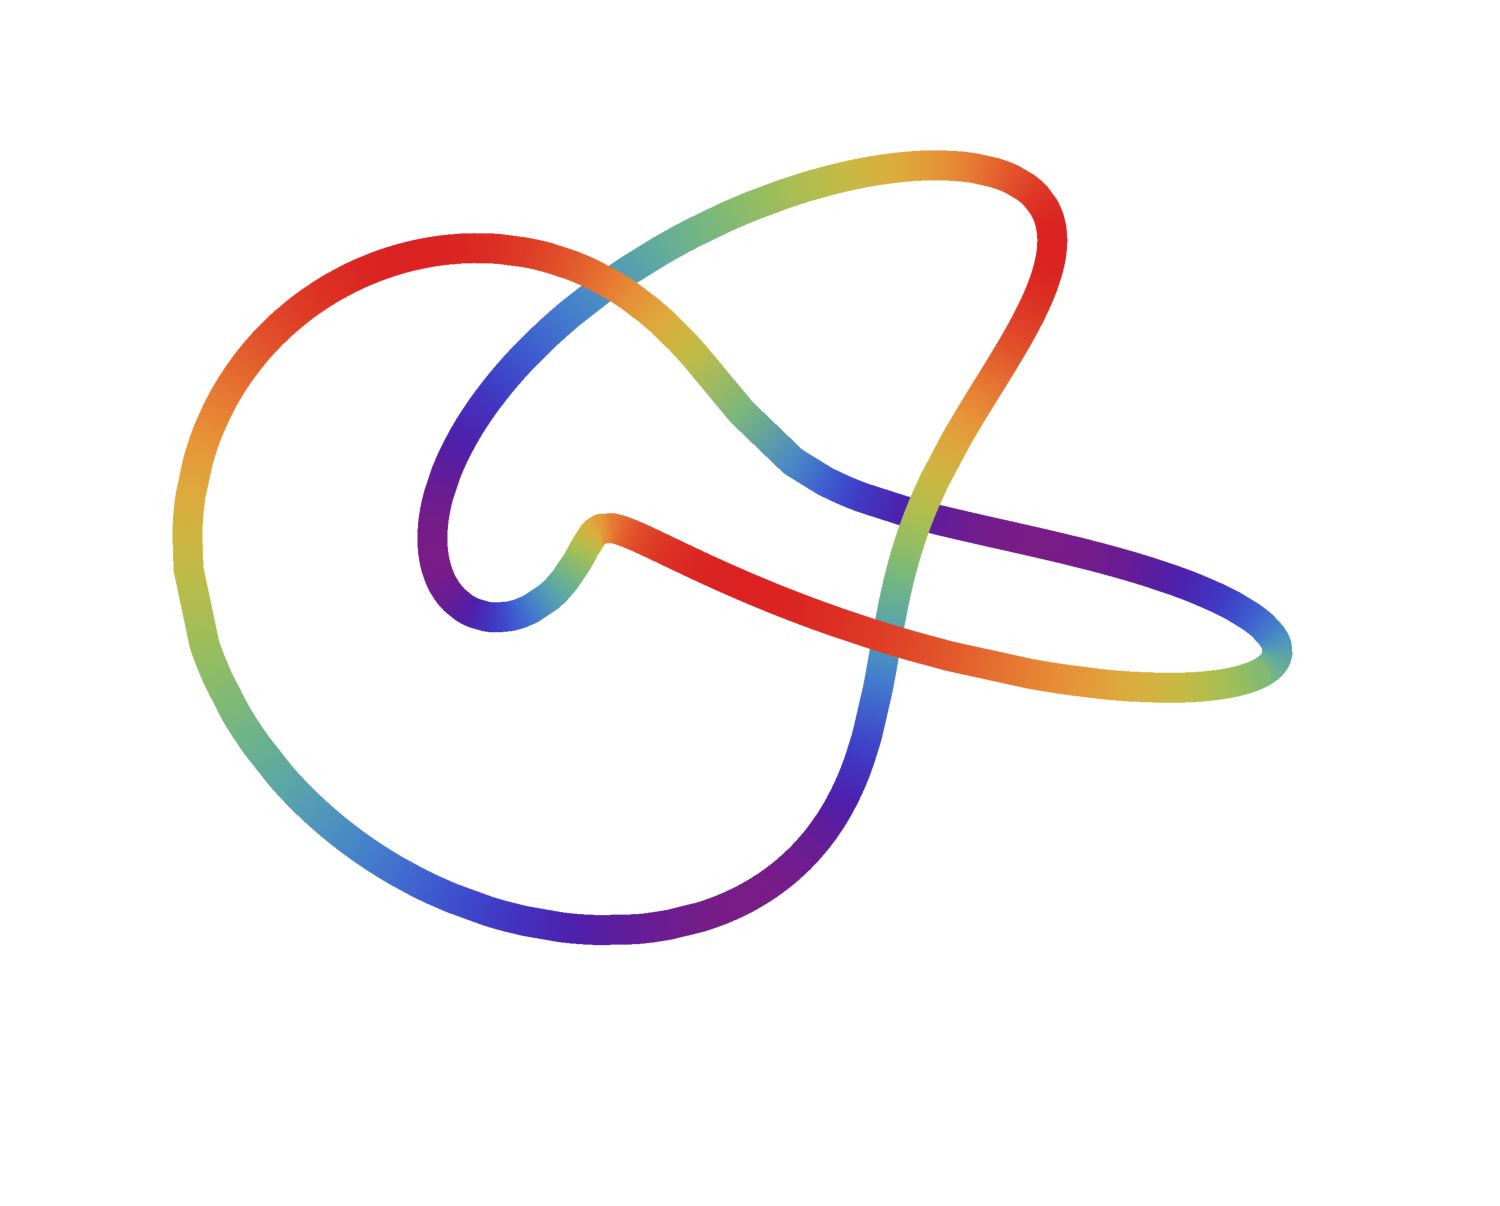
\includegraphics[width=\linewidth]{../data/torus-p2-q3.pdf}
        \subcaption{trójlistnik: $p = 2, q = 3$}
    \end{minipage}
    \begin{minipage}[b]{.3\linewidth}
        \centering
        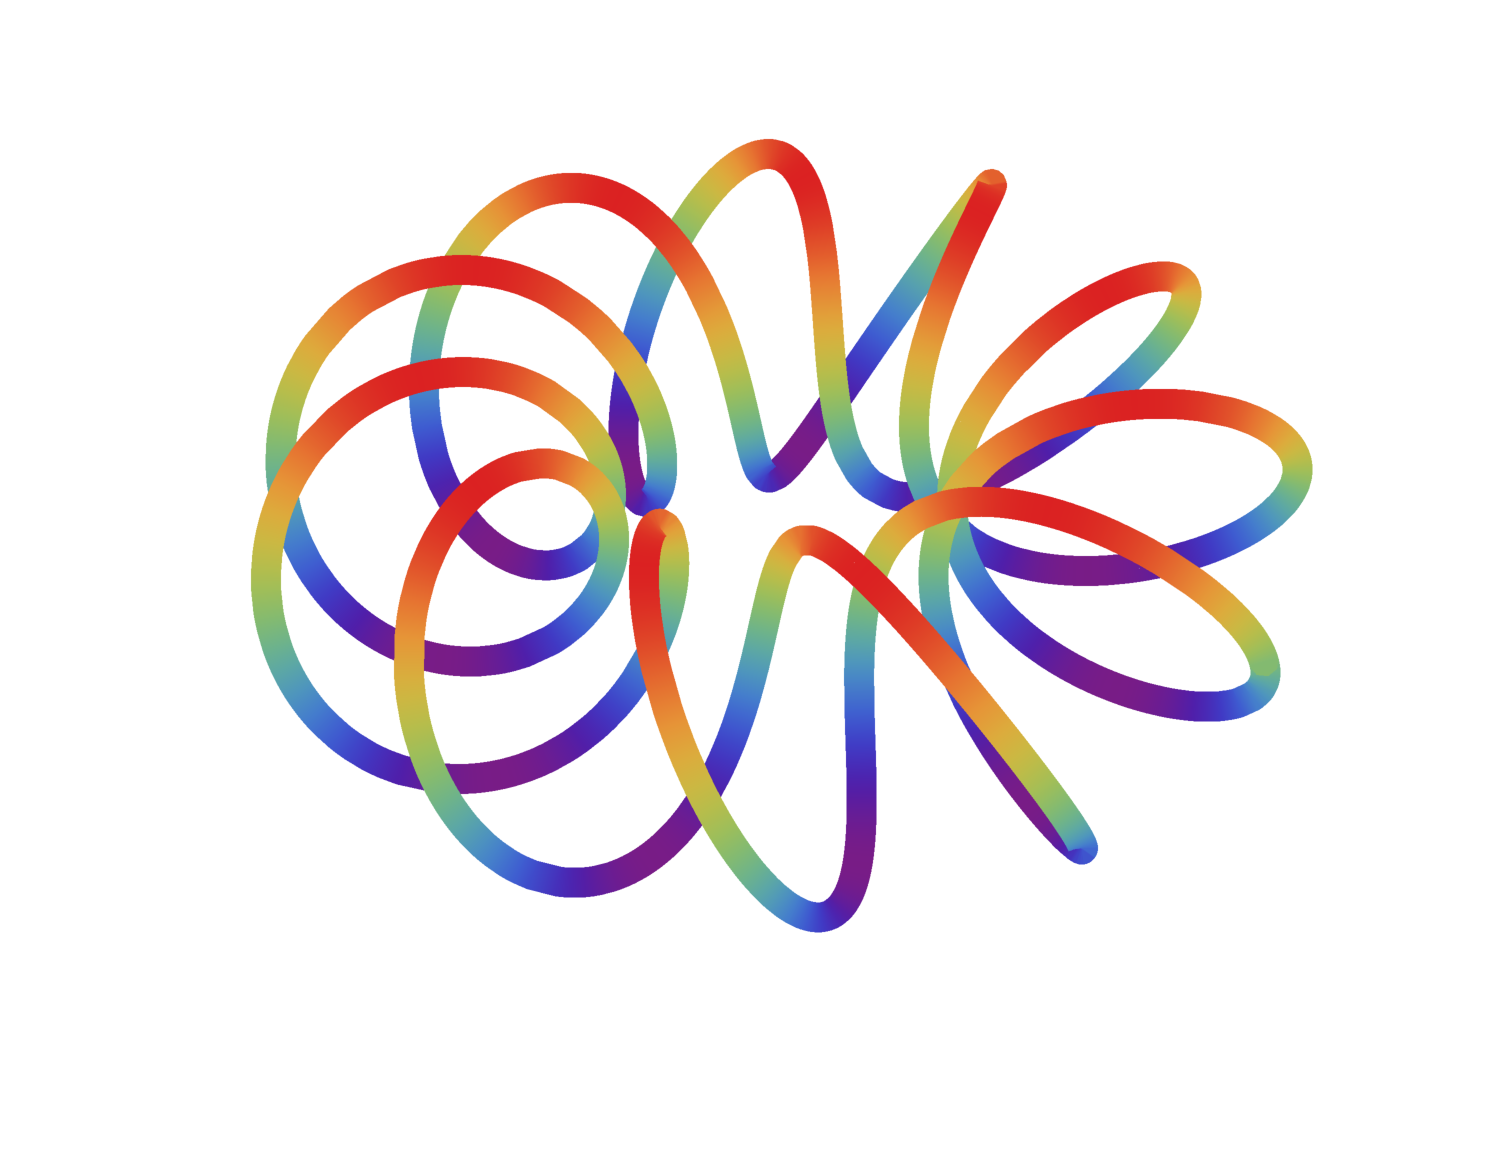
\includegraphics[width=\linewidth]{../data/torus-p2-q11.pdf}
        \subcaption{$p = 2, q = 11$}
    \end{minipage}
    \begin{minipage}[b]{.3\linewidth}
        \centering
        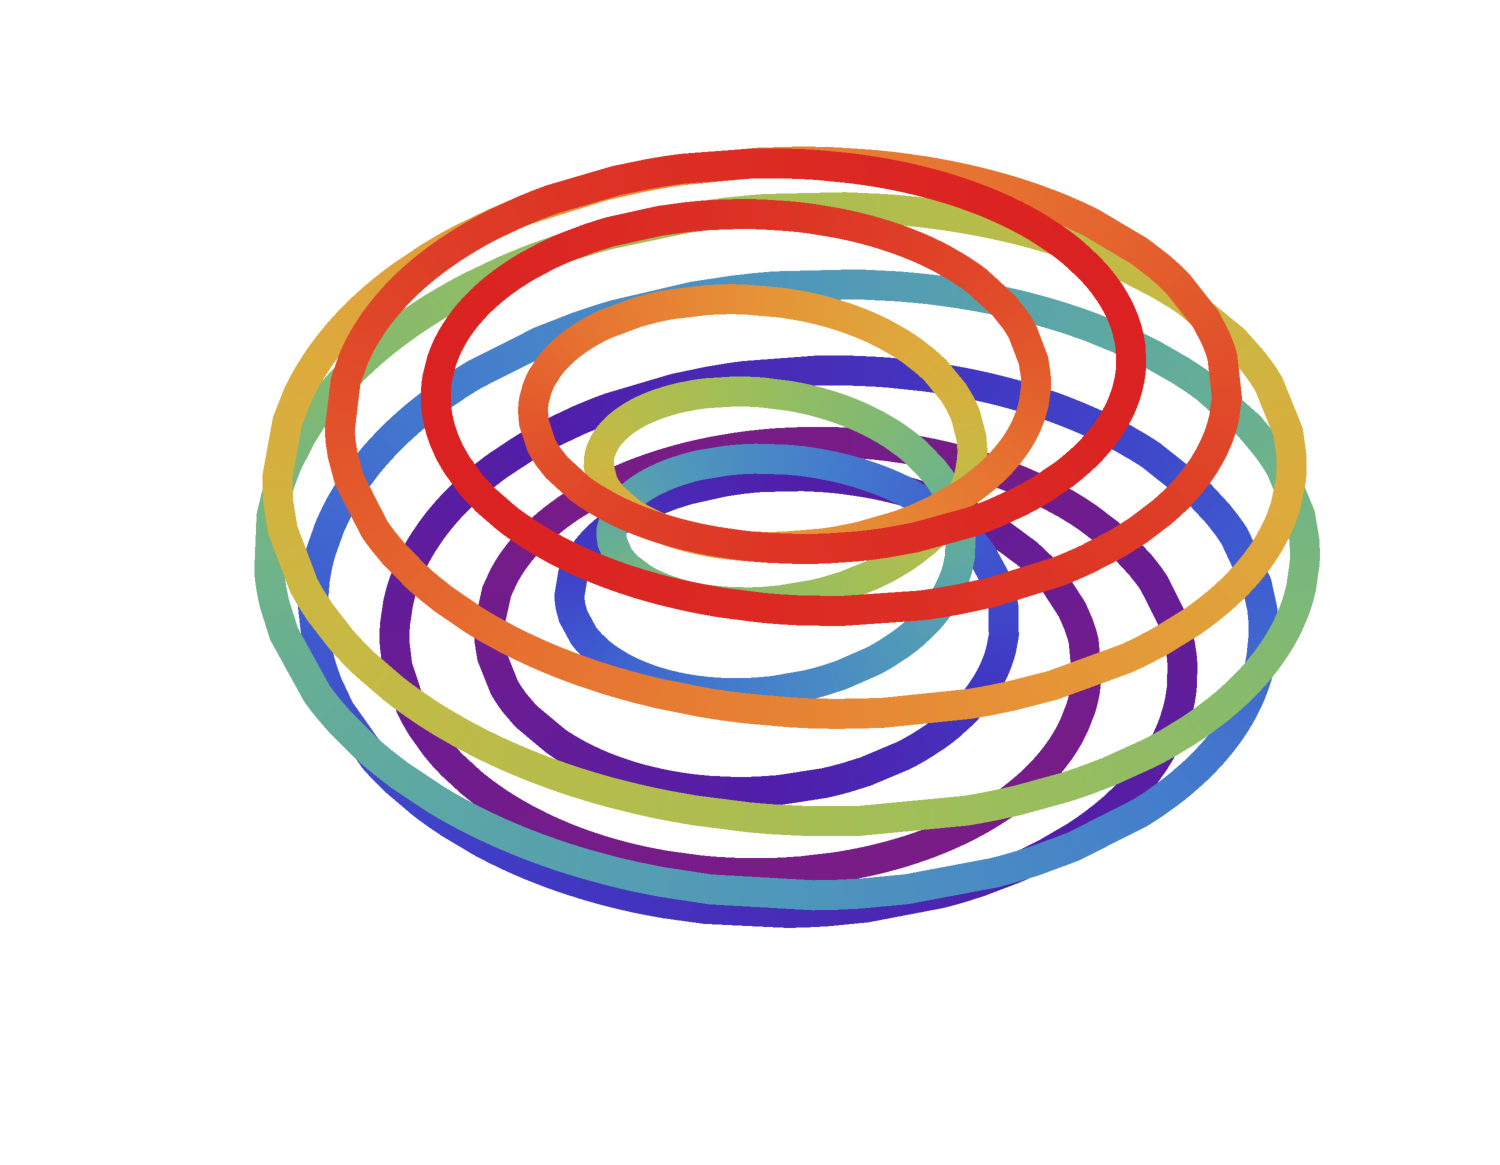
\includegraphics[width=\linewidth]{../data/torus-p11-q2.pdf}
        \subcaption{$p = 11, q = 2$}
    \end{minipage}
\end{figure}

Okazuje się, że innych obiektów już nie ma.

\begin{proposition}
    Jeśli żadna ze składowych splotu torusowego nie jest postaci $K_{0, 0}$ lub $K_{1, 0}$, to splot ten jest równoważny ze splotem $K_{q, r}$ dla pewnych $q, r$.
    Największy wspólny dzielnik indeksów $q, r$ jest jednocześnie liczbą składowych splotu.
\end{proposition}

%Węzeł ten leży na torusie $(r - 2)^2 + z^2 = 1$.
% p = 5;
% q = 3;
% ParametricPlot3D[
% {
% Cos [2 Pi p t] (2 + Cos[2 Pi q t]),
% (2 + Cos[2 Pi q t]) Sin[2 Pi p t],
% -Sin[2 Pi q t]},
% {t, 0, 1},
% ColorFunction -> "Rainbow",
% PlotStyle -> Thickness[0.02],
% Boxed -> False,
% Axes -> False
% ]

Nietrywialne węzły torusowe są pierwsze i odwracalne, ale nie achiralne (mają niezerową sygnaturę).

\begin{proposition}
    Dla $q, r > 0$ zdefiniujmy wielkość $\sigma(q, r) = - \sigma(K_{q, r})$.
    Wtedy, jeśli
    \begin{itemize}[leftmargin=*]
    \itemsep0em
        \item $2r < q$ i $r$ jest parzyste, to $\sigma(q, r) = \sigma(q-2r, r) + r^2$.
        \item $2r < q$ i $r$ jest nieparzyste, to $\sigma(q, r) = \sigma(q-2r, r) + r^2 - 1$.
        \item $\sigma(2r, r) = r^2 - 1$.
        \item jeśli $r \le q < 2r$ i $r$ jest parzyste, to $\sigma(q, r) + \sigma(2r-q, r) = r^2-1$.
        \item jeśli $r \le q < 2r$ i $r$ jest nieparzyste, to $\sigma(q, r) + \sigma(2r-q, r) = r^2-2$.
    \end{itemize}
    Co więcej, $\sigma(q, r) = \sigma(r, q)$, $\sigma(q, 1) = 0$, $\sigma(q, 2) = q-1$.
\end{proposition}

Dowód zawiera praca \cite{litherland81}.

\begin{proposition}
    Ustalmy względnie pierwsze $q, r$ takie, że $|q|, |r| \ge 2$.
    Splot $K(q, r)$ jest równoważny z odwrotnym do niego splotem $K(-q, -r)$.
\end{proposition}

Sploty $K(q, r)$ oraz $K(r, q)$ również są równoważne.
Murasugi prezentuje w książce \cite{murasugi96} przyjemny dowód opierający się na następującym lemacie:
Sfera $S^3$ powstaje z powierzchni dwóch węzłów trywialnych z wnętrzem ($D^2 \times S^1$) przez wzajemne sklejenie południka i równoleżnika z równoleżnikiem i południkiem.

% {\color{red} Longitude, meridian -- ustalić słownictwo}

Macierze Seiferta $M$ mają nieskomplikowaną blokową budowę, która może posłużyć do znalezienia wielomianu Alexandera (wzorem $\Delta = \det (M - tM^t)$).
Rachunki są nieco uciążliwe, oto ich wynik:

\begin{proposition}
    Wielomianem Alexandera splotu torusowego $K(q, r) \neq K(0,0)$ o $d$ składowych jest
    \[
        \Delta_{q, r}(t) = (-1)^{d-1} \frac{(1-t)(1 - t^{qr/d})^d}{(1-t^q)(1-t^r)} \left/t^{(q-1)(r-1)/2}\right. .
    \]
\end{proposition}

Znajomość wielomianu Alexandera wystarcza na szczęście do podania pełnej klasyfikacji węzłów torusowych bez uciążliwego dowodu.

\begin{proposition}
    Węzły torusowe $K(q, r)$, $K(p, s)$ są równoważne wtedy i tylko wtedy, gdy $\{q, r\} = \{p, s\}$ lub $\{q, r\} = \{-p, -s\}$.
\end{proposition}

\begin{proof}
    Ograniczymy się do przypadku, gdy $p, q, r, s \ge 2$.
    Tylko jedna implikacja wymaga dowodu, w prawo.
    Bez straty ogólności załóżmy więc, że $q > r$, $p > s$.
    Skoro węzły $K(q, r)$ i $K(p,s)$ są równoważne, to porównanie najwyższych współczynników w ich wielomianach Alexandera daje równość $(q-1)(r-1) = (p-1)(s-1)$.
    Wymnożenie wszystkiego prowadzi do czterech przypadków: $s = r$, $s = ps$, $qr = r$, $qr = ps$, z których dwa środkowe nie mogą zachodzić (gdyż $p, q > 1$).
    Z czwartego wynika, że $qr \le s < ps$, czyli sprzeczność.
\end{proof}

Podamy teraz wartości całkowitoliczbowych niezmienników dla węzłów torusowych przy założeniu, że $q$ lub $r$ nie jest zerem.

\begin{proposition}[Murasugi, 1991]
    Mamy $cr(K_{q,r}) = \min\{|q|(|r| -1), |r|(|q|-1)\}$.
\end{proposition}

Wyznaczenie indeksu rozwiązującego było dużo trudniejsze.
Murasugi pisze w książce \cite{murasugi96}, że mamy nierówność
\[
    u(K(q, r)) \le \frac 12 (q-1)(r-1),
\]
z równością dla względnie pierwszych $q, r > 0$.
Hipoteza Milnora głosiła, że w rzeczywistości równość zachodzi zawsze.
Dowód został odnaleziony w latach 1993-1995 przy użyciu tzw. \emph{gauge theory} (działu teorii pola, gdzie lagranżjan jest niezmienniczy względem grup Liego lokalnych transformacji...)

\begin{proposition}[Kronheimer, Mrówka] \label{torus_unknotting}
    Mamy
    \[
        u(K(q, r)) = \frac 12 (q-1)(r-1),
    \]
\end{proposition}

Genus pokrywa się z liczbą gordyjską dla węzłów (czyli względnie pierwszych $q, r$).

\begin{proposition} \label{torus_bridge}
    Mamy $br(K_{q,r}) = \min \{|q|, |r|\}$.
\end{proposition}

\begin{proposition}
    Mamy $\bracket{K_{2, n}} = A \bracket{K_{2,n-1}} + (-1)^{n-1} A^{2-3n}$
    oraz $\bracket{K_{2,1}} = -A^3$.
\end{proposition}

\begin{proposition}
    Wielomianem Jonesa węzła $(m, n)$-torusowego jest
    \[
        V(t) = \frac {t^{(m-1)(n-1):2}}{1-t^2} \cdot (1 - t^{m+1} - t^{n+1} + t^{m+n}).
    \]
\end{proposition}

Murasugi i Neuwirth w 1961 dla węzłów alternujących,
zaś Burde z Zieschangiem w 1965 pokazali, że nietrywialny węzeł,
którego grupa ma nietrywialne centrum, jest torusowy.

\begin{proposition}
    Wielomianem Alexandera węzła $(p,q)$-torusowego jest
    \[
         \Delta(T_{p,q}) = \frac{(t^{pq}-1)(t-1)}{(t^p-1)(t^q-1)}.
    \]
\end{proposition}

\begin{proof}
    Przypadek $p = 2$ wymaga prostego rozumowania indukcyjnego.
    Samo ćwiczenie pojawia się w wielu podręcznikach topologii.
    Pełny dowód można znaleźć w przykładzie 9.15 książki ,,Knots'' Burdego oraz Zieschanga.
    Inne podejście, tak zwaną formułę Seiferta-Torresa, prezentuje przeglądowa praca Turaewa ,,Reidemeister torsion in knot theory'', 119-182.
\end{proof}

\begin{corollary}
    Wielomian Alexandera odróżnia od siebie węzły $(2,n)$-torusowe.
\end{corollary}

\begin{proof}
    Mamy $\Delta(T_{2,n}) = (t^n+1) / (t+1)$, więc $\deg \Delta (T_{2,n}) = n - 1$.
\end{proof}

% Koniec sekcji Węzły torusowe

\section{Węzły satelitarne} % (fold)
\label{sec:satellite}
Wyobraźmy sobie węzeł $K'$ leżący wewnątrz trywialnego torusa $V$ tak, by nie zawierał się w żadnej mieszczącej się w tym torusie 3-kuli.
Zawiążmy następnie torus $V$: ustalmy włożenie $f \colon V \to S^3$.
Splot $K = f(K')$ orbituje wokół swojego kompana, tj. obrazu rdzenia torusa przez włożenie $f$ i nie opuszcza jego małego rurowego otoczenia.
Dość nieprzypadkowo splot $K$ nazywamy satelitarnym, zaś obraz rdzenia -- węzłem towarzyszącym.
Konstrukcja satelity jest, w porównaniu z sumą spójną, dość zawiła.
Pożądanym byłoby mieć do dyspozycji więcej operacji rozkładających węzły na prostsze, i badać nierozkładalne obiekty.
Ale ich nie ma.

Torus $f(\partial V)$ nie jest równoległy do brzegu ani ściśliwy.
Odwrotnie, jeśli w dopełnieniu węzła mamy torus, którego południk lub równoleżnik ogranicza dysk, to węzeł nie biegnie wzdłuż torusa lub ten jest niezawęźlony.
Przypadek, gdy torus jest otoczeniem rurowym węzła, też nie jest ciekawy.
To motywuje następującą definicję.

\begin{definition}
	\index{węzeł!satelitarny}
	Węzeł nazywamy satelitarnym, jeśli zawiera nieściśliwy, nierównoległy do brzegu torus we własnym dopełnieniu.
\end{definition}

Klasa węzłów satelitarnych obejmuje węzły złożone.
W ich przypadku można wskazać pewien szczególny torus nieściśliwy -- połykający pierwszy składnik, a potem podążający za drugim.
Świetnie przedstawione jest to na stronie 82 książki \cite{cromwell04} Cromwella.
Niektóre węzły przedstawiają się jako satelity w dokładnie jeden sposób, inne nie są jednoznaczne.
W \cite{jaco79} ulepszono definicję satelitarności do tzw. \emph{splicing}u i opisano jednoznaczny rozkład Jaco-Shalena-Johannsona, czego prawdziwość przypuszczał wcześniej Waldhausen.
Żaden węzeł torusowy ani trywialny nie jest satelitą, ale są nimi kable oraz duble Whiteheada.

\begin{definition}
	\index{dubel Whiteheada}
	Jeżeli $K' \subseteq V$ jest skręconym jednokrotnie niewęzłem, to węzeł $K$ nazywamy dublem Whiteheada.
\end{definition}

Każdy węzeł posiada nieskończenie wiele dubli Whiteheada: wystarczy rozciąć torus $V$, skręcić jedną końcówkę i ponownie zszyć, żaden z nich nie jest odróżniany od niewęzła przez wielomian Alexandera.

\begin{definition}
	\index{węzeł!kablowy}
	Jeżeli $K' \subseteq \partial V$ jest węzłem torusowym,	to $K$ nazywamy węzłem kablowym.
\end{definition}

Satelita, którego indeks zawijający przekracza dwa, ma co najmniej 27 skrzyżowań.
Jeśli jego kompan to ósemka -- co najmniej siedemnaście.
Oprócz tego istnieją cztery satelity o ponad dwunastu skrzyżowaniach.
Podejrzewa się, że satelita, który wykonuje $m$ pełnych obrotów wokół kompana o indeksie skrzyżowaniowym $k$, nie posiada diagramu o mniej niż $km^2$ skrzyżowaniach.

\begin{proposition}
	Każdy kabel wyznacza jednoznacznie węzeł, z którego powstał.
\end{proposition}

\begin{proof}
	Wniosek 2 z pracy \cite{feustel78} Feustela, Whittena pokazuje, że na podstawie kabla można wyznaczyć parametry węzła torusowego $K'_{p,q}$ oraz topologię dopełnienia oryginalnego węzła.
	Wiemy jednak z twierdzenia Gordona-Lueckego, że różne węzły mają różne dopełnienia.
\end{proof}

Schubert pokazał, że zorientowane klasy izotopii węzłów w $S^3$ tworzą wolny przemienny monoid na przeliczalnie wielu generatorach.
Krótko po tym odkrył, że może podać nowy dowód tego twierdzenia przez uważną analizę nieściśliwych torusów obecnych w dopełnieniu sumy spójnej.
To doprowadziło go do definicji węzłów satelitarnych i towarzyszących w przełomowej pracy \cite{schubert53} oraz zunifikowało teorię 3-rozmaitości oraz węzłów.
Patrz też \cite{motegi97}.

% Koniec sekcji Węzły satelitarne

\section{Węzły hiperboliczne} % (fold)
\label{sec:hyperbolic}
\begin{definition}
    Węzeł nazywamy hiperbolicznym, jeżeli na jego dopełnieniu można zadać metrykę o~stałej krzywiźnie $-1$.
    \index{węzeł!hiperboliczny}
\end{definition}

\begin{theorem}[trychotomia Thurstona, 1978]
    \index{twierdzenie!Thurstona}
    Każdy węzeł należy do dokładnie jednej z trzech nieskończonych rodzin: węzłów torusowych, satelitarnych albo hiperbolicznych.
\end{theorem}

% Stwierdzenie to nazywa się czasem trychotomią Thurstona, gdyż dzieli węzły na trzy rodzaje.
Z twierdzenia o~sztywności (\emph{rigidity theorem}) Mostowa i~Prasada (1973), jeśli na dopełnieniu węzła można zadać strukturę hiperboliczną, to w~tylko jeden sposób.
\index{twierdzenie!o sztywności}
Co więcej, Mostow pokazał, że jeśli istnieje izomorfizm grup podstawowych domkniętych, hiperbolicznych 3-rozmaitości, to są one izometryczne.
Wiedzę o~węzłach hiperbolicznych można czerpać z~prac: \cite{weeks05} (poprawiona wersja dostępna w~serwisie ArXiv), "Hyperbolic Knot Theory" J. Purcell.

\begin{proposition}[kryterium Thurstona]
    Niech $L$ będzie splotem z dopełnieniem $X$ i grupą podstawową $\pi = \pi_1(X)$.
    Jeżeli spełnione są następujące warunki:
    \begin{enumerate}
    \item $L$ nie rozszczepia się,
    \item $L$ nie jest niewęzłem,
    \item żadna składowa $L$ nie jest niezakłóconym węzłem satelitarnym (?),
    \item $L$ nie jest węzłem torusowym,
    \end{enumerate}
    to $L$ jest splotem hiperbolicznym.
    Warunki podane wyżej mają swoje odpowiedniki dla przestrzeni $X$ ($X$ nie zawiera właściwej 2-sfery, właściwego dysku, właściwego torusa, właściwego pierścienia) oraz grupy $\pi$ ($\pi$ nie jest wolnym produktem, nie jest cykliczna oraz nie zawiera kopii $\Z^2$).
\end{proposition}

\begin{proposition}
    Żaden węzeł nie ma mniejszej objętości hiperbolicznej od ósemki.
\end{proposition}

Dowód tego faktu podał Cao z~Meyerhoffem w~2001 roku.
Opierali się oni na działaniu komputerowego programu, który wyeliminował inne możliwości.

\begin{proposition}
    Objętość hiperboliczna nie odróżnia hiperbolicznych mutantów.
\end{proposition}

Nie jestem w~stanie podać odnośnika do dowodu w~literaturze -- przypominam, że chodzi o~mutanty z~definicji \ref{def:mutant}.
Stwierdzenie to można znaleźć na przykład w~książce Adamsa (strona 124).

\begin{proposition}
    Grupa symetrii węzła hiperbolicznego jest skończona: cykliczna lub diedralna.
\end{proposition}

\begin{proof}
    Praca \cite{kodama92}.
\end{proof}

Objętość hiperboliczna bardzo dobrze odróżnia od siebie węzły.
Pewien węzeł o~dwunastu skrzyżowaniach i~$5_2$ mają jednak tę samą objętość.

\begin{proposition}
    Każdy węzeł hiperboliczny jest pierwszy.
\end{proposition}

Prawie każdy węzeł pierwszy o~mniej niż 17 skrzyżowaniach jest hiperboliczny, na 32 wyjątki składa się 12 węzłów torusowych oraz 20 satelitów trójlistnika.
Te ostatnie mają co najmniej 11 skrzyżowań.
Baza ciągów liczb całkowitych OEIS zawiera informacje na temat liczności poszczególnych typów węzłów.
Analizując ciągi A051764, A051765 oraz A052408 można dojść do wniosku, że wraz ze wzrostem liczby skrzyżowań, stosunek liczby węzłów hiperbolicznych do wszystkich węzłów dąży do $1$:

\renewcommand*{\arraystretch}{1.4}
\footnotesize
\begin{longtable}{lcccccccccccccc}
\hline
    \textbf{rodzaj} & 3 & 4 & 5 & 6 & 7 & 8  & 9  & 10  & 11  & 12   & 13   & 14    & 15     \\ \hline \endhead
    torusowe        & 1 & 0 & 1 & 0 & 1 & 1  & 1  & 1   & 1   & 0    & 1    & 1     & 2      \\
    satelitarne     & 0 & 0 & 0 & 0 & 0 & 0  & 0  & 0   & 0   & 0    & 2    & 2     & 6      \\
    hiperboliczne   & 0 & 1 & 1 & 3 & 6 & 20 & 48 & 164 & 551 & 2176 & 9985 & 46969 & 253285 \\
    \hline
\end{longtable}
\normalsize

W pracy \cite{malyutin16} A. Malyutin pokazał jednak, że to przypuszczenie jest sprzeczne z~wieloma innymi starymi hipotezami teorii węzłów: \ref{malyutin1} -- \ref{malyutin4}.

\begin{conjecture}
    \label{malyutin1}
    Indeks skrzyżowaniowy jest addytywny względem sumy spójnej.
\end{conjecture}

(To jest powtórzenie hipotezy \ref{cnj:crossing_additive}).
Murasugi dowiódł prawdziwości hipotezy dla węzłów alternujących, w~pracy \cite{murasugi87} jest to wniosek z~dowodu hipotezy Taita.
Krótko po tym Lickorish, Thistlethwaite powtórzyli to dla węzłów adekwatnych w \cite{lickorish88}.
Na początku XX wieku Diao \cite{diao04} oraz Gruber \cite{gruber03} niezależnie udowodnili hipotezę \ref{malyutin1} dla pewnej szerokiej klasy węzłów, obejmującej wszystkie węzły torusowe oraz wiele węzłów alternujących oraz pewne inne obiekty, których nie chcemy opisywać.

\begin{conjecture}
    Satelita ma większy (w słabszej wersji: nie mniejszy) indeks skrzyżowaniowy niż jego towarzysze.
\end{conjecture}

Lackenby pokazał w~\cite{lackenby14}, że jeśli $K$ jest satelitą z towarzyszem $L$, to $\operatorname{cr} K \ge 10^{-13} \operatorname{cr} L$.

\begin{conjecture}
    Węzeł złożony ma większy (w słabszej wersji: nie mniejszy) indeks skrzyżowaniowy niż jego faktory.
\end{conjecture}

Mówimy, że węzeł pierwszy $P$ jest $\lambda$-regularny, jeśli $cr K \ge \lambda \cdot cr P$ za każdym razem, gdy węzeł $P$ jest faktorem węzła $K$.
Zatem hipotezę można wysłowić krótko ,,węzły pierwsze są $1$-regularne''.
Na podstawie prac Murasugiego, Kauffmana i~Thistlethwaite'a z~końca lat 80. wiemy, że zachodzi dla węzłów alternujących.
Diao pokazał w \cite[tw. 3.8]{diao04}, że węzły torusowe także są $1$-regularne, natomiast Lackenby przedstawił w~\cite{lackenby09} rozumowanie, dlaczego wszystkie węzły są $1/152$-regularne.
Pisaliśmy o tym w podsekcji \ref{sub:crossing_number}.

\begin{conjecture}
    \label{malyutin4}
    Węzły pierwsze są $2/3$-regularne.
\end{conjecture}

Rozwiązanie zagadki przyniosła praca samego Malyutina \cite{malyutin19} opublikowana latem 2019 roku, przynajmniej dla splotów.
Pokazał w~niej, że jeśli oznaczymy liczbę splotów pierwszych i~nierozszczepialnych o~$n$ lub mniej skrzyżowaniach przez $P_n$, zaś liczbę hiperbolicznych splotów, także o~$n$ lub mniej skrzyżowaniach, przez $H_n$, prawdziwe będzie oszacowanie
\begin{equation}
    \liminf_{n \to \infty} \frac{H_n}{P_n} < 1 - 10^{-13}.
\end{equation}

% Every non-split, prime, alternating link that is not a~torus link is hyperbolic by a~result of William Menasco.



% https://arxiv.org/abs/math/0309466
% https://arxiv.org/abs/math/0311380
% Koniec sekcji Węzły hiperboliczne

\section{Węzły plastrowe i taśmowe}
\label{sec:slice}
Węzły plastrowe i taśmowe oraz pojęcie kobordyzmu, które wkrótce opiszemy, należą do świata 4-wymiarowej teorii węzłów.
Nie zapoznamy się z nią bliżej oraz nie podamy naszego ulubionego odniesienia do tego tematu w~literaturze, ponieważ sami nie rozumiemy go zbyt dobrze.
Wszystko zaczęło się od artykułu \cite{fox66} Foxa, Milnora.

%%% Kawauchi 155:

\begin{definition}[płaski dysk]
    Niech $D \subseteq B^4$ będzie dyskiem posiadającym otoczenie $N$, kopię zbioru $D \times I^2$, która przecina sferę $S^3$ dokładnie w $\partial D \times I^2$.
    Mówimy wtedy, że dysk $D$ jest płaski.
\end{definition}

\begin{tobedone}
    Płaski? Lokalnie płaski?
    \cite[s. 155]{kawauchi96}
\end{tobedone}

\begin{definition}[węzeł plastrowy]
    \index{węzeł!plastrowy}
    Niech $K \subseteq S^3$ będzie takim węzłem, że w kuli $B^4$ istnieje płaski dysk $D$ taki, że $K = \partial D = D \cap S^3$.
    Wtedy $K$ nazywamy węzłem plastrowym.
\end{definition}

Następujące węzły o~mniej niż jedenastu skrzyżowaniach są plastrowe: $6_1$, $8_{8}$, $8_{9}$, $8_{20}$, $9_{27}$, $9_{41}$, $9_{46}$, $10_{3}$, $10_{22}$, $10_{35}$, $10_{42}$, $10_{48}$, $10_{75}$, $10_{87}$, $10_{99}$, $10_{123}$, $10_{129}$, $10_{137}$, $10_{140}$, $10_{153}$ oraz $10_{155}$.
\index{węzeł!Conwaya}
Wśród pierwszych węzłów do dwunastu skrzyżowań najdłużej opierał się węzeł Conwaya, aż Piccirillo pokazała w~\cite{piccirillo20}, że nie jest plastrowy.

\begin{proposition}
    Niech $K$ będzie węzłem.
    Wtedy $K \shrap mr K$ jest węzłem plastrowym.
\end{proposition}

\begin{proof}[Niedowód]
    Pierwszy był Fox z Milnorem \cite{fox66}, patrz także lemat 12.1.2.2 w \cite{kawauchi96}.
\end{proof}

\begin{proposition}
    Albo wszystkie trzy węzły $K_1, K_2, K_1 \shrap K_2$ są plastrowe, albo co najwyżej jeden z~nich.
\end{proposition}

\begin{proof}[Niedowód]
    Lemat 12.1.2.3 w \cite{kawauchi96}.
\end{proof}

Pierwszym poważnym wynikiem z dziedziny teorii węzłów plastrowych, pochodzącym jeszcze z pracy \cite{fox66}, był:

\begin{proposition}[warunek Foxa-Milnora]
    \index{warunek!Foxa-Milnora}
    Niech $K$ będzie węzłem plastrowym.
    Wtedy jego wielomian Alexandera jest postaci $\alexander(t) = f(t) f(1/t)$ dla pewnego wielomianu Laurenta $f \in \Z[t, 1/t]$.
\end{proposition}

\begin{corollary}
    \index{wyznacznik}
    Wyznacznik węzła plastrowego jest kwadratem.
\end{corollary}

\begin{proof}
    Mamy $\det K = |\alexander(-1)| = f(-1) f(-1)$.
\end{proof}

Ten prosty test stwierdza, że 2743 spośród 2977 węzłów o mniej niż 13 skrzyżowaniach nie jest plastrowych.

\begin{proposition}
    \index{sygnatura}
    \label{prp:slice_signature}
    Niech $K$ będzie węzłem plastrowym.
    Wtedy $\sigma(K) = 0$.
\end{proposition}

\begin{tobedone}[Szkic dowodu]
    Ustalmy odwzorowanie $f$, które jest niesingularne, symetryczne i~dwuliniowe, z~przestrzeni $V$ o~wymiarze $2n$ oraz wyznaczoną przez nie formę kwadratową.
    Jeśli znika ona na podprzestrzeni wymiaru $n$, to ma zerową sygnaturę.
    dowód znaleziony w~podręczniku Lickorisha.
    Patrz też twierdzenie 8.8 z~artykułu \cite{murasugi65}.
    Praca "Infinite Order Amphicheiral Knots". (Charles Livingston, 2001) -- chyba nie?
\end{tobedone}

Test ten eliminuje kolejne 45 węzłów poniżej 13 skrzyżowań.

\begin{proposition}
    \index{niezmiennik!Arfa}
    Niech $K$ będzie węzłem plastrowym.
    Wtedy $\operatorname{Arf} K = 0$.
\end{proposition}

\begin{proof}
    Ustalmy węzeł $K$, wiemy już, że jego wyznacznik jest kwadratem, a na mocy faktu \ref{cor:knot_determinant_odd} także tyle, że jest liczbą nieparzystą.
    Wynika stąd przystawanie $\det K \equiv 1 \mod 8$, które w~połączeniu z warunkiem Murasugiego (fakt \ref{prp:arf_murasugi}) daje $\operatorname{Arf} K = 0$.
\end{proof}

\begin{proposition}
    Niech $K$ będzie węzłem w kategorii TOP.
    Jeżeli jego wielomian Alexandera jest trywialny: $\alexander_K(t) \equiv 1$, to węzeł $K$ jest plastrowy.
\end{proposition}

\begin{proof}
    Freedman w \cite[tw. 1.13]{freedman82}.
\end{proof}

Jak wynika z twierdzenia Donaldsona, wynik przestaje być prawdziwy po przejściu kategorii PL.
Dość klarownie różnicę między tymi dwiema kategoriami tłumaczy Gompf w~\cite{gompf86}.  

%%% Kawauchi 156:
\subsection{Zgodność}
Wprowadzimy teraz relację równoważności na zbiorze węzłów, która prowadzi przez fakt \ref{prp:cobordant_iff_sum_slice} do alternatywnej definicji węzłów plastrowych.

\begin{definition}[zgodność]
    \index{kobordyzm}
    \index{zgodność}
    % Dwa węzły $K_0, K_1$ takie, że istnieje lokalnie płaski, zorientowany, właściwy pierścień $C$ taki, że $C \cap S^3 \times i = K_i \times i$, nazywamy zgodnymi.
    % Dwa sploty $K, L \subseteq S^n$ nazywamy zgodnymi (z angielskiego \emph{concordant}), jeśli istnieje włożenie $f \colon K \times [0,1] \to S^n \times [0,1]$ spełniające dwa warunki: $f(K \times 0) = K \times 0$ oraz $f(K \times 1) = L \times 1$.
    Dwa węzły $K_0, K_1$ nazywamy (gładko) zgodnymi, jeżeli istnieje gładko zanurzony pierścień w $S^3 \times I$, którego brzegiem jest zbiór $K_0 \times 0 \cup K_1 \times 1$.
        % z \cite{gompf86}
\end{definition}

W języku angielskim przez zgodność rozumie się zazwyczaj \emph{concordance}, rzadziej termin \emph{cobordism}.

\begin{proposition}
    \label{prp:cobordant_iff_sum_slice}
    Dwa węzły $K_1, K_2$ są zgodne wtedy i tylko wtedy, gdy suma $mr K_0 \shrap K_1$ jest plastrowa.
\end{proposition}

\begin{proof}
    Ćwiczenie 12.1.3 w \cite{kawauchi96}.
\end{proof}

\begin{definition}
    Węzeł zgodny z~niewęzłem nazywamy plastrowym.
\end{definition}

,,Bycie zgodnym'' jest relacją równoważności, słabszą od bycia izotopijnym.
% ale mocniejszą od homotopii?
% izotopia: https://encyclopediaofmath.org/wiki/Cobordism_of_knots
Klasę abstrakcji węzła $K$ oznaczamy przez $[K]$.

\begin{definition}[grupa zgodności]
    \index{grupa!zgodności}
    Niech $C^1$ oznacza iloraz zbioru wszystkich węzłów przez relację zgodności.
    Zbiór $C^1$ wyposażony w~działanie
    \begin{equation}
        [K_1] + [K_2] = [K_1 \shrap K_2]
    \end{equation}
    staje się grupą abelową, nazywaną grupą zgodności.
    Jej elementem eneutralnym jest klasa abstrakcji niewęzła.
    Elementem przeciwnym do $[K]$ jest $[mr K]$.
\end{definition}

%%% Kawauchi 157:

Niech $\Theta$ oznacza rodzinę macierzy Seiferta, kwadratowych macierzy $V$ o całkowitych wyrazach takich, że $\det (V - V^T) = 1$.
Mówimy, macierz $V \in \Theta$ jest zerowo kobordantna, jeśli istnieje całkowitoliczbowa macierz $P$ o~wyznaczniku równym $\pm 1$, że
\begin{equation}
    V = P \begin{pmatrix} 0 & V_{21} \\ V_{12} & V_{22} \end{pmatrix} P^{-1}
\end{equation}
\index{macierz!unimodularnie sprzężona}
Takie macierze nazywamy unimodularnie sprzężonymi.

\begin{proposition}
    Niech $V \in \Theta$ będzie macierzą zerowo kobordantną.
    Wtedy istnieje plastrowy węzeł $K$, którego macierzą Seiferta jest $V$.
\end{proposition}

\begin{proof}
    Fakt 12.2.1 w \cite{kawauchi96}.
\end{proof}

Przez analogię, o dwóch macierzach $V_1, V_2 \in \Theta$ mówimy, że są kobordantne, jeżeli $(-V_1) \oplus V_2$ jest zerowo kobordantna.
Kobordyzm jest znowu relacją równoważności, iloraz $\Theta$ przez nią oznaczamy przez $G_-$, a elementy tego ilorazu jako $[V]$.
Wyposażony w działanie $[V_1] + [V_2] = [V_1 \oplus V_2]$ staje się grupą abelową.

\begin{proposition}
    % Kawauchi 12.2.8
    Odwzorowanie $\psi \colon C^1 \to G_-$ posyłające klasę abstrakcji węzła w klasę abstrakcji jego macierzy Seiferta jest dobrze określonym epimorfizmem.
\end{proposition}

\begin{proof}
    Funkcja $\psi$ jest dobrze określona na mocy faktu \ref{prp:cobordant_to_algebraic_is_algebraic}, jest homomorfizmem jak wynika z dowodu faktu \ref{prp:signature_additive}.
    To, że jest ,,na'', jest wnioskiem z \cite[s. 62]{kawauchi96}
\end{proof}

Funkcję $\psi$ rozpatrywał Levine \cite{levine69}.
Casson, Gordon pokazali w latach 70., że jej jądro jest niepuste \cite{gordon78}.

\begin{proposition}
    % Dowód tego faktu jest pominięty nawet w pracy Kawauchiego
    $G_- \cong \Z^\infty \oplus (\Z/4\Z)^\infty \oplus (\Z/2\Z)^\infty$.
    % TODO: (Livingston: A SURVEY OF CLASSICAL KNOT CONCORDANCE)
    % The application of abelian knot invariants (those determined by the cohomology of abelian covers or, equivalently, by the Seifert form) to concordance culminated in 1969 with Levine’s classification of higher dimensional knot concordance, [62, 63], which applied in the classical dimension to give a surjective homomorphism $\varphi \colon C \to \Z^\infty \oplus \Z_2^\infty \oplus \Z_4^\infty$.
    % In 1975 Casson and Gordon [8, 9] proved that Levine’s homomorphism is not an isomorphism, constructing nontrivial elements in the kernel, and Jiang expanded on this to show that the kernel contains a subgroup isomorphic to $\Z_2^\infty$. 
\end{proposition}


\subsection{Węzły taśmowe}
\begin{definition}
    \index{węzeł!taśmowy}
    Węzeł $K = f(S^1)$ będący brzegiem singularnego dysku $f \colon D \to S^3$ posiadającego następującą własność: każda przecinająca siebie składowa jest łukiem $A \subseteq f(D^2)$, dla którego $f^{-1}(A)$ składa się z~dwóch łuków w~$D^2$ (jeden z~nich jest wewnętrzny), nazywamy taśmowym.
\end{definition}

Jak pisze Kawauchi, mamy oczywiste wynikanie:

\begin{proposition}
    Każdy węzeł taśmowy jest plastrowy.
\end{proposition}

Dawno temu Fox zapytał, czy implikacja odwrotna także jest prawdziwa:

\begin{conjecture}[slice-ribbon problem]
    \index{hipoteza!plastrowo-taśmowa}
    Czy każdy węzeł plastrowy jest taśmowy?
\end{conjecture}

Nie wiemy do dzisiaj.
Lisca pokazał prawdziwość hipotezy dla węzłów 2-mostowych \cite{lisca07}, Greene oraz Jabuka zrobili to dla precli o trzech pasmach w \cite{greene11}.
\index{węzeł!2-mostowy}
\index{węzeł!preclowy}
P. Teichner myśli o niej jako o~życzeniu, które uprościłoby pewne 4-wymiarowe problemy, gdyby było prawdziwe, ale Gompf, Scharlemann i Thompson zasugerowali w~\cite{gompf10} potencjalny kontrprzykład.

\subsection{Węzły skręcone}
\begin{definition}
    \index{węzeł!skręcony}
    \label{def:twist_knot}
    Węzeł powstały przez $n$-krotne półskręcanie domkniętej pętli oraz splecienie końców nazywamy węzłem skręconym.
\end{definition}

Węzły skręcone to dokładnie towarzyszące niewęzłowi w~węzłach satelitarnych, tak zwane whiteheadowskie duble niewęzła.
Wszystkie są odwracalne (ale tylko niewęzeł oraz ósemka są amfichiralne) i~mają liczbę gordyjską $1$, ponieważ wystarczy rozwiązać skrzyżowanie, które plotło końce.
Każdy jest $2$-mostowy i~posiada zerową sygnaturę.
Dalsze własności węzłów skręconych zależą od $n$, ilości półskrętów.
Indeks skrzyżowaniowy wynosi $n + 2$.

\begin{proposition}
    Wielomianowymi niezmiennikami węzłów skręconych są:
    \begin{align*}
    (q+1)\jones(q) & = \begin{cases}
        1+q^{-2}+q^{-n}-q^{-n-3} & n \mbox{ nieparzyste} \\
        q^{3}+q-q^{3-n}+q^{-n} & n \mbox{ parzyste}
    \end{cases} \\
    2 \conway (z) & = \begin{cases}
        (n+1) z^{2} + 2 & n \mbox{ nieparzyste} \\
        2 - nz^2 & n \mbox{ parzyste}
    \end{cases}
    \end{align*}
\end{proposition}

\begin{proposition}
    Niewęzeł oraz węzeł dokerski $6_1$ są jedynymi skręconymi węzłami plastrowymi.
\end{proposition}

\begin{proof}
    \cite{casson86}.
\end{proof}



\appendix
\chapter{Tablice węzłów pierwszych}
\section{Wartości niezmienników}

Tabela przedstawia węzły pierwsze o~co najwyżej dziesięciu skrzyżowaniach oraz wartości ich niezmienników (całkowitoliczbowych lub wielomianowych).
Zgodnie z~oznaczeniami przyjętymi w reszcie książki, $\operatorname{u}, \operatorname{b}, \operatorname{br}$ to kolejno liczba gordyjska, warkoczowa i~mostowa.
Zapis $2..3$ mówi, że dokładna wartość nie jest znana i leży w przedziale $[2,3]$.
Jeśli liczba mostowa wynosi dokładnie $2$, zamiast niej podajemy nieskracalny ułamek $p/q$, który koduje węzeł.
Dalej, $\det$ jest wyznacznikiem, $\sigma$ sygnaturą, Arf -- oczywiście niezmiennikiem Arfa.
Wielomian Conwaya $\conway(z)$ dla oszczędności miejsca podajemy jako ciąg współczynników, na przykład $1-1$ jest skrótem od $1-z^2$.

% TODO \textbf{Todo-start}
% \begin{itemize} \item Unknotting Number \begin{itemize} \item 3: 1 \item 4: 1 \item 5: 1 1 \item 6: 3 \item 7: 1 3 3 \item 8: 1 9 11 \item 9: 1 9 17 22 \item 10: 3 9 15 44 94 \item 11a: 1 1 1 7 11 27 28 69 222 \item 11n: 1 1 2 9 14 26 49 83 \item 12a: 14 18 25 74 165 212 780 \item 12n: 2 7 14 32 41 45 74 143 224 306 \end{itemize} \item Genus \begin{itemize} \item 3: 1 \item 4: 1 \item 5: 1 1 \item 6: 1 2 \item 7: 1 2 4 \item 8: 2 9 10 \item 9: 1 4 22 22 \item 10: 2 26 44 93 \item 11a: 1 4 52 131 179 \item 11n: 2 29 44 110 \item 12a: 3 71 78 495 641 \item 12n: 7 125 240 516 \end{itemize} \item Bridge Index \begin{itemize} \item 3: 1 \item 4: 1 \item 5: 2 \item 6: 3 \item 7: 7 \item 8: 9 12 \item 9: 24 25 \item 10: 45 120 \item 11a: 6 91 270 \item 11n: 9 176 \item 12a: 22 176 1090 \item 12n: 26 862 \end{itemize} \item Braid Index \begin{itemize} \item 3: 1 \item 4: 1 \item 5: 1 1 \item 6: 1 2 \item 7: 1 2 4 \item 8: 3 7 11 \item 9: 1 4 13 31 \item 10: 5 37 49 74 \item 11a: 1 6 47 149 164 \item 11n: 52 133 \item 12a: 17 71 258 290 652 \item 12n: 19 50 333 486 \end{itemize} \item Signature \begin{itemize} \item 3: 1 \item 4: 1 \item 5: 1 1 \item 6: 1 2 \item 7: 1 1 2 3 \item 8: 1 3 4 4 9 \item 9: 1 2 4 9 10 11 12 \item 10: 1 6 10 26 32 36 54 \item 11a: 1 3 7 23 29 55 67 85 97 \item 11n: 11 12 25 35 51 51 \item 12a: 8 14 77 86 190 241 296 376 \item 12n: 3 20 52 74 133 157 206 243 \end{itemize} \item Determinant \begin{itemize} \item 3: 1 \item 4: 1 \item 5: 1 1 \item 6: 1 1 1 \item 7: 1 1 1 1 1 1 1 \item 8: 1 1 1 1 1 1 1 1 1 1 1 2 2 2 2 2 \item 9: 1 1 1 1 1 1 1 1 1 1 1 1 1 1 1 2 2 2 2 2 2 2 2 2 3 3 3 3 4 \item 10: 1 1 1 1 1 1 1 1 1 1 2 2 2 2 2 2 2 2 2 2 2 2 2 2 2 3 3 3 3 3 3 3 3 3 3 4 4 4 4 4 4 4 4 4 4 4 4 4 5 5 5 5 5 5 6 7 \item 11a: 1 1 1 1 1 1 1 1 1 1 1 1 1 1 1 1 1 1 1 1 1 1 1 1 1 2 2 2 2 2 2 2 2 2 3 3 3 3 3 3 3 4 4 4 4 4 5 5 5 5 5 5 5 5 5 5 6 6 6 6 6 6 6 6 6 6 6 6 7 7 7 7 7 7 7 7 7 8 8 8 8 8 8 9 9 10 11 11 \item 11n: 1 1 1 1 1 1 1 1 1 1 1 2 2 2 2 2 2 2 3 3 3 3 3 3 3 3 3 4 4 4 4 4 4 4 5 5 5 5 6 6 6 6 6 6 6 7 7 8 10 11 \item 12a: 1 1 1 1 1 1 1 1 1 1 1 1 1 1 1 1 1 1 1 1 1 1 1 1 2 2 2 2 2 2 2 2 2 3 3 3 3 3 3 3 3 3 3 3 3 4 4 4 4 4 4 4 4 4 4 5 5 5 5 5 5 5 6 6 6 6 7 7 7 7 7 7 7 7 7 8 8 8 8 8 9 9 9 9 9 10 10 10 10 10 10 10 11 11 11 11 11 11 11 11 12 12 12 12 12 12 12 13 13 13 13 13 13 13 14 14 14 14 14 14 14 14 14 14 15 15 15 15 15 15 16 16 16 16 16 16 17 17 17 17 17 18 18 18 18 18 18 20 21 21 23 26 \item 12n: 1 1 1 1 1 1 1 2 2 2 3 3 3 4 4 4 4 5 5 6 6 6 7 7 7 7 8 8 8 9 9 9 10 10 10 10 11 11 11 11 11 11 11 11 11 11 11 11 12 12 12 12 12 13 13 13 13 13 14 14 14 14 14 14 14 14 14 14 15 15 15 17 17 17 17 18 19 19 19 19 20 22 28 29 \end{itemize} \end{itemize}
% \textbf{Todo-end}

Dane zawarte w~tej tabeli pochodzą ze strony \url{http://www.indiana.edu/~knotinfo/}.
Jej autorzy, Chuck Livingston z~uniwersytetu Indiany  oraz Jae Choon Cha (z koreańskiego Pohangu) prezentują tam wiele innych niezmienników.

\renewcommand*{\arraystretch}{1.4}
\footnotesize
\begin{longtable}{lccccccllc}
\hline
nazwa & u~& b & br & $\det$ & sygn. & Arf & $\conway(z)$ & sym. & alt. \\ \hline
\endhead % all the lines above this will be repeated on every page
$3_{1}$     &  $1$     &  $2$  &  $3/1$    &  $3$    &  $-2$  &  $1$  &  $1+1$          &  odwracalny  &  tak  \\
$4_{1}$     &  $1$     &  $3$  &  $5/2$    &  $5$    &  $0$   &  $1$  &  $1-1$          &  całkowicie  &  tak  \\
$5_{1}$     &  $2$     &  $2$  &  $5/1$    &  $5$    &  $-4$  &  $1$  &  $1+3+1$        &  odwracalny  &  tak  \\
$5_{2}$     &  $1$     &  $3$  &  $7/3$    &  $7$    &  $-2$  &  $0$  &  $1+2$          &  odwracalny  &  tak  \\
$6_{1}$     &  $1$     &  $4$  &  $9/7$    &  $9$    &  $0$   &  $0$  &  $1-2$          &  odwracalny  &  tak  \\
$6_{2}$     &  $1$     &  $3$  &  $11/4$   &  $11$   &  $-2$  &  $1$  &  $1-1-1$        &  odwracalny  &  tak  \\
$6_{3}$     &  $1$     &  $3$  &  $13/5$   &  $13$   &  $0$   &  $1$  &  $1+1+1$        &  całkowicie  &  tak  \\
$7_{1}$     &  $3$     &  $2$  &  $7/1$    &  $7$    &  $-6$  &  $0$  &  $1+6+5+1$      &  odwracalny  &  tak  \\
$7_{2}$     &  $1$     &  $4$  &  $11/5$   &  $11$   &  $-2$  &  $1$  &  $1+3$          &  odwracalny  &  tak  \\
$7_{3}$     &  $2$     &  $3$  &  $13/9$   &  $13$   &  $-4$  &  $1$  &  $1+5+2$        &  odwracalny  &  tak  \\
$7_{4}$     &  $2$     &  $4$  &  $15/11$  &  $15$   &  $-2$  &  $0$  &  $1+4$          &  odwracalny  &  tak  \\
$7_{5}$     &  $2$     &  $3$  &  $17/7$   &  $17$   &  $-4$  &  $0$  &  $1+4+2$        &  odwracalny  &  tak  \\
$7_{6}$     &  $1$     &  $4$  &  $19/7$   &  $19$   &  $-2$  &  $1$  &  $1+1-1$        &  odwracalny  &  tak  \\
$7_{7}$     &  $1$     &  $4$  &  $21/8$   &  $21$   &  $0$   &  $1$  &  $1-1+1$        &  odwracalny  &  tak  \\
$8_{1}$     &  $1$     &  $5$  &  $13/11$  &  $13$   &  $0$   &  $1$  &  $1-3$          &  odwracalny  &  tak  \\
$8_{2}$     &  $2$     &  $3$  &  $17/6$   &  $17$   &  $-4$  &  $0$  &  $1+0-3-1$      &  odwracalny  &  tak  \\
$8_{3}$     &  $2$     &  $5$  &  $17/4$   &  $17$   &  $0$   &  $0$  &  $1-4$          &  całkowicie  &  tak  \\
$8_{4}$     &  $2$     &  $4$  &  $19/14$  &  $19$   &  $2$   &  $1$  &  $1-3-2$        &  odwracalny  &  tak  \\
$8_{5}$     &  $2$     &  $3$  &  $3$      &  $21$   &  $-4$  &  $1$  &  $1-1-3-1$      &  odwracalny  &  tak  \\
$8_{6}$     &  $2$     &  $4$  &  $23/10$  &  $23$   &  $-2$  &  $0$  &  $1-2-2$        &  odwracalny  &  tak  \\
$8_{7}$     &  $1$     &  $3$  &  $23/9$   &  $23$   &  $2$   &  $0$  &  $1+2+3+1$      &  odwracalny  &  tak  \\
$8_{8}$     &  $2$     &  $4$  &  $25/9$   &  $25$   &  $0$   &  $0$  &  $1+2+2$        &  odwracalny  &  tak  \\
$8_{9}$     &  $1$     &  $3$  &  $25/7$   &  $25$   &  $0$   &  $0$  &  $1-2-3-1$      &  całkowicie  &  tak  \\
$8_{10}$    &  $2$     &  $3$  &  $3$      &  $27$   &  $2$   &  $1$  &  $1+3+3+1$      &  odwracalny  &  tak  \\
$8_{11}$    &  $1$     &  $4$  &  $27/10$  &  $27$   &  $-2$  &  $1$  &  $1-1-2$        &  odwracalny  &  tak  \\
$8_{12}$    &  $2$     &  $5$  &  $29/12$  &  $29$   &  $0$   &  $1$  &  $1-3+1$        &  całkowicie  &  tak  \\
$8_{13}$    &  $1$     &  $4$  &  $29/11$  &  $29$   &  $0$   &  $1$  &  $1+1+2$        &  odwracalny  &  tak  \\
$8_{14}$    &  $1$     &  $4$  &  $31/12$  &  $31$   &  $-2$  &  $0$  &  $1+0-2$        &  odwracalny  &  tak  \\
$8_{15}$    &  $2$     &  $4$  &  $3$      &  $33$   &  $-4$  &  $0$  &  $1+4+3$        &  odwracalny  &  tak  \\
$8_{16}$    &  $2$     &  $3$  &  $3$      &  $35$   &  $2$   &  $1$  &  $1+1+2+1$      &  odwracalny  &  tak  \\
$8_{17}$    &  $1$     &  $3$  &  $3$      &  $37$   &  $0$   &  $1$  &  $1-1-2-1$      &  ujemny      &  tak  \\
$8_{18}$    &  $2$     &  $3$  &  $3$      &  $45$   &  $0$   &  $1$  &  $1+1-1-1$      &  całkowicie  &  tak  \\
$8_{19}$    &  $3$     &  $3$  &  $3$      &  $3$    &  $-6$  &  $1$  &  $1+5+5+1$      &  odwracalny  &  nie  \\
$8_{20}$    &  $1$     &  $3$  &  $3$      &  $9$    &  $0$   &  $0$  &  $1+2+1$        &  odwracalny  &  nie  \\
$8_{21}$    &  $1$     &  $3$  &  $3$      &  $15$   &  $-2$  &  $0$  &  $1+0-1$        &  odwracalny  &  nie  \\
$9_{1}$     &  $4$     &  $2$  &  $9/1$    &  $9$    &  $-8$  &  $0$  &  $1+10+15+7+1$  &  odwracalny  &  tak  \\
$9_{2}$     &  $1$     &  $5$  &  $15/7$   &  $15$   &  $-2$  &  $0$  &  $1+4$          &  odwracalny  &  tak  \\
$9_{3}$     &  $3$     &  $3$  &  $19/13$  &  $19$   &  $-6$  &  $1$  &  $1+9+9+2$      &  odwracalny  &  tak  \\
$9_{4}$     &  $2$     &  $4$  &  $21/5$   &  $21$   &  $-4$  &  $1$  &  $1+7+3$        &  odwracalny  &  tak  \\
$9_{5}$     &  $2$     &  $5$  &  $23/17$  &  $23$   &  $-2$  &  $0$  &  $1+6$          &  odwracalny  &  tak  \\
$9_{6}$     &  $3$     &  $3$  &  $27/5$   &  $27$   &  $-6$  &  $1$  &  $1+7+8+2$      &  odwracalny  &  tak  \\
$9_{7}$     &  $2$     &  $4$  &  $29/13$  &  $29$   &  $-4$  &  $1$  &  $1+5+3$        &  odwracalny  &  tak  \\
$9_{8}$     &  $2$     &  $5$  &  $31/11$  &  $31$   &  $-2$  &  $0$  &  $1+0-2$        &  odwracalny  &  tak  \\
$9_{9}$     &  $3$     &  $3$  &  $31/9$   &  $31$   &  $-6$  &  $0$  &  $1+8+8+2$      &  odwracalny  &  tak  \\
$9_{10}$    &  $3$     &  $4$  &  $33/23$  &  $33$   &  $-4$  &  $0$  &  $1+8+4$        &  odwracalny  &  tak  \\
$9_{11}$    &  $2$     &  $4$  &  $33/14$  &  $33$   &  $4$   &  $0$  &  $1+4-1-1$      &  odwracalny  &  tak  \\
$9_{12}$    &  $1$     &  $5$  &  $35/13$  &  $35$   &  $-2$  &  $1$  &  $1+1-2$        &  odwracalny  &  tak  \\
$9_{13}$    &  $3$     &  $4$  &  $37/27$  &  $37$   &  $-4$  &  $1$  &  $1+7+4$        &  odwracalny  &  tak  \\
$9_{14}$    &  $1$     &  $5$  &  $37/14$  &  $37$   &  $0$   &  $1$  &  $1-1+2$        &  odwracalny  &  tak  \\
$9_{15}$    &  $2$     &  $5$  &  $39/16$  &  $39$   &  $2$   &  $0$  &  $1+2-2$        &  odwracalny  &  tak  \\
$9_{16}$    &  $3$     &  $3$  &  $3$      &  $39$   &  $-6$  &  $0$  &  $1+6+7+2$      &  odwracalny  &  tak  \\
$9_{17}$    &  $2$     &  $4$  &  $39/14$  &  $39$   &  $-2$  &  $0$  &  $1-2+1+1$      &  odwracalny  &  tak  \\
$9_{18}$    &  $2$     &  $4$  &  $41/17$  &  $41$   &  $-4$  &  $0$  &  $1+6+4$        &  odwracalny  &  tak  \\
$9_{19}$    &  $1$     &  $5$  &  $41/16$  &  $41$   &  $0$   &  $0$  &  $1-2+2$        &  odwracalny  &  tak  \\
$9_{20}$    &  $2$     &  $4$  &  $41/15$  &  $41$   &  $-4$  &  $0$  &  $1+2-1-1$      &  odwracalny  &  tak  \\
$9_{21}$    &  $1$     &  $5$  &  $43/18$  &  $43$   &  $2$   &  $1$  &  $1+3-2$        &  odwracalny  &  tak  \\
$9_{22}$    &  $1$     &  $4$  &  $3$      &  $43$   &  $-2$  &  $1$  &  $1-1+1+1$      &  odwracalny  &  tak  \\
$9_{23}$    &  $2$     &  $4$  &  $45/19$  &  $45$   &  $-4$  &  $1$  &  $1+5+4$        &  odwracalny  &  tak  \\
$9_{24}$    &  $1$     &  $4$  &  $3$      &  $45$   &  $0$   &  $1$  &  $1+1-1-1$      &  odwracalny  &  tak  \\
$9_{25}$    &  $2$     &  $5$  &  $3$      &  $47$   &  $-2$  &  $0$  &  $1+0-3$        &  odwracalny  &  tak  \\
$9_{26}$    &  $1$     &  $4$  &  $47/18$  &  $47$   &  $2$   &  $0$  &  $1+0+1+1$      &  odwracalny  &  tak  \\
$9_{27}$    &  $1$     &  $4$  &  $49/19$  &  $49$   &  $0$   &  $0$  &  $1+0-1-1$      &  odwracalny  &  tak  \\
$9_{28}$    &  $1$     &  $4$  &  $3$      &  $51$   &  $-2$  &  $1$  &  $1+1+1+1$      &  odwracalny  &  tak  \\
$9_{29}$    &  $2$     &  $4$  &  $3$      &  $51$   &  $2$   &  $1$  &  $1+1+1+1$      &  odwracalny  &  tak  \\
$9_{30}$    &  $1$     &  $4$  &  $3$      &  $53$   &  $0$   &  $1$  &  $1-1-1-1$      &  odwracalny  &  tak  \\
$9_{31}$    &  $2$     &  $4$  &  $55/21$  &  $55$   &  $-2$  &  $0$  &  $1+2+1+1$      &  odwracalny  &  tak  \\
$9_{32}$    &  $2$     &  $4$  &  $3$      &  $59$   &  $2$   &  $1$  &  $1-1+0+1$      &  chiralny    &  tak  \\
$9_{33}$    &  $1$     &  $4$  &  $3$      &  $61$   &  $0$   &  $1$  &  $1+1+0-1$      &  chiralny    &  tak  \\
$9_{34}$    &  $1$     &  $4$  &  $3$      &  $69$   &  $0$   &  $1$  &  $1-1+0-1$      &  odwracalny  &  tak  \\
$9_{35}$    &  $3$     &  $5$  &  $3$      &  $27$   &  $-2$  &  $1$  &  $1+7$          &  odwracalny  &  tak  \\
$9_{36}$    &  $2$     &  $4$  &  $3$      &  $37$   &  $4$   &  $1$  &  $1+3-1-1$      &  odwracalny  &  tak  \\
$9_{37}$    &  $2$     &  $5$  &  $3$      &  $45$   &  $0$   &  $1$  &  $1-3+2$        &  odwracalny  &  tak  \\
$9_{38}$    &  $3$     &  $4$  &  $3$      &  $57$   &  $-4$  &  $0$  &  $1+6+5$        &  odwracalny  &  tak  \\
$9_{39}$    &  $1$     &  $5$  &  $3$      &  $55$   &  $2$   &  $0$  &  $1+2-3$        &  odwracalny  &  tak  \\
$9_{40}$    &  $2$     &  $4$  &  $3$      &  $75$   &  $-2$  &  $1$  &  $1-1-1+1$      &  odwracalny  &  tak  \\
$9_{41}$    &  $2$     &  $5$  &  $3$      &  $49$   &  $0$   &  $0$  &  $1+0+3$        &  odwracalny  &  tak  \\
$9_{42}$    &  $1$     &  $4$  &  $3$      &  $7$    &  $2$   &  $0$  &  $1-2-1$        &  odwracalny  &  nie  \\
$9_{43}$    &  $2$     &  $4$  &  $3$      &  $13$   &  $-4$  &  $1$  &  $1+1-3-1$      &  odwracalny  &  nie  \\
$9_{44}$    &  $1$     &  $4$  &  $3$      &  $17$   &  $0$   &  $0$  &  $1+0+1$        &  odwracalny  &  nie  \\
$9_{45}$    &  $1$     &  $4$  &  $3$      &  $23$   &  $2$   &  $0$  &  $1+2-1$        &  odwracalny  &  nie  \\
$9_{46}$    &  $2$     &  $4$  &  $3$      &  $9$    &  $0$   &  $0$  &  $1-2$          &  odwracalny  &  nie  \\
$9_{47}$    &  $2$     &  $4$  &  $3$      &  $27$   &  $-2$  &  $1$  &  $1-1+2+1$      &  odwracalny  &  nie  \\
$9_{48}$    &  $2$     &  $4$  &  $3$      &  $27$   &  $2$   &  $1$  &  $1+3-1$        &  odwracalny  &  nie  \\
$9_{49}$    &  $3$     &  $4$  &  $3$      &  $25$   &  $-4$  &  $0$  &  $1+6+3$        &  odwracalny  &  nie  \\
$10_{1}$    &  $1$     &  $6$  &  $17/15$  &  $17$   &  $0$   &  $0$  &  $1-4$          &  odwracalny  &  tak  \\
$10_{2}$    &  $3$     &  $3$  &  $23/8$   &  $23$   &  $-6$  &  $0$  &  $1+2-5-5-1$    &  odwracalny  &  tak  \\
$10_{3}$    &  $2$     &  $6$  &  $25/6$   &  $25$   &  $0$   &  $0$  &  $1-6$          &  odwracalny  &  tak  \\
$10_{4}$    &  $2$     &  $5$  &  $27/20$  &  $27$   &  $2$   &  $1$  &  $1-5-3$        &  odwracalny  &  tak  \\
$10_{5}$    &  $2$     &  $3$  &  $33/13$  &  $33$   &  $4$   &  $0$  &  $1+4+7+5+1$    &  odwracalny  &  tak  \\
$10_{6}$    &  $3$     &  $4$  &  $37/16$  &  $37$   &  $-4$  &  $1$  &  $1-1-6-2$      &  odwracalny  &  tak  \\
$10_{7}$    &  $1$     &  $5$  &  $43/16$  &  $43$   &  $-2$  &  $1$  &  $1-1-3$        &  odwracalny  &  tak  \\
$10_{8}$    &  $2$     &  $4$  &  $29/6$   &  $29$   &  $-4$  &  $1$  &  $1-3-7-2$      &  odwracalny  &  tak  \\
$10_{9}$    &  $1$     &  $3$  &  $39/28$  &  $39$   &  $-2$  &  $0$  &  $1-2-7-5-1$    &  odwracalny  &  tak  \\
$10_{10}$   &  $1$     &  $5$  &  $45/17$  &  $45$   &  $0$   &  $1$  &  $1+1+3$        &  odwracalny  &  tak  \\
$10_{11}$   &  $2..3$  &  $5$  &  $43/13$  &  $43$   &  $-2$  &  $1$  &  $1-5-4$        &  odwracalny  &  tak  \\
$10_{12}$   &  $2$     &  $4$  &  $47/17$  &  $47$   &  $2$   &  $0$  &  $1+4+6+2$      &  odwracalny  &  tak  \\
$10_{13}$   &  $2$     &  $6$  &  $53/22$  &  $53$   &  $0$   &  $1$  &  $1-5+2$        &  odwracalny  &  tak  \\
$10_{14}$   &  $2$     &  $4$  &  $57/22$  &  $57$   &  $-4$  &  $0$  &  $1+2-4-2$      &  odwracalny  &  tak  \\
$10_{15}$   &  $2$     &  $4$  &  $43/19$  &  $43$   &  $2$   &  $1$  &  $1+3+6+2$      &  odwracalny  &  tak  \\
$10_{16}$   &  $2$     &  $5$  &  $47/33$  &  $47$   &  $-2$  &  $0$  &  $1-4-4$        &  odwracalny  &  tak  \\
$10_{17}$   &  $1$     &  $3$  &  $41/9$   &  $41$   &  $0$   &  $0$  &  $1+2+7+5+1$    &  całkowicie  &  tak  \\
$10_{18}$   &  $1$     &  $5$  &  $55/23$  &  $55$   &  $-2$  &  $0$  &  $1-2-4$        &  odwracalny  &  tak  \\
$10_{19}$   &  $2$     &  $4$  &  $51/14$  &  $51$   &  $-2$  &  $1$  &  $1+1+5+2$      &  odwracalny  &  tak  \\
$10_{20}$   &  $2$     &  $5$  &  $35/16$  &  $35$   &  $-2$  &  $1$  &  $1-3-3$        &  odwracalny  &  tak  \\
$10_{21}$   &  $2$     &  $4$  &  $45/16$  &  $45$   &  $-4$  &  $1$  &  $1+1-5-2$      &  odwracalny  &  tak  \\
$10_{22}$   &  $2$     &  $4$  &  $49/36$  &  $49$   &  $0$   &  $0$  &  $1-4-6-2$      &  odwracalny  &  tak  \\
$10_{23}$   &  $1$     &  $4$  &  $59/23$  &  $59$   &  $2$   &  $1$  &  $1+3+5+2$      &  odwracalny  &  tak  \\
$10_{24}$   &  $2$     &  $5$  &  $55/24$  &  $55$   &  $-2$  &  $0$  &  $1-2-4$        &  odwracalny  &  tak  \\
$10_{25}$   &  $2$     &  $4$  &  $65/24$  &  $65$   &  $-4$  &  $0$  &  $1+0-4-2$      &  odwracalny  &  tak  \\
$10_{26}$   &  $1$     &  $4$  &  $61/44$  &  $61$   &  $0$   &  $1$  &  $1-3-5-2$      &  odwracalny  &  tak  \\
$10_{27}$   &  $1$     &  $4$  &  $71/27$  &  $71$   &  $2$   &  $0$  &  $1+2+4+2$      &  odwracalny  &  tak  \\
$10_{28}$   &  $2$     &  $5$  &  $53/19$  &  $53$   &  $0$   &  $1$  &  $1+3+4$        &  odwracalny  &  tak  \\
$10_{29}$   &  $2$     &  $5$  &  $63/26$  &  $63$   &  $-2$  &  $0$  &  $1-4-1+1$      &  odwracalny  &  tak  \\
$10_{30}$   &  $1$     &  $5$  &  $67/26$  &  $67$   &  $-2$  &  $1$  &  $1+1-4$        &  odwracalny  &  tak  \\
$10_{31}$   &  $1$     &  $5$  &  $57/25$  &  $57$   &  $0$   &  $0$  &  $1+2+4$        &  odwracalny  &  tak  \\
$10_{32}$   &  $1$     &  $4$  &  $69/29$  &  $69$   &  $0$   &  $1$  &  $1-1-4-2$      &  odwracalny  &  tak  \\
$10_{33}$   &  $1$     &  $5$  &  $65/18$  &  $65$   &  $0$   &  $0$  &  $1+0+4$        &  całkowicie  &  tak  \\
$10_{34}$   &  $2$     &  $5$  &  $37/13$  &  $37$   &  $0$   &  $1$  &  $1+3+3$        &  odwracalny  &  tak  \\
$10_{35}$   &  $2$     &  $6$  &  $49/20$  &  $49$   &  $0$   &  $0$  &  $1-4+2$        &  odwracalny  &  tak  \\
$10_{36}$   &  $2$     &  $5$  &  $51/20$  &  $51$   &  $-2$  &  $1$  &  $1+1-3$        &  odwracalny  &  tak  \\
$10_{37}$   &  $2$     &  $5$  &  $53/23$  &  $53$   &  $0$   &  $1$  &  $1+3+4$        &  całkowicie  &  tak  \\
$10_{38}$   &  $2$     &  $5$  &  $59/25$  &  $59$   &  $-2$  &  $1$  &  $1-1-4$        &  odwracalny  &  tak  \\
$10_{39}$   &  $2$     &  $4$  &  $61/22$  &  $61$   &  $-4$  &  $1$  &  $1+1-4-2$      &  odwracalny  &  tak  \\
$10_{40}$   &  $2$     &  $4$  &  $75/29$  &  $75$   &  $2$   &  $1$  &  $1+3+4+2$      &  odwracalny  &  tak  \\
$10_{41}$   &  $2$     &  $5$  &  $71/26$  &  $71$   &  $-2$  &  $0$  &  $1-2-1+1$      &  odwracalny  &  tak  \\
$10_{42}$   &  $1$     &  $5$  &  $81/31$  &  $81$   &  $0$   &  $0$  &  $1+0+1-1$      &  odwracalny  &  tak  \\
$10_{43}$   &  $2$     &  $5$  &  $73/27$  &  $73$   &  $0$   &  $0$  &  $1+2+1-1$      &  całkowicie  &  tak  \\
$10_{44}$   &  $1$     &  $5$  &  $79/30$  &  $79$   &  $-2$  &  $0$  &  $1+0-1+1$      &  odwracalny  &  tak  \\
$10_{45}$   &  $2$     &  $5$  &  $89/34$  &  $89$   &  $0$   &  $0$  &  $1-2+1-1$      &  całkowicie  &  tak  \\
$10_{46}$   &  $3$     &  $3$  &  $3$      &  $31$   &  $-6$  &  $0$  &  $1+0-6-5-1$    &  odwracalny  &  tak  \\
$10_{47}$   &  $2..3$  &  $3$  &  $3$      &  $41$   &  $4$   &  $0$  &  $1+6+8+5+1$    &  odwracalny  &  tak  \\
$10_{48}$   &  $2$     &  $3$  &  $3$      &  $49$   &  $0$   &  $0$  &  $1+4+8+5+1$    &  odwracalny  &  tak  \\
$10_{49}$   &  $3$     &  $4$  &  $3$      &  $59$   &  $-6$  &  $1$  &  $1+7+10+3$     &  odwracalny  &  tak  \\
$10_{50}$   &  $2$     &  $4$  &  $3$      &  $53$   &  $-4$  &  $1$  &  $1-1-5-2$      &  odwracalny  &  tak  \\
$10_{51}$   &  $2..3$  &  $4$  &  $3$      &  $67$   &  $2$   &  $1$  &  $1+5+5+2$      &  odwracalny  &  tak  \\
$10_{52}$   &  $2$     &  $4$  &  $3$      &  $59$   &  $-2$  &  $1$  &  $1+3+5+2$      &  odwracalny  &  tak  \\
$10_{53}$   &  $3$     &  $5$  &  $3$      &  $73$   &  $-4$  &  $0$  &  $1+6+6$        &  odwracalny  &  tak  \\
$10_{54}$   &  $2..3$  &  $4$  &  $3$      &  $47$   &  $2$   &  $0$  &  $1+4+6+2$      &  odwracalny  &  tak  \\
$10_{55}$   &  $2$     &  $5$  &  $3$      &  $61$   &  $-4$  &  $1$  &  $1+5+5$        &  odwracalny  &  tak  \\
$10_{56}$   &  $2$     &  $4$  &  $3$      &  $65$   &  $-4$  &  $0$  &  $1+0-4-2$      &  odwracalny  &  tak  \\
$10_{57}$   &  $2$     &  $4$  &  $3$      &  $79$   &  $2$   &  $0$  &  $1+4+4+2$      &  odwracalny  &  tak  \\
$10_{58}$   &  $2$     &  $6$  &  $3$      &  $65$   &  $0$   &  $0$  &  $1-4+3$        &  odwracalny  &  tak  \\
$10_{59}$   &  $1$     &  $5$  &  $3$      &  $75$   &  $-2$  &  $1$  &  $1-1-1+1$      &  odwracalny  &  tak  \\
$10_{60}$   &  $1$     &  $5$  &  $3$      &  $85$   &  $0$   &  $1$  &  $1-1+1-1$      &  odwracalny  &  tak  \\
$10_{61}$   &  $2..3$  &  $4$  &  $3$      &  $33$   &  $-4$  &  $0$  &  $1-4-7-2$      &  odwracalny  &  tak  \\
$10_{62}$   &  $2$     &  $3$  &  $3$      &  $45$   &  $4$   &  $1$  &  $1+5+8+5+1$    &  odwracalny  &  tak  \\
$10_{63}$   &  $2$     &  $5$  &  $3$      &  $57$   &  $-4$  &  $0$  &  $1+6+5$        &  odwracalny  &  tak  \\
$10_{64}$   &  $2$     &  $3$  &  $3$      &  $51$   &  $-2$  &  $1$  &  $1-3-8-5-1$    &  odwracalny  &  tak  \\
$10_{65}$   &  $2$     &  $4$  &  $3$      &  $63$   &  $2$   &  $0$  &  $1+4+5+2$      &  odwracalny  &  tak  \\
$10_{66}$   &  $3$     &  $4$  &  $3$      &  $75$   &  $-6$  &  $1$  &  $1+7+9+3$      &  odwracalny  &  tak  \\
$10_{67}$   &  $2$     &  $5$  &  $3$      &  $63$   &  $-2$  &  $0$  &  $1+0-4$        &  chiralny    &  tak  \\
$10_{68}$   &  $2$     &  $5$  &  $3$      &  $57$   &  $0$   &  $0$  &  $1+2+4$        &  odwracalny  &  tak  \\
$10_{69}$   &  $2$     &  $5$  &  $3$      &  $87$   &  $2$   &  $0$  &  $1+2-1+1$      &  odwracalny  &  tak  \\
$10_{70}$   &  $2$     &  $5$  &  $3$      &  $67$   &  $2$   &  $1$  &  $1-3-1+1$      &  odwracalny  &  tak  \\
$10_{71}$   &  $1$     &  $5$  &  $3$      &  $77$   &  $0$   &  $1$  &  $1+1+1-1$      &  odwracalny  &  tak  \\
$10_{72}$   &  $2$     &  $4$  &  $3$      &  $73$   &  $-4$  &  $0$  &  $1+2-3-2$      &  odwracalny  &  tak  \\
$10_{73}$   &  $1$     &  $5$  &  $3$      &  $83$   &  $2$   &  $1$  &  $1+1-1+1$      &  odwracalny  &  tak  \\
$10_{74}$   &  $2$     &  $5$  &  $3$      &  $63$   &  $-2$  &  $0$  &  $1+0-4$        &  odwracalny  &  tak  \\
$10_{75}$   &  $2$     &  $5$  &  $3$      &  $81$   &  $0$   &  $0$  &  $1+0+1-1$      &  odwracalny  &  tak  \\
$10_{76}$   &  $2..3$  &  $4$  &  $3$      &  $57$   &  $-4$  &  $0$  &  $1-2-5-2$      &  odwracalny  &  tak  \\
$10_{77}$   &  $2..3$  &  $4$  &  $3$      &  $63$   &  $2$   &  $0$  &  $1+4+5+2$      &  odwracalny  &  tak  \\
$10_{78}$   &  $2$     &  $5$  &  $3$      &  $69$   &  $-4$  &  $1$  &  $1+3+1-1$      &  odwracalny  &  tak  \\
$10_{79}$   &  $2..3$  &  $3$  &  $3$      &  $61$   &  $0$   &  $1$  &  $1+5+9+5+1$    &  ujemny      &  tak  \\
$10_{80}$   &  $3$     &  $4$  &  $3$      &  $71$   &  $-6$  &  $0$  &  $1+6+9+3$      &  chiralny    &  tak  \\
$10_{81}$   &  $2$     &  $5$  &  $3$      &  $85$   &  $0$   &  $1$  &  $1+3+2-1$      &  ujemny      &  tak  \\
$10_{82}$   &  $1$     &  $3$  &  $3$      &  $63$   &  $-2$  &  $0$  &  $1+0-4-4-1$    &  chiralny    &  tak  \\
$10_{83}$   &  $2$     &  $4$  &  $3$      &  $83$   &  $2$   &  $1$  &  $1+1+3+2$      &  chiralny    &  tak  \\
$10_{84}$   &  $1$     &  $4$  &  $3$      &  $87$   &  $-2$  &  $0$  &  $1+2+3+2$      &  chiralny    &  tak  \\
$10_{85}$   &  $2$     &  $3$  &  $3$      &  $57$   &  $4$   &  $0$  &  $1+2+4+4+1$    &  chiralny    &  tak  \\
$10_{86}$   &  $2$     &  $4$  &  $3$      &  $85$   &  $0$   &  $1$  &  $1-1-3-2$      &  chiralny    &  tak  \\
$10_{87}$   &  $2$     &  $4$  &  $3$      &  $81$   &  $0$   &  $0$  &  $1+0-3-2$      &  chiralny    &  tak  \\
$10_{88}$   &  $1$     &  $5$  &  $3$      &  $101$  &  $0$   &  $1$  &  $1-1+2-1$      &  ujemny      &  tak  \\
$10_{89}$   &  $2$     &  $5$  &  $3$      &  $99$   &  $2$   &  $1$  &  $1+1-2+1$      &  odwracalny  &  tak  \\
$10_{90}$   &  $2$     &  $4$  &  $3$      &  $77$   &  $0$   &  $1$  &  $1-3-4-2$      &  chiralny    &  tak  \\
$10_{91}$   &  $1$     &  $3$  &  $3$      &  $73$   &  $0$   &  $0$  &  $1+2+5+4+1$    &  chiralny    &  tak  \\
$10_{92}$   &  $2$     &  $4$  &  $3$      &  $89$   &  $-4$  &  $0$  &  $1+2-2-2$      &  chiralny    &  tak  \\
$10_{93}$   &  $2$     &  $4$  &  $3$      &  $67$   &  $2$   &  $1$  &  $1+1+4+2$      &  chiralny    &  tak  \\
$10_{94}$   &  $2$     &  $3$  &  $3$      &  $71$   &  $-2$  &  $0$  &  $1-2-5-4-1$    &  chiralny    &  tak  \\
$10_{95}$   &  $1$     &  $4$  &  $3$      &  $91$   &  $2$   &  $1$  &  $1+3+3+2$      &  chiralny    &  tak  \\
$10_{96}$   &  $2$     &  $5$  &  $3$      &  $93$   &  $0$   &  $1$  &  $1-3+1-1$      &  odwracalny  &  tak  \\
$10_{97}$   &  $2$     &  $5$  &  $3$      &  $87$   &  $-2$  &  $0$  &  $1+2-5$        &  odwracalny  &  tak  \\
$10_{98}$   &  $2$     &  $4$  &  $3$      &  $81$   &  $-4$  &  $0$  &  $1+0-3-2$      &  chiralny    &  tak  \\
$10_{99}$   &  $2$     &  $3$  &  $3$      &  $81$   &  $0$   &  $0$  &  $1+4+6+4+1$    &  całkowicie  &  tak  \\
$10_{100}$  &  $2..3$  &  $3$  &  $3$      &  $65$   &  $4$   &  $0$  &  $1+4+5+4+1$    &  odwracalny  &  tak  \\
$10_{101}$  &  $3$     &  $5$  &  $3$      &  $85$   &  $-4$  &  $1$  &  $1+7+7$        &  odwracalny  &  tak  \\
$10_{102}$  &  $1$     &  $4$  &  $3$      &  $73$   &  $0$   &  $0$  &  $1-2-4-2$      &  chiralny    &  tak  \\
$10_{103}$  &  $3$     &  $4$  &  $3$      &  $75$   &  $2$   &  $1$  &  $1+3+4+2$      &  odwracalny  &  tak  \\
$10_{104}$  &  $1$     &  $3$  &  $3$      &  $77$   &  $0$   &  $1$  &  $1+1+5+4+1$    &  odwracalny  &  tak  \\
$10_{105}$  &  $2$     &  $5$  &  $3$      &  $91$   &  $-2$  &  $1$  &  $1-1-2+1$      &  odwracalny  &  tak  \\
$10_{106}$  &  $2$     &  $3$  &  $3$      &  $75$   &  $-2$  &  $1$  &  $1-1-5-4-1$    &  chiralny    &  tak  \\
$10_{107}$  &  $1$     &  $5$  &  $3$      &  $93$   &  $0$   &  $1$  &  $1+1+2-1$      &  chiralny    &  tak  \\
$10_{108}$  &  $2$     &  $4$  &  $3$      &  $63$   &  $-2$  &  $0$  &  $1+0+4+2$      &  odwracalny  &  tak  \\
$10_{109}$  &  $2$     &  $3$  &  $3$      &  $85$   &  $0$   &  $1$  &  $1+3+6+4+1$    &  ujemny      &  tak  \\
$10_{110}$  &  $2$     &  $5$  &  $3$      &  $83$   &  $-2$  &  $1$  &  $1-3-2+1$      &  chiralny    &  tak  \\
$10_{111}$  &  $2$     &  $4$  &  $3$      &  $77$   &  $-4$  &  $1$  &  $1+1-3-2$      &  odwracalny  &  tak  \\
$10_{112}$  &  $2$     &  $3$  &  $3$      &  $87$   &  $2$   &  $0$  &  $1+2-1-3-1$    &  odwracalny  &  tak  \\
$10_{113}$  &  $1$     &  $4$  &  $3$      &  $111$  &  $-2$  &  $0$  &  $1+0+1+2$      &  odwracalny  &  tak  \\
$10_{114}$  &  $1$     &  $4$  &  $3$      &  $93$   &  $0$   &  $1$  &  $1+1-2-2$      &  odwracalny  &  tak  \\
$10_{115}$  &  $2$     &  $5$  &  $3$      &  $109$  &  $0$   &  $1$  &  $1+1+3-1$      &  ujemny      &  tak  \\
$10_{116}$  &  $2$     &  $3$  &  $3$      &  $95$   &  $2$   &  $0$  &  $1+0-2-3-1$    &  odwracalny  &  tak  \\
$10_{117}$  &  $2$     &  $4$  &  $3$      &  $103$  &  $2$   &  $0$  &  $1+2+2+2$      &  chiralny    &  tak  \\
$10_{118}$  &  $1$     &  $3$  &  $3$      &  $97$   &  $0$   &  $0$  &  $1+0+2+3+1$    &  ujemny      &  tak  \\
$10_{119}$  &  $1$     &  $4$  &  $3$      &  $101$  &  $0$   &  $1$  &  $1-1-2-2$      &  chiralny    &  tak  \\
$10_{120}$  &  $3$     &  $5$  &  $3$      &  $105$  &  $-4$  &  $0$  &  $1+6+8$        &  odwracalny  &  tak  \\
$10_{121}$  &  $2$     &  $4$  &  $3$      &  $115$  &  $-2$  &  $1$  &  $1+1+1+2$      &  odwracalny  &  tak  \\
$10_{122}$  &  $2$     &  $4$  &  $3$      &  $105$  &  $0$   &  $0$  &  $1+2-1-2$      &  odwracalny  &  tak  \\
$10_{123}$  &  $2$     &  $3$  &  $3$      &  $121$  &  $0$   &  $0$  &  $1-2-1+2+1$    &  całkowicie  &  tak  \\
$10_{124}$  &  $4$     &  $3$  &  $3$      &  $1$    &  $-8$  &  $0$  &  $1+8+14+7+1$   &  odwracalny  &  nie  \\
$10_{125}$  &  $2$     &  $3$  &  $3$      &  $11$   &  $2$   &  $1$  &  $1+3+4+1$      &  odwracalny  &  nie  \\
$10_{126}$  &  $2$     &  $3$  &  $3$      &  $19$   &  $2$   &  $1$  &  $1+5+4+1$      &  odwracalny  &  nie  \\
$10_{127}$  &  $2$     &  $3$  &  $3$      &  $29$   &  $-4$  &  $1$  &  $1+1-2-1$      &  odwracalny  &  nie  \\
$10_{128}$  &  $3$     &  $4$  &  $3$      &  $11$   &  $-6$  &  $1$  &  $1+7+9+2$      &  odwracalny  &  nie  \\
$10_{129}$  &  $1$     &  $4$  &  $3$      &  $25$   &  $0$   &  $0$  &  $1+2+2$        &  odwracalny  &  nie  \\
$10_{130}$  &  $2$     &  $4$  &  $3$      &  $17$   &  $0$   &  $0$  &  $1+4+2$        &  odwracalny  &  nie  \\
$10_{131}$  &  $1$     &  $4$  &  $3$      &  $31$   &  $-2$  &  $0$  &  $1+0-2$        &  odwracalny  &  nie  \\
$10_{132}$  &  $1$     &  $4$  &  $3$      &  $5$    &  $0$   &  $1$  &  $1+3+1$        &  odwracalny  &  nie  \\
$10_{133}$  &  $1$     &  $4$  &  $3$      &  $19$   &  $-2$  &  $1$  &  $1+1-1$        &  odwracalny  &  nie  \\
$10_{134}$  &  $3$     &  $4$  &  $3$      &  $23$   &  $-6$  &  $0$  &  $1+6+8+2$      &  odwracalny  &  nie  \\
$10_{135}$  &  $2$     &  $4$  &  $3$      &  $37$   &  $0$   &  $1$  &  $1+3+3$        &  odwracalny  &  nie  \\
$10_{136}$  &  $1$     &  $4$  &  $3$      &  $15$   &  $2$   &  $0$  &  $1+0-1$        &  odwracalny  &  nie  \\
$10_{137}$  &  $1$     &  $5$  &  $3$      &  $25$   &  $0$   &  $0$  &  $1-2+1$        &  odwracalny  &  nie  \\
$10_{138}$  &  $2$     &  $5$  &  $3$      &  $35$   &  $-2$  &  $1$  &  $1-3+1+1$      &  odwracalny  &  nie  \\
$10_{139}$  &  $4$     &  $3$  &  $3$      &  $3$    &  $-6$  &  $1$  &  $1+9+14+7+1$   &  odwracalny  &  nie  \\
$10_{140}$  &  $2$     &  $4$  &  $3$      &  $9$    &  $0$   &  $0$  &  $1+2+1$        &  odwracalny  &  nie  \\
$10_{141}$  &  $1$     &  $3$  &  $3$      &  $21$   &  $0$   &  $1$  &  $1-1-3-1$      &  odwracalny  &  nie  \\
$10_{142}$  &  $3$     &  $4$  &  $3$      &  $15$   &  $-6$  &  $0$  &  $1+8+9+2$      &  odwracalny  &  nie  \\
$10_{143}$  &  $1$     &  $3$  &  $3$      &  $27$   &  $2$   &  $1$  &  $1+3+3+1$      &  odwracalny  &  nie  \\
$10_{144}$  &  $2$     &  $4$  &  $3$      &  $39$   &  $-2$  &  $0$  &  $1-2-3$        &  odwracalny  &  nie  \\
$10_{145}$  &  $2$     &  $4$  &  $3$      &  $3$    &  $2$   &  $1$  &  $1+5+1$        &  odwracalny  &  nie  \\
$10_{146}$  &  $1$     &  $4$  &  $3$      &  $33$   &  $0$   &  $0$  &  $1+0+2$        &  odwracalny  &  nie  \\
$10_{147}$  &  $1$     &  $4$  &  $3$      &  $27$   &  $-2$  &  $1$  &  $1-1-2$        &  chiralny    &  nie  \\
$10_{148}$  &  $2$     &  $3$  &  $3$      &  $31$   &  $2$   &  $0$  &  $1+4+3+1$      &  chiralny    &  nie  \\
$10_{149}$  &  $2$     &  $3$  &  $3$      &  $41$   &  $-4$  &  $0$  &  $1+2-1-1$      &  chiralny    &  nie  \\
$10_{150}$  &  $2$     &  $4$  &  $3$      &  $29$   &  $-4$  &  $1$  &  $1+1-2-1$      &  chiralny    &  nie  \\
$10_{151}$  &  $2$     &  $4$  &  $3$      &  $43$   &  $2$   &  $1$  &  $1+3+2+1$      &  chiralny    &  nie  \\
$10_{152}$  &  $4$     &  $3$  &  $3$      &  $11$   &  $-6$  &  $1$  &  $1+7+13+7+1$   &  odwracalny  &  nie  \\
$10_{153}$  &  $2$     &  $4$  &  $3$      &  $1$    &  $0$   &  $0$  &  $1+4+5+1$      &  chiralny    &  nie  \\
$10_{154}$  &  $3$     &  $4$  &  $3$      &  $13$   &  $-4$  &  $1$  &  $1+5+6+1$      &  odwracalny  &  nie  \\
$10_{155}$  &  $2$     &  $3$  &  $3$      &  $25$   &  $0$   &  $0$  &  $1-2-3-1$      &  odwracalny  &  nie  \\
$10_{156}$  &  $1$     &  $4$  &  $3$      &  $35$   &  $2$   &  $1$  &  $1+1+2+1$      &  odwracalny  &  nie  \\
$10_{157}$  &  $2$     &  $3$  &  $3$      &  $49$   &  $4$   &  $0$  &  $1+4+0-1$      &  odwracalny  &  nie  \\
$10_{158}$  &  $2$     &  $4$  &  $3$      &  $45$   &  $0$   &  $1$  &  $1-3-2-1$      &  odwracalny  &  nie  \\
$10_{159}$  &  $1$     &  $3$  &  $3$      &  $39$   &  $-2$  &  $0$  &  $1+2+2+1$      &  odwracalny  &  nie  \\
$10_{160}$  &  $2$     &  $4$  &  $3$      &  $21$   &  $-4$  &  $1$  &  $1+3-2-1$      &  odwracalny  &  nie  \\
$10_{161}$  &  $3$     &  $3$  &  $3$      &  $5$    &  $-4$  &  $1$  &  $1+7+6+1$      &  odwracalny  &  nie  \\
$10_{162}$  &  $2$     &  $4$  &  $3$      &  $35$   &  $2$   &  $1$  &  $1-3-3$        &  odwracalny  &  nie  \\
$10_{163}$  &  $2$     &  $4$  &  $3$      &  $51$   &  $-2$  &  $1$  &  $1+1+1+1$      &  odwracalny  &  nie  \\
$10_{164}$  &  $1$     &  $4$  &  $3$      &  $45$   &  $0$   &  $1$  &  $1+1+3$        &  odwracalny  &  nie  \\
$10_{165}$  &  $2$     &  $4$  &  $3$      &  $39$   &  $2$   &  $0$  &  $1+2-2$        &  odwracalny  &  nie  \\
\hline
\end{longtable}
\normalsize

\begin{comment}
\section{Diagramy węzłów pierwszych}
\label{sec:table_of_prime_knots}
Poniżej znajdują się diagramy węzłów pierwszych, które realizują liczbę gordyjską, jeśli ta nie przekracza dziesięciu.
One także pochodzą ze strony \url{http://www.indiana.edu/~knotinfo/}, o której mowa na początku rozdziału.

\begin{figure}[H]
	\begin{minipage}[b]{.18\linewidth}
		\centering
		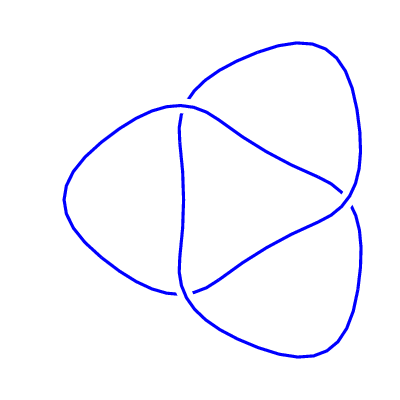
\includegraphics[width=\linewidth]{../data/3_1.png}
		\subcaption{$3_{1}$}
	\end{minipage}
	\begin{minipage}[b]{.18\linewidth}
		\centering
		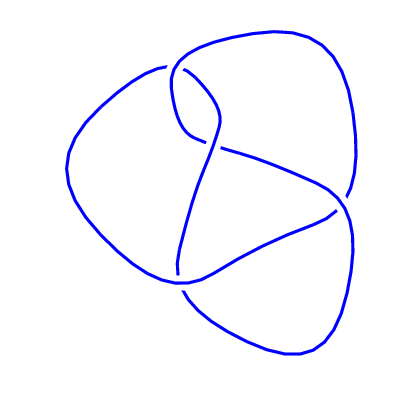
\includegraphics[width=\linewidth]{../data/4_1.png}
		\subcaption{$4_{1}$}
	\end{minipage}
	\begin{minipage}[b]{.18\linewidth}
		\centering
		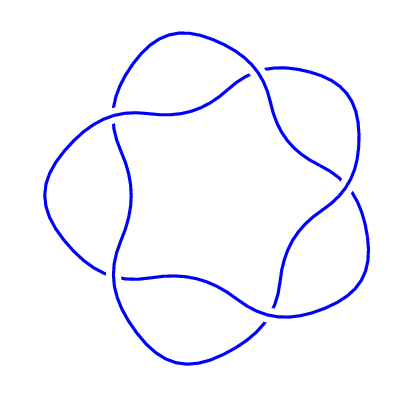
\includegraphics[width=\linewidth]{../data/5_1.png}
		\subcaption{$5_{1}$}
	\end{minipage}
	\begin{minipage}[b]{.18\linewidth}
		\centering
		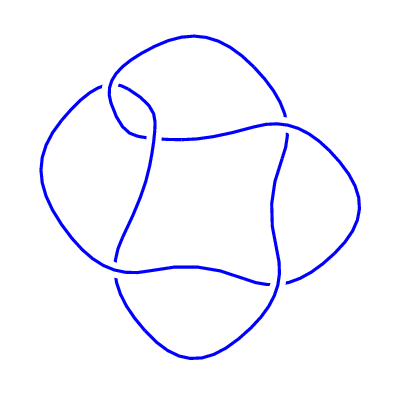
\includegraphics[width=\linewidth]{../data/5_2.png}
		\subcaption{$5_{2}$}
	\end{minipage}
	\begin{minipage}[b]{.18\linewidth}
		\centering
		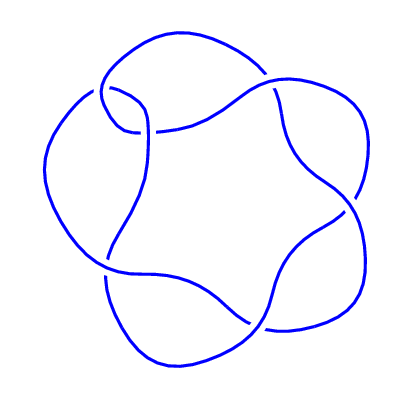
\includegraphics[width=\linewidth]{../data/6_1.png}
		\subcaption{$6_{1}$}
	\end{minipage}
\end{figure}
\begin{figure}[H]
	\begin{minipage}[b]{.18\linewidth}
		\centering
		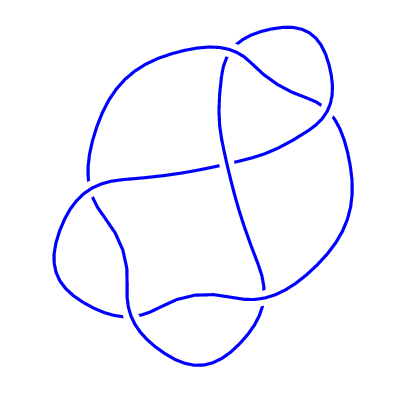
\includegraphics[width=\linewidth]{../data/6_2.png}
		\subcaption{$6_{2}$}
	\end{minipage}
	\begin{minipage}[b]{.18\linewidth}
		\centering
		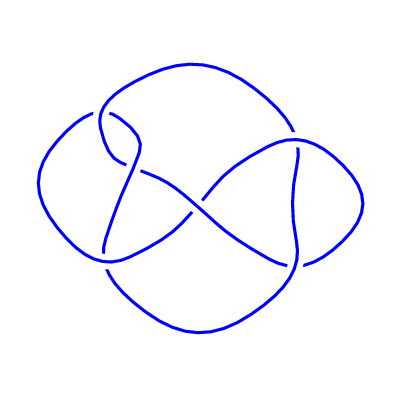
\includegraphics[width=\linewidth]{../data/6_3.png}
		\subcaption{$6_{3}$}
	\end{minipage}
	\begin{minipage}[b]{.18\linewidth}
		\centering
		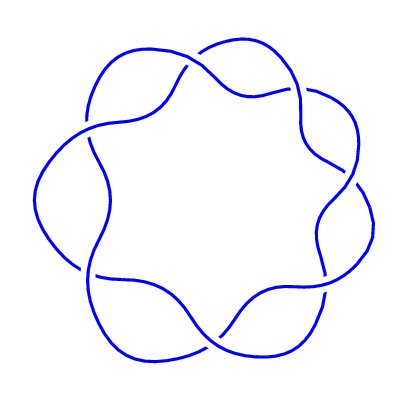
\includegraphics[width=\linewidth]{../data/7_1.png}
		\subcaption{$7_{1}$}
	\end{minipage}
	\begin{minipage}[b]{.18\linewidth}
		\centering
		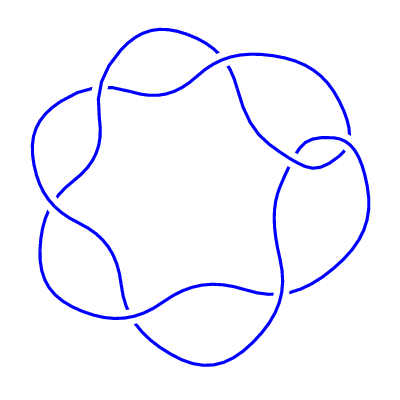
\includegraphics[width=\linewidth]{../data/7_2.png}
		\subcaption{$7_{2}$}
	\end{minipage}
	\begin{minipage}[b]{.18\linewidth}
		\centering
		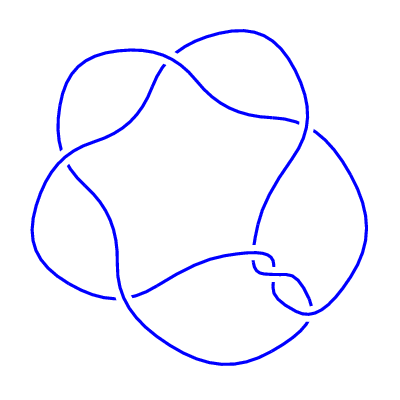
\includegraphics[width=\linewidth]{../data/7_3.png}
		\subcaption{$7_{3}$}
	\end{minipage}
\end{figure}
\begin{figure}[H]
	\begin{minipage}[b]{.18\linewidth}
		\centering
		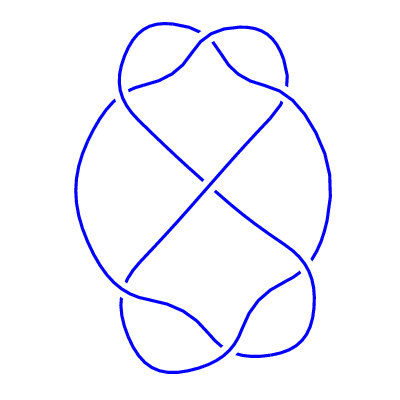
\includegraphics[width=\linewidth]{../data/7_4.png}
		\subcaption{$7_{4}$}
	\end{minipage}
	\begin{minipage}[b]{.18\linewidth}
		\centering
		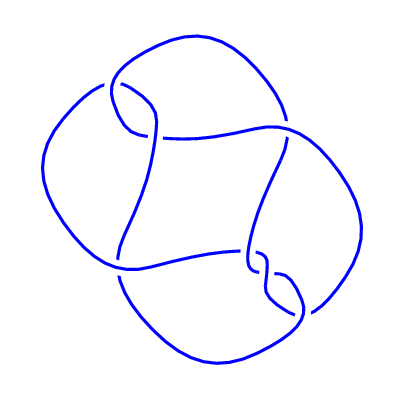
\includegraphics[width=\linewidth]{../data/7_5.png}
		\subcaption{$7_{5}$}
	\end{minipage}
	\begin{minipage}[b]{.18\linewidth}
		\centering
		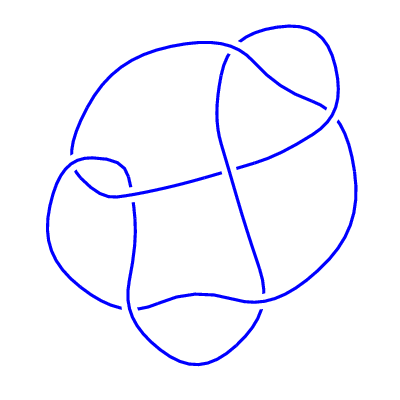
\includegraphics[width=\linewidth]{../data/7_6.png}
		\subcaption{$7_{6}$}
	\end{minipage}
	\begin{minipage}[b]{.18\linewidth}
		\centering
		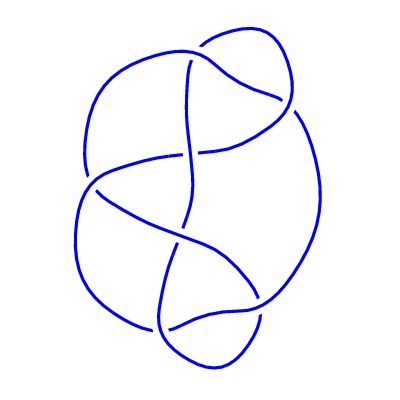
\includegraphics[width=\linewidth]{../data/7_7.png}
		\subcaption{$7_{7}$}
	\end{minipage}
	\begin{minipage}[b]{.18\linewidth}
		\centering
		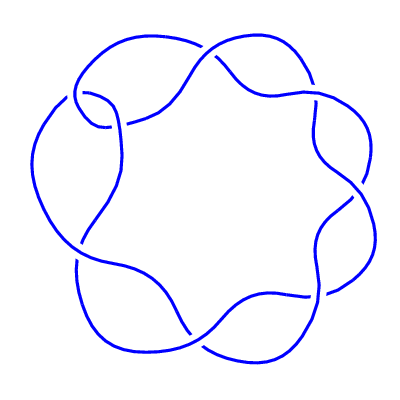
\includegraphics[width=\linewidth]{../data/8_1.png}
		\subcaption{$8_{1}$}
	\end{minipage}
\end{figure}
\begin{figure}[H]
	\begin{minipage}[b]{.18\linewidth}
		\centering
		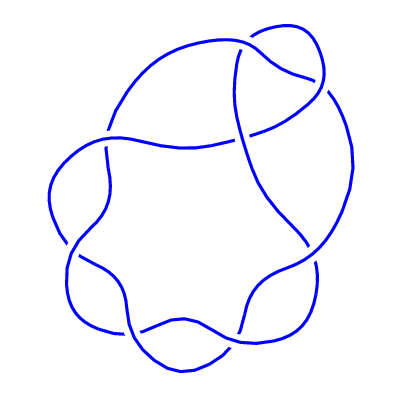
\includegraphics[width=\linewidth]{../data/8_2.png}
		\subcaption{$8_{2}$}
	\end{minipage}
	\begin{minipage}[b]{.18\linewidth}
		\centering
		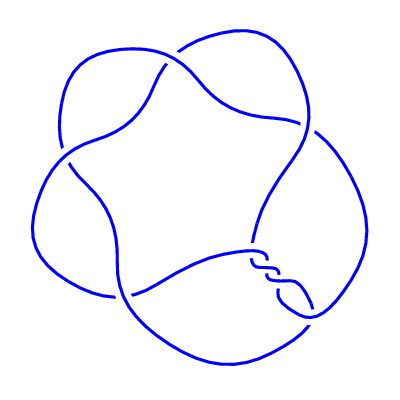
\includegraphics[width=\linewidth]{../data/8_3.png}
		\subcaption{$8_{3}$}
	\end{minipage}
	\begin{minipage}[b]{.18\linewidth}
		\centering
		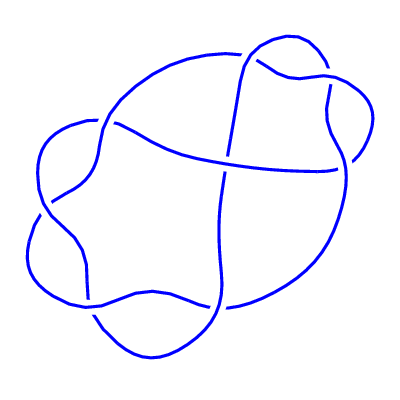
\includegraphics[width=\linewidth]{../data/8_4.png}
		\subcaption{$8_{4}$}
	\end{minipage}
	\begin{minipage}[b]{.18\linewidth}
		\centering
		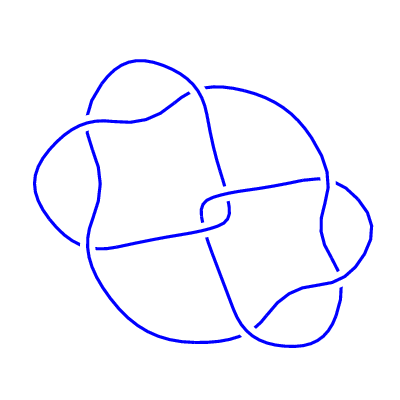
\includegraphics[width=\linewidth]{../data/8_5.png}
		\subcaption{$8_{5}$}
	\end{minipage}
	\begin{minipage}[b]{.18\linewidth}
		\centering
		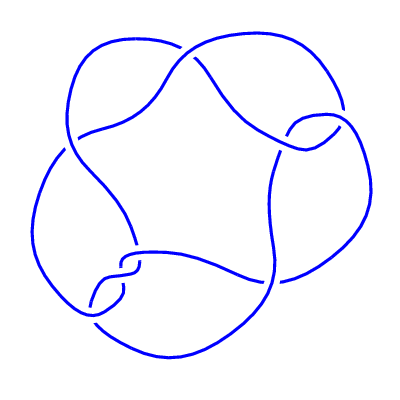
\includegraphics[width=\linewidth]{../data/8_6.png}
		\subcaption{$8_{6}$}
	\end{minipage}
\end{figure}
\begin{figure}[H]
	\begin{minipage}[b]{.18\linewidth}
		\centering
		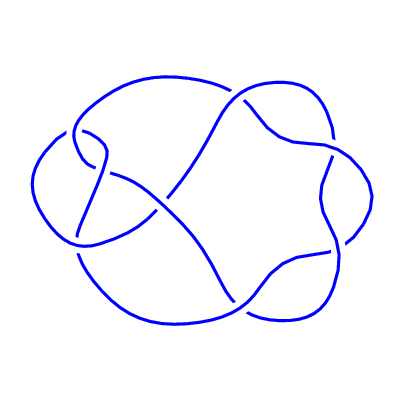
\includegraphics[width=\linewidth]{../data/8_7.png}
		\subcaption{$8_{7}$}
	\end{minipage}
	\begin{minipage}[b]{.18\linewidth}
		\centering
		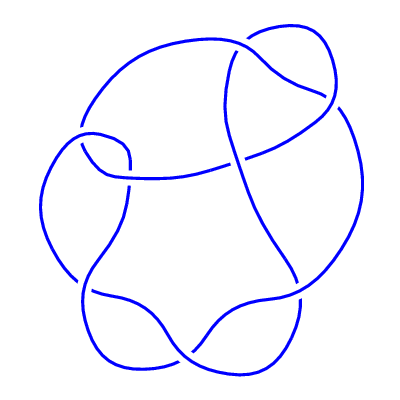
\includegraphics[width=\linewidth]{../data/8_8.png}
		\subcaption{$8_{8}$}
	\end{minipage}
	\begin{minipage}[b]{.18\linewidth}
		\centering
		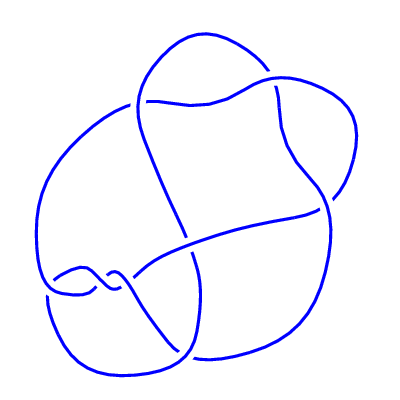
\includegraphics[width=\linewidth]{../data/8_9.png}
		\subcaption{$8_{9}$}
	\end{minipage}
	\begin{minipage}[b]{.18\linewidth}
		\centering
		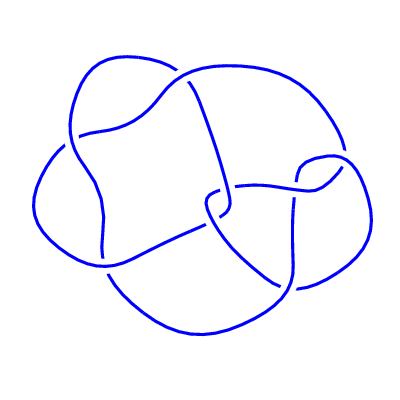
\includegraphics[width=\linewidth]{../data/8_10.png}
		\subcaption{$8_{10}$}
	\end{minipage}
	\begin{minipage}[b]{.18\linewidth}
		\centering
		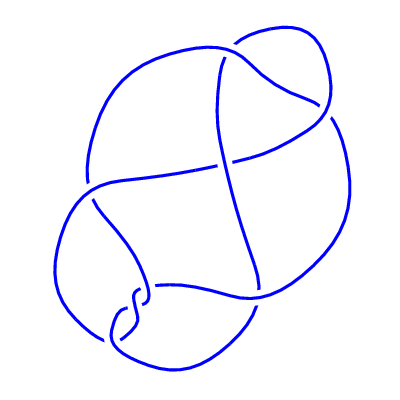
\includegraphics[width=\linewidth]{../data/8_11.png}
		\subcaption{$8_{11}$}
	\end{minipage}
\end{figure}
\begin{figure}[H]
	\begin{minipage}[b]{.18\linewidth}
		\centering
		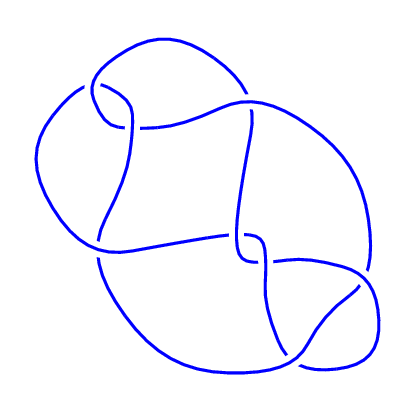
\includegraphics[width=\linewidth]{../data/8_12.png}
		\subcaption{$8_{12}$}
	\end{minipage}
	\begin{minipage}[b]{.18\linewidth}
		\centering
		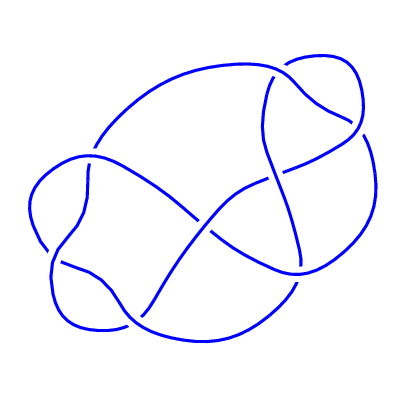
\includegraphics[width=\linewidth]{../data/8_13.png}
		\subcaption{$8_{13}$}
	\end{minipage}
	\begin{minipage}[b]{.18\linewidth}
		\centering
		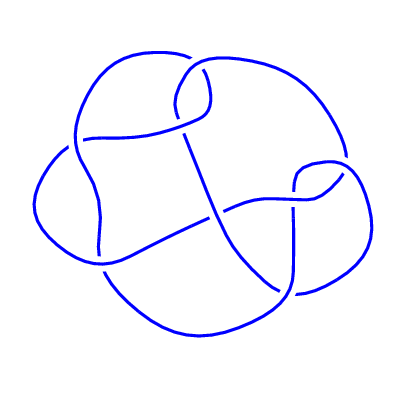
\includegraphics[width=\linewidth]{../data/8_14.png}
		\subcaption{$8_{14}$}
	\end{minipage}
	\begin{minipage}[b]{.18\linewidth}
		\centering
		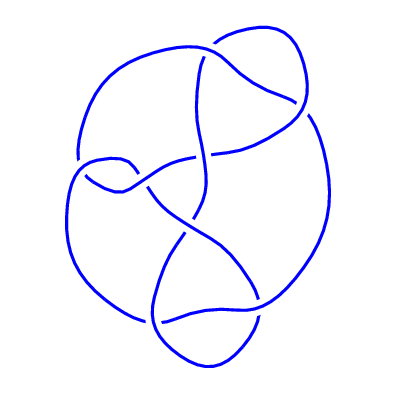
\includegraphics[width=\linewidth]{../data/8_15.png}
		\subcaption{$8_{15}$}
	\end{minipage}
	\begin{minipage}[b]{.18\linewidth}
		\centering
		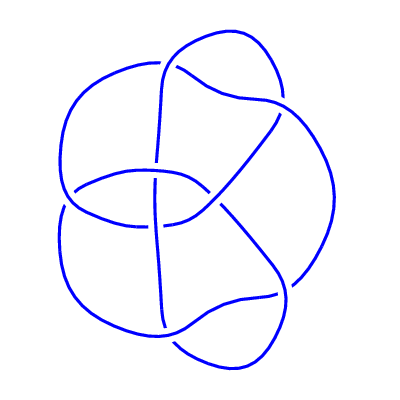
\includegraphics[width=\linewidth]{../data/8_16.png}
		\subcaption{$8_{16}$}
	\end{minipage}
\end{figure}
\begin{figure}[H]
	\begin{minipage}[b]{.18\linewidth}
		\centering
		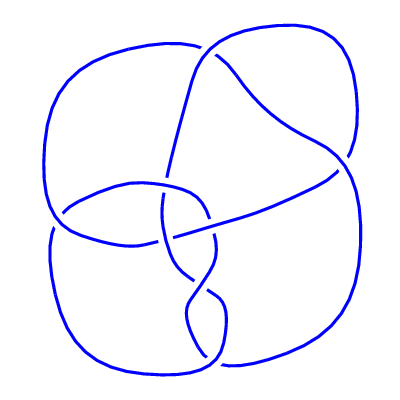
\includegraphics[width=\linewidth]{../data/8_17.png}
		\subcaption{$8_{17}$}
	\end{minipage}
	\begin{minipage}[b]{.18\linewidth}
		\centering
		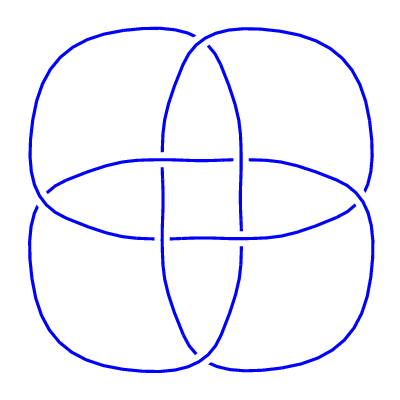
\includegraphics[width=\linewidth]{../data/8_18.png}
		\subcaption{$8_{18}$}
	\end{minipage}
	\begin{minipage}[b]{.18\linewidth}
		\centering
		\includegraphics[width=\linewidth]{../data/8_19.png}
		\subcaption{$8_{19}$}
	\end{minipage}
	\begin{minipage}[b]{.18\linewidth}
		\centering
		\includegraphics[width=\linewidth]{../data/8_20.png}
		\subcaption{$8_{20}$}
	\end{minipage}
	\begin{minipage}[b]{.18\linewidth}
		\centering
		\includegraphics[width=\linewidth]{../data/8_21.png}
		\subcaption{$8_{21}$}
	\end{minipage}
\end{figure}
\begin{figure}[H]
	\begin{minipage}[b]{.18\linewidth}
		\centering
		\includegraphics[width=\linewidth]{../data/9_1.png}
		\subcaption{$9_{1}$}
	\end{minipage}
	\begin{minipage}[b]{.18\linewidth}
		\centering
		\includegraphics[width=\linewidth]{../data/9_2.png}
		\subcaption{$9_{2}$}
	\end{minipage}
	\begin{minipage}[b]{.18\linewidth}
		\centering
		\includegraphics[width=\linewidth]{../data/9_3.png}
		\subcaption{$9_{3}$}
	\end{minipage}
	\begin{minipage}[b]{.18\linewidth}
		\centering
		\includegraphics[width=\linewidth]{../data/9_4.png}
		\subcaption{$9_{4}$}
	\end{minipage}
	\begin{minipage}[b]{.18\linewidth}
		\centering
		\includegraphics[width=\linewidth]{../data/9_5.png}
		\subcaption{$9_{5}$}
	\end{minipage}
\end{figure}
\begin{figure}[H]
	\begin{minipage}[b]{.18\linewidth}
		\centering
		\includegraphics[width=\linewidth]{../data/9_6.png}
		\subcaption{$9_{6}$}
	\end{minipage}
	\begin{minipage}[b]{.18\linewidth}
		\centering
		\includegraphics[width=\linewidth]{../data/9_7.png}
		\subcaption{$9_{7}$}
	\end{minipage}
	\begin{minipage}[b]{.18\linewidth}
		\centering
		\includegraphics[width=\linewidth]{../data/9_8.png}
		\subcaption{$9_{8}$}
	\end{minipage}
	\begin{minipage}[b]{.18\linewidth}
		\centering
		\includegraphics[width=\linewidth]{../data/9_9.png}
		\subcaption{$9_{9}$}
	\end{minipage}
	\begin{minipage}[b]{.18\linewidth}
		\centering
		\includegraphics[width=\linewidth]{../data/9_10.png}
		\subcaption{$9_{10}$}
	\end{minipage}
\end{figure}
\begin{figure}[H]
	\begin{minipage}[b]{.18\linewidth}
		\centering
		\includegraphics[width=\linewidth]{../data/9_11.png}
		\subcaption{$9_{11}$}
	\end{minipage}
	\begin{minipage}[b]{.18\linewidth}
		\centering
		\includegraphics[width=\linewidth]{../data/9_12.png}
		\subcaption{$9_{12}$}
	\end{minipage}
	\begin{minipage}[b]{.18\linewidth}
		\centering
		\includegraphics[width=\linewidth]{../data/9_13.png}
		\subcaption{$9_{13}$}
	\end{minipage}
	\begin{minipage}[b]{.18\linewidth}
		\centering
		\includegraphics[width=\linewidth]{../data/9_14.png}
		\subcaption{$9_{14}$}
	\end{minipage}
	\begin{minipage}[b]{.18\linewidth}
		\centering
		\includegraphics[width=\linewidth]{../data/9_15.png}
		\subcaption{$9_{15}$}
	\end{minipage}
\end{figure}
\begin{figure}[H]
	\begin{minipage}[b]{.18\linewidth}
		\centering
		\includegraphics[width=\linewidth]{../data/9_16.png}
		\subcaption{$9_{16}$}
	\end{minipage}
	\begin{minipage}[b]{.18\linewidth}
		\centering
		\includegraphics[width=\linewidth]{../data/9_17.png}
		\subcaption{$9_{17}$}
	\end{minipage}
	\begin{minipage}[b]{.18\linewidth}
		\centering
		\includegraphics[width=\linewidth]{../data/9_18.png}
		\subcaption{$9_{18}$}
	\end{minipage}
	\begin{minipage}[b]{.18\linewidth}
		\centering
		\includegraphics[width=\linewidth]{../data/9_19.png}
		\subcaption{$9_{19}$}
	\end{minipage}
	\begin{minipage}[b]{.18\linewidth}
		\centering
		\includegraphics[width=\linewidth]{../data/9_20.png}
		\subcaption{$9_{20}$}
	\end{minipage}
\end{figure}
\begin{figure}[H]
	\begin{minipage}[b]{.18\linewidth}
		\centering
		\includegraphics[width=\linewidth]{../data/9_21.png}
		\subcaption{$9_{21}$}
	\end{minipage}
	\begin{minipage}[b]{.18\linewidth}
		\centering
		\includegraphics[width=\linewidth]{../data/9_22.png}
		\subcaption{$9_{22}$}
	\end{minipage}
	\begin{minipage}[b]{.18\linewidth}
		\centering
		\includegraphics[width=\linewidth]{../data/9_23.png}
		\subcaption{$9_{23}$}
	\end{minipage}
	\begin{minipage}[b]{.18\linewidth}
		\centering
		\includegraphics[width=\linewidth]{../data/9_24.png}
		\subcaption{$9_{24}$}
	\end{minipage}
	\begin{minipage}[b]{.18\linewidth}
		\centering
		\includegraphics[width=\linewidth]{../data/9_25.png}
		\subcaption{$9_{25}$}
	\end{minipage}
\end{figure}
\begin{figure}[H]
	\begin{minipage}[b]{.18\linewidth}
		\centering
		\includegraphics[width=\linewidth]{../data/9_26.png}
		\subcaption{$9_{26}$}
	\end{minipage}
	\begin{minipage}[b]{.18\linewidth}
		\centering
		\includegraphics[width=\linewidth]{../data/9_27.png}
		\subcaption{$9_{27}$}
	\end{minipage}
	\begin{minipage}[b]{.18\linewidth}
		\centering
		\includegraphics[width=\linewidth]{../data/9_28.png}
		\subcaption{$9_{28}$}
	\end{minipage}
	\begin{minipage}[b]{.18\linewidth}
		\centering
		\includegraphics[width=\linewidth]{../data/9_29.png}
		\subcaption{$9_{29}$}
	\end{minipage}
	\begin{minipage}[b]{.18\linewidth}
		\centering
		\includegraphics[width=\linewidth]{../data/9_30.png}
		\subcaption{$9_{30}$}
	\end{minipage}
\end{figure}
\begin{figure}[H]
	\begin{minipage}[b]{.18\linewidth}
		\centering
		\includegraphics[width=\linewidth]{../data/9_31.png}
		\subcaption{$9_{31}$}
	\end{minipage}
	\begin{minipage}[b]{.18\linewidth}
		\centering
		\includegraphics[width=\linewidth]{../data/9_32.png}
		\subcaption{$9_{32}$}
	\end{minipage}
	\begin{minipage}[b]{.18\linewidth}
		\centering
		\includegraphics[width=\linewidth]{../data/9_33.png}
		\subcaption{$9_{33}$}
	\end{minipage}
	\begin{minipage}[b]{.18\linewidth}
		\centering
		\includegraphics[width=\linewidth]{../data/9_34.png}
		\subcaption{$9_{34}$}
	\end{minipage}
	\begin{minipage}[b]{.18\linewidth}
		\centering
		\includegraphics[width=\linewidth]{../data/9_35.png}
		\subcaption{$9_{35}$}
	\end{minipage}
\end{figure}
\begin{figure}[H]
	\begin{minipage}[b]{.18\linewidth}
		\centering
		\includegraphics[width=\linewidth]{../data/9_36.png}
		\subcaption{$9_{36}$}
	\end{minipage}
	\begin{minipage}[b]{.18\linewidth}
		\centering
		\includegraphics[width=\linewidth]{../data/9_37.png}
		\subcaption{$9_{37}$}
	\end{minipage}
	\begin{minipage}[b]{.18\linewidth}
		\centering
		\includegraphics[width=\linewidth]{../data/9_38.png}
		\subcaption{$9_{38}$}
	\end{minipage}
	\begin{minipage}[b]{.18\linewidth}
		\centering
		\includegraphics[width=\linewidth]{../data/9_39.png}
		\subcaption{$9_{39}$}
	\end{minipage}
	\begin{minipage}[b]{.18\linewidth}
		\centering
		\includegraphics[width=\linewidth]{../data/9_40.png}
		\subcaption{$9_{40}$}
	\end{minipage}
\end{figure}
\begin{figure}[H]
	\begin{minipage}[b]{.18\linewidth}
		\centering
		\includegraphics[width=\linewidth]{../data/9_41.png}
		\subcaption{$9_{41}$}
	\end{minipage}
	\begin{minipage}[b]{.18\linewidth}
		\centering
		\includegraphics[width=\linewidth]{../data/9_42.png}
		\subcaption{$9_{42}$}
	\end{minipage}
	\begin{minipage}[b]{.18\linewidth}
		\centering
		\includegraphics[width=\linewidth]{../data/9_43.png}
		\subcaption{$9_{43}$}
	\end{minipage}
	\begin{minipage}[b]{.18\linewidth}
		\centering
		\includegraphics[width=\linewidth]{../data/9_44.png}
		\subcaption{$9_{44}$}
	\end{minipage}
	\begin{minipage}[b]{.18\linewidth}
		\centering
		\includegraphics[width=\linewidth]{../data/9_45.png}
		\subcaption{$9_{45}$}
	\end{minipage}
\end{figure}
\begin{figure}[H]
	\begin{minipage}[b]{.18\linewidth}
		\centering
		\includegraphics[width=\linewidth]{../data/9_46.png}
		\subcaption{$9_{46}$}
	\end{minipage}
	\begin{minipage}[b]{.18\linewidth}
		\centering
		\includegraphics[width=\linewidth]{../data/9_47.png}
		\subcaption{$9_{47}$}
	\end{minipage}
	\begin{minipage}[b]{.18\linewidth}
		\centering
		\includegraphics[width=\linewidth]{../data/9_48.png}
		\subcaption{$9_{48}$}
	\end{minipage}
	\begin{minipage}[b]{.18\linewidth}
		\centering
		\includegraphics[width=\linewidth]{../data/9_49.png}
		\subcaption{$9_{49}$}
	\end{minipage}
	\begin{minipage}[b]{.18\linewidth}
		\centering
		\includegraphics[width=\linewidth]{../data/10_1.png}
		\subcaption{$10_{1}$}
	\end{minipage}
\end{figure}
\begin{figure}[H]
	\begin{minipage}[b]{.18\linewidth}
		\centering
		\includegraphics[width=\linewidth]{../data/10_2.png}
		\subcaption{$10_{2}$}
	\end{minipage}
	\begin{minipage}[b]{.18\linewidth}
		\centering
		\includegraphics[width=\linewidth]{../data/10_3.png}
		\subcaption{$10_{3}$}
	\end{minipage}
	\begin{minipage}[b]{.18\linewidth}
		\centering
		\includegraphics[width=\linewidth]{../data/10_4.png}
		\subcaption{$10_{4}$}
	\end{minipage}
	\begin{minipage}[b]{.18\linewidth}
		\centering
		\includegraphics[width=\linewidth]{../data/10_5.png}
		\subcaption{$10_{5}$}
	\end{minipage}
	\begin{minipage}[b]{.18\linewidth}
		\centering
		\includegraphics[width=\linewidth]{../data/10_6.png}
		\subcaption{$10_{6}$}
	\end{minipage}
\end{figure}
\begin{figure}[H]
	\begin{minipage}[b]{.18\linewidth}
		\centering
		\includegraphics[width=\linewidth]{../data/10_7.png}
		\subcaption{$10_{7}$}
	\end{minipage}
	\begin{minipage}[b]{.18\linewidth}
		\centering
		\includegraphics[width=\linewidth]{../data/10_8.png}
		\subcaption{$10_{8}$}
	\end{minipage}
	\begin{minipage}[b]{.18\linewidth}
		\centering
		\includegraphics[width=\linewidth]{../data/10_9.png}
		\subcaption{$10_{9}$}
	\end{minipage}
	\begin{minipage}[b]{.18\linewidth}
		\centering
		\includegraphics[width=\linewidth]{../data/10_10.png}
		\subcaption{$10_{10}$}
	\end{minipage}
	\begin{minipage}[b]{.18\linewidth}
		\centering
		\includegraphics[width=\linewidth]{../data/10_11.png}
		\subcaption{$10_{11}$}
	\end{minipage}
\end{figure}
\begin{figure}[H]
	\begin{minipage}[b]{.18\linewidth}
		\centering
		\includegraphics[width=\linewidth]{../data/10_12.png}
		\subcaption{$10_{12}$}
	\end{minipage}
	\begin{minipage}[b]{.18\linewidth}
		\centering
		\includegraphics[width=\linewidth]{../data/10_13.png}
		\subcaption{$10_{13}$}
	\end{minipage}
	\begin{minipage}[b]{.18\linewidth}
		\centering
		\includegraphics[width=\linewidth]{../data/10_14.png}
		\subcaption{$10_{14}$}
	\end{minipage}
	\begin{minipage}[b]{.18\linewidth}
		\centering
		\includegraphics[width=\linewidth]{../data/10_15.png}
		\subcaption{$10_{15}$}
	\end{minipage}
	\begin{minipage}[b]{.18\linewidth}
		\centering
		\includegraphics[width=\linewidth]{../data/10_16.png}
		\subcaption{$10_{16}$}
	\end{minipage}
\end{figure}
\begin{figure}[H]
	\begin{minipage}[b]{.18\linewidth}
		\centering
		\includegraphics[width=\linewidth]{../data/10_17.png}
		\subcaption{$10_{17}$}
	\end{minipage}
	\begin{minipage}[b]{.18\linewidth}
		\centering
		\includegraphics[width=\linewidth]{../data/10_18.png}
		\subcaption{$10_{18}$}
	\end{minipage}
	\begin{minipage}[b]{.18\linewidth}
		\centering
		\includegraphics[width=\linewidth]{../data/10_19.png}
		\subcaption{$10_{19}$}
	\end{minipage}
	\begin{minipage}[b]{.18\linewidth}
		\centering
		\includegraphics[width=\linewidth]{../data/10_20.png}
		\subcaption{$10_{20}$}
	\end{minipage}
	\begin{minipage}[b]{.18\linewidth}
		\centering
		\includegraphics[width=\linewidth]{../data/10_21.png}
		\subcaption{$10_{21}$}
	\end{minipage}
\end{figure}
\begin{figure}[H]
	\begin{minipage}[b]{.18\linewidth}
		\centering
		\includegraphics[width=\linewidth]{../data/10_22.png}
		\subcaption{$10_{22}$}
	\end{minipage}
	\begin{minipage}[b]{.18\linewidth}
		\centering
		\includegraphics[width=\linewidth]{../data/10_23.png}
		\subcaption{$10_{23}$}
	\end{minipage}
	\begin{minipage}[b]{.18\linewidth}
		\centering
		\includegraphics[width=\linewidth]{../data/10_24.png}
		\subcaption{$10_{24}$}
	\end{minipage}
	\begin{minipage}[b]{.18\linewidth}
		\centering
		\includegraphics[width=\linewidth]{../data/10_25.png}
		\subcaption{$10_{25}$}
	\end{minipage}
	\begin{minipage}[b]{.18\linewidth}
		\centering
		\includegraphics[width=\linewidth]{../data/10_26.png}
		\subcaption{$10_{26}$}
	\end{minipage}
\end{figure}
\begin{figure}[H]
	\begin{minipage}[b]{.18\linewidth}
		\centering
		\includegraphics[width=\linewidth]{../data/10_27.png}
		\subcaption{$10_{27}$}
	\end{minipage}
	\begin{minipage}[b]{.18\linewidth}
		\centering
		\includegraphics[width=\linewidth]{../data/10_28.png}
		\subcaption{$10_{28}$}
	\end{minipage}
	\begin{minipage}[b]{.18\linewidth}
		\centering
		\includegraphics[width=\linewidth]{../data/10_29.png}
		\subcaption{$10_{29}$}
	\end{minipage}
	\begin{minipage}[b]{.18\linewidth}
		\centering
		\includegraphics[width=\linewidth]{../data/10_30.png}
		\subcaption{$10_{30}$}
	\end{minipage}
	\begin{minipage}[b]{.18\linewidth}
		\centering
		\includegraphics[width=\linewidth]{../data/10_31.png}
		\subcaption{$10_{31}$}
	\end{minipage}
\end{figure}
\begin{figure}[H]
	\begin{minipage}[b]{.18\linewidth}
		\centering
		\includegraphics[width=\linewidth]{../data/10_32.png}
		\subcaption{$10_{32}$}
	\end{minipage}
	\begin{minipage}[b]{.18\linewidth}
		\centering
		\includegraphics[width=\linewidth]{../data/10_33.png}
		\subcaption{$10_{33}$}
	\end{minipage}
	\begin{minipage}[b]{.18\linewidth}
		\centering
		\includegraphics[width=\linewidth]{../data/10_34.png}
		\subcaption{$10_{34}$}
	\end{minipage}
	\begin{minipage}[b]{.18\linewidth}
		\centering
		\includegraphics[width=\linewidth]{../data/10_35.png}
		\subcaption{$10_{35}$}
	\end{minipage}
	\begin{minipage}[b]{.18\linewidth}
		\centering
		\includegraphics[width=\linewidth]{../data/10_36.png}
		\subcaption{$10_{36}$}
	\end{minipage}
\end{figure}
\begin{figure}[H]
	\begin{minipage}[b]{.18\linewidth}
		\centering
		\includegraphics[width=\linewidth]{../data/10_37.png}
		\subcaption{$10_{37}$}
	\end{minipage}
	\begin{minipage}[b]{.18\linewidth}
		\centering
		\includegraphics[width=\linewidth]{../data/10_38.png}
		\subcaption{$10_{38}$}
	\end{minipage}
	\begin{minipage}[b]{.18\linewidth}
		\centering
		\includegraphics[width=\linewidth]{../data/10_39.png}
		\subcaption{$10_{39}$}
	\end{minipage}
	\begin{minipage}[b]{.18\linewidth}
		\centering
		\includegraphics[width=\linewidth]{../data/10_40.png}
		\subcaption{$10_{40}$}
	\end{minipage}
	\begin{minipage}[b]{.18\linewidth}
		\centering
		\includegraphics[width=\linewidth]{../data/10_41.png}
		\subcaption{$10_{41}$}
	\end{minipage}
\end{figure}
\begin{figure}[H]
	\begin{minipage}[b]{.18\linewidth}
		\centering
		\includegraphics[width=\linewidth]{../data/10_42.png}
		\subcaption{$10_{42}$}
	\end{minipage}
	\begin{minipage}[b]{.18\linewidth}
		\centering
		\includegraphics[width=\linewidth]{../data/10_43.png}
		\subcaption{$10_{43}$}
	\end{minipage}
	\begin{minipage}[b]{.18\linewidth}
		\centering
		\includegraphics[width=\linewidth]{../data/10_44.png}
		\subcaption{$10_{44}$}
	\end{minipage}
	\begin{minipage}[b]{.18\linewidth}
		\centering
		\includegraphics[width=\linewidth]{../data/10_45.png}
		\subcaption{$10_{45}$}
	\end{minipage}
	\begin{minipage}[b]{.18\linewidth}
		\centering
		\includegraphics[width=\linewidth]{../data/10_46.png}
		\subcaption{$10_{46}$}
	\end{minipage}
\end{figure}
\begin{figure}[H]
	\begin{minipage}[b]{.18\linewidth}
		\centering
		\includegraphics[width=\linewidth]{../data/10_47.png}
		\subcaption{$10_{47}$}
	\end{minipage}
	\begin{minipage}[b]{.18\linewidth}
		\centering
		\includegraphics[width=\linewidth]{../data/10_48.png}
		\subcaption{$10_{48}$}
	\end{minipage}
	\begin{minipage}[b]{.18\linewidth}
		\centering
		\includegraphics[width=\linewidth]{../data/10_49.png}
		\subcaption{$10_{49}$}
	\end{minipage}
	\begin{minipage}[b]{.18\linewidth}
		\centering
		\includegraphics[width=\linewidth]{../data/10_50.png}
		\subcaption{$10_{50}$}
	\end{minipage}
	\begin{minipage}[b]{.18\linewidth}
		\centering
		\includegraphics[width=\linewidth]{../data/10_51.png}
		\subcaption{$10_{51}$}
	\end{minipage}
\end{figure}
\begin{figure}[H]
	\begin{minipage}[b]{.18\linewidth}
		\centering
		\includegraphics[width=\linewidth]{../data/10_52.png}
		\subcaption{$10_{52}$}
	\end{minipage}
	\begin{minipage}[b]{.18\linewidth}
		\centering
		\includegraphics[width=\linewidth]{../data/10_53.png}
		\subcaption{$10_{53}$}
	\end{minipage}
	\begin{minipage}[b]{.18\linewidth}
		\centering
		\includegraphics[width=\linewidth]{../data/10_54.png}
		\subcaption{$10_{54}$}
	\end{minipage}
	\begin{minipage}[b]{.18\linewidth}
		\centering
		\includegraphics[width=\linewidth]{../data/10_55.png}
		\subcaption{$10_{55}$}
	\end{minipage}
	\begin{minipage}[b]{.18\linewidth}
		\centering
		\includegraphics[width=\linewidth]{../data/10_56.png}
		\subcaption{$10_{56}$}
	\end{minipage}
\end{figure}
\begin{figure}[H]
	\begin{minipage}[b]{.18\linewidth}
		\centering
		\includegraphics[width=\linewidth]{../data/10_57.png}
		\subcaption{$10_{57}$}
	\end{minipage}
	\begin{minipage}[b]{.18\linewidth}
		\centering
		\includegraphics[width=\linewidth]{../data/10_58.png}
		\subcaption{$10_{58}$}
	\end{minipage}
	\begin{minipage}[b]{.18\linewidth}
		\centering
		\includegraphics[width=\linewidth]{../data/10_59.png}
		\subcaption{$10_{59}$}
	\end{minipage}
	\begin{minipage}[b]{.18\linewidth}
		\centering
		\includegraphics[width=\linewidth]{../data/10_60.png}
		\subcaption{$10_{60}$}
	\end{minipage}
	\begin{minipage}[b]{.18\linewidth}
		\centering
		\includegraphics[width=\linewidth]{../data/10_61.png}
		\subcaption{$10_{61}$}
	\end{minipage}
\end{figure}
\begin{figure}[H]
	\begin{minipage}[b]{.18\linewidth}
		\centering
		\includegraphics[width=\linewidth]{../data/10_62.png}
		\subcaption{$10_{62}$}
	\end{minipage}
	\begin{minipage}[b]{.18\linewidth}
		\centering
		\includegraphics[width=\linewidth]{../data/10_63.png}
		\subcaption{$10_{63}$}
	\end{minipage}
	\begin{minipage}[b]{.18\linewidth}
		\centering
		\includegraphics[width=\linewidth]{../data/10_64.png}
		\subcaption{$10_{64}$}
	\end{minipage}
	\begin{minipage}[b]{.18\linewidth}
		\centering
		\includegraphics[width=\linewidth]{../data/10_65.png}
		\subcaption{$10_{65}$}
	\end{minipage}
	\begin{minipage}[b]{.18\linewidth}
		\centering
		\includegraphics[width=\linewidth]{../data/10_66.png}
		\subcaption{$10_{66}$}
	\end{minipage}
\end{figure}
\begin{figure}[H]
	\begin{minipage}[b]{.18\linewidth}
		\centering
		\includegraphics[width=\linewidth]{../data/10_67.png}
		\subcaption{$10_{67}$}
	\end{minipage}
	\begin{minipage}[b]{.18\linewidth}
		\centering
		\includegraphics[width=\linewidth]{../data/10_68.png}
		\subcaption{$10_{68}$}
	\end{minipage}
	\begin{minipage}[b]{.18\linewidth}
		\centering
		\includegraphics[width=\linewidth]{../data/10_69.png}
		\subcaption{$10_{69}$}
	\end{minipage}
	\begin{minipage}[b]{.18\linewidth}
		\centering
		\includegraphics[width=\linewidth]{../data/10_70.png}
		\subcaption{$10_{70}$}
	\end{minipage}
	\begin{minipage}[b]{.18\linewidth}
		\centering
		\includegraphics[width=\linewidth]{../data/10_71.png}
		\subcaption{$10_{71}$}
	\end{minipage}
\end{figure}
\begin{figure}[H]
	\begin{minipage}[b]{.18\linewidth}
		\centering
		\includegraphics[width=\linewidth]{../data/10_72.png}
		\subcaption{$10_{72}$}
	\end{minipage}
	\begin{minipage}[b]{.18\linewidth}
		\centering
		\includegraphics[width=\linewidth]{../data/10_73.png}
		\subcaption{$10_{73}$}
	\end{minipage}
	\begin{minipage}[b]{.18\linewidth}
		\centering
		\includegraphics[width=\linewidth]{../data/10_74.png}
		\subcaption{$10_{74}$}
	\end{minipage}
	\begin{minipage}[b]{.18\linewidth}
		\centering
		\includegraphics[width=\linewidth]{../data/10_75.png}
		\subcaption{$10_{75}$}
	\end{minipage}
	\begin{minipage}[b]{.18\linewidth}
		\centering
		\includegraphics[width=\linewidth]{../data/10_76.png}
		\subcaption{$10_{76}$}
	\end{minipage}
\end{figure}
\begin{figure}[H]
	\begin{minipage}[b]{.18\linewidth}
		\centering
		\includegraphics[width=\linewidth]{../data/10_77.png}
		\subcaption{$10_{77}$}
	\end{minipage}
	\begin{minipage}[b]{.18\linewidth}
		\centering
		\includegraphics[width=\linewidth]{../data/10_78.png}
		\subcaption{$10_{78}$}
	\end{minipage}
	\begin{minipage}[b]{.18\linewidth}
		\centering
		\includegraphics[width=\linewidth]{../data/10_79.png}
		\subcaption{$10_{79}$}
	\end{minipage}
	\begin{minipage}[b]{.18\linewidth}
		\centering
		\includegraphics[width=\linewidth]{../data/10_80.png}
		\subcaption{$10_{80}$}
	\end{minipage}
	\begin{minipage}[b]{.18\linewidth}
		\centering
		\includegraphics[width=\linewidth]{../data/10_81.png}
		\subcaption{$10_{81}$}
	\end{minipage}
\end{figure}
\begin{figure}[H]
	\begin{minipage}[b]{.18\linewidth}
		\centering
		\includegraphics[width=\linewidth]{../data/10_82.png}
		\subcaption{$10_{82}$}
	\end{minipage}
	\begin{minipage}[b]{.18\linewidth}
		\centering
		\includegraphics[width=\linewidth]{../data/10_83.png}
		\subcaption{$10_{83}$}
	\end{minipage}
	\begin{minipage}[b]{.18\linewidth}
		\centering
		\includegraphics[width=\linewidth]{../data/10_84.png}
		\subcaption{$10_{84}$}
	\end{minipage}
	\begin{minipage}[b]{.18\linewidth}
		\centering
		\includegraphics[width=\linewidth]{../data/10_85.png}
		\subcaption{$10_{85}$}
	\end{minipage}
	\begin{minipage}[b]{.18\linewidth}
		\centering
		\includegraphics[width=\linewidth]{../data/10_86.png}
		\subcaption{$10_{86}$}
	\end{minipage}
\end{figure}
\begin{figure}[H]
	\begin{minipage}[b]{.18\linewidth}
		\centering
		\includegraphics[width=\linewidth]{../data/10_87.png}
		\subcaption{$10_{87}$}
	\end{minipage}
	\begin{minipage}[b]{.18\linewidth}
		\centering
		\includegraphics[width=\linewidth]{../data/10_88.png}
		\subcaption{$10_{88}$}
	\end{minipage}
	\begin{minipage}[b]{.18\linewidth}
		\centering
		\includegraphics[width=\linewidth]{../data/10_89.png}
		\subcaption{$10_{89}$}
	\end{minipage}
	\begin{minipage}[b]{.18\linewidth}
		\centering
		\includegraphics[width=\linewidth]{../data/10_90.png}
		\subcaption{$10_{90}$}
	\end{minipage}
	\begin{minipage}[b]{.18\linewidth}
		\centering
		\includegraphics[width=\linewidth]{../data/10_91.png}
		\subcaption{$10_{91}$}
	\end{minipage}
\end{figure}
\begin{figure}[H]
	\begin{minipage}[b]{.18\linewidth}
		\centering
		\includegraphics[width=\linewidth]{../data/10_92.png}
		\subcaption{$10_{92}$}
	\end{minipage}
	\begin{minipage}[b]{.18\linewidth}
		\centering
		\includegraphics[width=\linewidth]{../data/10_93.png}
		\subcaption{$10_{93}$}
	\end{minipage}
	\begin{minipage}[b]{.18\linewidth}
		\centering
		\includegraphics[width=\linewidth]{../data/10_94.png}
		\subcaption{$10_{94}$}
	\end{minipage}
	\begin{minipage}[b]{.18\linewidth}
		\centering
		\includegraphics[width=\linewidth]{../data/10_95.png}
		\subcaption{$10_{95}$}
	\end{minipage}
	\begin{minipage}[b]{.18\linewidth}
		\centering
		\includegraphics[width=\linewidth]{../data/10_96.png}
		\subcaption{$10_{96}$}
	\end{minipage}
\end{figure}
\begin{figure}[H]
	\begin{minipage}[b]{.18\linewidth}
		\centering
		\includegraphics[width=\linewidth]{../data/10_97.png}
		\subcaption{$10_{97}$}
	\end{minipage}
	\begin{minipage}[b]{.18\linewidth}
		\centering
		\includegraphics[width=\linewidth]{../data/10_98.png}
		\subcaption{$10_{98}$}
	\end{minipage}
	\begin{minipage}[b]{.18\linewidth}
		\centering
		\includegraphics[width=\linewidth]{../data/10_99.png}
		\subcaption{$10_{99}$}
	\end{minipage}
	\begin{minipage}[b]{.18\linewidth}
		\centering
		\includegraphics[width=\linewidth]{../data/10_100.png}
		\subcaption{$10_{100}$}
	\end{minipage}
	\begin{minipage}[b]{.18\linewidth}
		\centering
		\includegraphics[width=\linewidth]{../data/10_101.png}
		\subcaption{$10_{101}$}
	\end{minipage}
\end{figure}
\begin{figure}[H]
	\begin{minipage}[b]{.18\linewidth}
		\centering
		\includegraphics[width=\linewidth]{../data/10_102.png}
		\subcaption{$10_{102}$}
	\end{minipage}
	\begin{minipage}[b]{.18\linewidth}
		\centering
		\includegraphics[width=\linewidth]{../data/10_103.png}
		\subcaption{$10_{103}$}
	\end{minipage}
	\begin{minipage}[b]{.18\linewidth}
		\centering
		\includegraphics[width=\linewidth]{../data/10_104.png}
		\subcaption{$10_{104}$}
	\end{minipage}
	\begin{minipage}[b]{.18\linewidth}
		\centering
		\includegraphics[width=\linewidth]{../data/10_105.png}
		\subcaption{$10_{105}$}
	\end{minipage}
	\begin{minipage}[b]{.18\linewidth}
		\centering
		\includegraphics[width=\linewidth]{../data/10_106.png}
		\subcaption{$10_{106}$}
	\end{minipage}
\end{figure}
\begin{figure}[H]
	\begin{minipage}[b]{.18\linewidth}
		\centering
		\includegraphics[width=\linewidth]{../data/10_107.png}
		\subcaption{$10_{107}$}
	\end{minipage}
	\begin{minipage}[b]{.18\linewidth}
		\centering
		\includegraphics[width=\linewidth]{../data/10_108.png}
		\subcaption{$10_{108}$}
	\end{minipage}
	\begin{minipage}[b]{.18\linewidth}
		\centering
		\includegraphics[width=\linewidth]{../data/10_109.png}
		\subcaption{$10_{109}$}
	\end{minipage}
	\begin{minipage}[b]{.18\linewidth}
		\centering
		\includegraphics[width=\linewidth]{../data/10_110.png}
		\subcaption{$10_{110}$}
	\end{minipage}
	\begin{minipage}[b]{.18\linewidth}
		\centering
		\includegraphics[width=\linewidth]{../data/10_111.png}
		\subcaption{$10_{111}$}
	\end{minipage}
\end{figure}
\begin{figure}[H]
	\begin{minipage}[b]{.18\linewidth}
		\centering
		\includegraphics[width=\linewidth]{../data/10_112.png}
		\subcaption{$10_{112}$}
	\end{minipage}
	\begin{minipage}[b]{.18\linewidth}
		\centering
		\includegraphics[width=\linewidth]{../data/10_113.png}
		\subcaption{$10_{113}$}
	\end{minipage}
	\begin{minipage}[b]{.18\linewidth}
		\centering
		\includegraphics[width=\linewidth]{../data/10_114.png}
		\subcaption{$10_{114}$}
	\end{minipage}
	\begin{minipage}[b]{.18\linewidth}
		\centering
		\includegraphics[width=\linewidth]{../data/10_115.png}
		\subcaption{$10_{115}$}
	\end{minipage}
	\begin{minipage}[b]{.18\linewidth}
		\centering
		\includegraphics[width=\linewidth]{../data/10_116.png}
		\subcaption{$10_{116}$}
	\end{minipage}
\end{figure}
\begin{figure}[H]
	\begin{minipage}[b]{.18\linewidth}
		\centering
		\includegraphics[width=\linewidth]{../data/10_117.png}
		\subcaption{$10_{117}$}
	\end{minipage}
	\begin{minipage}[b]{.18\linewidth}
		\centering
		\includegraphics[width=\linewidth]{../data/10_118.png}
		\subcaption{$10_{118}$}
	\end{minipage}
	\begin{minipage}[b]{.18\linewidth}
		\centering
		\includegraphics[width=\linewidth]{../data/10_119.png}
		\subcaption{$10_{119}$}
	\end{minipage}
	\begin{minipage}[b]{.18\linewidth}
		\centering
		\includegraphics[width=\linewidth]{../data/10_120.png}
		\subcaption{$10_{120}$}
	\end{minipage}
	\begin{minipage}[b]{.18\linewidth}
		\centering
		\includegraphics[width=\linewidth]{../data/10_121.png}
		\subcaption{$10_{121}$}
	\end{minipage}
\end{figure}
\begin{figure}[H]
	\begin{minipage}[b]{.18\linewidth}
		\centering
		\includegraphics[width=\linewidth]{../data/10_122.png}
		\subcaption{$10_{122}$}
	\end{minipage}
	\begin{minipage}[b]{.18\linewidth}
		\centering
		\includegraphics[width=\linewidth]{../data/10_123.png}
		\subcaption{$10_{123}$}
	\end{minipage}
	\begin{minipage}[b]{.18\linewidth}
		\centering
		\includegraphics[width=\linewidth]{../data/10_124.png}
		\subcaption{$10_{124}$}
	\end{minipage}
	\begin{minipage}[b]{.18\linewidth}
		\centering
		\includegraphics[width=\linewidth]{../data/10_125.png}
		\subcaption{$10_{125}$}
	\end{minipage}
	\begin{minipage}[b]{.18\linewidth}
		\centering
		\includegraphics[width=\linewidth]{../data/10_126.png}
		\subcaption{$10_{126}$}
	\end{minipage}
\end{figure}
\begin{figure}[H]
	\begin{minipage}[b]{.18\linewidth}
		\centering
		\includegraphics[width=\linewidth]{../data/10_127.png}
		\subcaption{$10_{127}$}
	\end{minipage}
	\begin{minipage}[b]{.18\linewidth}
		\centering
		\includegraphics[width=\linewidth]{../data/10_128.png}
		\subcaption{$10_{128}$}
	\end{minipage}
	\begin{minipage}[b]{.18\linewidth}
		\centering
		\includegraphics[width=\linewidth]{../data/10_129.png}
		\subcaption{$10_{129}$}
	\end{minipage}
	\begin{minipage}[b]{.18\linewidth}
		\centering
		\includegraphics[width=\linewidth]{../data/10_130.png}
		\subcaption{$10_{130}$}
	\end{minipage}
	\begin{minipage}[b]{.18\linewidth}
		\centering
		\includegraphics[width=\linewidth]{../data/10_131.png}
		\subcaption{$10_{131}$}
	\end{minipage}
\end{figure}
\begin{figure}[H]
	\begin{minipage}[b]{.18\linewidth}
		\centering
		\includegraphics[width=\linewidth]{../data/10_132.png}
		\subcaption{$10_{132}$}
	\end{minipage}
	\begin{minipage}[b]{.18\linewidth}
		\centering
		\includegraphics[width=\linewidth]{../data/10_133.png}
		\subcaption{$10_{133}$}
	\end{minipage}
	\begin{minipage}[b]{.18\linewidth}
		\centering
		\includegraphics[width=\linewidth]{../data/10_134.png}
		\subcaption{$10_{134}$}
	\end{minipage}
	\begin{minipage}[b]{.18\linewidth}
		\centering
		\includegraphics[width=\linewidth]{../data/10_135.png}
		\subcaption{$10_{135}$}
	\end{minipage}
	\begin{minipage}[b]{.18\linewidth}
		\centering
		\includegraphics[width=\linewidth]{../data/10_136.png}
		\subcaption{$10_{136}$}
	\end{minipage}
\end{figure}
\begin{figure}[H]
	\begin{minipage}[b]{.18\linewidth}
		\centering
		\includegraphics[width=\linewidth]{../data/10_137.png}
		\subcaption{$10_{137}$}
	\end{minipage}
	\begin{minipage}[b]{.18\linewidth}
		\centering
		\includegraphics[width=\linewidth]{../data/10_138.png}
		\subcaption{$10_{138}$}
	\end{minipage}
	\begin{minipage}[b]{.18\linewidth}
		\centering
		\includegraphics[width=\linewidth]{../data/10_139.png}
		\subcaption{$10_{139}$}
	\end{minipage}
	\begin{minipage}[b]{.18\linewidth}
		\centering
		\includegraphics[width=\linewidth]{../data/10_140.png}
		\subcaption{$10_{140}$}
	\end{minipage}
	\begin{minipage}[b]{.18\linewidth}
		\centering
		\includegraphics[width=\linewidth]{../data/10_141.png}
		\subcaption{$10_{141}$}
	\end{minipage}
\end{figure}
\begin{figure}[H]
	\begin{minipage}[b]{.18\linewidth}
		\centering
		\includegraphics[width=\linewidth]{../data/10_142.png}
		\subcaption{$10_{142}$}
	\end{minipage}
	\begin{minipage}[b]{.18\linewidth}
		\centering
		\includegraphics[width=\linewidth]{../data/10_143.png}
		\subcaption{$10_{143}$}
	\end{minipage}
	\begin{minipage}[b]{.18\linewidth}
		\centering
		\includegraphics[width=\linewidth]{../data/10_144.png}
		\subcaption{$10_{144}$}
	\end{minipage}
	\begin{minipage}[b]{.18\linewidth}
		\centering
		\includegraphics[width=\linewidth]{../data/10_145.png}
		\subcaption{$10_{145}$}
	\end{minipage}
	\begin{minipage}[b]{.18\linewidth}
		\centering
		\includegraphics[width=\linewidth]{../data/10_146.png}
		\subcaption{$10_{146}$}
	\end{minipage}
\end{figure}
\begin{figure}[H]
	\begin{minipage}[b]{.18\linewidth}
		\centering
		\includegraphics[width=\linewidth]{../data/10_147.png}
		\subcaption{$10_{147}$}
	\end{minipage}
	\begin{minipage}[b]{.18\linewidth}
		\centering
		\includegraphics[width=\linewidth]{../data/10_148.png}
		\subcaption{$10_{148}$}
	\end{minipage}
	\begin{minipage}[b]{.18\linewidth}
		\centering
		\includegraphics[width=\linewidth]{../data/10_149.png}
		\subcaption{$10_{149}$}
	\end{minipage}
	\begin{minipage}[b]{.18\linewidth}
		\centering
		\includegraphics[width=\linewidth]{../data/10_150.png}
		\subcaption{$10_{150}$}
	\end{minipage}
	\begin{minipage}[b]{.18\linewidth}
		\centering
		\includegraphics[width=\linewidth]{../data/10_151.png}
		\subcaption{$10_{151}$}
	\end{minipage}
\end{figure}
\begin{figure}[H]
	\begin{minipage}[b]{.18\linewidth}
		\centering
		\includegraphics[width=\linewidth]{../data/10_152.png}
		\subcaption{$10_{152}$}
	\end{minipage}
	\begin{minipage}[b]{.18\linewidth}
		\centering
		\includegraphics[width=\linewidth]{../data/10_153.png}
		\subcaption{$10_{153}$}
	\end{minipage}
	\begin{minipage}[b]{.18\linewidth}
		\centering
		\includegraphics[width=\linewidth]{../data/10_154.png}
		\subcaption{$10_{154}$}
	\end{minipage}
	\begin{minipage}[b]{.18\linewidth}
		\centering
		\includegraphics[width=\linewidth]{../data/10_155.png}
		\subcaption{$10_{155}$}
	\end{minipage}
	\begin{minipage}[b]{.18\linewidth}
		\centering
		\includegraphics[width=\linewidth]{../data/10_156.png}
		\subcaption{$10_{156}$}
	\end{minipage}
\end{figure}
\begin{figure}[H]
	\begin{minipage}[b]{.18\linewidth}
		\centering
		\includegraphics[width=\linewidth]{../data/10_157.png}
		\subcaption{$10_{157}$}
	\end{minipage}
	\begin{minipage}[b]{.18\linewidth}
		\centering
		\includegraphics[width=\linewidth]{../data/10_158.png}
		\subcaption{$10_{158}$}
	\end{minipage}
	\begin{minipage}[b]{.18\linewidth}
		\centering
		\includegraphics[width=\linewidth]{../data/10_159.png}
		\subcaption{$10_{159}$}
	\end{minipage}
	\begin{minipage}[b]{.18\linewidth}
		\centering
		\includegraphics[width=\linewidth]{../data/10_160.png}
		\subcaption{$10_{160}$}
	\end{minipage}
	\begin{minipage}[b]{.18\linewidth}
		\centering
		\includegraphics[width=\linewidth]{../data/10_161.png}
		\subcaption{$10_{161}$}
	\end{minipage}
\end{figure}
\begin{figure}[H]
	\begin{minipage}[b]{.18\linewidth}
		\centering
		\includegraphics[width=\linewidth]{../data/10_162.png}
		\subcaption{$10_{162}$}
	\end{minipage}
	\begin{minipage}[b]{.18\linewidth}
		\centering
		\includegraphics[width=\linewidth]{../data/10_163.png}
		\subcaption{$10_{163}$}
	\end{minipage}
	\begin{minipage}[b]{.18\linewidth}
		\centering
		\includegraphics[width=\linewidth]{../data/10_164.png}
		\subcaption{$10_{164}$}
	\end{minipage}
	\begin{minipage}[b]{.18\linewidth}
		\centering
		\includegraphics[width=\linewidth]{../data/10_165.png}
		\subcaption{$10_{165}$}
	\end{minipage}
\end{figure}
\end{comment}

\chapter{Tablice węzłów wirtualnych}
\begin{comment}
\section{Diagramy węzłów wirtualnych}
Poniżej znajdują się diagramy węzłów wirtualnych o mniej niż pięciu skrzyżowaniach.
One także pochodzą ze strony \url{http://www.math.toronto.edu/drorbn/Students/GreenJ/}.

\begin{figure}[H]
\begin{minipage}[b]{.18\linewidth}
\centering
\includegraphics[width=\linewidth]{../data/virtual_0_1.png}
\subcaption{$0.{1}$}
\end{minipage}
\begin{minipage}[b]{.18\linewidth}
\centering
\includegraphics[width=\linewidth]{../data/virtual_2_1.png}
\subcaption{$2.{1}$}
\end{minipage}
\begin{minipage}[b]{.18\linewidth}
\centering
\includegraphics[width=\linewidth]{../data/virtual_3_1.png}
\subcaption{$3.{1}$}
\end{minipage}
\begin{minipage}[b]{.18\linewidth}
\centering
\includegraphics[width=\linewidth]{../data/virtual_3_2.png}
\subcaption{$3.{2}$}
\end{minipage}
\begin{minipage}[b]{.18\linewidth}
\centering
\includegraphics[width=\linewidth]{../data/virtual_3_3.png}
\subcaption{$3.{3}$}
\end{minipage}
\end{figure}

\begin{figure}[H]
\begin{minipage}[b]{.18\linewidth}
\centering
\includegraphics[width=\linewidth]{../data/virtual_3_4.png}
\subcaption{$3.{4}$}
\end{minipage}
\begin{minipage}[b]{.18\linewidth}
\centering
\includegraphics[width=\linewidth]{../data/virtual_3_5.png}
\subcaption{$3.{5}$}
\end{minipage}
\begin{minipage}[b]{.18\linewidth}
\centering
\includegraphics[width=\linewidth]{../data/virtual_3_6.png}
\subcaption{$3.{6}$}
\end{minipage}
\begin{minipage}[b]{.18\linewidth}
\centering
\includegraphics[width=\linewidth]{../data/virtual_3_7.png}
\subcaption{$3.{7}$}
\end{minipage}
\begin{minipage}[b]{.18\linewidth}
\centering
\includegraphics[width=\linewidth]{../data/virtual_4_1.png}
\subcaption{$4.{1}$}
\end{minipage}
\end{figure}

\begin{figure}[H]
\begin{minipage}[b]{.18\linewidth}
\centering
\includegraphics[width=\linewidth]{../data/virtual_4_2.png}
\subcaption{$4.{2}$}
\end{minipage}
\begin{minipage}[b]{.18\linewidth}
\centering
\includegraphics[width=\linewidth]{../data/virtual_4_3.png}
\subcaption{$4.{3}$}
\end{minipage}
\begin{minipage}[b]{.18\linewidth}
\centering
\includegraphics[width=\linewidth]{../data/virtual_4_4.png}
\subcaption{$4.{4}$}
\end{minipage}
\begin{minipage}[b]{.18\linewidth}
\centering
\includegraphics[width=\linewidth]{../data/virtual_4_5.png}
\subcaption{$4.{5}$}
\end{minipage}
\begin{minipage}[b]{.18\linewidth}
\centering
\includegraphics[width=\linewidth]{../data/virtual_4_6.png}
\subcaption{$4.{6}$}
\end{minipage}
\end{figure}

\begin{figure}[H]
\begin{minipage}[b]{.18\linewidth}
\centering
\includegraphics[width=\linewidth]{../data/virtual_4_7.png}
\subcaption{$4.{7}$}
\end{minipage}
\begin{minipage}[b]{.18\linewidth}
\centering
\includegraphics[width=\linewidth]{../data/virtual_4_8.png}
\subcaption{$4.{8}$}
\end{minipage}
\begin{minipage}[b]{.18\linewidth}
\centering
\includegraphics[width=\linewidth]{../data/virtual_4_9.png}
\subcaption{$4.{9}$}
\end{minipage}
\begin{minipage}[b]{.18\linewidth}
\centering
\includegraphics[width=\linewidth]{../data/virtual_4_10.png}
\subcaption{$4.{10}$}
\end{minipage}
\begin{minipage}[b]{.18\linewidth}
\centering
\includegraphics[width=\linewidth]{../data/virtual_4_11.png}
\subcaption{$4.{11}$}
\end{minipage}
\end{figure}

\begin{figure}[H]
\begin{minipage}[b]{.18\linewidth}
\centering
\includegraphics[width=\linewidth]{../data/virtual_4_12.png}
\subcaption{$4.{12}$}
\end{minipage}
\begin{minipage}[b]{.18\linewidth}
\centering
\includegraphics[width=\linewidth]{../data/virtual_4_13.png}
\subcaption{$4.{13}$}
\end{minipage}
\begin{minipage}[b]{.18\linewidth}
\centering
\includegraphics[width=\linewidth]{../data/virtual_4_14.png}
\subcaption{$4.{14}$}
\end{minipage}
\begin{minipage}[b]{.18\linewidth}
\centering
\includegraphics[width=\linewidth]{../data/virtual_4_15.png}
\subcaption{$4.{15}$}
\end{minipage}
\begin{minipage}[b]{.18\linewidth}
\centering
\includegraphics[width=\linewidth]{../data/virtual_4_16.png}
\subcaption{$4.{16}$}
\end{minipage}
\end{figure}

\begin{figure}[H]
\begin{minipage}[b]{.18\linewidth}
\centering
\includegraphics[width=\linewidth]{../data/virtual_4_17.png}
\subcaption{$4.{17}$}
\end{minipage}
\begin{minipage}[b]{.18\linewidth}
\centering
\includegraphics[width=\linewidth]{../data/virtual_4_18.png}
\subcaption{$4.{18}$}
\end{minipage}
\begin{minipage}[b]{.18\linewidth}
\centering
\includegraphics[width=\linewidth]{../data/virtual_4_19.png}
\subcaption{$4.{19}$}
\end{minipage}
\begin{minipage}[b]{.18\linewidth}
\centering
\includegraphics[width=\linewidth]{../data/virtual_4_20.png}
\subcaption{$4.{20}$}
\end{minipage}
\begin{minipage}[b]{.18\linewidth}
\centering
\includegraphics[width=\linewidth]{../data/virtual_4_21.png}
\subcaption{$4.{21}$}
\end{minipage}
\end{figure}

\begin{figure}[H]
\begin{minipage}[b]{.18\linewidth}
\centering
\includegraphics[width=\linewidth]{../data/virtual_4_22.png}
\subcaption{$4.{22}$}
\end{minipage}
\begin{minipage}[b]{.18\linewidth}
\centering
\includegraphics[width=\linewidth]{../data/virtual_4_23.png}
\subcaption{$4.{23}$}
\end{minipage}
\begin{minipage}[b]{.18\linewidth}
\centering
\includegraphics[width=\linewidth]{../data/virtual_4_24.png}
\subcaption{$4.{24}$}
\end{minipage}
\begin{minipage}[b]{.18\linewidth}
\centering
\includegraphics[width=\linewidth]{../data/virtual_4_25.png}
\subcaption{$4.{25}$}
\end{minipage}
\begin{minipage}[b]{.18\linewidth}
\centering
\includegraphics[width=\linewidth]{../data/virtual_4_26.png}
\subcaption{$4.{26}$}
\end{minipage}
\end{figure}

\begin{figure}[H]
\begin{minipage}[b]{.18\linewidth}
\centering
\includegraphics[width=\linewidth]{../data/virtual_4_27.png}
\subcaption{$4.{27}$}
\end{minipage}
\begin{minipage}[b]{.18\linewidth}
\centering
\includegraphics[width=\linewidth]{../data/virtual_4_28.png}
\subcaption{$4.{28}$}
\end{minipage}
\begin{minipage}[b]{.18\linewidth}
\centering
\includegraphics[width=\linewidth]{../data/virtual_4_29.png}
\subcaption{$4.{29}$}
\end{minipage}
\begin{minipage}[b]{.18\linewidth}
\centering
\includegraphics[width=\linewidth]{../data/virtual_4_30.png}
\subcaption{$4.{30}$}
\end{minipage}
\begin{minipage}[b]{.18\linewidth}
\centering
\includegraphics[width=\linewidth]{../data/virtual_4_31.png}
\subcaption{$4.{31}$}
\end{minipage}
\end{figure}

\begin{figure}[H]
\begin{minipage}[b]{.18\linewidth}
\centering
\includegraphics[width=\linewidth]{../data/virtual_4_32.png}
\subcaption{$4.{32}$}
\end{minipage}
\begin{minipage}[b]{.18\linewidth}
\centering
\includegraphics[width=\linewidth]{../data/virtual_4_33.png}
\subcaption{$4.{33}$}
\end{minipage}
\begin{minipage}[b]{.18\linewidth}
\centering
\includegraphics[width=\linewidth]{../data/virtual_4_34.png}
\subcaption{$4.{34}$}
\end{minipage}
\begin{minipage}[b]{.18\linewidth}
\centering
\includegraphics[width=\linewidth]{../data/virtual_4_35.png}
\subcaption{$4.{35}$}
\end{minipage}
\begin{minipage}[b]{.18\linewidth}
\centering
\includegraphics[width=\linewidth]{../data/virtual_4_36.png}
\subcaption{$4.{36}$}
\end{minipage}
\end{figure}

\begin{figure}[H]
\begin{minipage}[b]{.18\linewidth}
\centering
\includegraphics[width=\linewidth]{../data/virtual_4_37.png}
\subcaption{$4.{37}$}
\end{minipage}
\begin{minipage}[b]{.18\linewidth}
\centering
\includegraphics[width=\linewidth]{../data/virtual_4_38.png}
\subcaption{$4.{38}$}
\end{minipage}
\begin{minipage}[b]{.18\linewidth}
\centering
\includegraphics[width=\linewidth]{../data/virtual_4_39.png}
\subcaption{$4.{39}$}
\end{minipage}
\begin{minipage}[b]{.18\linewidth}
\centering
\includegraphics[width=\linewidth]{../data/virtual_4_40.png}
\subcaption{$4.{40}$}
\end{minipage}
\begin{minipage}[b]{.18\linewidth}
\centering
\includegraphics[width=\linewidth]{../data/virtual_4_41.png}
\subcaption{$4.{41}$}
\end{minipage}
\end{figure}

\begin{figure}[H]
\begin{minipage}[b]{.18\linewidth}
\centering
\includegraphics[width=\linewidth]{../data/virtual_4_42.png}
\subcaption{$4.{42}$}
\end{minipage}
\begin{minipage}[b]{.18\linewidth}
\centering
\includegraphics[width=\linewidth]{../data/virtual_4_43.png}
\subcaption{$4.{43}$}
\end{minipage}
\begin{minipage}[b]{.18\linewidth}
\centering
\includegraphics[width=\linewidth]{../data/virtual_4_44.png}
\subcaption{$4.{44}$}
\end{minipage}
\begin{minipage}[b]{.18\linewidth}
\centering
\includegraphics[width=\linewidth]{../data/virtual_4_45.png}
\subcaption{$4.{45}$}
\end{minipage}
\begin{minipage}[b]{.18\linewidth}
\centering
\includegraphics[width=\linewidth]{../data/virtual_4_46.png}
\subcaption{$4.{46}$}
\end{minipage}
\end{figure}

\begin{figure}[H]
\begin{minipage}[b]{.18\linewidth}
\centering
\includegraphics[width=\linewidth]{../data/virtual_4_47.png}
\subcaption{$4.{47}$}
\end{minipage}
\begin{minipage}[b]{.18\linewidth}
\centering
\includegraphics[width=\linewidth]{../data/virtual_4_48.png}
\subcaption{$4.{48}$}
\end{minipage}
\begin{minipage}[b]{.18\linewidth}
\centering
\includegraphics[width=\linewidth]{../data/virtual_4_49.png}
\subcaption{$4.{49}$}
\end{minipage}
\begin{minipage}[b]{.18\linewidth}
\centering
\includegraphics[width=\linewidth]{../data/virtual_4_50.png}
\subcaption{$4.{50}$}
\end{minipage}
\begin{minipage}[b]{.18\linewidth}
\centering
\includegraphics[width=\linewidth]{../data/virtual_4_51.png}
\subcaption{$4.{51}$}
\end{minipage}
\end{figure}

\begin{figure}[H]
\begin{minipage}[b]{.18\linewidth}
\centering
\includegraphics[width=\linewidth]{../data/virtual_4_52.png}
\subcaption{$4.{52}$}
\end{minipage}
\begin{minipage}[b]{.18\linewidth}
\centering
\includegraphics[width=\linewidth]{../data/virtual_4_53.png}
\subcaption{$4.{53}$}
\end{minipage}
\begin{minipage}[b]{.18\linewidth}
\centering
\includegraphics[width=\linewidth]{../data/virtual_4_54.png}
\subcaption{$4.{54}$}
\end{minipage}
\begin{minipage}[b]{.18\linewidth}
\centering
\includegraphics[width=\linewidth]{../data/virtual_4_55.png}
\subcaption{$4.{55}$}
\end{minipage}
\begin{minipage}[b]{.18\linewidth}
\centering
\includegraphics[width=\linewidth]{../data/virtual_4_56.png}
\subcaption{$4.{56}$}
\end{minipage}
\end{figure}

\begin{figure}[H]
\begin{minipage}[b]{.18\linewidth}
\centering
\includegraphics[width=\linewidth]{../data/virtual_4_57.png}
\subcaption{$4.{57}$}
\end{minipage}
\begin{minipage}[b]{.18\linewidth}
\centering
\includegraphics[width=\linewidth]{../data/virtual_4_58.png}
\subcaption{$4.{58}$}
\end{minipage}
\begin{minipage}[b]{.18\linewidth}
\centering
\includegraphics[width=\linewidth]{../data/virtual_4_59.png}
\subcaption{$4.{59}$}
\end{minipage}
\begin{minipage}[b]{.18\linewidth}
\centering
\includegraphics[width=\linewidth]{../data/virtual_4_60.png}
\subcaption{$4.{60}$}
\end{minipage}
\begin{minipage}[b]{.18\linewidth}
\centering
\includegraphics[width=\linewidth]{../data/virtual_4_61.png}
\subcaption{$4.{61}$}
\end{minipage}
\end{figure}

\begin{figure}[H]
\begin{minipage}[b]{.18\linewidth}
\centering
\includegraphics[width=\linewidth]{../data/virtual_4_62.png}
\subcaption{$4.{62}$}
\end{minipage}
\begin{minipage}[b]{.18\linewidth}
\centering
\includegraphics[width=\linewidth]{../data/virtual_4_63.png}
\subcaption{$4.{63}$}
\end{minipage}
\begin{minipage}[b]{.18\linewidth}
\centering
\includegraphics[width=\linewidth]{../data/virtual_4_64.png}
\subcaption{$4.{64}$}
\end{minipage}
\begin{minipage}[b]{.18\linewidth}
\centering
\includegraphics[width=\linewidth]{../data/virtual_4_65.png}
\subcaption{$4.{65}$}
\end{minipage}
\begin{minipage}[b]{.18\linewidth}
\centering
\includegraphics[width=\linewidth]{../data/virtual_4_66.png}
\subcaption{$4.{66}$}
\end{minipage}
\end{figure}

\begin{figure}[H]
\begin{minipage}[b]{.18\linewidth}
\centering
\includegraphics[width=\linewidth]{../data/virtual_4_67.png}
\subcaption{$4.{67}$}
\end{minipage}
\begin{minipage}[b]{.18\linewidth}
\centering
\includegraphics[width=\linewidth]{../data/virtual_4_68.png}
\subcaption{$4.{68}$}
\end{minipage}
\begin{minipage}[b]{.18\linewidth}
\centering
\includegraphics[width=\linewidth]{../data/virtual_4_69.png}
\subcaption{$4.{69}$}
\end{minipage}
\begin{minipage}[b]{.18\linewidth}
\centering
\includegraphics[width=\linewidth]{../data/virtual_4_70.png}
\subcaption{$4.{70}$}
\end{minipage}
\begin{minipage}[b]{.18\linewidth}
\centering
\includegraphics[width=\linewidth]{../data/virtual_4_71.png}
\subcaption{$4.{71}$}
\end{minipage}
\end{figure}

\begin{figure}[H]
\begin{minipage}[b]{.18\linewidth}
\centering
\includegraphics[width=\linewidth]{../data/virtual_4_72.png}
\subcaption{$4.{72}$}
\end{minipage}
\begin{minipage}[b]{.18\linewidth}
\centering
\includegraphics[width=\linewidth]{../data/virtual_4_73.png}
\subcaption{$4.{73}$}
\end{minipage}
\begin{minipage}[b]{.18\linewidth}
\centering
\includegraphics[width=\linewidth]{../data/virtual_4_74.png}
\subcaption{$4.{74}$}
\end{minipage}
\begin{minipage}[b]{.18\linewidth}
\centering
\includegraphics[width=\linewidth]{../data/virtual_4_75.png}
\subcaption{$4.{75}$}
\end{minipage}
\begin{minipage}[b]{.18\linewidth}
\centering
\includegraphics[width=\linewidth]{../data/virtual_4_76.png}
\subcaption{$4.{76}$}
\end{minipage}
\end{figure}

\begin{figure}[H]
\begin{minipage}[b]{.18\linewidth}
\centering
\includegraphics[width=\linewidth]{../data/virtual_4_77.png}
\subcaption{$4.{77}$}
\end{minipage}
\begin{minipage}[b]{.18\linewidth}
\centering
\includegraphics[width=\linewidth]{../data/virtual_4_78.png}
\subcaption{$4.{78}$}
\end{minipage}
\begin{minipage}[b]{.18\linewidth}
\centering
\includegraphics[width=\linewidth]{../data/virtual_4_79.png}
\subcaption{$4.{79}$}
\end{minipage}
\begin{minipage}[b]{.18\linewidth}
\centering
\includegraphics[width=\linewidth]{../data/virtual_4_80.png}
\subcaption{$4.{80}$}
\end{minipage}
\begin{minipage}[b]{.18\linewidth}
\centering
\includegraphics[width=\linewidth]{../data/virtual_4_81.png}
\subcaption{$4.{81}$}
\end{minipage}
\end{figure}

\begin{figure}[H]
\begin{minipage}[b]{.18\linewidth}
\centering
\includegraphics[width=\linewidth]{../data/virtual_4_82.png}
\subcaption{$4.{82}$}
\end{minipage}
\begin{minipage}[b]{.18\linewidth}
\centering
\includegraphics[width=\linewidth]{../data/virtual_4_83.png}
\subcaption{$4.{83}$}
\end{minipage}
\begin{minipage}[b]{.18\linewidth}
\centering
\includegraphics[width=\linewidth]{../data/virtual_4_84.png}
\subcaption{$4.{84}$}
\end{minipage}
\begin{minipage}[b]{.18\linewidth}
\centering
\includegraphics[width=\linewidth]{../data/virtual_4_85.png}
\subcaption{$4.{85}$}
\end{minipage}
\begin{minipage}[b]{.18\linewidth}
\centering
\includegraphics[width=\linewidth]{../data/virtual_4_86.png}
\subcaption{$4.{86}$}
\end{minipage}
\end{figure}

\begin{figure}[H]
\begin{minipage}[b]{.18\linewidth}
\centering
\includegraphics[width=\linewidth]{../data/virtual_4_87.png}
\subcaption{$4.{87}$}
\end{minipage}
\begin{minipage}[b]{.18\linewidth}
\centering
\includegraphics[width=\linewidth]{../data/virtual_4_88.png}
\subcaption{$4.{88}$}
\end{minipage}
\begin{minipage}[b]{.18\linewidth}
\centering
\includegraphics[width=\linewidth]{../data/virtual_4_89.png}
\subcaption{$4.{89}$}
\end{minipage}
\begin{minipage}[b]{.18\linewidth}
\centering
\includegraphics[width=\linewidth]{../data/virtual_4_90.png}
\subcaption{$4.{90}$}
\end{minipage}
\begin{minipage}[b]{.18\linewidth}
\centering
\includegraphics[width=\linewidth]{../data/virtual_4_91.png}
\subcaption{$4.{91}$}
\end{minipage}
\end{figure}

\begin{figure}[H]
\begin{minipage}[b]{.18\linewidth}
\centering
\includegraphics[width=\linewidth]{../data/virtual_4_92.png}
\subcaption{$4.{92}$}
\end{minipage}
\begin{minipage}[b]{.18\linewidth}
\centering
\includegraphics[width=\linewidth]{../data/virtual_4_93.png}
\subcaption{$4.{93}$}
\end{minipage}
\begin{minipage}[b]{.18\linewidth}
\centering
\includegraphics[width=\linewidth]{../data/virtual_4_94.png}
\subcaption{$4.{94}$}
\end{minipage}
\begin{minipage}[b]{.18\linewidth}
\centering
\includegraphics[width=\linewidth]{../data/virtual_4_95.png}
\subcaption{$4.{95}$}
\end{minipage}
\begin{minipage}[b]{.18\linewidth}
\centering
\includegraphics[width=\linewidth]{../data/virtual_4_96.png}
\subcaption{$4.{96}$}
\end{minipage}
\end{figure}

\begin{figure}[H]
\begin{minipage}[b]{.18\linewidth}
\centering
\includegraphics[width=\linewidth]{../data/virtual_4_97.png}
\subcaption{$4.{97}$}
\end{minipage}
\begin{minipage}[b]{.18\linewidth}
\centering
\includegraphics[width=\linewidth]{../data/virtual_4_98.png}
\subcaption{$4.{98}$}
\end{minipage}
\begin{minipage}[b]{.18\linewidth}
\centering
\includegraphics[width=\linewidth]{../data/virtual_4_99.png}
\subcaption{$4.{99}$}
\end{minipage}
\begin{minipage}[b]{.18\linewidth}
\centering
\includegraphics[width=\linewidth]{../data/virtual_4_100.png}
\subcaption{$4.{100}$}
\end{minipage}
\begin{minipage}[b]{.18\linewidth}
\centering
\includegraphics[width=\linewidth]{../data/virtual_4_101.png}
\subcaption{$4.{101}$}
\end{minipage}
\end{figure}

\begin{figure}[H]
\begin{minipage}[b]{.18\linewidth}
\centering
\includegraphics[width=\linewidth]{../data/virtual_4_102.png}
\subcaption{$4.{102}$}
\end{minipage}
\begin{minipage}[b]{.18\linewidth}
\centering
\includegraphics[width=\linewidth]{../data/virtual_4_103.png}
\subcaption{$4.{103}$}
\end{minipage}
\begin{minipage}[b]{.18\linewidth}
\centering
\includegraphics[width=\linewidth]{../data/virtual_4_104.png}
\subcaption{$4.{104}$}
\end{minipage}
\begin{minipage}[b]{.18\linewidth}
\centering
\includegraphics[width=\linewidth]{../data/virtual_4_105.png}
\subcaption{$4.{105}$}
\end{minipage}
\begin{minipage}[b]{.18\linewidth}
\centering
\includegraphics[width=\linewidth]{../data/virtual_4_106.png}
\subcaption{$4.{106}$}
\end{minipage}
\end{figure}

\begin{figure}[H]
\begin{minipage}[b]{.18\linewidth}
\centering
\includegraphics[width=\linewidth]{../data/virtual_4_107.png}
\subcaption{$4.{107}$}
\end{minipage}
\begin{minipage}[b]{.18\linewidth}
\centering
\includegraphics[width=\linewidth]{../data/virtual_4_108.png}
\subcaption{$4.{108}$}
\end{minipage}
\end{figure}

\end{comment}

\chapter{Notacja, użyte symbole}
\begin{itemize}
    \item $\N \subset \Z \subset \Q \subset \R \subset \C$ zbiór liczb naturalnych, całkowitych, wymiernych, rzeczywistych, zespolonych,
    \item $[a, b] = \{x \in \R \mid a \le x \le b\}$, przedział domknięty,
    \item $S^n = \{x \in \R^{n+1} \mid \|x\| = 1\}$, $n$-wymiarowa sfera,
    \item $u$ liczba gordyjska,
    \item $b$ indeks warkoczowy,
    \item $br$ indeks mostowy,
    \item $\det$ wyznacznik,
    \item $\sigma$ sygnatura, sygnatura Levine'a-Tristrama,
    \item $\alexander$, $\conway$, $\jones$ wielomian Alexandera, Conwaya, Jonesa.
\end{itemize}

$PSL(2, 7)$ to rzutowa specjalna grupa liniowa nad ciałem $F_7$.

\chapter{Słownik angielsko-polski}
\begin{compactitem}
\item \textbf{braid, pure} warkocz, czysty
\item \textbf{braid} warkocz
\item \textbf{closure of braid} domknięcie warkocza
\item \textbf{pretzel link} splot preclowy, precel
\item \textbf{quandle} kwandel
\item \textbf{shelf} półka
\item \textbf{spindle} wrzeciono
\item \textbf{strand} pasmo
\item \textbf{tangle} supeł
\item \textbf{wrack} wrak
\item \textbf{writhe} spin

\end{compactitem}

\raggedright
\bibliographystyle{plain}
% How to order the citations by order of appearance in the document? 
% plunsrt, but it's hard to read the bibliography afterwards
\bibliography{knot_theory}

\printindex
\end{document}


% MR0224099 Waldhausen: dowód dla dużej klasy 3-rozmaitości, że są scharakteryzowane topologicznie przez grupę podstawową.fundamental groups.

% https://www.mi.sanu.ac.rs/vismath/sl/l26.htm The recent progress is made by A.Stiomenow, who succeeded to prove that the Conjecture holds for a restricted class of knots: a rational knot of unknotting number one has an unknotting number one minimal diagram (A.Stoimenow: Vassiliev Invariants and Rational Knots of Unknotting Number One).

% Thistlethwaite https://doi.org/10.1017/CBO9781107359925.003:
% na stronie 67 wymienione jest 13 grup, których użył do klasyfikacji
% dopisać tę pozycję do historii tabel węzłów z dopiskiem, że jest napisana przyjemnym, niesuchym językiem

% In practice, it is easy to find topological invariants which will detect non-amphicheirality, and it is exceedingly hard to detect non-invertibility. Significantly, Dehn (De) proved in 1914 that the trefoil was not amphicheiral, but the first proof of the existence of any non-invertible knots was due to Trotter (Tro) in 1964. For the important class of algebraic knots, these symmetry problems have been settled by Bonahon and Siebenmann.

% Gauss mentioned the problem of finding necessary and sufficient conditions for a sequence of 2n letters, where each letter occurs twice, to be realizable in this way as a closed curve, but apparently did not address himself further to the matter. Algorithms for deciding realizability have been written by topologists (De), and also by graph theorists (RR). An algorithm described in (DT) has been implemented as a computer program of some 30 lines, and is crucial in the tabulations of Dowker-Thistlethwaite.

% There are many other points of interest concerning the group of a knot, a few of which we indicate here. It follows immediately from Dehn's lemma (Papa) that a longitude is trivial if and only if the knot is trivial. This gives us the celebrated unknotti-ng theorem, that TTjC IR3  - K] is infinite cyclic if and only if K is trivial. If a composite K# L is trivial, the amalgamated-free-product structure of *n"i C IR3  - K # L) gives us that the groups of K and L are both isomorphic to Z . This, together with the unknotting theorem, gives us the non-canoellation theorem: if K# L is unknotted, then K and L are unknotted. For another proof, which does not use the big guns of Dehn's lemma, but which uses the fact that the genus of a knot, i.e. the

% As a consequence of the sphere theorem (Papa), the complement of a Knot in S3  is aspherical, i.e. all its higher homotopy groups are trivial. Thus the complement of a Knot in S3  is an Eileriberg-Maelane space K(G^,1) . It follows that the homotopy type of S3  - K is determined by the isomorphism class of the group G . Also it is Known that if a group G contains non^trivial elements of finite order, then K(G,1) is infinite-dimensional ((Hem), p.76). Hence we have the interesting result that a Knot group is torsion-free. Hence each meridian-longitude pair in the group of a non-trivial Knot generates a subgroup isomorphic to Z + Z . A fairly recent result (Sha) is that a Knot group cannot contain an infinitely divisible element other than the identity (an element g is infinitely divisible if it is an nth power for infinitely many n).

% Historically, the first infinite class of knots to be classified rigorously was that of torus knots, by Schreier in 1923 (Schr). The next family of Knots to be classified were the 2-bridged Knots, by Schubert in 1956 (Schu3). 

% (Burde and Zieschang have proved the striking result that torus knots are the only non-trivial knots whose groups have a non-trivial centre (BZ))
